We illustrate the usefulness of incorporating curvature information with the two
outlined strategies by experiments with a fully-connected and a convolutional
neural network (CNN) on the CIFAR-10 dataset~\citep{krizhevsky2009learning}.
Following the guidelines of \citet{schneider2019deepobs}, the training loss is
estimated on a random subset of the training set of equal size as the test set.
Each experiment is performed for 10 different random seeds and we show the mean
values with shaded intervals of one standard deviation. For the loss function we
use softmax cross-entropy. Details on the model architectures and
hyperparameters are given in \Cref{hbp::sec:experimentalDetails}.

\subsubsection{Training Procedure \& Update Rule}

In comparison to a first-order optimization procedure, the training loop with
HBP has to be extended by a single backward pass to backpropagate the
batch-averaged or exact loss Hessian. This yields matrix-vector products with a
curvature estimate $\mC^{(l)}$ for each parameter block $\vtheta^{(l)}$ of the
network. Parameter updates $\Delta \vtheta^{(l)}$ are obtained by applying CG to
solve the linear system\sidenote{We use the same update rule as
  \citet{wei2018bdapch} since we extend some of the results shown within this
  work.}
\begin{align}
  \label{hbp::equ:linearSystemCG}
  \left[ \alpha \mI + (1 - \alpha) \mC^{(l)} \right]  \Delta
  \vtheta^{(l)} = - \grad{\vtheta^{(l)}}\gL\,,
\end{align}
where $\alpha$ acts as a step size limitation to improve robustness against
noise. The CG routine terminates if the ratio of residual and gradient norm
falls below a certain threshold or the maximum number of iterations has been
reached. The solution returned by CG is scaled by a learning rate $\eta$, and
parameters are updated by the relation $\vtheta^{(l)} \leftarrow \vtheta^{(l)} +
\eta \Delta \vtheta^{(l)}.$

\subsubsection{FCNN, Batch Approximations \& Sub-Blocking}

The flexibility of HBP is illustrated by extending the results in
\citet{wei2018bdapch}. Investigations are performed on a fully-connected
network with sigmoid activations. Solid lines in \Cref{hbp::fig:experiment_fcnn} show
the performance of the Newton-style optimizer and momentum SGD in terms of the
training loss and test accuracy. The second-order method is capable to escape
the initial plateau in fewer iterations.

\begin{figure*}[!t]
  \centering
  \footnotesize
  % Training loss plot
  \begin{minipage}{0.495\linewidth}
    \centering
    \vspace*{-2.5ex}
    \setlength{\figwidth}{1.08\linewidth}
    \setlength{\figheight}{0.66\figwidth}
    \HBPresetPGFStyle
    \pgfkeys{/pgfplots/mystyle/.style={
        HBPoriginal,
        HBPnolegend
      }}
    \tikzexternalenable
    % This file was created by matplotlib2tikz v0.6.18.
\begin{tikzpicture}

\definecolor{color0}{rgb}{0.992156862745098,0.552941176470588,0.235294117647059}
\definecolor{color1}{rgb}{0.145098039215686,0.203921568627451,0.580392156862745}
\definecolor{color2}{rgb}{0.172549019607843,0.498039215686275,0.72156862745098}
\definecolor{color3}{rgb}{0.254901960784314,0.713725490196078,0.768627450980392}
\definecolor{color4}{rgb}{0.631372549019608,0.854901960784314,0.705882352941177}

\begin{axis}[
legend entries={{SGD},{CG, 1 block},{CG, 2 blocks},{CG, 4 blocks},{CG, 16 blocks}},
mystyle,
xlabel={epoch},
ylabel={train loss},
]
\path [fill=color0, fill opacity=0.3] (axis cs:0.01,2.54317214872145)
--(axis cs:0.01,2.39882847879626)
--(axis cs:1.01,2.30348839782789)
--(axis cs:2.01,2.30331217311491)
--(axis cs:3.01,2.3029025927186)
--(axis cs:4.01,2.30301421188523)
--(axis cs:5.01,2.30328564846041)
--(axis cs:6.01,2.30334975130509)
--(axis cs:7.01,2.30286028717551)
--(axis cs:8.01,2.30293278232221)
--(axis cs:9.01,2.30264731951139)
--(axis cs:10.01,2.30295595932157)
--(axis cs:11.01,2.30256323563344)
--(axis cs:12.01,2.30243374117198)
--(axis cs:13.01,2.3014497037263)
--(axis cs:14.01,2.29481262160477)
--(axis cs:15.01,2.21049104807494)
--(axis cs:16.01,2.18877811822273)
--(axis cs:17.01,2.11124136486688)
--(axis cs:18.01,2.088377889577)
--(axis cs:19.01,2.05529997868461)
--(axis cs:20.01,2.0229186630953)
--(axis cs:21.01,1.98131421132887)
--(axis cs:22.01,1.96282338190553)
--(axis cs:23.01,1.93194423063215)
--(axis cs:24.01,1.90251394588063)
--(axis cs:25.01,1.88922406645334)
--(axis cs:26.01,1.86743810896969)
--(axis cs:27.01,1.84438390483626)
--(axis cs:28.01,1.80804013883678)
--(axis cs:29.01,1.78232339670054)
--(axis cs:30.01,1.7642061388381)
--(axis cs:31.01,1.73296786847089)
--(axis cs:32.01,1.69412150470745)
--(axis cs:33.01,1.68106423083563)
--(axis cs:34.01,1.64221221107838)
--(axis cs:35.01,1.62337624717532)
--(axis cs:36.01,1.58860271784545)
--(axis cs:37.01,1.54976056546183)
--(axis cs:38.01,1.50719533887683)
--(axis cs:39.01,1.48237853669963)
--(axis cs:40.01,1.44336276819618)
--(axis cs:41.01,1.45729883875825)
--(axis cs:42.01,1.42544581159961)
--(axis cs:43.01,1.39889723107742)
--(axis cs:44.01,1.38544960680521)
--(axis cs:45.01,1.33057942881312)
--(axis cs:46.01,1.3032368356627)
--(axis cs:47.01,1.28867705814696)
--(axis cs:48.01,1.25250898634065)
--(axis cs:49.01,1.25069612571721)
--(axis cs:50.01,1.22020368774258)
--(axis cs:51.01,1.16527596509677)
--(axis cs:52.01,1.17025891109965)
--(axis cs:53.01,1.1595995816892)
--(axis cs:54.01,1.11194059850759)
--(axis cs:55.01,1.0761617882332)
--(axis cs:56.01,1.04978594846519)
--(axis cs:57.01,1.02181724044443)
--(axis cs:58.01,0.977928857129121)
--(axis cs:59.01,0.945473965487616)
--(axis cs:60.01,0.906547826533894)
--(axis cs:61.01,0.896880893260961)
--(axis cs:62.01,0.859533904186641)
--(axis cs:63.01,0.867643881856716)
--(axis cs:64.01,0.83673387576959)
--(axis cs:65.01,0.805213776168316)
--(axis cs:66.01,0.804636278008493)
--(axis cs:67.01,0.745670880650515)
--(axis cs:68.01,0.708700998386799)
--(axis cs:69.01,0.726903886164335)
--(axis cs:70.01,0.708589721333477)
--(axis cs:71.01,0.673863544107887)
--(axis cs:72.01,0.670099091173459)
--(axis cs:73.01,0.633600317643435)
--(axis cs:74.01,0.651283788725638)
--(axis cs:75.01,0.636040857112294)
--(axis cs:76.01,0.60146113215567)
--(axis cs:77.01,0.568493162190917)
--(axis cs:78.01,0.560809207751571)
--(axis cs:79.01,0.580443844456536)
--(axis cs:80.01,0.539907689380584)
--(axis cs:81.01,0.541631647561702)
--(axis cs:82.01,0.576118889137667)
--(axis cs:83.01,0.531765387256209)
--(axis cs:84.01,0.507512146379376)
--(axis cs:85.01,0.488047739566929)
--(axis cs:86.01,0.469794476974596)
--(axis cs:87.01,0.470302334670089)
--(axis cs:88.01,0.481403561095781)
--(axis cs:89.01,0.442082054551614)
--(axis cs:90.01,0.441980313447493)
--(axis cs:91.01,0.446842464677947)
--(axis cs:92.01,0.44088085085965)
--(axis cs:93.01,0.412373081020836)
--(axis cs:94.01,0.408187947074304)
--(axis cs:95.01,0.398084620551339)
--(axis cs:96.01,0.404458593404636)
--(axis cs:97.01,0.35962683883893)
--(axis cs:98.01,0.358499681014316)
--(axis cs:99.01,0.337508702721714)
--(axis cs:99.01,0.540625643286587)
--(axis cs:99.01,0.540625643286587)
--(axis cs:98.01,0.526438624602063)
--(axis cs:97.01,0.590279885852461)
--(axis cs:96.01,0.604554248773709)
--(axis cs:95.01,0.628273453398475)
--(axis cs:94.01,0.656649264296164)
--(axis cs:93.01,0.644127389617439)
--(axis cs:92.01,0.631975569418899)
--(axis cs:91.01,0.702168092258317)
--(axis cs:90.01,0.713670463177187)
--(axis cs:89.01,0.738659523788917)
--(axis cs:88.01,0.756798408766203)
--(axis cs:87.01,0.786755659934022)
--(axis cs:86.01,0.767686848890195)
--(axis cs:85.01,0.760726049838894)
--(axis cs:84.01,0.786260932539081)
--(axis cs:83.01,0.801000239651139)
--(axis cs:82.01,0.826084551528532)
--(axis cs:81.01,0.881002238775578)
--(axis cs:80.01,0.872173325729432)
--(axis cs:79.01,0.91006974254145)
--(axis cs:78.01,0.947792314694108)
--(axis cs:77.01,0.939913238489625)
--(axis cs:76.01,1.00035289944528)
--(axis cs:75.01,0.971586630070323)
--(axis cs:74.01,1.00315769906352)
--(axis cs:73.01,1.0455542453067)
--(axis cs:72.01,1.08262494838114)
--(axis cs:71.01,1.10992446935036)
--(axis cs:70.01,1.16826282678893)
--(axis cs:69.01,1.1277282530416)
--(axis cs:68.01,1.18680510942036)
--(axis cs:67.01,1.194730363513)
--(axis cs:66.01,1.24299449696633)
--(axis cs:65.01,1.28002587265065)
--(axis cs:64.01,1.25559621046164)
--(axis cs:63.01,1.28485124009916)
--(axis cs:62.01,1.36152944744452)
--(axis cs:61.01,1.36763667628097)
--(axis cs:60.01,1.3902469694561)
--(axis cs:59.01,1.40308523527609)
--(axis cs:58.01,1.42178211994836)
--(axis cs:57.01,1.44808790949225)
--(axis cs:56.01,1.46691949300972)
--(axis cs:55.01,1.5296353356758)
--(axis cs:54.01,1.53434324262553)
--(axis cs:53.01,1.59149716761653)
--(axis cs:52.01,1.58919977382161)
--(axis cs:51.01,1.57532900774258)
--(axis cs:50.01,1.61712441246189)
--(axis cs:49.01,1.68036437919612)
--(axis cs:48.01,1.67001093591582)
--(axis cs:47.01,1.69922522552156)
--(axis cs:46.01,1.72399461918655)
--(axis cs:45.01,1.73858155713354)
--(axis cs:44.01,1.75919076737845)
--(axis cs:43.01,1.76364115431381)
--(axis cs:42.01,1.79520431295026)
--(axis cs:41.01,1.86067131791137)
--(axis cs:40.01,1.92773029038995)
--(axis cs:39.01,1.9341264901177)
--(axis cs:38.01,1.96509272131147)
--(axis cs:37.01,1.97027317553548)
--(axis cs:36.01,1.98396994260071)
--(axis cs:35.01,2.00347497772397)
--(axis cs:34.01,2.01890996795299)
--(axis cs:33.01,2.03078507717829)
--(axis cs:32.01,2.04260749729145)
--(axis cs:31.01,2.06547399458911)
--(axis cs:30.01,2.07596243263406)
--(axis cs:29.01,2.09099639604695)
--(axis cs:28.01,2.09969096506032)
--(axis cs:27.01,2.10623891601792)
--(axis cs:26.01,2.11592973942661)
--(axis cs:25.01,2.13859232453787)
--(axis cs:24.01,2.18814014118602)
--(axis cs:23.01,2.22154333250109)
--(axis cs:22.01,2.27596214723113)
--(axis cs:21.01,2.28017770723498)
--(axis cs:20.01,2.30378784172648)
--(axis cs:19.01,2.33150016741829)
--(axis cs:18.01,2.35037228208438)
--(axis cs:17.01,2.34802148303351)
--(axis cs:16.01,2.35485806074761)
--(axis cs:15.01,2.35021699788453)
--(axis cs:14.01,2.30694581078353)
--(axis cs:13.01,2.30371682688283)
--(axis cs:12.01,2.30348533384023)
--(axis cs:11.01,2.30379400504344)
--(axis cs:10.01,2.30413179588167)
--(axis cs:9.01,2.30429809980013)
--(axis cs:8.01,2.30450354084368)
--(axis cs:7.01,2.30492975379434)
--(axis cs:6.01,2.30467069737961)
--(axis cs:5.01,2.30509347713468)
--(axis cs:4.01,2.30537921882461)
--(axis cs:3.01,2.30513378232718)
--(axis cs:2.01,2.30450294948946)
--(axis cs:1.01,2.30529274917528)
--(axis cs:0.01,2.54317214872145)
--cycle;

\path [fill=color1, fill opacity=0.3] (axis cs:0.01,2.42752864879908)
--(axis cs:0.01,2.35397893863379)
--(axis cs:1.01,2.30304851591035)
--(axis cs:2.01,2.30259760091674)
--(axis cs:3.01,2.29808699077024)
--(axis cs:4.01,2.05046063142924)
--(axis cs:5.01,1.99576828247891)
--(axis cs:6.01,1.94548312088662)
--(axis cs:7.01,1.88863156393367)
--(axis cs:8.01,1.89172211796666)
--(axis cs:9.01,1.80838086716888)
--(axis cs:10.01,1.73987905408516)
--(axis cs:11.01,1.66808337654556)
--(axis cs:12.01,1.63116365536452)
--(axis cs:13.01,1.58152687397682)
--(axis cs:14.01,1.5104812334795)
--(axis cs:15.01,1.49205202885717)
--(axis cs:16.01,1.39253377631003)
--(axis cs:17.01,1.38309780199068)
--(axis cs:18.01,1.37039158889096)
--(axis cs:19.01,1.31791440127469)
--(axis cs:20.01,1.2466677724915)
--(axis cs:21.01,1.18713873769363)
--(axis cs:22.01,1.22528425236079)
--(axis cs:23.01,1.16999155395613)
--(axis cs:24.01,1.09979103085112)
--(axis cs:25.01,1.04386540239358)
--(axis cs:26.01,0.987548548065577)
--(axis cs:27.01,0.959132971637017)
--(axis cs:28.01,0.970914565515422)
--(axis cs:29.01,0.959576609668576)
--(axis cs:30.01,0.93628631342452)
--(axis cs:31.01,0.86658650082126)
--(axis cs:32.01,0.805835254990226)
--(axis cs:33.01,0.817620800535287)
--(axis cs:34.01,0.813581353943788)
--(axis cs:35.01,0.742770611486334)
--(axis cs:36.01,0.699863338487084)
--(axis cs:37.01,0.704449075824156)
--(axis cs:38.01,0.646949357908465)
--(axis cs:39.01,0.647140214875826)
--(axis cs:40.01,0.631112011229828)
--(axis cs:41.01,0.646422656984571)
--(axis cs:42.01,0.628657831319073)
--(axis cs:43.01,0.534527121152617)
--(axis cs:44.01,0.580681925973811)
--(axis cs:45.01,0.553806167176329)
--(axis cs:46.01,0.541561368903602)
--(axis cs:47.01,0.526128003647343)
--(axis cs:48.01,0.488164325942564)
--(axis cs:49.01,0.474112489967052)
--(axis cs:50.01,0.420102137981794)
--(axis cs:51.01,0.454171229503468)
--(axis cs:52.01,0.428473332455632)
--(axis cs:53.01,0.447130133633633)
--(axis cs:54.01,0.442637158341864)
--(axis cs:55.01,0.428910988989355)
--(axis cs:56.01,0.389912470795175)
--(axis cs:57.01,0.41843983958076)
--(axis cs:58.01,0.359802223619974)
--(axis cs:59.01,0.377746450325394)
--(axis cs:60.01,0.351647349587157)
--(axis cs:61.01,0.358320530028978)
--(axis cs:62.01,0.356953584904344)
--(axis cs:63.01,0.321661018947233)
--(axis cs:64.01,0.322214908869849)
--(axis cs:65.01,0.314197853718897)
--(axis cs:66.01,0.290905371057446)
--(axis cs:67.01,0.295086592466969)
--(axis cs:68.01,0.30443838548741)
--(axis cs:69.01,0.283531547197976)
--(axis cs:70.01,0.285917115548701)
--(axis cs:71.01,0.28283510562431)
--(axis cs:72.01,0.270595734907716)
--(axis cs:73.01,0.297168033872094)
--(axis cs:74.01,0.260907814374538)
--(axis cs:75.01,0.241186714210097)
--(axis cs:76.01,0.240256979599212)
--(axis cs:77.01,0.247562004922442)
--(axis cs:78.01,0.238190848337416)
--(axis cs:79.01,0.216556858235967)
--(axis cs:80.01,0.212993160668681)
--(axis cs:81.01,0.210784193610972)
--(axis cs:82.01,0.147436872762217)
--(axis cs:83.01,0.219273610106959)
--(axis cs:84.01,0.210787750685656)
--(axis cs:85.01,0.196615979958037)
--(axis cs:86.01,0.182874004868474)
--(axis cs:87.01,0.194199810919794)
--(axis cs:88.01,0.194200148647698)
--(axis cs:89.01,0.198510871093807)
--(axis cs:90.01,0.202910694368318)
--(axis cs:91.01,0.180885834321697)
--(axis cs:92.01,0.165211771772314)
--(axis cs:93.01,0.168661085483702)
--(axis cs:94.01,0.166465510207672)
--(axis cs:95.01,0.162402469866831)
--(axis cs:96.01,0.162930885955788)
--(axis cs:97.01,0.165219216140665)
--(axis cs:98.01,0.144823950752293)
--(axis cs:99.01,0.150400077405396)
--(axis cs:99.01,0.204636085924682)
--(axis cs:99.01,0.204636085924682)
--(axis cs:98.01,0.190764111057247)
--(axis cs:97.01,0.215877707210623)
--(axis cs:96.01,0.219157799079918)
--(axis cs:95.01,0.210252209550779)
--(axis cs:94.01,0.226966755312424)
--(axis cs:93.01,0.228797584059564)
--(axis cs:92.01,0.240065626456331)
--(axis cs:91.01,0.216485597863476)
--(axis cs:90.01,0.251514360420272)
--(axis cs:89.01,0.256535371381702)
--(axis cs:88.01,0.222621691757766)
--(axis cs:87.01,0.244842238726583)
--(axis cs:86.01,0.273560718866381)
--(axis cs:85.01,0.2669212004657)
--(axis cs:84.01,0.239526529705083)
--(axis cs:83.01,0.257236846097456)
--(axis cs:82.01,0.348477592426763)
--(axis cs:81.01,0.324848032260114)
--(axis cs:80.01,0.280979513343503)
--(axis cs:79.01,0.295488939469684)
--(axis cs:78.01,0.286378466380831)
--(axis cs:77.01,0.334700138570257)
--(axis cs:76.01,0.372650108203675)
--(axis cs:75.01,0.317170143089708)
--(axis cs:74.01,0.323194595703511)
--(axis cs:73.01,0.342269856180701)
--(axis cs:72.01,0.353603822396666)
--(axis cs:71.01,0.349107762608418)
--(axis cs:70.01,0.387735384365469)
--(axis cs:69.01,0.351877879491172)
--(axis cs:68.01,0.398175105332521)
--(axis cs:67.01,0.381627047030788)
--(axis cs:66.01,0.387842336547916)
--(axis cs:65.01,0.433594402159552)
--(axis cs:64.01,0.47390760633172)
--(axis cs:63.01,0.458728659531008)
--(axis cs:62.01,0.410145342593519)
--(axis cs:61.01,0.517628524927458)
--(axis cs:60.01,0.499042967566774)
--(axis cs:59.01,0.474342233518219)
--(axis cs:58.01,0.629226730885946)
--(axis cs:57.01,0.492032064697042)
--(axis cs:56.01,0.522575429461936)
--(axis cs:55.01,0.571839147386072)
--(axis cs:54.01,0.567338984303018)
--(axis cs:53.01,0.565034459109287)
--(axis cs:52.01,0.585049340197566)
--(axis cs:51.01,0.585796951152965)
--(axis cs:50.01,0.669339268745044)
--(axis cs:49.01,0.646663012953098)
--(axis cs:48.01,0.641125801811647)
--(axis cs:47.01,0.62765408987759)
--(axis cs:46.01,0.633736016550576)
--(axis cs:45.01,0.687348896929659)
--(axis cs:44.01,0.710583478250585)
--(axis cs:43.01,0.73191018286731)
--(axis cs:42.01,0.732082925669453)
--(axis cs:41.01,0.804585615186449)
--(axis cs:40.01,0.861838642800018)
--(axis cs:39.01,0.896979190870634)
--(axis cs:38.01,0.944870917875074)
--(axis cs:37.01,0.874845128887758)
--(axis cs:36.01,0.948730158789222)
--(axis cs:35.01,0.897549355783563)
--(axis cs:34.01,0.878723698336638)
--(axis cs:33.01,1.0080321564273)
--(axis cs:32.01,1.03341882625901)
--(axis cs:31.01,0.985509556116911)
--(axis cs:30.01,1.08232036124665)
--(axis cs:29.01,1.09306201643006)
--(axis cs:28.01,1.10603100161562)
--(axis cs:27.01,1.17588752282404)
--(axis cs:26.01,1.23520131698951)
--(axis cs:25.01,1.16620282346701)
--(axis cs:24.01,1.28159744265962)
--(axis cs:23.01,1.2766469348134)
--(axis cs:22.01,1.33942789058355)
--(axis cs:21.01,1.40159631822983)
--(axis cs:20.01,1.37554370764918)
--(axis cs:19.01,1.47087346436404)
--(axis cs:18.01,1.53474909714419)
--(axis cs:17.01,1.55248240392667)
--(axis cs:16.01,1.5913307218284)
--(axis cs:15.01,1.66057856253535)
--(axis cs:14.01,1.66116598141002)
--(axis cs:13.01,1.73020050677575)
--(axis cs:12.01,1.8286867512822)
--(axis cs:11.01,1.84812083755051)
--(axis cs:10.01,1.89307756994591)
--(axis cs:9.01,1.98351042158844)
--(axis cs:8.01,2.00468775122738)
--(axis cs:7.01,2.10626704141301)
--(axis cs:6.01,2.13572303393669)
--(axis cs:5.01,2.20732128852024)
--(axis cs:4.01,2.30327462476583)
--(axis cs:3.01,2.30596417004214)
--(axis cs:2.01,2.30426475336182)
--(axis cs:1.01,2.30501637399749)
--(axis cs:0.01,2.42752864879908)
--cycle;

\path [fill=color2, fill opacity=0.3] (axis cs:0.01,2.4068167152825)
--(axis cs:0.01,2.34877153010935)
--(axis cs:1.01,2.30306839038701)
--(axis cs:2.01,2.30272158868621)
--(axis cs:3.01,2.29250381626668)
--(axis cs:4.01,2.05104846335829)
--(axis cs:5.01,2.0002535152479)
--(axis cs:6.01,1.96622614602873)
--(axis cs:7.01,1.9141322827718)
--(axis cs:8.01,1.90426653606843)
--(axis cs:9.01,1.84030534129235)
--(axis cs:10.01,1.78284673419944)
--(axis cs:11.01,1.71817872802276)
--(axis cs:12.01,1.70940824028953)
--(axis cs:13.01,1.62589804994658)
--(axis cs:14.01,1.59761758109466)
--(axis cs:15.01,1.53973332079335)
--(axis cs:16.01,1.49899023124516)
--(axis cs:17.01,1.45785864533911)
--(axis cs:18.01,1.37334415822447)
--(axis cs:19.01,1.36111865367667)
--(axis cs:20.01,1.2713688276108)
--(axis cs:21.01,1.32298976983445)
--(axis cs:22.01,1.21967257933921)
--(axis cs:23.01,1.27343966086172)
--(axis cs:24.01,1.18027418893109)
--(axis cs:25.01,1.13749346864055)
--(axis cs:26.01,1.10811688213526)
--(axis cs:27.01,1.06613760900129)
--(axis cs:28.01,1.10215221175673)
--(axis cs:29.01,1.0548037847773)
--(axis cs:30.01,0.992967352744289)
--(axis cs:31.01,0.942940779821695)
--(axis cs:32.01,0.962244617600642)
--(axis cs:33.01,0.971413791749493)
--(axis cs:34.01,0.841376640882467)
--(axis cs:35.01,0.83094960858169)
--(axis cs:36.01,0.786417141826244)
--(axis cs:37.01,0.776913218620357)
--(axis cs:38.01,0.784907688708736)
--(axis cs:39.01,0.773639846781829)
--(axis cs:40.01,0.686823349006896)
--(axis cs:41.01,0.698997335963661)
--(axis cs:42.01,0.702400870173692)
--(axis cs:43.01,0.679814002161011)
--(axis cs:44.01,0.649592965061472)
--(axis cs:45.01,0.609463045184409)
--(axis cs:46.01,0.622081584415394)
--(axis cs:47.01,0.59940888914693)
--(axis cs:48.01,0.550159190262838)
--(axis cs:49.01,0.572788276417153)
--(axis cs:50.01,0.574307088181094)
--(axis cs:51.01,0.463124909868228)
--(axis cs:52.01,0.534788396250881)
--(axis cs:53.01,0.529162642315241)
--(axis cs:54.01,0.496347307720468)
--(axis cs:55.01,0.477346593151687)
--(axis cs:56.01,0.440301311488143)
--(axis cs:57.01,0.486232396916611)
--(axis cs:58.01,0.434250327690667)
--(axis cs:59.01,0.47434657659166)
--(axis cs:60.01,0.44906563237235)
--(axis cs:61.01,0.433003661762061)
--(axis cs:62.01,0.418671879217818)
--(axis cs:63.01,0.40666066143215)
--(axis cs:64.01,0.380438606122268)
--(axis cs:65.01,0.404412305715802)
--(axis cs:66.01,0.339690613975973)
--(axis cs:67.01,0.361551891687028)
--(axis cs:68.01,0.340988615359259)
--(axis cs:69.01,0.3283684862194)
--(axis cs:70.01,0.31392048285123)
--(axis cs:71.01,0.308186606623663)
--(axis cs:72.01,0.307653165794537)
--(axis cs:73.01,0.309567144554847)
--(axis cs:74.01,0.291972783906639)
--(axis cs:75.01,0.278118741640509)
--(axis cs:76.01,0.262575508505109)
--(axis cs:77.01,0.296386770728269)
--(axis cs:78.01,0.271159266401354)
--(axis cs:79.01,0.278059561113709)
--(axis cs:80.01,0.253580330480923)
--(axis cs:81.01,0.26450113143675)
--(axis cs:82.01,0.244988141959915)
--(axis cs:83.01,0.214274082159219)
--(axis cs:84.01,0.221714401298116)
--(axis cs:85.01,0.224880495715726)
--(axis cs:86.01,0.233916676240441)
--(axis cs:87.01,0.222367363275677)
--(axis cs:88.01,0.229576242768103)
--(axis cs:89.01,0.188308189192209)
--(axis cs:90.01,0.204655431631946)
--(axis cs:91.01,0.210578392901987)
--(axis cs:92.01,0.201750501314725)
--(axis cs:93.01,0.183245165313108)
--(axis cs:94.01,0.181248663211796)
--(axis cs:95.01,0.179117114444825)
--(axis cs:96.01,0.204387604134833)
--(axis cs:97.01,0.193806356761932)
--(axis cs:98.01,0.192305229383844)
--(axis cs:99.01,0.169008534790173)
--(axis cs:99.01,0.232922822593555)
--(axis cs:99.01,0.232922822593555)
--(axis cs:98.01,0.255830152553183)
--(axis cs:97.01,0.263416352297783)
--(axis cs:96.01,0.245427743655885)
--(axis cs:95.01,0.267339866260437)
--(axis cs:94.01,0.257999424790409)
--(axis cs:93.01,0.300289537345545)
--(axis cs:92.01,0.275764281233225)
--(axis cs:91.01,0.259685228309065)
--(axis cs:90.01,0.312835128184414)
--(axis cs:89.01,0.381735517701712)
--(axis cs:88.01,0.338893552816575)
--(axis cs:87.01,0.291932279764027)
--(axis cs:86.01,0.320158365172866)
--(axis cs:85.01,0.305919966053378)
--(axis cs:84.01,0.338158893532207)
--(axis cs:83.01,0.382931589508833)
--(axis cs:82.01,0.332745359832039)
--(axis cs:81.01,0.333983158209399)
--(axis cs:80.01,0.335183469782482)
--(axis cs:79.01,0.393819199939376)
--(axis cs:78.01,0.362171233724531)
--(axis cs:77.01,0.397473247525057)
--(axis cs:76.01,0.387738527506587)
--(axis cs:75.01,0.421956115832864)
--(axis cs:74.01,0.410689439670861)
--(axis cs:73.01,0.426030090409523)
--(axis cs:72.01,0.419457237981631)
--(axis cs:71.01,0.461523952029214)
--(axis cs:70.01,0.434901264451779)
--(axis cs:69.01,0.472632156557089)
--(axis cs:68.01,0.449857982789087)
--(axis cs:67.01,0.472686816332228)
--(axis cs:66.01,0.522619044551401)
--(axis cs:65.01,0.476445328828571)
--(axis cs:64.01,0.502255638262497)
--(axis cs:63.01,0.538729336526987)
--(axis cs:62.01,0.560681649997041)
--(axis cs:61.01,0.55654641615313)
--(axis cs:60.01,0.571935086698085)
--(axis cs:59.01,0.549961306194137)
--(axis cs:58.01,0.60399176801818)
--(axis cs:57.01,0.621250960274475)
--(axis cs:56.01,0.686361675982484)
--(axis cs:55.01,0.672578036774994)
--(axis cs:54.01,0.626582044801428)
--(axis cs:53.01,0.672904774591116)
--(axis cs:52.01,0.67842793237003)
--(axis cs:51.01,0.798060563335431)
--(axis cs:50.01,0.687816019729062)
--(axis cs:49.01,0.753695867316825)
--(axis cs:48.01,0.863221516047434)
--(axis cs:47.01,0.825254511503094)
--(axis cs:46.01,0.791329126873058)
--(axis cs:45.01,0.796002915318215)
--(axis cs:44.01,0.811452419345572)
--(axis cs:43.01,0.85441746985437)
--(axis cs:42.01,0.845412366539717)
--(axis cs:41.01,0.84642660088021)
--(axis cs:40.01,1.14482722996878)
--(axis cs:39.01,0.925575636883638)
--(axis cs:38.01,0.959502849964665)
--(axis cs:37.01,1.09428742634958)
--(axis cs:36.01,1.03103351268044)
--(axis cs:35.01,1.0424054224318)
--(axis cs:34.01,1.11300320378306)
--(axis cs:33.01,1.21332645359276)
--(axis cs:32.01,1.11000714335898)
--(axis cs:31.01,1.1181208885743)
--(axis cs:30.01,1.2069922949112)
--(axis cs:29.01,1.31415025384269)
--(axis cs:28.01,1.25202016106126)
--(axis cs:27.01,1.28067585516345)
--(axis cs:26.01,1.2263523408872)
--(axis cs:25.01,1.36410283911396)
--(axis cs:24.01,1.44322231966723)
--(axis cs:23.01,1.42297321240641)
--(axis cs:22.01,1.45390503925972)
--(axis cs:21.01,1.50775576029403)
--(axis cs:20.01,1.67717305204313)
--(axis cs:19.01,1.54312095318063)
--(axis cs:18.01,1.73252518267214)
--(axis cs:17.01,1.59935940561761)
--(axis cs:16.01,1.66660913875759)
--(axis cs:15.01,1.7445465978773)
--(axis cs:14.01,1.74819152096375)
--(axis cs:13.01,1.78409991395875)
--(axis cs:12.01,1.84164919379251)
--(axis cs:11.01,1.89000870903473)
--(axis cs:10.01,1.90937240394601)
--(axis cs:9.01,1.98669696946052)
--(axis cs:8.01,2.02273398654509)
--(axis cs:7.01,2.12501077886608)
--(axis cs:6.01,2.14614827890565)
--(axis cs:5.01,2.21717707633535)
--(axis cs:4.01,2.28630686424791)
--(axis cs:3.01,2.3089480098289)
--(axis cs:2.01,2.3043467592447)
--(axis cs:1.01,2.30540500591426)
--(axis cs:0.01,2.4068167152825)
--cycle;

\path [fill=color3, fill opacity=0.3] (axis cs:0.01,2.39986030742635)
--(axis cs:0.01,2.34874441936503)
--(axis cs:1.01,2.30315382087632)
--(axis cs:2.01,2.30280845565233)
--(axis cs:3.01,2.2987051270585)
--(axis cs:4.01,2.0712823434896)
--(axis cs:5.01,2.0194311220967)
--(axis cs:6.01,1.98172868347327)
--(axis cs:7.01,1.93341592346308)
--(axis cs:8.01,1.95968257438946)
--(axis cs:9.01,1.94183396502132)
--(axis cs:10.01,1.86294406891756)
--(axis cs:11.01,1.82772876545868)
--(axis cs:12.01,1.7939501021902)
--(axis cs:13.01,1.77216785690308)
--(axis cs:14.01,1.70988268284137)
--(axis cs:15.01,1.64584189657921)
--(axis cs:16.01,1.60456602888622)
--(axis cs:17.01,1.58785106196883)
--(axis cs:18.01,1.5344771934558)
--(axis cs:19.01,1.51109649480878)
--(axis cs:20.01,1.44070247857244)
--(axis cs:21.01,1.48720587133816)
--(axis cs:22.01,1.40200965106413)
--(axis cs:23.01,1.39030496485305)
--(axis cs:24.01,1.34728069178368)
--(axis cs:25.01,1.26691272916735)
--(axis cs:26.01,1.27171811773666)
--(axis cs:27.01,1.24864932891121)
--(axis cs:28.01,1.17396121135421)
--(axis cs:29.01,1.172233051505)
--(axis cs:30.01,1.1453183610513)
--(axis cs:31.01,1.14297463027845)
--(axis cs:32.01,1.10343672104792)
--(axis cs:33.01,1.1052991502575)
--(axis cs:34.01,1.09223917063534)
--(axis cs:35.01,0.997212016247683)
--(axis cs:36.01,0.963102131507771)
--(axis cs:37.01,0.996363827224854)
--(axis cs:38.01,0.92649890117501)
--(axis cs:39.01,0.88316340478188)
--(axis cs:40.01,0.896738587879661)
--(axis cs:41.01,0.872711473486195)
--(axis cs:42.01,0.930330712529118)
--(axis cs:43.01,0.835358046031782)
--(axis cs:44.01,0.863020030078863)
--(axis cs:45.01,0.803768223809449)
--(axis cs:46.01,0.750590607930858)
--(axis cs:47.01,0.808225629753394)
--(axis cs:48.01,0.742369436870404)
--(axis cs:49.01,0.74523100519119)
--(axis cs:50.01,0.704313942420642)
--(axis cs:51.01,0.708304437897656)
--(axis cs:52.01,0.717864709115328)
--(axis cs:53.01,0.629514942668644)
--(axis cs:54.01,0.738305794228184)
--(axis cs:55.01,0.695578364862894)
--(axis cs:56.01,0.628684834978819)
--(axis cs:57.01,0.630047907197623)
--(axis cs:58.01,0.563413403948746)
--(axis cs:59.01,0.56938341231065)
--(axis cs:60.01,0.641025246642175)
--(axis cs:61.01,0.609649187720515)
--(axis cs:62.01,0.608186633074501)
--(axis cs:63.01,0.584848768863124)
--(axis cs:64.01,0.517919552064833)
--(axis cs:65.01,0.507080263812438)
--(axis cs:66.01,0.547949067874674)
--(axis cs:67.01,0.528217274613476)
--(axis cs:68.01,0.512269328424895)
--(axis cs:69.01,0.489935604544365)
--(axis cs:70.01,0.506459171513325)
--(axis cs:71.01,0.465518744557486)
--(axis cs:72.01,0.47511354593857)
--(axis cs:73.01,0.44551975277642)
--(axis cs:74.01,0.437451020960891)
--(axis cs:75.01,0.468533518138029)
--(axis cs:76.01,0.403611023342068)
--(axis cs:77.01,0.406373603349666)
--(axis cs:78.01,0.432678421480172)
--(axis cs:79.01,0.393592874726077)
--(axis cs:80.01,0.388022385056398)
--(axis cs:81.01,0.406654671144316)
--(axis cs:82.01,0.384020942229388)
--(axis cs:83.01,0.361395847232727)
--(axis cs:84.01,0.342250753956057)
--(axis cs:85.01,0.368700923580166)
--(axis cs:86.01,0.361013672906765)
--(axis cs:87.01,0.336152541533479)
--(axis cs:88.01,0.36862626080036)
--(axis cs:89.01,0.368271656045765)
--(axis cs:90.01,0.3292780202573)
--(axis cs:91.01,0.335314227259168)
--(axis cs:92.01,0.302320855550759)
--(axis cs:93.01,0.307841336207924)
--(axis cs:94.01,0.303517978724562)
--(axis cs:95.01,0.301213060164238)
--(axis cs:96.01,0.285896288794736)
--(axis cs:97.01,0.296416909874595)
--(axis cs:98.01,0.267458207430305)
--(axis cs:99.01,0.275498482745822)
--(axis cs:99.01,0.455759936410252)
--(axis cs:99.01,0.455759936410252)
--(axis cs:98.01,0.501776104150353)
--(axis cs:97.01,0.538801865397775)
--(axis cs:96.01,0.484398574190875)
--(axis cs:95.01,0.503489490008568)
--(axis cs:94.01,0.516642040673174)
--(axis cs:93.01,0.532830507082405)
--(axis cs:92.01,0.532723576135642)
--(axis cs:91.01,0.528379129254809)
--(axis cs:90.01,0.522295107250863)
--(axis cs:89.01,0.554900782098919)
--(axis cs:88.01,0.582371306376459)
--(axis cs:87.01,0.582415413960448)
--(axis cs:86.01,0.555153407495609)
--(axis cs:85.01,0.596381954294208)
--(axis cs:84.01,0.541345606727384)
--(axis cs:83.01,0.549016583530518)
--(axis cs:82.01,0.627409327250363)
--(axis cs:81.01,0.644450661230256)
--(axis cs:80.01,0.637751921002486)
--(axis cs:79.01,0.622096987048368)
--(axis cs:78.01,0.643971172826774)
--(axis cs:77.01,0.632627944940587)
--(axis cs:76.01,0.683665042007511)
--(axis cs:75.01,0.666779200014971)
--(axis cs:74.01,0.674465211148179)
--(axis cs:73.01,0.727404801571572)
--(axis cs:72.01,0.680122585014265)
--(axis cs:71.01,0.711582182080163)
--(axis cs:70.01,0.732945322057003)
--(axis cs:69.01,0.767091252593315)
--(axis cs:68.01,0.74501895468477)
--(axis cs:67.01,0.804001932673358)
--(axis cs:66.01,0.746514954046484)
--(axis cs:65.01,0.759357016365632)
--(axis cs:64.01,0.840705895685259)
--(axis cs:63.01,0.798560147133428)
--(axis cs:62.01,0.85414393476226)
--(axis cs:61.01,0.824118297898077)
--(axis cs:60.01,0.906420527436194)
--(axis cs:59.01,0.828998726895282)
--(axis cs:58.01,0.81712932733635)
--(axis cs:57.01,0.886149941122384)
--(axis cs:56.01,0.870994623162508)
--(axis cs:55.01,0.879405553803946)
--(axis cs:54.01,0.92175526715411)
--(axis cs:53.01,1.15811467359188)
--(axis cs:52.01,0.980968267702757)
--(axis cs:51.01,0.934043493964222)
--(axis cs:50.01,0.942207566273053)
--(axis cs:49.01,0.947065034866946)
--(axis cs:48.01,0.97557153736513)
--(axis cs:47.01,0.99613747792788)
--(axis cs:46.01,1.01738950271444)
--(axis cs:45.01,1.03792518944815)
--(axis cs:44.01,1.06178025859835)
--(axis cs:43.01,1.12212265875261)
--(axis cs:42.01,1.06184623744876)
--(axis cs:41.01,1.20319684169554)
--(axis cs:40.01,1.20990651938963)
--(axis cs:39.01,1.12841434447044)
--(axis cs:38.01,1.22408829994346)
--(axis cs:37.01,1.26400362587344)
--(axis cs:36.01,1.28292599377833)
--(axis cs:35.01,1.24186115298373)
--(axis cs:34.01,1.24496142331302)
--(axis cs:33.01,1.28103190729102)
--(axis cs:32.01,1.26391349963231)
--(axis cs:31.01,1.45292702587237)
--(axis cs:30.01,1.37894766735293)
--(axis cs:29.01,1.420038681779)
--(axis cs:28.01,1.33862602600388)
--(axis cs:27.01,1.45100196007499)
--(axis cs:26.01,1.42358243749253)
--(axis cs:25.01,1.50751141843855)
--(axis cs:24.01,1.61988480218147)
--(axis cs:23.01,1.62694542996811)
--(axis cs:22.01,1.63614502251223)
--(axis cs:21.01,1.69827136159489)
--(axis cs:20.01,1.70783143790095)
--(axis cs:19.01,1.8098332232088)
--(axis cs:18.01,1.76174806823243)
--(axis cs:17.01,1.80412219509599)
--(axis cs:16.01,1.81766540688953)
--(axis cs:15.01,1.86062897439247)
--(axis cs:14.01,1.8796759900636)
--(axis cs:13.01,1.89240950801849)
--(axis cs:12.01,1.93026192440587)
--(axis cs:11.01,1.96164367869415)
--(axis cs:10.01,2.0059982633502)
--(axis cs:9.01,2.0254024107874)
--(axis cs:8.01,2.03479150283528)
--(axis cs:7.01,2.13357213939551)
--(axis cs:6.01,2.15444947624048)
--(axis cs:5.01,2.22095131084093)
--(axis cs:4.01,2.28818840541177)
--(axis cs:3.01,2.30650837201071)
--(axis cs:2.01,2.30449907379713)
--(axis cs:1.01,2.30545227920607)
--(axis cs:0.01,2.39986030742635)
--cycle;

\path [fill=color4, fill opacity=0.3] (axis cs:0.01,2.39052901546135)
--(axis cs:0.01,2.34633617122994)
--(axis cs:1.01,2.30316299418068)
--(axis cs:2.01,2.30280527975545)
--(axis cs:3.01,2.30067101046947)
--(axis cs:4.01,2.13247138773332)
--(axis cs:5.01,2.02944139480971)
--(axis cs:6.01,1.98347630970867)
--(axis cs:7.01,1.95783060089011)
--(axis cs:8.01,1.97921483115194)
--(axis cs:9.01,1.95103332101724)
--(axis cs:10.01,1.93392786186286)
--(axis cs:11.01,1.88158895498399)
--(axis cs:12.01,1.88965830167817)
--(axis cs:13.01,1.82915175864117)
--(axis cs:14.01,1.79602096521553)
--(axis cs:15.01,1.77293188574747)
--(axis cs:16.01,1.72806583956305)
--(axis cs:17.01,1.73248497196819)
--(axis cs:18.01,1.68858056989786)
--(axis cs:19.01,1.65456199057396)
--(axis cs:20.01,1.62187675956714)
--(axis cs:21.01,1.6290980922846)
--(axis cs:22.01,1.57396131409889)
--(axis cs:23.01,1.57819318857789)
--(axis cs:24.01,1.53372643730116)
--(axis cs:25.01,1.51029805090099)
--(axis cs:26.01,1.52503546224916)
--(axis cs:27.01,1.4466686648754)
--(axis cs:28.01,1.4336897090692)
--(axis cs:29.01,1.42004821293101)
--(axis cs:30.01,1.39093302032932)
--(axis cs:31.01,1.36781337879347)
--(axis cs:32.01,1.28310776720512)
--(axis cs:33.01,1.34295473840167)
--(axis cs:34.01,1.26645457585554)
--(axis cs:35.01,1.30334936019806)
--(axis cs:36.01,1.23233434328466)
--(axis cs:37.01,1.26267247931659)
--(axis cs:38.01,1.26349436983903)
--(axis cs:39.01,1.23886149429627)
--(axis cs:40.01,1.18339715793132)
--(axis cs:41.01,1.21478602145678)
--(axis cs:42.01,1.1453050784478)
--(axis cs:43.01,1.13765292321025)
--(axis cs:44.01,1.22292628541958)
--(axis cs:45.01,1.09799637152374)
--(axis cs:46.01,1.06469016946348)
--(axis cs:47.01,1.09297809803979)
--(axis cs:48.01,1.08147317257952)
--(axis cs:49.01,1.01464917790909)
--(axis cs:50.01,1.04413636363483)
--(axis cs:51.01,1.05558510787378)
--(axis cs:52.01,1.0260485053851)
--(axis cs:53.01,1.11633932888005)
--(axis cs:54.01,1.00439409649734)
--(axis cs:55.01,1.05008373721151)
--(axis cs:56.01,0.96906124317251)
--(axis cs:57.01,0.957688113307089)
--(axis cs:58.01,0.971883155222006)
--(axis cs:59.01,0.947474362224476)
--(axis cs:60.01,0.817937102989829)
--(axis cs:61.01,0.95386609815849)
--(axis cs:62.01,0.89616590987214)
--(axis cs:63.01,0.919423027088548)
--(axis cs:64.01,0.870364139909773)
--(axis cs:65.01,0.889513784329799)
--(axis cs:66.01,0.836635834809656)
--(axis cs:67.01,0.845849930265681)
--(axis cs:68.01,0.873423509485006)
--(axis cs:69.01,0.827395604259509)
--(axis cs:70.01,0.866199301529845)
--(axis cs:71.01,0.807174295576659)
--(axis cs:72.01,0.795046252716265)
--(axis cs:73.01,0.78047748241366)
--(axis cs:74.01,0.771354572345287)
--(axis cs:75.01,0.768916162975239)
--(axis cs:76.01,0.788560064974544)
--(axis cs:77.01,0.737050403535902)
--(axis cs:78.01,0.801113518317613)
--(axis cs:79.01,0.730425929721163)
--(axis cs:80.01,0.759356545200556)
--(axis cs:81.01,0.717273778226718)
--(axis cs:82.01,0.692493893458865)
--(axis cs:83.01,0.712191062648517)
--(axis cs:84.01,0.689139960397702)
--(axis cs:85.01,0.675588589165709)
--(axis cs:86.01,0.666850078777445)
--(axis cs:87.01,0.662954071977134)
--(axis cs:88.01,0.66738305277309)
--(axis cs:89.01,0.64312734359894)
--(axis cs:90.01,0.657448551537174)
--(axis cs:91.01,0.659703716580765)
--(axis cs:92.01,0.640782438006295)
--(axis cs:93.01,0.655288725079067)
--(axis cs:94.01,0.617733782112239)
--(axis cs:95.01,0.57856849587384)
--(axis cs:96.01,0.587485467584152)
--(axis cs:97.01,0.584049942552982)
--(axis cs:98.01,0.563987714879636)
--(axis cs:99.01,0.595528073875445)
--(axis cs:99.01,0.897318367393475)
--(axis cs:99.01,0.897318367393475)
--(axis cs:98.01,0.906610237724658)
--(axis cs:97.01,0.935282710731091)
--(axis cs:96.01,0.944193024246674)
--(axis cs:95.01,0.962015692825882)
--(axis cs:94.01,0.963604218185308)
--(axis cs:93.01,0.942482573806279)
--(axis cs:92.01,0.96007947495948)
--(axis cs:91.01,0.978557291681869)
--(axis cs:90.01,1.0130605901464)
--(axis cs:89.01,0.98767087703552)
--(axis cs:88.01,0.996806119017987)
--(axis cs:87.01,0.960885473272805)
--(axis cs:86.01,1.00923709802233)
--(axis cs:85.01,1.04133855178545)
--(axis cs:84.01,1.04597321928598)
--(axis cs:83.01,1.01849315814235)
--(axis cs:82.01,1.01773627822159)
--(axis cs:81.01,1.10787089416708)
--(axis cs:80.01,1.05155619503)
--(axis cs:79.01,1.08101450235052)
--(axis cs:78.01,1.06006896869334)
--(axis cs:77.01,1.06726560455507)
--(axis cs:76.01,1.08878984814573)
--(axis cs:75.01,1.13632248925407)
--(axis cs:74.01,1.08175921006057)
--(axis cs:73.01,1.11806316938459)
--(axis cs:72.01,1.12885399390391)
--(axis cs:71.01,1.08267033657208)
--(axis cs:70.01,1.11171977634339)
--(axis cs:69.01,1.07883665739821)
--(axis cs:68.01,1.15208059083772)
--(axis cs:67.01,1.16768380500959)
--(axis cs:66.01,1.30109322584022)
--(axis cs:65.01,1.16887818010578)
--(axis cs:64.01,1.17122750437734)
--(axis cs:63.01,1.17150967592964)
--(axis cs:62.01,1.34690956820479)
--(axis cs:61.01,1.33746845937477)
--(axis cs:60.01,1.49237450055631)
--(axis cs:59.01,1.19582140269862)
--(axis cs:58.01,1.24407019484513)
--(axis cs:57.01,1.20655197277156)
--(axis cs:56.01,1.24552029407419)
--(axis cs:55.01,1.22314947382899)
--(axis cs:54.01,1.22302172743912)
--(axis cs:53.01,1.27995719612147)
--(axis cs:52.01,1.28736205093128)
--(axis cs:51.01,1.23594293825736)
--(axis cs:50.01,1.30431793295407)
--(axis cs:49.01,1.36359379160384)
--(axis cs:48.01,1.2852628222363)
--(axis cs:47.01,1.3378894666384)
--(axis cs:46.01,1.37860287748781)
--(axis cs:45.01,1.36108350203812)
--(axis cs:44.01,1.34473037466038)
--(axis cs:43.01,1.34183745230855)
--(axis cs:42.01,1.33030558305885)
--(axis cs:41.01,1.39571367050641)
--(axis cs:40.01,1.41914581463338)
--(axis cs:39.01,1.41883961654358)
--(axis cs:38.01,1.42664325490157)
--(axis cs:37.01,1.59789890511335)
--(axis cs:36.01,1.49435592523188)
--(axis cs:35.01,1.46306721332642)
--(axis cs:34.01,1.62918327013751)
--(axis cs:33.01,1.51545571539472)
--(axis cs:32.01,1.76116308202279)
--(axis cs:31.01,1.60438634731127)
--(axis cs:30.01,1.6233218357803)
--(axis cs:29.01,1.61362590797201)
--(axis cs:28.01,1.60602124178224)
--(axis cs:27.01,1.63500176244699)
--(axis cs:26.01,1.62228521360075)
--(axis cs:25.01,1.6214908227715)
--(axis cs:24.01,1.77224787929582)
--(axis cs:23.01,1.67997100266814)
--(axis cs:22.01,1.73456446276421)
--(axis cs:21.01,1.79328357103784)
--(axis cs:20.01,1.79270678039563)
--(axis cs:19.01,1.80217548005287)
--(axis cs:18.01,1.82026304277304)
--(axis cs:17.01,1.87587040713642)
--(axis cs:16.01,1.86188836976465)
--(axis cs:15.01,1.86489989754721)
--(axis cs:14.01,1.91050514734093)
--(axis cs:13.01,1.92387913754566)
--(axis cs:12.01,1.98076286951018)
--(axis cs:11.01,2.00602789396162)
--(axis cs:10.01,2.02110684711389)
--(axis cs:9.01,2.02642856538871)
--(axis cs:8.01,2.06171226902964)
--(axis cs:7.01,2.14262802108865)
--(axis cs:6.01,2.15320019251911)
--(axis cs:5.01,2.22215667724229)
--(axis cs:4.01,2.3108042546617)
--(axis cs:3.01,2.30597176029774)
--(axis cs:2.01,2.3046281823875)
--(axis cs:1.01,2.30568433782006)
--(axis cs:0.01,2.39052901546135)
--cycle;

\addplot [, color0]
table [row sep=\\]{%
0.01	2.47100031375885 \\
1.01	2.30439057350159 \\
2.01	2.30390756130218 \\
3.01	2.30401818752289 \\
4.01	2.30419671535492 \\
5.01	2.30418956279755 \\
6.01	2.30401022434235 \\
7.01	2.30389502048492 \\
8.01	2.30371816158295 \\
9.01	2.30347270965576 \\
10.01	2.30354387760162 \\
11.01	2.30317862033844 \\
12.01	2.3029595375061 \\
13.01	2.30258326530457 \\
14.01	2.30087921619415 \\
15.01	2.28035402297974 \\
16.01	2.27181808948517 \\
17.01	2.2296314239502 \\
18.01	2.21937508583069 \\
19.01	2.19340007305145 \\
20.01	2.16335325241089 \\
21.01	2.13074595928192 \\
22.01	2.11939276456833 \\
23.01	2.07674378156662 \\
24.01	2.04532704353333 \\
25.01	2.01390819549561 \\
26.01	1.99168392419815 \\
27.01	1.97531141042709 \\
28.01	1.95386555194855 \\
29.01	1.93665989637375 \\
30.01	1.92008428573608 \\
31.01	1.89922093153 \\
32.01	1.86836450099945 \\
33.01	1.85592465400696 \\
34.01	1.83056108951569 \\
35.01	1.81342561244965 \\
36.01	1.78628633022308 \\
37.01	1.76001687049866 \\
38.01	1.73614403009415 \\
39.01	1.70825251340866 \\
40.01	1.68554652929306 \\
41.01	1.65898507833481 \\
42.01	1.61032506227493 \\
43.01	1.58126919269562 \\
44.01	1.57232018709183 \\
45.01	1.53458049297333 \\
46.01	1.51361572742462 \\
47.01	1.49395114183426 \\
48.01	1.46125996112823 \\
49.01	1.46553025245667 \\
50.01	1.41866405010223 \\
51.01	1.37030248641968 \\
52.01	1.37972934246063 \\
53.01	1.37554837465286 \\
54.01	1.32314192056656 \\
55.01	1.3028985619545 \\
56.01	1.25835272073746 \\
57.01	1.23495257496834 \\
58.01	1.19985548853874 \\
59.01	1.17427960038185 \\
60.01	1.148397397995 \\
61.01	1.13225878477097 \\
62.01	1.11053167581558 \\
63.01	1.07624756097794 \\
64.01	1.04616504311562 \\
65.01	1.04261982440948 \\
66.01	1.02381538748741 \\
67.01	0.970200622081757 \\
68.01	0.94775305390358 \\
69.01	0.927316069602966 \\
70.01	0.938426274061203 \\
71.01	0.891894006729126 \\
72.01	0.876362019777298 \\
73.01	0.839577281475067 \\
74.01	0.827220743894577 \\
75.01	0.803813743591309 \\
76.01	0.800907015800476 \\
77.01	0.754203200340271 \\
78.01	0.754300761222839 \\
79.01	0.745256793498993 \\
80.01	0.706040507555008 \\
81.01	0.71131694316864 \\
82.01	0.701101720333099 \\
83.01	0.666382813453674 \\
84.01	0.646886539459228 \\
85.01	0.624386894702911 \\
86.01	0.618740662932396 \\
87.01	0.628528997302055 \\
88.01	0.619100984930992 \\
89.01	0.590370789170265 \\
90.01	0.57782538831234 \\
91.01	0.574505278468132 \\
92.01	0.536428210139275 \\
93.01	0.528250235319138 \\
94.01	0.532418605685234 \\
95.01	0.513179036974907 \\
96.01	0.504506421089172 \\
97.01	0.474953362345696 \\
98.01	0.442469152808189 \\
99.01	0.43906717300415 \\
};
\addplot [, color1]
table [row sep=\\]{%
0.01	2.39075379371643 \\
1.01	2.30403244495392 \\
2.01	2.30343117713928 \\
3.01	2.30202558040619 \\
4.01	2.17686762809753 \\
5.01	2.10154478549957 \\
6.01	2.04060307741165 \\
7.01	1.99744930267334 \\
8.01	1.94820493459702 \\
9.01	1.89594564437866 \\
10.01	1.81647831201553 \\
11.01	1.75810210704803 \\
12.01	1.72992520332336 \\
13.01	1.65586369037628 \\
14.01	1.58582360744476 \\
15.01	1.57631529569626 \\
16.01	1.49193224906921 \\
17.01	1.46779010295868 \\
18.01	1.45257034301758 \\
19.01	1.39439393281937 \\
20.01	1.31110574007034 \\
21.01	1.29436752796173 \\
22.01	1.28235607147217 \\
23.01	1.22331924438477 \\
24.01	1.19069423675537 \\
25.01	1.1050341129303 \\
26.01	1.11137493252754 \\
27.01	1.06751024723053 \\
28.01	1.03847278356552 \\
29.01	1.02631931304932 \\
30.01	1.00930333733559 \\
31.01	0.926048028469086 \\
32.01	0.919627040624618 \\
33.01	0.912826478481293 \\
34.01	0.846152526140213 \\
35.01	0.820159983634949 \\
36.01	0.824296748638153 \\
37.01	0.789647102355957 \\
38.01	0.795910137891769 \\
39.01	0.77205970287323 \\
40.01	0.746475327014923 \\
41.01	0.72550413608551 \\
42.01	0.680370378494263 \\
43.01	0.633218652009964 \\
44.01	0.645632702112198 \\
45.01	0.620577532052994 \\
46.01	0.587648692727089 \\
47.01	0.576891046762466 \\
48.01	0.564645063877106 \\
49.01	0.560387751460075 \\
50.01	0.544720703363419 \\
51.01	0.519984090328217 \\
52.01	0.506761336326599 \\
53.01	0.50608229637146 \\
54.01	0.504988071322441 \\
55.01	0.500375068187714 \\
56.01	0.456243950128555 \\
57.01	0.455235952138901 \\
58.01	0.49451447725296 \\
59.01	0.426044341921806 \\
60.01	0.425345158576965 \\
61.01	0.437974527478218 \\
62.01	0.383549463748932 \\
63.01	0.390194839239121 \\
64.01	0.398061257600784 \\
65.01	0.373896127939224 \\
66.01	0.339373853802681 \\
67.01	0.338356819748878 \\
68.01	0.351306745409966 \\
69.01	0.317704713344574 \\
70.01	0.336826249957085 \\
71.01	0.315971434116364 \\
72.01	0.312099778652191 \\
73.01	0.319718945026398 \\
74.01	0.292051205039024 \\
75.01	0.279178428649902 \\
76.01	0.306453543901444 \\
77.01	0.291131071746349 \\
78.01	0.262284657359123 \\
79.01	0.256022898852825 \\
80.01	0.246986337006092 \\
81.01	0.267816112935543 \\
82.01	0.24795723259449 \\
83.01	0.238255228102207 \\
84.01	0.22515714019537 \\
85.01	0.231768590211868 \\
86.01	0.228217361867428 \\
87.01	0.219521024823189 \\
88.01	0.208410920202732 \\
89.01	0.227523121237755 \\
90.01	0.227212527394295 \\
91.01	0.198685716092587 \\
92.01	0.202638699114323 \\
93.01	0.198729334771633 \\
94.01	0.196716132760048 \\
95.01	0.186327339708805 \\
96.01	0.191044342517853 \\
97.01	0.190548461675644 \\
98.01	0.16779403090477 \\
99.01	0.177518081665039 \\
};
\addplot [, color2, dashed]
table [row sep=\\]{%
0.01	2.37779412269592 \\
1.01	2.30423669815063 \\
2.01	2.30353417396545 \\
3.01	2.30072591304779 \\
4.01	2.1686776638031 \\
5.01	2.10871529579163 \\
6.01	2.05618721246719 \\
7.01	2.01957153081894 \\
8.01	1.96350026130676 \\
9.01	1.91350115537643 \\
10.01	1.84610956907272 \\
11.01	1.80409371852875 \\
12.01	1.77552871704102 \\
13.01	1.70499898195267 \\
14.01	1.67290455102921 \\
15.01	1.64213995933533 \\
16.01	1.58279968500137 \\
17.01	1.52860902547836 \\
18.01	1.5529346704483 \\
19.01	1.45211980342865 \\
20.01	1.47427093982697 \\
21.01	1.41537276506424 \\
22.01	1.33678880929947 \\
23.01	1.34820643663406 \\
24.01	1.31174825429916 \\
25.01	1.25079815387726 \\
26.01	1.16723461151123 \\
27.01	1.17340673208237 \\
28.01	1.177086186409 \\
29.01	1.18447701931 \\
30.01	1.09997982382774 \\
31.01	1.030530834198 \\
32.01	1.03612588047981 \\
33.01	1.09237012267113 \\
34.01	0.977189922332764 \\
35.01	0.936677515506744 \\
36.01	0.908725327253342 \\
37.01	0.93560032248497 \\
38.01	0.8722052693367 \\
39.01	0.849607741832733 \\
40.01	0.915825289487839 \\
41.01	0.772711968421936 \\
42.01	0.773906618356705 \\
43.01	0.76711573600769 \\
44.01	0.730522692203522 \\
45.01	0.702732980251312 \\
46.01	0.706705355644226 \\
47.01	0.712331700325012 \\
48.01	0.706690353155136 \\
49.01	0.663242071866989 \\
50.01	0.631061553955078 \\
51.01	0.63059273660183 \\
52.01	0.606608164310455 \\
53.01	0.601033708453178 \\
54.01	0.561464676260948 \\
55.01	0.574962314963341 \\
56.01	0.563331493735313 \\
57.01	0.553741678595543 \\
58.01	0.519121047854423 \\
59.01	0.512153941392899 \\
60.01	0.510500359535217 \\
61.01	0.494775038957596 \\
62.01	0.489676764607429 \\
63.01	0.472694998979569 \\
64.01	0.441347122192383 \\
65.01	0.440428817272186 \\
66.01	0.431154829263687 \\
67.01	0.417119354009628 \\
68.01	0.395423299074173 \\
69.01	0.400500321388245 \\
70.01	0.374410873651504 \\
71.01	0.384855279326439 \\
72.01	0.363555201888084 \\
73.01	0.367798617482185 \\
74.01	0.35133111178875 \\
75.01	0.350037428736687 \\
76.01	0.325157018005848 \\
77.01	0.346930009126663 \\
78.01	0.316665250062942 \\
79.01	0.335939380526543 \\
80.01	0.294381900131702 \\
81.01	0.299242144823074 \\
82.01	0.288866750895977 \\
83.01	0.298602835834026 \\
84.01	0.279936647415161 \\
85.01	0.265400230884552 \\
86.01	0.277037520706654 \\
87.01	0.257149821519852 \\
88.01	0.284234897792339 \\
89.01	0.285021853446961 \\
90.01	0.25874527990818 \\
91.01	0.235131810605526 \\
92.01	0.238757391273975 \\
93.01	0.241767351329327 \\
94.01	0.219624044001102 \\
95.01	0.223228490352631 \\
96.01	0.224907673895359 \\
97.01	0.228611354529858 \\
98.01	0.224067690968513 \\
99.01	0.200965678691864 \\
};
\addplot [, color3, dash pattern=on 1pt off 3pt on 3pt off 3pt]
table [row sep=\\]{%
0.01	2.37430236339569 \\
1.01	2.3043030500412 \\
2.01	2.30365376472473 \\
3.01	2.30260674953461 \\
4.01	2.17973537445068 \\
5.01	2.12019121646881 \\
6.01	2.06808907985687 \\
7.01	2.03349403142929 \\
8.01	1.99723703861237 \\
9.01	1.98361818790436 \\
10.01	1.93447116613388 \\
11.01	1.89468622207642 \\
12.01	1.86210601329803 \\
13.01	1.83228868246078 \\
14.01	1.79477933645248 \\
15.01	1.75323543548584 \\
16.01	1.71111571788788 \\
17.01	1.69598662853241 \\
18.01	1.64811263084412 \\
19.01	1.66046485900879 \\
20.01	1.57426695823669 \\
21.01	1.59273861646652 \\
22.01	1.51907733678818 \\
23.01	1.50862519741058 \\
24.01	1.48358274698257 \\
25.01	1.38721207380295 \\
26.01	1.34765027761459 \\
27.01	1.3498256444931 \\
28.01	1.25629361867905 \\
29.01	1.296135866642 \\
30.01	1.26213301420212 \\
31.01	1.29795082807541 \\
32.01	1.18367511034012 \\
33.01	1.19316552877426 \\
34.01	1.16860029697418 \\
35.01	1.11953658461571 \\
36.01	1.12301406264305 \\
37.01	1.13018372654915 \\
38.01	1.07529360055923 \\
39.01	1.00578887462616 \\
40.01	1.05332255363464 \\
41.01	1.03795415759087 \\
42.01	0.996088474988937 \\
43.01	0.978740352392197 \\
44.01	0.962400144338608 \\
45.01	0.920846706628799 \\
46.01	0.883990055322647 \\
47.01	0.902181553840637 \\
48.01	0.858970487117767 \\
49.01	0.846148020029068 \\
50.01	0.823260754346848 \\
51.01	0.821173965930939 \\
52.01	0.849416488409042 \\
53.01	0.893814808130264 \\
54.01	0.830030530691147 \\
55.01	0.78749195933342 \\
56.01	0.749839729070663 \\
57.01	0.758098924160004 \\
58.01	0.690271365642548 \\
59.01	0.699191069602966 \\
60.01	0.773722887039185 \\
61.01	0.716883742809296 \\
62.01	0.731165283918381 \\
63.01	0.691704457998276 \\
64.01	0.679312723875046 \\
65.01	0.633218640089035 \\
66.01	0.647232010960579 \\
67.01	0.666109603643417 \\
68.01	0.628644141554833 \\
69.01	0.62851342856884 \\
70.01	0.619702246785164 \\
71.01	0.588550463318825 \\
72.01	0.577618065476418 \\
73.01	0.586462277173996 \\
74.01	0.555958116054535 \\
75.01	0.5676563590765 \\
76.01	0.543638032674789 \\
77.01	0.519500774145126 \\
78.01	0.538324797153473 \\
79.01	0.507844930887222 \\
80.01	0.512887153029442 \\
81.01	0.525552666187286 \\
82.01	0.505715134739876 \\
83.01	0.455206215381622 \\
84.01	0.441798180341721 \\
85.01	0.482541438937187 \\
86.01	0.458083540201187 \\
87.01	0.459283977746964 \\
88.01	0.475498783588409 \\
89.01	0.461586219072342 \\
90.01	0.425786563754082 \\
91.01	0.431846678256989 \\
92.01	0.417522215843201 \\
93.01	0.420335921645164 \\
94.01	0.410080009698868 \\
95.01	0.402351275086403 \\
96.01	0.385147431492806 \\
97.01	0.417609387636185 \\
98.01	0.384617155790329 \\
99.01	0.365629209578037 \\
};
\addplot [, color4, dotted]
table [row sep=\\]{%
0.01	2.36843259334564 \\
1.01	2.30442366600037 \\
2.01	2.30371673107147 \\
3.01	2.30332138538361 \\
4.01	2.22163782119751 \\
5.01	2.125799036026 \\
6.01	2.06833825111389 \\
7.01	2.05022931098938 \\
8.01	2.02046355009079 \\
9.01	1.98873094320297 \\
10.01	1.97751735448837 \\
11.01	1.94380842447281 \\
12.01	1.93521058559418 \\
13.01	1.87651544809341 \\
14.01	1.85326305627823 \\
15.01	1.81891589164734 \\
16.01	1.79497710466385 \\
17.01	1.80417768955231 \\
18.01	1.75442180633545 \\
19.01	1.72836873531342 \\
20.01	1.70729176998138 \\
21.01	1.71119083166122 \\
22.01	1.65426288843155 \\
23.01	1.62908209562302 \\
24.01	1.65298715829849 \\
25.01	1.56589443683624 \\
26.01	1.57366033792496 \\
27.01	1.54083521366119 \\
28.01	1.51985547542572 \\
29.01	1.51683706045151 \\
30.01	1.50712742805481 \\
31.01	1.48609986305237 \\
32.01	1.52213542461395 \\
33.01	1.42920522689819 \\
34.01	1.44781892299652 \\
35.01	1.38320828676224 \\
36.01	1.36334513425827 \\
37.01	1.43028569221497 \\
38.01	1.3450688123703 \\
39.01	1.32885055541992 \\
40.01	1.30127148628235 \\
41.01	1.3052498459816 \\
42.01	1.23780533075333 \\
43.01	1.2397451877594 \\
44.01	1.28382833003998 \\
45.01	1.22953993678093 \\
46.01	1.22164652347565 \\
47.01	1.2154337823391 \\
48.01	1.18336799740791 \\
49.01	1.18912148475647 \\
50.01	1.17422714829445 \\
51.01	1.14576402306557 \\
52.01	1.15670527815819 \\
53.01	1.19814826250076 \\
54.01	1.11370791196823 \\
55.01	1.13661660552025 \\
56.01	1.10729076862335 \\
57.01	1.08212004303932 \\
58.01	1.10797667503357 \\
59.01	1.07164788246155 \\
60.01	1.15515580177307 \\
61.01	1.14566727876663 \\
62.01	1.12153773903847 \\
63.01	1.04546635150909 \\
64.01	1.02079582214355 \\
65.01	1.02919598221779 \\
66.01	1.06886453032494 \\
67.01	1.00676686763763 \\
68.01	1.01275205016136 \\
69.01	0.953116130828857 \\
70.01	0.988959538936615 \\
71.01	0.944922316074371 \\
72.01	0.961950123310089 \\
73.01	0.949270325899124 \\
74.01	0.926556891202927 \\
75.01	0.952619326114654 \\
76.01	0.938674956560135 \\
77.01	0.902158004045486 \\
78.01	0.930591243505478 \\
79.01	0.905720216035843 \\
80.01	0.90545637011528 \\
81.01	0.912572336196899 \\
82.01	0.855115085840225 \\
83.01	0.865342110395432 \\
84.01	0.867556589841843 \\
85.01	0.858463570475578 \\
86.01	0.838043588399887 \\
87.01	0.81191977262497 \\
88.01	0.832094585895538 \\
89.01	0.81539911031723 \\
90.01	0.835254570841789 \\
91.01	0.819130504131317 \\
92.01	0.800430956482887 \\
93.01	0.798885649442673 \\
94.01	0.790669000148773 \\
95.01	0.770292094349861 \\
96.01	0.765839245915413 \\
97.01	0.759666326642036 \\
98.01	0.735298976302147 \\
99.01	0.74642322063446 \\
};
\end{axis}

\end{tikzpicture}
    \tikzexternaldisable
  \end{minipage}
  \hfill
  \begin{minipage}{0.495\linewidth}
    \centering
    \setlength{\figwidth}{1.08\linewidth}
    \setlength{\figheight}{0.66\figwidth}
    \HBPresetPGFStyle
    \pgfkeys{/pgfplots/mystyle/.style={
        HBPoriginal,
        legend pos = south east,
      }}
    \tikzexternalenable
    % This file was created by matplotlib2tikz v0.6.18.
\begin{tikzpicture}

\definecolor{color0}{rgb}{0.992156862745098,0.552941176470588,0.235294117647059}
\definecolor{color1}{rgb}{0.145098039215686,0.203921568627451,0.580392156862745}
\definecolor{color2}{rgb}{0.172549019607843,0.498039215686275,0.72156862745098}
\definecolor{color3}{rgb}{0.254901960784314,0.713725490196078,0.768627450980392}
\definecolor{color4}{rgb}{0.631372549019608,0.854901960784314,0.705882352941177}

\begin{axis}[
legend entries={{SGD},{CG, 1 block},{CG, 2 blocks},{CG, 4 blocks},{CG, 16 blocks}},
mystyle,
xlabel={epoch},
ylabel={test acc},
]
\path [fill=color0, fill opacity=0.3] (axis cs:0.01,0.100000001490116)
--(axis cs:0.01,0.100000001490116)
--(axis cs:1.01,0.100000001490116)
--(axis cs:2.01,0.100000001490116)
--(axis cs:3.01,0.100000001490116)
--(axis cs:4.01,0.100000001490116)
--(axis cs:5.01,0.100000001490116)
--(axis cs:6.01,0.100000001490116)
--(axis cs:7.01,0.100000001490116)
--(axis cs:8.01,0.100000001490116)
--(axis cs:9.01,0.0992864506716382)
--(axis cs:10.01,0.0971025503199301)
--(axis cs:11.01,0.0958484289909149)
--(axis cs:12.01,0.100000001490116)
--(axis cs:13.01,0.0958066887967125)
--(axis cs:14.01,0.0878263800135829)
--(axis cs:15.01,0.0812748023897)
--(axis cs:16.01,0.085712429969514)
--(axis cs:17.01,0.0940409452733872)
--(axis cs:18.01,0.0949352580072319)
--(axis cs:19.01,0.10187142105636)
--(axis cs:20.01,0.105134299664948)
--(axis cs:21.01,0.109470215001405)
--(axis cs:22.01,0.126015180992142)
--(axis cs:23.01,0.135962179891782)
--(axis cs:24.01,0.152413999060421)
--(axis cs:25.01,0.158704040662792)
--(axis cs:26.01,0.16466020398449)
--(axis cs:27.01,0.166391083489823)
--(axis cs:28.01,0.169010960641463)
--(axis cs:29.01,0.17021374919714)
--(axis cs:30.01,0.171698359000728)
--(axis cs:31.01,0.1767005460738)
--(axis cs:32.01,0.18009841109687)
--(axis cs:33.01,0.182375371630325)
--(axis cs:34.01,0.182725643149095)
--(axis cs:35.01,0.189225531088436)
--(axis cs:36.01,0.19252734106073)
--(axis cs:37.01,0.195431924353862)
--(axis cs:38.01,0.198001658104629)
--(axis cs:39.01,0.2014093448606)
--(axis cs:40.01,0.208003036782969)
--(axis cs:41.01,0.231931305158093)
--(axis cs:42.01,0.245639951074742)
--(axis cs:43.01,0.247405858127373)
--(axis cs:44.01,0.249237477240557)
--(axis cs:45.01,0.256033480478078)
--(axis cs:46.01,0.253418559566421)
--(axis cs:47.01,0.259130081633765)
--(axis cs:48.01,0.26213843916531)
--(axis cs:49.01,0.264754930735027)
--(axis cs:50.01,0.27147330688683)
--(axis cs:51.01,0.274004925493589)
--(axis cs:52.01,0.275625902104597)
--(axis cs:53.01,0.28034328183937)
--(axis cs:54.01,0.292494404436223)
--(axis cs:55.01,0.296082294570172)
--(axis cs:56.01,0.30134869135337)
--(axis cs:57.01,0.30844116223353)
--(axis cs:58.01,0.316836068823384)
--(axis cs:59.01,0.312568727606024)
--(axis cs:60.01,0.312027593487903)
--(axis cs:61.01,0.320479932403529)
--(axis cs:62.01,0.319592458070873)
--(axis cs:63.01,0.330039666248249)
--(axis cs:64.01,0.33084122081551)
--(axis cs:65.01,0.3320109701914)
--(axis cs:66.01,0.331637362386754)
--(axis cs:67.01,0.339836116667316)
--(axis cs:68.01,0.338555173235452)
--(axis cs:69.01,0.350990291044294)
--(axis cs:70.01,0.344797410273572)
--(axis cs:71.01,0.357769599858622)
--(axis cs:72.01,0.352873367788804)
--(axis cs:73.01,0.36134723673344)
--(axis cs:74.01,0.367896578764095)
--(axis cs:75.01,0.370120161182296)
--(axis cs:76.01,0.36515902798511)
--(axis cs:77.01,0.371700722130655)
--(axis cs:78.01,0.377429345758343)
--(axis cs:79.01,0.378366928237608)
--(axis cs:80.01,0.38344526698525)
--(axis cs:81.01,0.381057151574927)
--(axis cs:82.01,0.388943011871543)
--(axis cs:83.01,0.384737330124495)
--(axis cs:84.01,0.387818457247035)
--(axis cs:85.01,0.38712433721386)
--(axis cs:86.01,0.390235306979325)
--(axis cs:87.01,0.394546054541717)
--(axis cs:88.01,0.391331657711896)
--(axis cs:89.01,0.39628758341438)
--(axis cs:90.01,0.392358094979804)
--(axis cs:91.01,0.389194404100803)
--(axis cs:92.01,0.391225742115486)
--(axis cs:93.01,0.390998917794791)
--(axis cs:94.01,0.398956450914559)
--(axis cs:95.01,0.391159400574403)
--(axis cs:96.01,0.395311198293442)
--(axis cs:97.01,0.390740258883154)
--(axis cs:98.01,0.401742446932894)
--(axis cs:99.01,0.398289030585539)
--(axis cs:99.01,0.412570965494859)
--(axis cs:99.01,0.412570965494859)
--(axis cs:98.01,0.411097561802763)
--(axis cs:97.01,0.414619730521524)
--(axis cs:96.01,0.41124879950357)
--(axis cs:95.01,0.412480595477385)
--(axis cs:94.01,0.413343551660362)
--(axis cs:93.01,0.409141081594857)
--(axis cs:92.01,0.410874260650169)
--(axis cs:91.01,0.411265606666181)
--(axis cs:90.01,0.411041902969796)
--(axis cs:89.01,0.407392425235446)
--(axis cs:88.01,0.402588334735003)
--(axis cs:87.01,0.408373947203507)
--(axis cs:86.01,0.40934469485173)
--(axis cs:85.01,0.406715665799751)
--(axis cs:84.01,0.40716154420255)
--(axis cs:83.01,0.405762661054017)
--(axis cs:82.01,0.403376977332864)
--(axis cs:81.01,0.401722846012277)
--(axis cs:80.01,0.406534739232707)
--(axis cs:79.01,0.403373063665697)
--(axis cs:78.01,0.408450659601307)
--(axis cs:77.01,0.409639274922492)
--(axis cs:76.01,0.400460971185193)
--(axis cs:75.01,0.403699845665086)
--(axis cs:74.01,0.404343416238651)
--(axis cs:73.01,0.401272765297886)
--(axis cs:72.01,0.398666625497329)
--(axis cs:71.01,0.405570390518805)
--(axis cs:70.01,0.401642595028857)
--(axis cs:69.01,0.396569703414859)
--(axis cs:68.01,0.407264830512488)
--(axis cs:67.01,0.403663883571103)
--(axis cs:66.01,0.397182633731791)
--(axis cs:65.01,0.396949013395865)
--(axis cs:64.01,0.392298780481487)
--(axis cs:63.01,0.3906603295079)
--(axis cs:62.01,0.395807540355564)
--(axis cs:61.01,0.387060073041952)
--(axis cs:60.01,0.391632399922208)
--(axis cs:59.01,0.390471276170527)
--(axis cs:58.01,0.383263923928691)
--(axis cs:57.01,0.378898841018499)
--(axis cs:56.01,0.378311301103066)
--(axis cs:55.01,0.374097704304492)
--(axis cs:54.01,0.36862559306515)
--(axis cs:53.01,0.365476715948105)
--(axis cs:52.01,0.36657409400918)
--(axis cs:51.01,0.36555507957519)
--(axis cs:50.01,0.358846690781437)
--(axis cs:49.01,0.351925071477497)
--(axis cs:48.01,0.348901551021381)
--(axis cs:47.01,0.346069916983407)
--(axis cs:46.01,0.340681441887933)
--(axis cs:45.01,0.336946510957926)
--(axis cs:44.01,0.326602510156637)
--(axis cs:43.01,0.328414149792892)
--(axis cs:42.01,0.328520040666438)
--(axis cs:41.01,0.323988684785412)
--(axis cs:40.01,0.332296961440813)
--(axis cs:39.01,0.326710661760284)
--(axis cs:38.01,0.323398345030575)
--(axis cs:37.01,0.315748078633522)
--(axis cs:36.01,0.309132661707309)
--(axis cs:35.01,0.302694476676857)
--(axis cs:34.01,0.290054353544039)
--(axis cs:33.01,0.290464626078472)
--(axis cs:32.01,0.288361589954556)
--(axis cs:31.01,0.274019455683345)
--(axis cs:30.01,0.267561648440315)
--(axis cs:29.01,0.264886253389702)
--(axis cs:28.01,0.255049039837759)
--(axis cs:27.01,0.243128915239406)
--(axis cs:26.01,0.240619794496784)
--(axis cs:25.01,0.233495959921334)
--(axis cs:24.01,0.225826003631325)
--(axis cs:23.01,0.226457824714465)
--(axis cs:22.01,0.213904818249687)
--(axis cs:21.01,0.207789786598384)
--(axis cs:20.01,0.204305702180411)
--(axis cs:19.01,0.187868581098944)
--(axis cs:18.01,0.18218474062663)
--(axis cs:17.01,0.177879054743302)
--(axis cs:16.01,0.152847574562823)
--(axis cs:15.01,0.137225200828951)
--(axis cs:14.01,0.123433621347787)
--(axis cs:13.01,0.115313313175009)
--(axis cs:12.01,0.100000001490116)
--(axis cs:11.01,0.10799157342665)
--(axis cs:10.01,0.10557745183299)
--(axis cs:9.01,0.10137355155996)
--(axis cs:8.01,0.100000001490116)
--(axis cs:7.01,0.100000001490116)
--(axis cs:6.01,0.100000001490116)
--(axis cs:5.01,0.100000001490116)
--(axis cs:4.01,0.100000001490116)
--(axis cs:3.01,0.100000001490116)
--(axis cs:2.01,0.100000001490116)
--(axis cs:1.01,0.100000001490116)
--(axis cs:0.01,0.100000001490116)
--cycle;

\path [fill=color1, fill opacity=0.3] (axis cs:0.01,0.100000001490116)
--(axis cs:0.01,0.100000001490116)
--(axis cs:1.01,0.100000001490116)
--(axis cs:2.01,0.100000001490116)
--(axis cs:3.01,0.094413035796932)
--(axis cs:4.01,0.111901383681437)
--(axis cs:5.01,0.15063705429619)
--(axis cs:6.01,0.161695170620957)
--(axis cs:7.01,0.172425443296967)
--(axis cs:8.01,0.207414029928965)
--(axis cs:9.01,0.218011000274623)
--(axis cs:10.01,0.256847842448526)
--(axis cs:11.01,0.27504492838266)
--(axis cs:12.01,0.282687747705416)
--(axis cs:13.01,0.319705144245269)
--(axis cs:14.01,0.348831606671422)
--(axis cs:15.01,0.357053964516887)
--(axis cs:16.01,0.379798023926622)
--(axis cs:17.01,0.38761174732802)
--(axis cs:18.01,0.39355690151148)
--(axis cs:19.01,0.401843677752501)
--(axis cs:20.01,0.418375817119025)
--(axis cs:21.01,0.413651395755892)
--(axis cs:22.01,0.421907979139804)
--(axis cs:23.01,0.437002408127068)
--(axis cs:24.01,0.430686318597459)
--(axis cs:25.01,0.450178302345665)
--(axis cs:26.01,0.431176709238033)
--(axis cs:27.01,0.441930407284326)
--(axis cs:28.01,0.449086174354598)
--(axis cs:29.01,0.443194587816147)
--(axis cs:30.01,0.440447026042366)
--(axis cs:31.01,0.456369074954487)
--(axis cs:32.01,0.446016790289771)
--(axis cs:33.01,0.448808850338322)
--(axis cs:34.01,0.46253793599735)
--(axis cs:35.01,0.45943244730156)
--(axis cs:36.01,0.45518014172523)
--(axis cs:37.01,0.453806435605705)
--(axis cs:38.01,0.455027297672893)
--(axis cs:39.01,0.455767517136548)
--(axis cs:40.01,0.454806954443612)
--(axis cs:41.01,0.457287361158531)
--(axis cs:42.01,0.469245068571912)
--(axis cs:43.01,0.470742491948646)
--(axis cs:44.01,0.459692065061096)
--(axis cs:45.01,0.464506113195894)
--(axis cs:46.01,0.469484305381001)
--(axis cs:47.01,0.46591582939565)
--(axis cs:48.01,0.470454598297525)
--(axis cs:49.01,0.465224692959008)
--(axis cs:50.01,0.458043701189423)
--(axis cs:51.01,0.468110862587407)
--(axis cs:52.01,0.469160750383196)
--(axis cs:53.01,0.470521921462313)
--(axis cs:54.01,0.46973453753914)
--(axis cs:55.01,0.459558144070162)
--(axis cs:56.01,0.469758048229301)
--(axis cs:57.01,0.467383364598056)
--(axis cs:58.01,0.452928183625584)
--(axis cs:59.01,0.473216766221283)
--(axis cs:60.01,0.476734488515914)
--(axis cs:61.01,0.463160322318689)
--(axis cs:62.01,0.476687561690615)
--(axis cs:63.01,0.473552744444528)
--(axis cs:64.01,0.473834672690355)
--(axis cs:65.01,0.468318890047848)
--(axis cs:66.01,0.474909545799304)
--(axis cs:67.01,0.477942146731955)
--(axis cs:68.01,0.473891474533199)
--(axis cs:69.01,0.475801423031414)
--(axis cs:70.01,0.474276832804838)
--(axis cs:71.01,0.474931281991307)
--(axis cs:72.01,0.478687120970886)
--(axis cs:73.01,0.471061719730809)
--(axis cs:74.01,0.478896067225193)
--(axis cs:75.01,0.477577301888533)
--(axis cs:76.01,0.469943797803175)
--(axis cs:77.01,0.475366639093599)
--(axis cs:78.01,0.477811965273123)
--(axis cs:79.01,0.479059069281788)
--(axis cs:80.01,0.477028346931335)
--(axis cs:81.01,0.469746290264854)
--(axis cs:82.01,0.471812516170739)
--(axis cs:83.01,0.479230915331422)
--(axis cs:84.01,0.481044029255875)
--(axis cs:85.01,0.473616153572799)
--(axis cs:86.01,0.477220789098444)
--(axis cs:87.01,0.477783392894336)
--(axis cs:88.01,0.479779759804897)
--(axis cs:89.01,0.478439183622635)
--(axis cs:90.01,0.474797657512749)
--(axis cs:91.01,0.478380451391436)
--(axis cs:92.01,0.480059861122498)
--(axis cs:93.01,0.47482285233115)
--(axis cs:94.01,0.475150445683288)
--(axis cs:95.01,0.477111363789524)
--(axis cs:96.01,0.480811263778618)
--(axis cs:97.01,0.478787282934994)
--(axis cs:98.01,0.48008318720635)
--(axis cs:99.01,0.48104928123662)
--(axis cs:99.01,0.489710718515424)
--(axis cs:99.01,0.489710718515424)
--(axis cs:98.01,0.495936809198298)
--(axis cs:97.01,0.489312710532337)
--(axis cs:96.01,0.491348735830376)
--(axis cs:95.01,0.490548640111004)
--(axis cs:94.01,0.489309557692719)
--(axis cs:93.01,0.495117142480862)
--(axis cs:92.01,0.491820139707199)
--(axis cs:91.01,0.490159543563627)
--(axis cs:90.01,0.490122344709312)
--(axis cs:89.01,0.487540815681183)
--(axis cs:88.01,0.491940238316365)
--(axis cs:87.01,0.493256599676541)
--(axis cs:86.01,0.486799212789831)
--(axis cs:85.01,0.490743851090669)
--(axis cs:84.01,0.490795976857178)
--(axis cs:83.01,0.491229082322539)
--(axis cs:82.01,0.49480748204589)
--(axis cs:81.01,0.487333704413644)
--(axis cs:80.01,0.490471642339829)
--(axis cs:79.01,0.491760928505687)
--(axis cs:78.01,0.489288029147882)
--(axis cs:77.01,0.486933357520857)
--(axis cs:76.01,0.487456208252656)
--(axis cs:75.01,0.491342696518831)
--(axis cs:74.01,0.490583934701229)
--(axis cs:73.01,0.48995827309756)
--(axis cs:72.01,0.491172866526444)
--(axis cs:71.01,0.48904870729893)
--(axis cs:70.01,0.488743164076647)
--(axis cs:69.01,0.491118577283298)
--(axis cs:68.01,0.488108525943638)
--(axis cs:67.01,0.490757856892007)
--(axis cs:66.01,0.489510444978665)
--(axis cs:65.01,0.492701108740986)
--(axis cs:64.01,0.489025327443159)
--(axis cs:63.01,0.484907258693061)
--(axis cs:62.01,0.484132439673139)
--(axis cs:61.01,0.487979682077749)
--(axis cs:60.01,0.487965501041352)
--(axis cs:59.01,0.49014322747493)
--(axis cs:58.01,0.486731811215038)
--(axis cs:57.01,0.486636634906034)
--(axis cs:56.01,0.488701948947823)
--(axis cs:55.01,0.486881849311338)
--(axis cs:54.01,0.487965464654311)
--(axis cs:53.01,0.485458075457319)
--(axis cs:52.01,0.488859239345732)
--(axis cs:51.01,0.488409140492961)
--(axis cs:50.01,0.494356297713851)
--(axis cs:49.01,0.488675304513755)
--(axis cs:48.01,0.494305395255636)
--(axis cs:47.01,0.487564169908168)
--(axis cs:46.01,0.490615695715724)
--(axis cs:45.01,0.487913889026168)
--(axis cs:44.01,0.488007940708633)
--(axis cs:43.01,0.491837509405572)
--(axis cs:42.01,0.486574931599749)
--(axis cs:41.01,0.484912631975014)
--(axis cs:40.01,0.487713044106803)
--(axis cs:39.01,0.492212481452014)
--(axis cs:38.01,0.487632694306706)
--(axis cs:37.01,0.485953563907921)
--(axis cs:36.01,0.48523985405953)
--(axis cs:35.01,0.487107550752945)
--(axis cs:34.01,0.480502053474085)
--(axis cs:33.01,0.48107114286198)
--(axis cs:32.01,0.484303216319192)
--(axis cs:31.01,0.48345092259457)
--(axis cs:30.01,0.469872969837761)
--(axis cs:29.01,0.471025411497207)
--(axis cs:28.01,0.476533821239427)
--(axis cs:27.01,0.47460959553855)
--(axis cs:26.01,0.483543295558949)
--(axis cs:25.01,0.468761693420021)
--(axis cs:24.01,0.468433690348006)
--(axis cs:23.01,0.458577597518684)
--(axis cs:22.01,0.452152025809765)
--(axis cs:21.01,0.462928604167814)
--(axis cs:20.01,0.449684181631662)
--(axis cs:19.01,0.442736328846925)
--(axis cs:18.01,0.433503100577067)
--(axis cs:17.01,0.438468247112059)
--(axis cs:16.01,0.432081968558424)
--(axis cs:15.01,0.403186035969487)
--(axis cs:14.01,0.402828394606501)
--(axis cs:13.01,0.379234858672974)
--(axis cs:12.01,0.366352256905599)
--(axis cs:11.01,0.355695070434784)
--(axis cs:10.01,0.328812153226561)
--(axis cs:9.01,0.297849002958333)
--(axis cs:8.01,0.269525973108488)
--(axis cs:7.01,0.254114557439746)
--(axis cs:6.01,0.23374483414503)
--(axis cs:5.01,0.219702951757258)
--(axis cs:4.01,0.195198615805963)
--(axis cs:3.01,0.136626965118595)
--(axis cs:2.01,0.100000001490116)
--(axis cs:1.01,0.100000001490116)
--(axis cs:0.01,0.100000001490116)
--cycle;

\path [fill=color2, fill opacity=0.3] (axis cs:0.01,0.100151361877476)
--(axis cs:0.01,0.0997086402229921)
--(axis cs:1.01,0.100000001490116)
--(axis cs:2.01,0.0904427351626984)
--(axis cs:3.01,0.0936044701464929)
--(axis cs:4.01,0.107709413841835)
--(axis cs:5.01,0.148621836777719)
--(axis cs:6.01,0.158300329803644)
--(axis cs:7.01,0.170556090444784)
--(axis cs:8.01,0.20465771130611)
--(axis cs:9.01,0.220215962464434)
--(axis cs:10.01,0.25784756101211)
--(axis cs:11.01,0.264400323327444)
--(axis cs:12.01,0.290692936656162)
--(axis cs:13.01,0.318783636074367)
--(axis cs:14.01,0.324974356739324)
--(axis cs:15.01,0.330580577503996)
--(axis cs:16.01,0.355706360620083)
--(axis cs:17.01,0.373855806453835)
--(axis cs:18.01,0.325178581564847)
--(axis cs:19.01,0.389268822760197)
--(axis cs:20.01,0.380377060922477)
--(axis cs:21.01,0.399792015254374)
--(axis cs:22.01,0.405066914651858)
--(axis cs:23.01,0.41642738816885)
--(axis cs:24.01,0.408546413095633)
--(axis cs:25.01,0.419797153172252)
--(axis cs:26.01,0.443115985023947)
--(axis cs:27.01,0.434523848601987)
--(axis cs:28.01,0.431681448030931)
--(axis cs:29.01,0.417787128938762)
--(axis cs:30.01,0.434478281424229)
--(axis cs:31.01,0.449080393607053)
--(axis cs:32.01,0.445739006109598)
--(axis cs:33.01,0.426225927768814)
--(axis cs:34.01,0.439076264568476)
--(axis cs:35.01,0.448345622673535)
--(axis cs:36.01,0.448225236504677)
--(axis cs:37.01,0.433141199611878)
--(axis cs:38.01,0.452184879946388)
--(axis cs:39.01,0.454688138645897)
--(axis cs:40.01,0.423882408130265)
--(axis cs:41.01,0.46191103600665)
--(axis cs:42.01,0.46103075345673)
--(axis cs:43.01,0.457239096415134)
--(axis cs:44.01,0.456073511467739)
--(axis cs:45.01,0.459936058747976)
--(axis cs:46.01,0.45711568893267)
--(axis cs:47.01,0.449159921485298)
--(axis cs:48.01,0.447215804068437)
--(axis cs:49.01,0.454463688731771)
--(axis cs:50.01,0.455632152332363)
--(axis cs:51.01,0.449944092056863)
--(axis cs:52.01,0.461155198674381)
--(axis cs:53.01,0.46194100188299)
--(axis cs:54.01,0.462583021048654)
--(axis cs:55.01,0.457054835569701)
--(axis cs:56.01,0.457167400038111)
--(axis cs:57.01,0.457934317394138)
--(axis cs:58.01,0.458984803779718)
--(axis cs:59.01,0.464652504606353)
--(axis cs:60.01,0.464923105786005)
--(axis cs:61.01,0.462141123224552)
--(axis cs:62.01,0.457292830339065)
--(axis cs:63.01,0.459606693557842)
--(axis cs:64.01,0.465800792977238)
--(axis cs:65.01,0.466128158997273)
--(axis cs:66.01,0.4613465842628)
--(axis cs:67.01,0.472835437837962)
--(axis cs:68.01,0.464806595628936)
--(axis cs:69.01,0.468879471991329)
--(axis cs:70.01,0.466113615739335)
--(axis cs:71.01,0.467262440528511)
--(axis cs:72.01,0.467321498414656)
--(axis cs:73.01,0.467373953309902)
--(axis cs:74.01,0.464143246759144)
--(axis cs:75.01,0.46336404974518)
--(axis cs:76.01,0.468918558539091)
--(axis cs:77.01,0.462470893483128)
--(axis cs:78.01,0.470180231274869)
--(axis cs:79.01,0.46576977445648)
--(axis cs:80.01,0.475312049742906)
--(axis cs:81.01,0.468336620827087)
--(axis cs:82.01,0.47065350940346)
--(axis cs:83.01,0.466101144630396)
--(axis cs:84.01,0.465449689155519)
--(axis cs:85.01,0.465690519630296)
--(axis cs:86.01,0.468536987295687)
--(axis cs:87.01,0.475572048979648)
--(axis cs:88.01,0.466612936788298)
--(axis cs:89.01,0.462552353460023)
--(axis cs:90.01,0.462592487132331)
--(axis cs:91.01,0.47402267658527)
--(axis cs:92.01,0.473896644600046)
--(axis cs:93.01,0.463691676991053)
--(axis cs:94.01,0.469839673439307)
--(axis cs:95.01,0.474078721772091)
--(axis cs:96.01,0.470816118381954)
--(axis cs:97.01,0.465936026943744)
--(axis cs:98.01,0.472041714809504)
--(axis cs:99.01,0.470549458907324)
--(axis cs:99.01,0.48461053903274)
--(axis cs:99.01,0.48461053903274)
--(axis cs:98.01,0.481578289844427)
--(axis cs:97.01,0.480643977748334)
--(axis cs:96.01,0.483743881322407)
--(axis cs:95.01,0.483861278523548)
--(axis cs:94.01,0.483780331214624)
--(axis cs:93.01,0.488788323266439)
--(axis cs:92.01,0.479763354770529)
--(axis cs:91.01,0.480817321898387)
--(axis cs:90.01,0.480947513783196)
--(axis cs:89.01,0.486247650068572)
--(axis cs:88.01,0.484527073568606)
--(axis cs:87.01,0.482347953957669)
--(axis cs:86.01,0.480923006543577)
--(axis cs:85.01,0.481469485939162)
--(axis cs:84.01,0.479910309785902)
--(axis cs:83.01,0.488218845050848)
--(axis cs:82.01,0.485726488326795)
--(axis cs:81.01,0.478463378648392)
--(axis cs:80.01,0.485787944439681)
--(axis cs:79.01,0.482790236930391)
--(axis cs:78.01,0.48111976986954)
--(axis cs:77.01,0.476929099936519)
--(axis cs:76.01,0.485661438523593)
--(axis cs:75.01,0.486175951408766)
--(axis cs:74.01,0.484496748100552)
--(axis cs:73.01,0.482446052583805)
--(axis cs:72.01,0.481798504570344)
--(axis cs:71.01,0.483597553167702)
--(axis cs:70.01,0.484866379988205)
--(axis cs:69.01,0.482560534503193)
--(axis cs:68.01,0.483433404380601)
--(axis cs:67.01,0.483364559825536)
--(axis cs:66.01,0.484953421649981)
--(axis cs:65.01,0.479211842585826)
--(axis cs:64.01,0.481239210560893)
--(axis cs:63.01,0.481193305679219)
--(axis cs:62.01,0.478767169126877)
--(axis cs:61.01,0.486378875564282)
--(axis cs:60.01,0.475176890542348)
--(axis cs:59.01,0.4832874933051)
--(axis cs:58.01,0.481195199863317)
--(axis cs:57.01,0.480225690797924)
--(axis cs:56.01,0.485012601697576)
--(axis cs:55.01,0.481305164086976)
--(axis cs:54.01,0.485916980381857)
--(axis cs:53.01,0.48323899103121)
--(axis cs:52.01,0.486964799303829)
--(axis cs:51.01,0.48785591004122)
--(axis cs:50.01,0.480507854448261)
--(axis cs:49.01,0.47937630593719)
--(axis cs:48.01,0.484744194539199)
--(axis cs:47.01,0.480220078152306)
--(axis cs:46.01,0.480664309846626)
--(axis cs:45.01,0.486423933279307)
--(axis cs:44.01,0.476106481923298)
--(axis cs:43.01,0.481900901544003)
--(axis cs:42.01,0.476669238007885)
--(axis cs:41.01,0.481068961389819)
--(axis cs:40.01,0.483137588512801)
--(axis cs:39.01,0.475491862612953)
--(axis cs:38.01,0.479735106063209)
--(axis cs:37.01,0.481958796716476)
--(axis cs:36.01,0.480294775397178)
--(axis cs:35.01,0.478254374608493)
--(axis cs:34.01,0.478303734592291)
--(axis cs:33.01,0.460714068712128)
--(axis cs:32.01,0.470760990075705)
--(axis cs:31.01,0.473399611418811)
--(axis cs:30.01,0.468641705825146)
--(axis cs:29.01,0.464652871833715)
--(axis cs:28.01,0.459038543891448)
--(axis cs:27.01,0.474836154869387)
--(axis cs:26.01,0.459324020516901)
--(axis cs:25.01,0.460462849440816)
--(axis cs:24.01,0.452353589622339)
--(axis cs:23.01,0.445832607768497)
--(axis cs:22.01,0.455993090774549)
--(axis cs:21.01,0.440827983915929)
--(axis cs:20.01,0.441702937332299)
--(axis cs:19.01,0.434431176095394)
--(axis cs:18.01,0.441121414215144)
--(axis cs:17.01,0.417524193660606)
--(axis cs:16.01,0.410893640238224)
--(axis cs:15.01,0.401099422324343)
--(axis cs:14.01,0.387405647189814)
--(axis cs:13.01,0.377556352634129)
--(axis cs:12.01,0.346167058470562)
--(axis cs:11.01,0.346159676615335)
--(axis cs:10.01,0.317272441019216)
--(axis cs:9.01,0.29222403353967)
--(axis cs:8.01,0.2718622846217)
--(axis cs:7.01,0.256903916924734)
--(axis cs:6.01,0.22797967189628)
--(axis cs:5.01,0.214138166133372)
--(axis cs:4.01,0.195010586007961)
--(axis cs:3.01,0.125675532864734)
--(axis cs:2.01,0.118397266956843)
--(axis cs:1.01,0.100000001490116)
--(axis cs:0.01,0.100151361877476)
--cycle;

\path [fill=color3, fill opacity=0.3] (axis cs:0.01,0.100000001490116)
--(axis cs:0.01,0.100000001490116)
--(axis cs:1.01,0.100000001490116)
--(axis cs:2.01,0.0951745270299132)
--(axis cs:3.01,0.0909666880606342)
--(axis cs:4.01,0.108422253213759)
--(axis cs:5.01,0.144604180622644)
--(axis cs:6.01,0.154898809967307)
--(axis cs:7.01,0.164627465272902)
--(axis cs:8.01,0.196431793685823)
--(axis cs:9.01,0.203214270064604)
--(axis cs:10.01,0.213189786293974)
--(axis cs:11.01,0.22797162010896)
--(axis cs:12.01,0.23929267058424)
--(axis cs:13.01,0.254783172916237)
--(axis cs:14.01,0.260066598008406)
--(axis cs:15.01,0.280576776429478)
--(axis cs:16.01,0.295010088509227)
--(axis cs:17.01,0.294105946492508)
--(axis cs:18.01,0.315657556352969)
--(axis cs:19.01,0.308953967970256)
--(axis cs:20.01,0.332616252065261)
--(axis cs:21.01,0.338790181313561)
--(axis cs:22.01,0.350804201573741)
--(axis cs:23.01,0.363965680570476)
--(axis cs:24.01,0.368006291136223)
--(axis cs:25.01,0.393214934747926)
--(axis cs:26.01,0.404653486695107)
--(axis cs:27.01,0.405437348026776)
--(axis cs:28.01,0.424384751022999)
--(axis cs:29.01,0.399907242729601)
--(axis cs:30.01,0.408595532539)
--(axis cs:31.01,0.390124945660043)
--(axis cs:32.01,0.428523105605313)
--(axis cs:33.01,0.422690552925041)
--(axis cs:34.01,0.427416965366289)
--(axis cs:35.01,0.430816336813927)
--(axis cs:36.01,0.418806955517573)
--(axis cs:37.01,0.409439103681818)
--(axis cs:38.01,0.426607954475467)
--(axis cs:39.01,0.440989605862418)
--(axis cs:40.01,0.424137920149911)
--(axis cs:41.01,0.417537198075087)
--(axis cs:42.01,0.434157907345382)
--(axis cs:43.01,0.429294959877227)
--(axis cs:44.01,0.431058961133426)
--(axis cs:45.01,0.438451402845454)
--(axis cs:46.01,0.446979351800515)
--(axis cs:47.01,0.441156720079705)
--(axis cs:48.01,0.443558313192736)
--(axis cs:49.01,0.448161206645591)
--(axis cs:50.01,0.436873036171135)
--(axis cs:51.01,0.442198036088388)
--(axis cs:52.01,0.440021448971304)
--(axis cs:53.01,0.417970056284934)
--(axis cs:54.01,0.43679133946474)
--(axis cs:55.01,0.439071167178565)
--(axis cs:56.01,0.452018909832166)
--(axis cs:57.01,0.442153035778775)
--(axis cs:58.01,0.462528789111819)
--(axis cs:59.01,0.450368668858819)
--(axis cs:60.01,0.435388770143665)
--(axis cs:61.01,0.450355118158494)
--(axis cs:62.01,0.437875943866638)
--(axis cs:63.01,0.449268926384752)
--(axis cs:64.01,0.44674464567439)
--(axis cs:65.01,0.456549412303624)
--(axis cs:66.01,0.449677926117987)
--(axis cs:67.01,0.442471459470134)
--(axis cs:68.01,0.455722601607792)
--(axis cs:69.01,0.447920306043432)
--(axis cs:70.01,0.453655741973151)
--(axis cs:71.01,0.457133905571185)
--(axis cs:72.01,0.450712340317089)
--(axis cs:73.01,0.45478081229773)
--(axis cs:74.01,0.454274854797278)
--(axis cs:75.01,0.454910759255559)
--(axis cs:76.01,0.45536838829212)
--(axis cs:77.01,0.46000185440294)
--(axis cs:78.01,0.452323505238987)
--(axis cs:79.01,0.464204120800319)
--(axis cs:80.01,0.4565514686736)
--(axis cs:81.01,0.454226156798003)
--(axis cs:82.01,0.453621570545156)
--(axis cs:83.01,0.467096935297643)
--(axis cs:84.01,0.46497570468692)
--(axis cs:85.01,0.455039502052399)
--(axis cs:86.01,0.464997285179751)
--(axis cs:87.01,0.459710042959915)
--(axis cs:88.01,0.462402468086796)
--(axis cs:89.01,0.455866574169423)
--(axis cs:90.01,0.462509123070744)
--(axis cs:91.01,0.459477166660361)
--(axis cs:92.01,0.461408658013597)
--(axis cs:93.01,0.458711579814935)
--(axis cs:94.01,0.465323444171734)
--(axis cs:95.01,0.462083856341103)
--(axis cs:96.01,0.46352064505817)
--(axis cs:97.01,0.457723052290927)
--(axis cs:98.01,0.463261554412402)
--(axis cs:99.01,0.466399992210917)
--(axis cs:99.01,0.477060013310857)
--(axis cs:99.01,0.477060013310857)
--(axis cs:98.01,0.474458452291929)
--(axis cs:97.01,0.473816948147763)
--(axis cs:96.01,0.480199367845043)
--(axis cs:95.01,0.478876139643928)
--(axis cs:94.01,0.473396555618457)
--(axis cs:93.01,0.474788412078833)
--(axis cs:92.01,0.477771340622649)
--(axis cs:91.01,0.478982831708856)
--(axis cs:90.01,0.478010871426555)
--(axis cs:89.01,0.476673419355128)
--(axis cs:88.01,0.471577531932277)
--(axis cs:87.01,0.475089961999192)
--(axis cs:86.01,0.477482718654019)
--(axis cs:85.01,0.471960496040252)
--(axis cs:84.01,0.477904293997009)
--(axis cs:83.01,0.477683056805933)
--(axis cs:82.01,0.476838429492991)
--(axis cs:81.01,0.471933856877687)
--(axis cs:80.01,0.477848523553955)
--(axis cs:79.01,0.476255881622014)
--(axis cs:78.01,0.472056499166989)
--(axis cs:77.01,0.472598149077971)
--(axis cs:76.01,0.478011613491251)
--(axis cs:75.01,0.472449238970607)
--(axis cs:74.01,0.479665150505151)
--(axis cs:73.01,0.469519190754028)
--(axis cs:72.01,0.472427672900837)
--(axis cs:71.01,0.474546088296689)
--(axis cs:70.01,0.468604262308847)
--(axis cs:69.01,0.474119691534235)
--(axis cs:68.01,0.474157403513439)
--(axis cs:67.01,0.474468544163365)
--(axis cs:66.01,0.470942080204873)
--(axis cs:65.01,0.472390579885783)
--(axis cs:64.01,0.473595349948245)
--(axis cs:63.01,0.468891077038939)
--(axis cs:62.01,0.466824055227372)
--(axis cs:61.01,0.470524889585342)
--(axis cs:60.01,0.463831225593411)
--(axis cs:59.01,0.474091330940909)
--(axis cs:58.01,0.477331209114347)
--(axis cs:57.01,0.471386963944659)
--(axis cs:56.01,0.469981098989321)
--(axis cs:55.01,0.472608833841867)
--(axis cs:54.01,0.463288661889478)
--(axis cs:53.01,0.471149944315881)
--(axis cs:52.01,0.466558540223566)
--(axis cs:51.01,0.471481963024695)
--(axis cs:50.01,0.468086958383385)
--(axis cs:49.01,0.47079880435981)
--(axis cs:48.01,0.474261687455762)
--(axis cs:47.01,0.466783280215934)
--(axis cs:46.01,0.471980647283958)
--(axis cs:45.01,0.463948602018285)
--(axis cs:44.01,0.460681039114529)
--(axis cs:43.01,0.462145038272645)
--(axis cs:42.01,0.454882091901215)
--(axis cs:41.01,0.471522798529832)
--(axis cs:40.01,0.461222076407324)
--(axis cs:39.01,0.469830389540871)
--(axis cs:38.01,0.460732048776563)
--(axis cs:37.01,0.457560897987112)
--(axis cs:36.01,0.464133044778066)
--(axis cs:35.01,0.459223667439461)
--(axis cs:34.01,0.459843030571058)
--(axis cs:33.01,0.452609449173042)
--(axis cs:32.01,0.451916897074512)
--(axis cs:31.01,0.453055061082435)
--(axis cs:30.01,0.452824473020921)
--(axis cs:29.01,0.454132760093275)
--(axis cs:28.01,0.45243525296336)
--(axis cs:27.01,0.442802651982761)
--(axis cs:26.01,0.437586519036476)
--(axis cs:25.01,0.443485069591292)
--(axis cs:24.01,0.423953709855598)
--(axis cs:23.01,0.423634318142064)
--(axis cs:22.01,0.424975796728719)
--(axis cs:21.01,0.401369819010689)
--(axis cs:20.01,0.413183742403428)
--(axis cs:19.01,0.402626037317868)
--(axis cs:18.01,0.403202446999196)
--(axis cs:17.01,0.379694051075623)
--(axis cs:16.01,0.375469900542592)
--(axis cs:15.01,0.362143231466945)
--(axis cs:14.01,0.34347339635061)
--(axis cs:13.01,0.329316823173698)
--(axis cs:12.01,0.310487325691662)
--(axis cs:11.01,0.298948379609706)
--(axis cs:10.01,0.271310210606585)
--(axis cs:9.01,0.249325737169016)
--(axis cs:8.01,0.242488203529448)
--(axis cs:7.01,0.237892537151815)
--(axis cs:6.01,0.217461191537114)
--(axis cs:5.01,0.201515823733263)
--(axis cs:4.01,0.19093774787343)
--(axis cs:3.01,0.125313316321499)
--(axis cs:2.01,0.112245474894125)
--(axis cs:1.01,0.100000001490116)
--(axis cs:0.01,0.100000001490116)
--cycle;

\path [fill=color4, fill opacity=0.3] (axis cs:0.01,0.100000001490116)
--(axis cs:0.01,0.100000001490116)
--(axis cs:1.01,0.100000001490116)
--(axis cs:2.01,0.0982618783608321)
--(axis cs:3.01,0.0946171036015852)
--(axis cs:4.01,0.106025531317672)
--(axis cs:5.01,0.142448962062632)
--(axis cs:6.01,0.155464022312621)
--(axis cs:7.01,0.159542924944752)
--(axis cs:8.01,0.189977338412684)
--(axis cs:9.01,0.203184523883632)
--(axis cs:10.01,0.20164572511196)
--(axis cs:11.01,0.20822039732808)
--(axis cs:12.01,0.221294277376026)
--(axis cs:13.01,0.246062286153811)
--(axis cs:14.01,0.247536267231189)
--(axis cs:15.01,0.261466278785161)
--(axis cs:16.01,0.262133415244237)
--(axis cs:17.01,0.271373794668107)
--(axis cs:18.01,0.291498235625653)
--(axis cs:19.01,0.303045537365579)
--(axis cs:20.01,0.306215274759505)
--(axis cs:21.01,0.306790641116097)
--(axis cs:22.01,0.322274893343633)
--(axis cs:23.01,0.344351562322216)
--(axis cs:24.01,0.340966183771031)
--(axis cs:25.01,0.360273844667909)
--(axis cs:26.01,0.361676287150589)
--(axis cs:27.01,0.371985471417001)
--(axis cs:28.01,0.373968017350333)
--(axis cs:29.01,0.357642203912352)
--(axis cs:30.01,0.364758084844431)
--(axis cs:31.01,0.364346765505446)
--(axis cs:32.01,0.351997264997772)
--(axis cs:33.01,0.376858247125268)
--(axis cs:34.01,0.376997688367662)
--(axis cs:35.01,0.395847488237012)
--(axis cs:36.01,0.385920785601533)
--(axis cs:37.01,0.361432816066966)
--(axis cs:38.01,0.398620085378244)
--(axis cs:39.01,0.400149542024127)
--(axis cs:40.01,0.406253793221105)
--(axis cs:41.01,0.405933094170853)
--(axis cs:42.01,0.415916917233122)
--(axis cs:43.01,0.412111435089666)
--(axis cs:44.01,0.410177288489307)
--(axis cs:45.01,0.406347515243465)
--(axis cs:46.01,0.410432366445568)
--(axis cs:47.01,0.413106394615914)
--(axis cs:48.01,0.424197106516282)
--(axis cs:49.01,0.396321509577389)
--(axis cs:50.01,0.413946864073462)
--(axis cs:51.01,0.420239945099548)
--(axis cs:52.01,0.415575986411184)
--(axis cs:53.01,0.417756116489617)
--(axis cs:54.01,0.425636787682525)
--(axis cs:55.01,0.419104497054989)
--(axis cs:56.01,0.426451779392042)
--(axis cs:57.01,0.428539742142622)
--(axis cs:58.01,0.412899513060481)
--(axis cs:59.01,0.424316106165185)
--(axis cs:60.01,0.402252902251942)
--(axis cs:61.01,0.404843861665421)
--(axis cs:62.01,0.401295898680365)
--(axis cs:63.01,0.432880528053065)
--(axis cs:64.01,0.425563236789787)
--(axis cs:65.01,0.432210390631577)
--(axis cs:66.01,0.414404726892835)
--(axis cs:67.01,0.424464984874287)
--(axis cs:68.01,0.435314854763909)
--(axis cs:69.01,0.445844978769605)
--(axis cs:70.01,0.437569427711999)
--(axis cs:71.01,0.437877753937383)
--(axis cs:72.01,0.432478128891117)
--(axis cs:73.01,0.436904561197074)
--(axis cs:74.01,0.436994834600854)
--(axis cs:75.01,0.424884763369926)
--(axis cs:76.01,0.436895605260397)
--(axis cs:77.01,0.439472989784529)
--(axis cs:78.01,0.440673909101316)
--(axis cs:79.01,0.438554791145805)
--(axis cs:80.01,0.436470511290942)
--(axis cs:81.01,0.431267885795479)
--(axis cs:82.01,0.451717910714947)
--(axis cs:83.01,0.443165764590952)
--(axis cs:84.01,0.44063137994917)
--(axis cs:85.01,0.438276464190293)
--(axis cs:86.01,0.446644794182909)
--(axis cs:87.01,0.453611760773482)
--(axis cs:88.01,0.444349714905608)
--(axis cs:89.01,0.452750781123924)
--(axis cs:90.01,0.444020861943994)
--(axis cs:91.01,0.451463853740895)
--(axis cs:92.01,0.446416983104808)
--(axis cs:93.01,0.447215858009894)
--(axis cs:94.01,0.444791160693178)
--(axis cs:95.01,0.447759553218458)
--(axis cs:96.01,0.449955470882777)
--(axis cs:97.01,0.446345181092096)
--(axis cs:98.01,0.450636200049647)
--(axis cs:99.01,0.4581241542263)
--(axis cs:99.01,0.470195854290012)
--(axis cs:99.01,0.470195854290012)
--(axis cs:98.01,0.472483803889028)
--(axis cs:97.01,0.470634817258047)
--(axis cs:96.01,0.475664524711248)
--(axis cs:95.01,0.469260445808794)
--(axis cs:94.01,0.471208841929426)
--(axis cs:93.01,0.46878414461271)
--(axis cs:92.01,0.470723011993306)
--(axis cs:91.01,0.46569615063647)
--(axis cs:90.01,0.470419144073691)
--(axis cs:89.01,0.471869227344704)
--(axis cs:88.01,0.474310288041246)
--(axis cs:87.01,0.472068238816438)
--(axis cs:86.01,0.467795211834776)
--(axis cs:85.01,0.471443533454131)
--(axis cs:84.01,0.463148615492266)
--(axis cs:83.01,0.461634233215597)
--(axis cs:82.01,0.468302091411747)
--(axis cs:81.01,0.471032114395256)
--(axis cs:80.01,0.464309492971982)
--(axis cs:79.01,0.45992520696592)
--(axis cs:78.01,0.465646090593508)
--(axis cs:77.01,0.469327010167788)
--(axis cs:76.01,0.465704397028422)
--(axis cs:75.01,0.467815235247246)
--(axis cs:74.01,0.463185165465904)
--(axis cs:73.01,0.467995435322015)
--(axis cs:72.01,0.466061861295574)
--(axis cs:71.01,0.469262250697474)
--(axis cs:70.01,0.45353056766268)
--(axis cs:69.01,0.462035023490603)
--(axis cs:68.01,0.453425142384605)
--(axis cs:67.01,0.465075007935008)
--(axis cs:66.01,0.465175276130312)
--(axis cs:65.01,0.460309601958373)
--(axis cs:64.01,0.464116767330086)
--(axis cs:63.01,0.452679483810644)
--(axis cs:62.01,0.460924114461267)
--(axis cs:61.01,0.455496137533493)
--(axis cs:60.01,0.465787099140422)
--(axis cs:59.01,0.461563893234)
--(axis cs:58.01,0.454020487254232)
--(axis cs:57.01,0.456420253603991)
--(axis cs:56.01,0.458948211881838)
--(axis cs:55.01,0.450195504804676)
--(axis cs:54.01,0.454943208426483)
--(axis cs:53.01,0.442583888669761)
--(axis cs:52.01,0.452084011528879)
--(axis cs:51.01,0.45044005329828)
--(axis cs:50.01,0.454253145987802)
--(axis cs:49.01,0.461478485368137)
--(axis cs:48.01,0.449482883060058)
--(axis cs:47.01,0.450853603276465)
--(axis cs:46.01,0.45544763414571)
--(axis cs:45.01,0.449872467857426)
--(axis cs:44.01,0.428862704796826)
--(axis cs:43.01,0.445248564328593)
--(axis cs:42.01,0.452543082328187)
--(axis cs:41.01,0.438106906267837)
--(axis cs:40.01,0.445646212119471)
--(axis cs:39.01,0.433150452444562)
--(axis cs:38.01,0.432299907545493)
--(axis cs:37.01,0.436287181100621)
--(axis cs:36.01,0.443899209563339)
--(axis cs:35.01,0.426272516655337)
--(axis cs:34.01,0.428842309162322)
--(axis cs:33.01,0.423641752397895)
--(axis cs:32.01,0.430002740247437)
--(axis cs:31.01,0.434433222783433)
--(axis cs:30.01,0.41476192610375)
--(axis cs:29.01,0.406957792892839)
--(axis cs:28.01,0.411511981238229)
--(axis cs:27.01,0.402874529193351)
--(axis cs:26.01,0.384943712258133)
--(axis cs:25.01,0.395826154283049)
--(axis cs:24.01,0.379393821130855)
--(axis cs:23.01,0.380148432194157)
--(axis cs:22.01,0.388765108763987)
--(axis cs:21.01,0.362729349566505)
--(axis cs:20.01,0.37030472712877)
--(axis cs:19.01,0.348094455109931)
--(axis cs:18.01,0.344221767025562)
--(axis cs:17.01,0.322126202590079)
--(axis cs:16.01,0.324606586791857)
--(axis cs:15.01,0.307333723551341)
--(axis cs:14.01,0.301203723360813)
--(axis cs:13.01,0.285137711509687)
--(axis cs:12.01,0.267465720111042)
--(axis cs:11.01,0.277799595500289)
--(axis cs:10.01,0.252554271478655)
--(axis cs:9.01,0.234975481328198)
--(axis cs:8.01,0.220042664310056)
--(axis cs:7.01,0.225617078657753)
--(axis cs:6.01,0.218635972883244)
--(axis cs:5.01,0.195751036375726)
--(axis cs:4.01,0.174214470956842)
--(axis cs:3.01,0.11402289960276)
--(axis cs:2.01,0.103378124068653)
--(axis cs:1.01,0.100000001490116)
--(axis cs:0.01,0.100000001490116)
--cycle;

\addplot [, color0]
table [row sep=\\]{%
0.01	0.100000001490116 \\
1.01	0.100000001490116 \\
2.01	0.100000001490116 \\
3.01	0.100000001490116 \\
4.01	0.100000001490116 \\
5.01	0.100000001490116 \\
6.01	0.100000001490116 \\
7.01	0.100000001490116 \\
8.01	0.100000001490116 \\
9.01	0.100330001115799 \\
10.01	0.10134000107646 \\
11.01	0.101920001208782 \\
12.01	0.100000001490116 \\
13.01	0.105560000985861 \\
14.01	0.105630000680685 \\
15.01	0.109250001609325 \\
16.01	0.119280002266169 \\
17.01	0.135960000008345 \\
18.01	0.138559999316931 \\
19.01	0.144870001077652 \\
20.01	0.15472000092268 \\
21.01	0.158630000799894 \\
22.01	0.169959999620914 \\
23.01	0.181210002303123 \\
24.01	0.189120001345873 \\
25.01	0.196100000292063 \\
26.01	0.202639999240637 \\
27.01	0.204759999364614 \\
28.01	0.212030000239611 \\
29.01	0.217550001293421 \\
30.01	0.219630003720522 \\
31.01	0.225360000878572 \\
32.01	0.234230000525713 \\
33.01	0.236419998854399 \\
34.01	0.236389998346567 \\
35.01	0.245960003882646 \\
36.01	0.25083000138402 \\
37.01	0.255590001493692 \\
38.01	0.260700001567602 \\
39.01	0.264060003310442 \\
40.01	0.270149999111891 \\
41.01	0.277959994971752 \\
42.01	0.28707999587059 \\
43.01	0.287910003960133 \\
44.01	0.287919993698597 \\
45.01	0.296489995718002 \\
46.01	0.297050000727177 \\
47.01	0.302599999308586 \\
48.01	0.305519995093346 \\
49.01	0.308340001106262 \\
50.01	0.315159998834133 \\
51.01	0.319780002534389 \\
52.01	0.321099998056889 \\
53.01	0.322909998893738 \\
54.01	0.330559998750687 \\
55.01	0.335089999437332 \\
56.01	0.339829996228218 \\
57.01	0.343670001626015 \\
58.01	0.350049996376038 \\
59.01	0.351520001888275 \\
60.01	0.351829996705055 \\
61.01	0.35377000272274 \\
62.01	0.357699999213219 \\
63.01	0.360349997878075 \\
64.01	0.361570000648499 \\
65.01	0.364479991793632 \\
66.01	0.364409998059273 \\
67.01	0.371750000119209 \\
68.01	0.37291000187397 \\
69.01	0.373779997229576 \\
70.01	0.373220002651215 \\
71.01	0.381669995188713 \\
72.01	0.375769996643066 \\
73.01	0.381310001015663 \\
74.01	0.386119997501373 \\
75.01	0.386910003423691 \\
76.01	0.382809999585152 \\
77.01	0.390669998526573 \\
78.01	0.392940002679825 \\
79.01	0.390869995951653 \\
80.01	0.394990003108978 \\
81.01	0.391389998793602 \\
82.01	0.396159994602203 \\
83.01	0.395249995589256 \\
84.01	0.397490000724793 \\
85.01	0.396920001506805 \\
86.01	0.399790000915527 \\
87.01	0.401460000872612 \\
88.01	0.39695999622345 \\
89.01	0.401840004324913 \\
90.01	0.4016999989748 \\
91.01	0.400230005383492 \\
92.01	0.401050001382828 \\
93.01	0.400069999694824 \\
94.01	0.40615000128746 \\
95.01	0.401819998025894 \\
96.01	0.403279998898506 \\
97.01	0.402679994702339 \\
98.01	0.406420004367828 \\
99.01	0.405429998040199 \\
};
\addplot [, color1]
table [row sep=\\]{%
0.01	0.100000001490116 \\
1.01	0.100000001490116 \\
2.01	0.100000001490116 \\
3.01	0.115520000457764 \\
4.01	0.1535499997437 \\
5.01	0.185170003026724 \\
6.01	0.197720002382994 \\
7.01	0.213270000368357 \\
8.01	0.238470001518726 \\
9.01	0.257930001616478 \\
10.01	0.292829997837543 \\
11.01	0.315369999408722 \\
12.01	0.324520002305508 \\
13.01	0.349470001459122 \\
14.01	0.375830000638962 \\
15.01	0.380120000243187 \\
16.01	0.405939996242523 \\
17.01	0.413039997220039 \\
18.01	0.413530001044273 \\
19.01	0.422290003299713 \\
20.01	0.434029999375343 \\
21.01	0.438289999961853 \\
22.01	0.437030002474785 \\
23.01	0.447790002822876 \\
24.01	0.449560004472732 \\
25.01	0.459469997882843 \\
26.01	0.457360002398491 \\
27.01	0.458270001411438 \\
28.01	0.462809997797012 \\
29.01	0.457109999656677 \\
30.01	0.455159997940063 \\
31.01	0.469909998774528 \\
32.01	0.465160003304481 \\
33.01	0.464939996600151 \\
34.01	0.471519994735718 \\
35.01	0.473269999027252 \\
36.01	0.47020999789238 \\
37.01	0.469879999756813 \\
38.01	0.4713299959898 \\
39.01	0.473989999294281 \\
40.01	0.471259999275208 \\
41.01	0.471099996566772 \\
42.01	0.477910000085831 \\
43.01	0.481290000677109 \\
44.01	0.473850002884865 \\
45.01	0.476210001111031 \\
46.01	0.480050000548363 \\
47.01	0.476739999651909 \\
48.01	0.482379996776581 \\
49.01	0.476949998736382 \\
50.01	0.476199999451637 \\
51.01	0.478260001540184 \\
52.01	0.479009994864464 \\
53.01	0.477989998459816 \\
54.01	0.478850001096725 \\
55.01	0.47321999669075 \\
56.01	0.479229998588562 \\
57.01	0.477009999752045 \\
58.01	0.469829997420311 \\
59.01	0.481679996848106 \\
60.01	0.482349994778633 \\
61.01	0.475570002198219 \\
62.01	0.480410000681877 \\
63.01	0.479230001568794 \\
64.01	0.481430000066757 \\
65.01	0.480509999394417 \\
66.01	0.482209995388985 \\
67.01	0.484350001811981 \\
68.01	0.481000000238419 \\
69.01	0.483460000157356 \\
70.01	0.481509998440742 \\
71.01	0.481989994645119 \\
72.01	0.484929993748665 \\
73.01	0.480509996414185 \\
74.01	0.484740000963211 \\
75.01	0.484459999203682 \\
76.01	0.478700003027916 \\
77.01	0.481149998307228 \\
78.01	0.483549997210503 \\
79.01	0.485409998893738 \\
80.01	0.483749994635582 \\
81.01	0.478539997339249 \\
82.01	0.483309999108315 \\
83.01	0.485229998826981 \\
84.01	0.485920003056526 \\
85.01	0.482180002331734 \\
86.01	0.482010000944138 \\
87.01	0.485519996285439 \\
88.01	0.485859999060631 \\
89.01	0.482989999651909 \\
90.01	0.482460001111031 \\
91.01	0.484269997477531 \\
92.01	0.485940000414848 \\
93.01	0.484969997406006 \\
94.01	0.482230001688004 \\
95.01	0.483830001950264 \\
96.01	0.486079999804497 \\
97.01	0.484049996733665 \\
98.01	0.488009998202324 \\
99.01	0.485379999876022 \\
};
\addplot [, color2, dashed]
table [row sep=\\]{%
0.01	0.0999300010502338 \\
1.01	0.100000001490116 \\
2.01	0.104420001059771 \\
3.01	0.109640001505613 \\
4.01	0.151359999924898 \\
5.01	0.181380001455545 \\
6.01	0.193140000849962 \\
7.01	0.213730003684759 \\
8.01	0.238259997963905 \\
9.01	0.256219998002052 \\
10.01	0.287560001015663 \\
11.01	0.30527999997139 \\
12.01	0.318429997563362 \\
13.01	0.348169994354248 \\
14.01	0.356190001964569 \\
15.01	0.365839999914169 \\
16.01	0.383300000429154 \\
17.01	0.39569000005722 \\
18.01	0.383149997889996 \\
19.01	0.411849999427795 \\
20.01	0.411039999127388 \\
21.01	0.420309999585152 \\
22.01	0.430530002713203 \\
23.01	0.431129997968674 \\
24.01	0.430450001358986 \\
25.01	0.440130001306534 \\
26.01	0.451220002770424 \\
27.01	0.454680001735687 \\
28.01	0.445359995961189 \\
29.01	0.441220000386238 \\
30.01	0.451559993624687 \\
31.01	0.461240002512932 \\
32.01	0.458249998092651 \\
33.01	0.443469998240471 \\
34.01	0.458689999580383 \\
35.01	0.463299998641014 \\
36.01	0.464260005950928 \\
37.01	0.457549998164177 \\
38.01	0.465959993004799 \\
39.01	0.465090000629425 \\
40.01	0.453509998321533 \\
41.01	0.471489998698235 \\
42.01	0.468849995732307 \\
43.01	0.469569998979569 \\
44.01	0.466089996695518 \\
45.01	0.473179996013641 \\
46.01	0.468889999389648 \\
47.01	0.464689999818802 \\
48.01	0.465979999303818 \\
49.01	0.46691999733448 \\
50.01	0.468070003390312 \\
51.01	0.468900001049042 \\
52.01	0.474059998989105 \\
53.01	0.4725899964571 \\
54.01	0.474250000715256 \\
55.01	0.469179999828339 \\
56.01	0.471090000867844 \\
57.01	0.469080004096031 \\
58.01	0.470090001821518 \\
59.01	0.473969998955727 \\
60.01	0.470049998164177 \\
61.01	0.474259999394417 \\
62.01	0.468029999732971 \\
63.01	0.47039999961853 \\
64.01	0.473520001769066 \\
65.01	0.47267000079155 \\
66.01	0.47315000295639 \\
67.01	0.478099998831749 \\
68.01	0.474120000004768 \\
69.01	0.475720003247261 \\
70.01	0.47548999786377 \\
71.01	0.475429996848106 \\
72.01	0.4745600014925 \\
73.01	0.474910002946854 \\
74.01	0.474319997429848 \\
75.01	0.474770000576973 \\
76.01	0.477289998531342 \\
77.01	0.469699996709824 \\
78.01	0.475650000572205 \\
79.01	0.474280005693436 \\
80.01	0.480549997091293 \\
81.01	0.47339999973774 \\
82.01	0.478189998865128 \\
83.01	0.477159994840622 \\
84.01	0.472679999470711 \\
85.01	0.473580002784729 \\
86.01	0.474729996919632 \\
87.01	0.478960001468659 \\
88.01	0.475570005178452 \\
89.01	0.474400001764297 \\
90.01	0.471770000457764 \\
91.01	0.477419999241829 \\
92.01	0.476829999685287 \\
93.01	0.476240000128746 \\
94.01	0.476810002326965 \\
95.01	0.478970000147819 \\
96.01	0.477279999852181 \\
97.01	0.473290002346039 \\
98.01	0.476810002326965 \\
99.01	0.477579998970032 \\
};
\addplot [, color3, dash pattern=on 1pt off 3pt on 3pt off 3pt]
table [row sep=\\]{%
0.01	0.100000001490116 \\
1.01	0.100000001490116 \\
2.01	0.103710000962019 \\
3.01	0.108140002191067 \\
4.01	0.149680000543594 \\
5.01	0.173060002177954 \\
6.01	0.186180000752211 \\
7.01	0.201260001212358 \\
8.01	0.219459998607635 \\
9.01	0.22627000361681 \\
10.01	0.242249998450279 \\
11.01	0.263459999859333 \\
12.01	0.274889998137951 \\
13.01	0.292049998044968 \\
14.01	0.301769997179508 \\
15.01	0.321360003948212 \\
16.01	0.335239994525909 \\
17.01	0.336899998784065 \\
18.01	0.359430001676083 \\
19.01	0.355790002644062 \\
20.01	0.372899997234345 \\
21.01	0.370080000162125 \\
22.01	0.38788999915123 \\
23.01	0.39379999935627 \\
24.01	0.395980000495911 \\
25.01	0.418350002169609 \\
26.01	0.421120002865791 \\
27.01	0.424120000004768 \\
28.01	0.438410001993179 \\
29.01	0.427020001411438 \\
30.01	0.430710002779961 \\
31.01	0.421590003371239 \\
32.01	0.440220001339912 \\
33.01	0.437650001049042 \\
34.01	0.443629997968674 \\
35.01	0.445020002126694 \\
36.01	0.44147000014782 \\
37.01	0.433500000834465 \\
38.01	0.443670001626015 \\
39.01	0.455409997701645 \\
40.01	0.442679998278618 \\
41.01	0.44452999830246 \\
42.01	0.444519999623299 \\
43.01	0.445719999074936 \\
44.01	0.445870000123978 \\
45.01	0.451200002431869 \\
46.01	0.459479999542236 \\
47.01	0.45397000014782 \\
48.01	0.458910000324249 \\
49.01	0.459480005502701 \\
50.01	0.45247999727726 \\
51.01	0.456839999556541 \\
52.01	0.453289994597435 \\
53.01	0.444560000300407 \\
54.01	0.450040000677109 \\
55.01	0.455840000510216 \\
56.01	0.461000004410744 \\
57.01	0.456769999861717 \\
58.01	0.469929999113083 \\
59.01	0.462229999899864 \\
60.01	0.449609997868538 \\
61.01	0.460440003871918 \\
62.01	0.452349999547005 \\
63.01	0.459080001711845 \\
64.01	0.460169997811318 \\
65.01	0.464469996094704 \\
66.01	0.46031000316143 \\
67.01	0.45847000181675 \\
68.01	0.464940002560616 \\
69.01	0.461019998788834 \\
70.01	0.461130002140999 \\
71.01	0.465839996933937 \\
72.01	0.461570006608963 \\
73.01	0.462150001525879 \\
74.01	0.466970002651215 \\
75.01	0.463679999113083 \\
76.01	0.466690000891685 \\
77.01	0.466300001740456 \\
78.01	0.462190002202988 \\
79.01	0.470230001211166 \\
80.01	0.467199996113777 \\
81.01	0.463080006837845 \\
82.01	0.465230000019073 \\
83.01	0.472389996051788 \\
84.01	0.471439999341965 \\
85.01	0.463499999046326 \\
86.01	0.471240001916885 \\
87.01	0.467400002479553 \\
88.01	0.466990000009537 \\
89.01	0.466269996762276 \\
90.01	0.47025999724865 \\
91.01	0.469229999184609 \\
92.01	0.469589999318123 \\
93.01	0.466749995946884 \\
94.01	0.469359999895096 \\
95.01	0.470479997992516 \\
96.01	0.471860006451607 \\
97.01	0.465770000219345 \\
98.01	0.468860003352165 \\
99.01	0.471730002760887 \\
};
\addplot [, color4, dotted]
table [row sep=\\]{%
0.01	0.100000001490116 \\
1.01	0.100000001490116 \\
2.01	0.100820001214743 \\
3.01	0.104320001602173 \\
4.01	0.140120001137257 \\
5.01	0.169099999219179 \\
6.01	0.187049997597933 \\
7.01	0.192580001801252 \\
8.01	0.20501000136137 \\
9.01	0.219080002605915 \\
10.01	0.227099998295307 \\
11.01	0.243009996414185 \\
12.01	0.244379998743534 \\
13.01	0.265599998831749 \\
14.01	0.274369995296001 \\
15.01	0.284400001168251 \\
16.01	0.293370001018047 \\
17.01	0.296749998629093 \\
18.01	0.317860001325607 \\
19.01	0.325569996237755 \\
20.01	0.338260000944138 \\
21.01	0.334759995341301 \\
22.01	0.35552000105381 \\
23.01	0.362249997258186 \\
24.01	0.360180002450943 \\
25.01	0.378049999475479 \\
26.01	0.373309999704361 \\
27.01	0.387430000305176 \\
28.01	0.392739999294281 \\
29.01	0.382299998402595 \\
30.01	0.389760005474091 \\
31.01	0.39938999414444 \\
32.01	0.391000002622604 \\
33.01	0.400249999761581 \\
34.01	0.402919998764992 \\
35.01	0.411060002446175 \\
36.01	0.414909997582436 \\
37.01	0.398859998583794 \\
38.01	0.415459996461868 \\
39.01	0.416649997234344 \\
40.01	0.425950002670288 \\
41.01	0.422020000219345 \\
42.01	0.434229999780655 \\
43.01	0.428679999709129 \\
44.01	0.419519996643066 \\
45.01	0.428109991550446 \\
46.01	0.432940000295639 \\
47.01	0.43197999894619 \\
48.01	0.43683999478817 \\
49.01	0.428899997472763 \\
50.01	0.434100005030632 \\
51.01	0.435339999198914 \\
52.01	0.433829998970032 \\
53.01	0.430170002579689 \\
54.01	0.440289998054504 \\
55.01	0.434650000929833 \\
56.01	0.44269999563694 \\
57.01	0.442479997873306 \\
58.01	0.433460000157356 \\
59.01	0.442939999699593 \\
60.01	0.434020000696182 \\
61.01	0.430169999599457 \\
62.01	0.431110006570816 \\
63.01	0.442780005931854 \\
64.01	0.444840002059937 \\
65.01	0.446259996294975 \\
66.01	0.439790001511574 \\
67.01	0.444769996404648 \\
68.01	0.444369998574257 \\
69.01	0.453940001130104 \\
70.01	0.44554999768734 \\
71.01	0.453570002317429 \\
72.01	0.449269995093346 \\
73.01	0.452449998259544 \\
74.01	0.450090000033379 \\
75.01	0.446349999308586 \\
76.01	0.451300001144409 \\
77.01	0.454399999976158 \\
78.01	0.453159999847412 \\
79.01	0.449239999055862 \\
80.01	0.450390002131462 \\
81.01	0.451150000095367 \\
82.01	0.460010001063347 \\
83.01	0.452399998903275 \\
84.01	0.451889997720718 \\
85.01	0.454859998822212 \\
86.01	0.457220003008843 \\
87.01	0.46283999979496 \\
88.01	0.459330001473427 \\
89.01	0.462310004234314 \\
90.01	0.457220003008843 \\
91.01	0.458580002188683 \\
92.01	0.458569997549057 \\
93.01	0.458000001311302 \\
94.01	0.458000001311302 \\
95.01	0.458509999513626 \\
96.01	0.462809997797012 \\
97.01	0.458489999175072 \\
98.01	0.461560001969337 \\
99.01	0.464160004258156 \\
};
\end{axis}

\end{tikzpicture}
    \tikzexternaldisable
  \end{minipage}
  \vspace{-3ex}
  \caption{\textbf{SGD and different Newton-style optimizers based on the
      PCH-abs with batch approximations.} The same fully-connected neural
    network of~\citep{wei2018bdapch} was used to generate the solid baseline
    results. Our modular approach allows further splitting the parameter blocks
    into sub-blocks that can independently be optimized in parallel (dashed
    lines).}
  \label{hbp::fig:experiment_fcnn}
\end{figure*}

\begin{figure*}[!t]
  \centering
  \begin{subfigure}[t]{0.495\linewidth}
    \centering
    \footnotesize
    % Training loss plot
    \setlength{\figwidth}{1.08\linewidth}
    \setlength{\figheight}{0.66\figwidth}
    \HBPresetPGFStyle
    % modify style: do not show legend
    \pgfkeys{/pgfplots/mystyle/.style={
        HBPoriginal,
        HBPnox,
        HBPnolegend,
      }}
    \caption{}\label{hbp::subfig:experiment_cnn1}
    \vspace{-2ex}
    \tikzexternalenable
    % This file was created by matplotlib2tikz v0.6.18.
\begin{tikzpicture}

\definecolor{color0}{rgb}{0.992156862745098,0.552941176470588,0.235294117647059}
\definecolor{color1}{rgb}{0.741176470588235,0,0.149019607843137}
\definecolor{color2}{rgb}{0.874509803921569,0.396078431372549,0.690196078431373}
\definecolor{color3}{rgb}{0.145098039215686,0.203921568627451,0.580392156862745}
\definecolor{color4}{rgb}{0.172549019607843,0.498039215686275,0.72156862745098}
\definecolor{color5}{rgb}{0.254901960784314,0.713725490196078,0.768627450980392}
\definecolor{color6}{rgb}{0.631372549019608,0.854901960784314,0.705882352941177}

\begin{axis}[
legend entries={{SGD},{Adam},{KFAC},{PCH-abs},{PCH-clip},{GGN, $\alpha_1$},{GGN, $\alpha_2$}},
mystyle,
xlabel={epoch},
ylabel={train loss},
]
\path [fill=color0, fill opacity=0.3] (axis cs:0.002,2.35873490047425)
--(axis cs:0.002,2.32805966663391)
--(axis cs:0.252,2.30281602487773)
--(axis cs:0.502,2.30254221030175)
--(axis cs:0.752,2.30258946261969)
--(axis cs:1.002,2.30276994571003)
--(axis cs:1.252,2.30269258743958)
--(axis cs:1.502,2.30260907757832)
--(axis cs:1.752,2.30270566462903)
--(axis cs:2.002,2.30272220925276)
--(axis cs:2.252,2.30256622570112)
--(axis cs:2.502,2.30273498626424)
--(axis cs:2.752,2.30280882230017)
--(axis cs:3.002,2.30269030041085)
--(axis cs:3.252,2.30267900033434)
--(axis cs:3.502,2.30279638744741)
--(axis cs:3.752,2.30272762315674)
--(axis cs:4.002,2.30255124219763)
--(axis cs:4.252,2.30281170622502)
--(axis cs:4.502,2.30280934029532)
--(axis cs:4.752,2.30266793314635)
--(axis cs:5.002,2.3026651079296)
--(axis cs:5.252,2.30251004751708)
--(axis cs:5.502,2.30270163720663)
--(axis cs:5.752,2.30260326297673)
--(axis cs:6.002,2.30264671110346)
--(axis cs:6.252,2.30266190626142)
--(axis cs:6.502,2.3026183826258)
--(axis cs:6.752,2.30255545486611)
--(axis cs:7.002,2.30259758245843)
--(axis cs:7.252,2.30256140279755)
--(axis cs:7.502,2.30249373853282)
--(axis cs:7.752,2.30269503408882)
--(axis cs:8.002,2.30275388359602)
--(axis cs:8.252,2.3026358299423)
--(axis cs:8.502,2.3026566361197)
--(axis cs:8.752,2.30259681414608)
--(axis cs:9.002,2.30256636503242)
--(axis cs:9.252,2.30271986668616)
--(axis cs:9.502,2.30273994879048)
--(axis cs:9.752,2.30273025968879)
--(axis cs:10.002,2.30262272825138)
--(axis cs:10.252,2.30286804157403)
--(axis cs:10.502,2.30262147437472)
--(axis cs:10.752,2.30284419618969)
--(axis cs:11.002,2.30266705134169)
--(axis cs:11.252,2.30260221455205)
--(axis cs:11.502,2.30261880026687)
--(axis cs:11.752,2.3025767484376)
--(axis cs:12.002,2.30264526152649)
--(axis cs:12.252,2.30256276115997)
--(axis cs:12.502,2.30245485756161)
--(axis cs:12.752,2.30260110038347)
--(axis cs:13.002,2.3026982335487)
--(axis cs:13.252,2.30263634086455)
--(axis cs:13.502,2.30271341646034)
--(axis cs:13.752,2.30256534549271)
--(axis cs:14.002,2.3025903001289)
--(axis cs:14.252,2.30256093032704)
--(axis cs:14.502,2.30257041464106)
--(axis cs:14.752,2.30260959072984)
--(axis cs:15.002,2.30250569405039)
--(axis cs:15.252,2.30268709937581)
--(axis cs:15.502,2.30257412697667)
--(axis cs:15.752,2.30255847268604)
--(axis cs:16.002,2.30262052757834)
--(axis cs:16.252,2.30273834523305)
--(axis cs:16.502,2.3026827110942)
--(axis cs:16.752,2.30259574621736)
--(axis cs:17.002,2.30251634274024)
--(axis cs:17.252,2.30266544248159)
--(axis cs:17.502,2.3025930170695)
--(axis cs:17.752,2.30262846899224)
--(axis cs:18.002,2.30258119852665)
--(axis cs:18.252,2.30263025639354)
--(axis cs:18.502,2.30263701933862)
--(axis cs:18.752,2.30278224200101)
--(axis cs:19.002,2.30262728869264)
--(axis cs:19.252,2.30249980721036)
--(axis cs:19.502,2.30276300221619)
--(axis cs:19.752,2.30262411033911)
--(axis cs:19.752,2.30321442687708)
--(axis cs:19.752,2.30321442687708)
--(axis cs:19.502,2.30313075274292)
--(axis cs:19.252,2.30296231475314)
--(axis cs:19.002,2.30301865399535)
--(axis cs:18.752,2.30303622037082)
--(axis cs:18.502,2.30301178437232)
--(axis cs:18.252,2.30307629229725)
--(axis cs:18.002,2.30338889806149)
--(axis cs:17.752,2.30302543687629)
--(axis cs:17.502,2.30298597768147)
--(axis cs:17.252,2.30314562891429)
--(axis cs:17.002,2.30329406108361)
--(axis cs:16.752,2.30326010018767)
--(axis cs:16.502,2.30321137765091)
--(axis cs:16.252,2.30333779993907)
--(axis cs:16.002,2.3031126763096)
--(axis cs:15.752,2.30319628424145)
--(axis cs:15.502,2.30310633872157)
--(axis cs:15.252,2.30323793610087)
--(axis cs:15.002,2.30302003799002)
--(axis cs:14.752,2.30322761134231)
--(axis cs:14.502,2.30337932100042)
--(axis cs:14.252,2.30302326194896)
--(axis cs:14.002,2.30310823769764)
--(axis cs:13.752,2.30322860744918)
--(axis cs:13.502,2.30312307035607)
--(axis cs:13.252,2.30312099098359)
--(axis cs:13.002,2.30316734033436)
--(axis cs:12.752,2.30296897751265)
--(axis cs:12.502,2.3029672100806)
--(axis cs:12.252,2.30311179175751)
--(axis cs:12.002,2.30319866394958)
--(axis cs:11.752,2.30317505209951)
--(axis cs:11.502,2.30323947800767)
--(axis cs:11.252,2.30305679347408)
--(axis cs:11.002,2.30304235837205)
--(axis cs:10.752,2.30335735715503)
--(axis cs:10.502,2.3030938958035)
--(axis cs:10.252,2.30342716258857)
--(axis cs:10.002,2.30307967195614)
--(axis cs:9.752,2.30315586587579)
--(axis cs:9.502,2.30308995767315)
--(axis cs:9.252,2.30345221812219)
--(axis cs:9.002,2.30317198869683)
--(axis cs:8.752,2.30322818089481)
--(axis cs:8.502,2.30319262993254)
--(axis cs:8.252,2.30318215559237)
--(axis cs:8.002,2.30316547751848)
--(axis cs:7.752,2.30307998841789)
--(axis cs:7.502,2.3030142551653)
--(axis cs:7.252,2.30304381799712)
--(axis cs:7.002,2.30356281983954)
--(axis cs:6.752,2.3032301057418)
--(axis cs:6.502,2.30309055025079)
--(axis cs:6.252,2.30328916452411)
--(axis cs:6.002,2.30310775972173)
--(axis cs:5.752,2.30313737957088)
--(axis cs:5.502,2.30316670233195)
--(axis cs:5.252,2.30307967606995)
--(axis cs:5.002,2.30302603892099)
--(axis cs:4.752,2.30332862790407)
--(axis cs:4.502,2.30345978087473)
--(axis cs:4.252,2.30332142098751)
--(axis cs:4.002,2.30295784822595)
--(axis cs:3.752,2.30326216680603)
--(axis cs:3.502,2.3034391643867)
--(axis cs:3.252,2.30331937269728)
--(axis cs:3.002,2.30311023288383)
--(axis cs:2.752,2.30323647150781)
--(axis cs:2.502,2.30327196983622)
--(axis cs:2.252,2.30342847568438)
--(axis cs:2.002,2.30338392897661)
--(axis cs:1.752,2.30330677509876)
--(axis cs:1.502,2.30314801585124)
--(axis cs:1.252,2.3035772489862)
--(axis cs:1.002,2.30320487156597)
--(axis cs:0.752,2.30315828480158)
--(axis cs:0.502,2.30356321267189)
--(axis cs:0.252,2.30335677518636)
--(axis cs:0.002,2.35873490047425)
--cycle;

\path [fill=color1, fill opacity=0.3] (axis cs:0.002,2.33338249881173)
--(axis cs:0.002,2.31838098805045)
--(axis cs:0.252,2.30448051274991)
--(axis cs:0.502,2.0363631054785)
--(axis cs:0.752,1.87935650796378)
--(axis cs:1.002,1.82733663547457)
--(axis cs:1.252,1.78842611176473)
--(axis cs:1.502,1.80210473768664)
--(axis cs:1.752,1.77608516081899)
--(axis cs:2.002,1.75310870506174)
--(axis cs:2.252,1.72186922631855)
--(axis cs:2.502,1.66844051516236)
--(axis cs:2.752,1.6286307979444)
--(axis cs:3.002,1.59332529430359)
--(axis cs:3.252,1.53905749196154)
--(axis cs:3.502,1.52736160695995)
--(axis cs:3.752,1.4958853248735)
--(axis cs:4.002,1.47318502497294)
--(axis cs:4.252,1.44650853299835)
--(axis cs:4.502,1.41355993048222)
--(axis cs:4.752,1.4054310046765)
--(axis cs:5.002,1.34896024147544)
--(axis cs:5.252,1.3296296435548)
--(axis cs:5.502,1.31670046307819)
--(axis cs:5.752,1.29256272573196)
--(axis cs:6.002,1.27603179486398)
--(axis cs:6.252,1.25135879514777)
--(axis cs:6.502,1.23575578797274)
--(axis cs:6.752,1.21694739613071)
--(axis cs:7.002,1.18029961465)
--(axis cs:7.252,1.16185870883388)
--(axis cs:7.502,1.12999721171305)
--(axis cs:7.752,1.12494750320409)
--(axis cs:8.002,1.1059976904457)
--(axis cs:8.252,1.07289159860375)
--(axis cs:8.502,1.05554106674052)
--(axis cs:8.752,1.04774584321891)
--(axis cs:9.002,1.02697802386522)
--(axis cs:9.252,1.01127273871827)
--(axis cs:9.502,0.976309937795813)
--(axis cs:9.752,0.972729044873759)
--(axis cs:10.002,0.938622921535831)
--(axis cs:10.252,0.904877617352267)
--(axis cs:10.502,0.889106769853876)
--(axis cs:10.752,0.861800526937435)
--(axis cs:11.002,0.852495285328564)
--(axis cs:11.252,0.81588193491561)
--(axis cs:11.502,0.796773954489135)
--(axis cs:11.752,0.786595207004824)
--(axis cs:12.002,0.754376108802577)
--(axis cs:12.252,0.730474248053218)
--(axis cs:12.502,0.717553620651239)
--(axis cs:12.752,0.694248725598497)
--(axis cs:13.002,0.663209978666774)
--(axis cs:13.252,0.65554866103579)
--(axis cs:13.502,0.632299408720222)
--(axis cs:13.752,0.617363173523226)
--(axis cs:14.002,0.571295432552058)
--(axis cs:14.252,0.557025765740393)
--(axis cs:14.502,0.540504145551728)
--(axis cs:14.752,0.518644343807409)
--(axis cs:15.002,0.507896057137553)
--(axis cs:15.252,0.470972739821332)
--(axis cs:15.502,0.458781634939829)
--(axis cs:15.752,0.432373670660133)
--(axis cs:16.002,0.410196404736235)
--(axis cs:16.252,0.389793340102987)
--(axis cs:16.502,0.369155600312362)
--(axis cs:16.752,0.353557418112899)
--(axis cs:17.002,0.33956444843558)
--(axis cs:17.252,0.306803376331913)
--(axis cs:17.502,0.296750565066717)
--(axis cs:17.752,0.286793362174442)
--(axis cs:18.002,0.263590753019974)
--(axis cs:18.252,0.247252024147871)
--(axis cs:18.502,0.231756273724795)
--(axis cs:18.752,0.217226812023731)
--(axis cs:19.002,0.215716338434166)
--(axis cs:19.252,0.189228326438948)
--(axis cs:19.502,0.177171543498784)
--(axis cs:19.752,0.169350937357532)
--(axis cs:19.752,0.443292080262316)
--(axis cs:19.752,0.443292080262316)
--(axis cs:19.502,0.456067058185786)
--(axis cs:19.252,0.466017777116016)
--(axis cs:19.002,0.497760426721626)
--(axis cs:18.752,0.513507859628587)
--(axis cs:18.502,0.520589738271474)
--(axis cs:18.252,0.53757407870495)
--(axis cs:18.002,0.572853985487296)
--(axis cs:17.752,0.593829388346264)
--(axis cs:17.502,0.601125259503939)
--(axis cs:17.252,0.615161900863063)
--(axis cs:17.002,0.649218484918798)
--(axis cs:16.752,0.652377377624367)
--(axis cs:16.502,0.679818266984811)
--(axis cs:16.252,0.690548180802508)
--(axis cs:16.002,0.718756915051744)
--(axis cs:15.752,0.73623727766407)
--(axis cs:15.502,0.755669356213888)
--(axis cs:15.252,0.773819673890216)
--(axis cs:15.002,0.795829709998067)
--(axis cs:14.752,0.823175085590174)
--(axis cs:14.502,0.822358626197768)
--(axis cs:14.252,0.843188089764596)
--(axis cs:14.002,0.865044637218755)
--(axis cs:13.752,0.893733786782942)
--(axis cs:13.502,0.889849713041099)
--(axis cs:13.252,0.916246468740211)
--(axis cs:13.002,0.941233189973362)
--(axis cs:12.752,0.944629989439802)
--(axis cs:12.502,0.96589068858338)
--(axis cs:12.252,0.987574479459142)
--(axis cs:12.002,0.995676307522038)
--(axis cs:11.752,1.01037226364108)
--(axis cs:11.502,1.03753431215058)
--(axis cs:11.252,1.06303111001389)
--(axis cs:11.002,1.07591735476619)
--(axis cs:10.752,1.08387414280515)
--(axis cs:10.502,1.0972795173585)
--(axis cs:10.252,1.12882525683139)
--(axis cs:10.002,1.13843581097378)
--(axis cs:9.752,1.1440797510552)
--(axis cs:9.502,1.16649638954717)
--(axis cs:9.252,1.18420565292907)
--(axis cs:9.002,1.20663876929045)
--(axis cs:8.752,1.21526281089868)
--(axis cs:8.502,1.23078326740407)
--(axis cs:8.252,1.2549381080651)
--(axis cs:8.002,1.2759741933281)
--(axis cs:7.752,1.29179722965266)
--(axis cs:7.502,1.30189270375326)
--(axis cs:7.252,1.31676999809819)
--(axis cs:7.002,1.34075539233089)
--(axis cs:6.752,1.3639759227322)
--(axis cs:6.502,1.37892860304899)
--(axis cs:6.252,1.39997386934198)
--(axis cs:6.002,1.41206050841209)
--(axis cs:5.752,1.42998513918198)
--(axis cs:5.502,1.46676427862866)
--(axis cs:5.252,1.4580508869933)
--(axis cs:5.002,1.49077457507577)
--(axis cs:4.752,1.51804912456544)
--(axis cs:4.502,1.55057588323085)
--(axis cs:4.252,1.55772568559906)
--(axis cs:4.002,1.61175950932882)
--(axis cs:3.752,1.64135239084763)
--(axis cs:3.502,1.66530346929585)
--(axis cs:3.252,1.691636515912)
--(axis cs:3.002,1.7212958442691)
--(axis cs:2.752,1.73986566773858)
--(axis cs:2.502,1.75990192258178)
--(axis cs:2.252,1.78398368753796)
--(axis cs:2.002,1.8550346960842)
--(axis cs:1.752,1.87074806824595)
--(axis cs:1.502,1.9219016290431)
--(axis cs:1.252,2.06613402503031)
--(axis cs:1.002,2.16302641403257)
--(axis cs:0.752,2.22824337034738)
--(axis cs:0.502,2.29105894118288)
--(axis cs:0.252,2.30838288484836)
--(axis cs:0.002,2.33338249881173)
--cycle;

\path [fill=color2, fill opacity=0.3] (axis cs:0.01,2.34889565335035)
--(axis cs:0.01,2.32324451579332)
--(axis cs:0.26,2.30531675309556)
--(axis cs:0.51,2.30432359381585)
--(axis cs:0.76,2.3050110879642)
--(axis cs:1.01,2.30478558390038)
--(axis cs:1.26,2.30357008452796)
--(axis cs:1.51,2.30320705449759)
--(axis cs:1.76,2.30352730746425)
--(axis cs:2.01,2.30350225753782)
--(axis cs:2.26,2.30307435027636)
--(axis cs:2.51,2.3037651562315)
--(axis cs:2.76,2.30291908341253)
--(axis cs:3.01,2.30305756957327)
--(axis cs:3.26,2.30333971462955)
--(axis cs:3.51,2.30405446949769)
--(axis cs:3.76,2.30284617750636)
--(axis cs:4.01,2.30330542665688)
--(axis cs:4.26,2.30429852250913)
--(axis cs:4.51,2.30353636042507)
--(axis cs:4.76,2.20630922898193)
--(axis cs:5.01,2.14865087034431)
--(axis cs:5.26,2.04256820626988)
--(axis cs:5.51,1.905199908369)
--(axis cs:5.76,1.80436105028068)
--(axis cs:6.01,1.73869388785026)
--(axis cs:6.26,1.59622693459314)
--(axis cs:6.51,1.52277853291923)
--(axis cs:6.76,1.42756751431584)
--(axis cs:7.01,1.3725794588358)
--(axis cs:7.26,1.26990006053484)
--(axis cs:7.51,1.22050740884015)
--(axis cs:7.76,1.15190479628096)
--(axis cs:8.01,1.10726832667526)
--(axis cs:8.26,1.02145491548967)
--(axis cs:8.51,0.981674632624253)
--(axis cs:8.76,0.922593247299348)
--(axis cs:9.01,0.891933430927337)
--(axis cs:9.26,0.821326004973213)
--(axis cs:9.51,0.766890944395267)
--(axis cs:9.76,0.758599172762054)
--(axis cs:10.01,0.711256149981919)
--(axis cs:10.26,0.624718383415085)
--(axis cs:10.51,0.599739203579365)
--(axis cs:10.76,0.562163512838064)
--(axis cs:11.01,0.540320330317744)
--(axis cs:11.26,0.456683797843799)
--(axis cs:11.51,0.43021695206216)
--(axis cs:11.76,0.40444225976326)
--(axis cs:12.01,0.376432552149754)
--(axis cs:12.26,0.314783312753074)
--(axis cs:12.51,0.301845846254451)
--(axis cs:12.76,0.27493407034689)
--(axis cs:13.01,0.25053492422637)
--(axis cs:13.26,0.219844880468077)
--(axis cs:13.51,0.206430372314416)
--(axis cs:13.76,0.190446991524477)
--(axis cs:14.01,0.169968438105109)
--(axis cs:14.26,0.164708491595676)
--(axis cs:14.51,0.15435674055035)
--(axis cs:14.76,0.151318840941552)
--(axis cs:15.01,0.139901443280804)
--(axis cs:15.26,0.136868922846199)
--(axis cs:15.51,0.135006007346381)
--(axis cs:15.76,0.129541567733729)
--(axis cs:16.01,0.115673150960353)
--(axis cs:16.26,0.123063757614346)
--(axis cs:16.51,0.128687543549127)
--(axis cs:16.76,0.127137255493053)
--(axis cs:17.01,0.107238213380388)
--(axis cs:17.26,0.119343070585588)
--(axis cs:17.51,0.121883481841916)
--(axis cs:17.76,0.11569199336471)
--(axis cs:18.01,0.106563102643852)
--(axis cs:18.26,0.115781576428374)
--(axis cs:18.51,0.117318585801908)
--(axis cs:18.76,0.113565078959474)
--(axis cs:19.01,0.107629772115362)
--(axis cs:19.26,0.114616576009222)
--(axis cs:19.51,0.116391910944953)
--(axis cs:19.76,0.113223282048398)
--(axis cs:19.76,0.138746706595725)
--(axis cs:19.76,0.138746706595725)
--(axis cs:19.51,0.141812635625825)
--(axis cs:19.26,0.134189881212286)
--(axis cs:19.01,0.13398292900263)
--(axis cs:18.76,0.136260610237112)
--(axis cs:18.51,0.138541812907866)
--(axis cs:18.26,0.139703561868707)
--(axis cs:18.01,0.132224843461152)
--(axis cs:17.76,0.141268154254537)
--(axis cs:17.51,0.142620812255508)
--(axis cs:17.26,0.13837819407477)
--(axis cs:17.01,0.139626491407343)
--(axis cs:16.76,0.148035180744282)
--(axis cs:16.51,0.155589028320723)
--(axis cs:16.26,0.154152433975486)
--(axis cs:16.01,0.154173739906403)
--(axis cs:15.76,0.169172977635419)
--(axis cs:15.51,0.177479991522561)
--(axis cs:15.26,0.176720468266129)
--(axis cs:15.01,0.186994896374119)
--(axis cs:14.76,0.205092181006308)
--(axis cs:14.51,0.215110896392514)
--(axis cs:14.26,0.226783186761448)
--(axis cs:14.01,0.25167766217756)
--(axis cs:13.76,0.275793715515356)
--(axis cs:13.51,0.296010664386786)
--(axis cs:13.26,0.309195268386179)
--(axis cs:13.01,0.365828014058504)
--(axis cs:12.76,0.38592169380373)
--(axis cs:12.51,0.402520062845128)
--(axis cs:12.26,0.434059397503503)
--(axis cs:12.01,0.506291434952754)
--(axis cs:11.76,0.537302836681823)
--(axis cs:11.51,0.555987231039494)
--(axis cs:11.26,0.585989241592541)
--(axis cs:11.01,0.682063150946371)
--(axis cs:10.76,0.701254547703089)
--(axis cs:10.51,0.720405735843243)
--(axis cs:10.26,0.768139656917709)
--(axis cs:10.01,0.847838684345779)
--(axis cs:9.76,0.88132153875528)
--(axis cs:9.51,0.916003571595944)
--(axis cs:9.26,0.957869267949303)
--(axis cs:9.01,1.04323632548517)
--(axis cs:8.76,1.09802358209595)
--(axis cs:8.51,1.13778143207683)
--(axis cs:8.26,1.19808886340666)
--(axis cs:8.01,1.31614437779252)
--(axis cs:7.76,1.39238917954911)
--(axis cs:7.51,1.46127624346545)
--(axis cs:7.26,1.58355641281569)
--(axis cs:7.01,1.63774408948116)
--(axis cs:6.76,1.74447228060603)
--(axis cs:6.51,1.88174095350808)
--(axis cs:6.26,2.06009366114814)
--(axis cs:6.01,2.10831689153054)
--(axis cs:5.76,2.18145726427163)
--(axis cs:5.51,2.29093282306868)
--(axis cs:5.26,2.35232815794215)
--(axis cs:5.01,2.36905178067956)
--(axis cs:4.76,2.35638508216004)
--(axis cs:4.51,2.30618477566807)
--(axis cs:4.26,2.30694324728152)
--(axis cs:4.01,2.30439825910362)
--(axis cs:3.76,2.30616656930456)
--(axis cs:3.51,2.30596201953124)
--(axis cs:3.26,2.3054024747778)
--(axis cs:3.01,2.30472574799264)
--(axis cs:2.76,2.30533911627924)
--(axis cs:2.51,2.30542053941669)
--(axis cs:2.26,2.30555034645521)
--(axis cs:2.01,2.3053218048096)
--(axis cs:1.76,2.30566353802525)
--(axis cs:1.51,2.30445781671823)
--(axis cs:1.26,2.30582208160973)
--(axis cs:1.01,2.31066661031348)
--(axis cs:0.76,2.30689381926236)
--(axis cs:0.51,2.30824778870674)
--(axis cs:0.26,2.30885537176711)
--(axis cs:0.01,2.34889565335035)
--cycle;

\path [fill=color3, fill opacity=0.3] (axis cs:0.02,2.31350109622399)
--(axis cs:0.02,2.30522267773231)
--(axis cs:0.26,2.30329998519133)
--(axis cs:0.5,2.30331399205564)
--(axis cs:0.74,2.30333506058282)
--(axis cs:0.98,2.30344691266399)
--(axis cs:1.02,2.3033544349002)
--(axis cs:1.26,2.30350823194915)
--(axis cs:1.5,2.30287237613187)
--(axis cs:1.74,2.18040144039847)
--(axis cs:1.98,2.07640615050349)
--(axis cs:2.02,2.05956303151873)
--(axis cs:2.26,1.97216962588629)
--(axis cs:2.5,1.87827152846709)
--(axis cs:2.74,1.76883461320677)
--(axis cs:2.98,1.6601722245243)
--(axis cs:3.02,1.66112195216739)
--(axis cs:3.26,1.55951018390096)
--(axis cs:3.5,1.47338070852581)
--(axis cs:3.74,1.41263732915431)
--(axis cs:3.98,1.35357183248503)
--(axis cs:4.02,1.3459535131425)
--(axis cs:4.26,1.28116510595305)
--(axis cs:4.5,1.24211491903221)
--(axis cs:4.74,1.18856149460026)
--(axis cs:4.98,1.1989814646032)
--(axis cs:5.02,1.19496072714239)
--(axis cs:5.26,1.17357288164727)
--(axis cs:5.5,1.16249183522813)
--(axis cs:5.74,1.14160742167599)
--(axis cs:5.98,1.11355812111954)
--(axis cs:6.02,1.10518030647454)
--(axis cs:6.26,1.0965230926071)
--(axis cs:6.5,1.06839756297622)
--(axis cs:6.74,1.03964954059026)
--(axis cs:6.98,1.021700072204)
--(axis cs:7.02,1.01643559920929)
--(axis cs:7.26,0.995268985866607)
--(axis cs:7.5,0.976320490623745)
--(axis cs:7.74,0.95046085509722)
--(axis cs:7.98,0.933528245186719)
--(axis cs:8.02,0.918933890186027)
--(axis cs:8.26,0.90378943390012)
--(axis cs:8.5,0.886225259903794)
--(axis cs:8.74,0.859546870244323)
--(axis cs:8.98,0.843684651781043)
--(axis cs:9.02,0.839348540440709)
--(axis cs:9.26,0.815543956563604)
--(axis cs:9.5,0.806618373504311)
--(axis cs:9.74,0.765714905121599)
--(axis cs:9.98,0.77035947342505)
--(axis cs:10.02,0.762882261852619)
--(axis cs:10.26,0.733697252677803)
--(axis cs:10.5,0.727517891434994)
--(axis cs:10.74,0.713068643023132)
--(axis cs:10.98,0.68787132079688)
--(axis cs:11.02,0.698225286887502)
--(axis cs:11.26,0.66793199788286)
--(axis cs:11.5,0.663515124129991)
--(axis cs:11.74,0.640879854735075)
--(axis cs:11.98,0.633883846557329)
--(axis cs:12.02,0.621410956210246)
--(axis cs:12.26,0.604993741733614)
--(axis cs:12.5,0.59830835748023)
--(axis cs:12.74,0.577809281148957)
--(axis cs:12.98,0.57048477057312)
--(axis cs:13.02,0.564172631761182)
--(axis cs:13.26,0.543021550973866)
--(axis cs:13.5,0.538652399122253)
--(axis cs:13.74,0.518476611572275)
--(axis cs:13.98,0.509652705206536)
--(axis cs:14.02,0.502902037417048)
--(axis cs:14.26,0.48551212664707)
--(axis cs:14.5,0.4735261279972)
--(axis cs:14.74,0.472231924002341)
--(axis cs:14.98,0.454320306607534)
--(axis cs:15.02,0.456649222455637)
--(axis cs:15.26,0.432159901018415)
--(axis cs:15.5,0.423350820837329)
--(axis cs:15.74,0.41546127491552)
--(axis cs:15.98,0.396766014609216)
--(axis cs:16.02,0.395304181893025)
--(axis cs:16.26,0.37523036475109)
--(axis cs:16.5,0.37004526497138)
--(axis cs:16.74,0.357629470238671)
--(axis cs:16.98,0.350426396309213)
--(axis cs:17.02,0.342577452156594)
--(axis cs:17.26,0.332158205932917)
--(axis cs:17.5,0.321935952180361)
--(axis cs:17.74,0.318295084580942)
--(axis cs:17.98,0.311182887800885)
--(axis cs:18.02,0.30470092749114)
--(axis cs:18.26,0.291059623042968)
--(axis cs:18.5,0.283814313904787)
--(axis cs:18.74,0.274056399000327)
--(axis cs:18.98,0.273965618485059)
--(axis cs:19.02,0.261472519468054)
--(axis cs:19.26,0.253022037575163)
--(axis cs:19.5,0.243185446976866)
--(axis cs:19.74,0.233631146057989)
--(axis cs:19.98,0.235293186921376)
--(axis cs:19.98,0.372149004321795)
--(axis cs:19.98,0.372149004321795)
--(axis cs:19.74,0.389819183841798)
--(axis cs:19.5,0.388675047636781)
--(axis cs:19.26,0.40581262247809)
--(axis cs:19.02,0.418256861735598)
--(axis cs:18.98,0.423095705634509)
--(axis cs:18.74,0.434634810554345)
--(axis cs:18.5,0.443938204749082)
--(axis cs:18.26,0.455591898282144)
--(axis cs:18.02,0.46843914533143)
--(axis cs:17.98,0.4737156495965)
--(axis cs:17.74,0.492143140092329)
--(axis cs:17.5,0.497371178394819)
--(axis cs:17.26,0.5078394253785)
--(axis cs:17.02,0.520368557479331)
--(axis cs:16.98,0.527926877559348)
--(axis cs:16.74,0.534595831027046)
--(axis cs:16.5,0.552024886596079)
--(axis cs:16.26,0.571638805914651)
--(axis cs:16.02,0.579730198066081)
--(axis cs:15.98,0.59149724670899)
--(axis cs:15.74,0.598754414982017)
--(axis cs:15.5,0.612101247014692)
--(axis cs:15.26,0.627277832870211)
--(axis cs:15.02,0.64307986251293)
--(axis cs:14.98,0.639695345333765)
--(axis cs:14.74,0.668517137105294)
--(axis cs:14.5,0.67647027784272)
--(axis cs:14.26,0.697613410986825)
--(axis cs:14.02,0.712196349585897)
--(axis cs:13.98,0.708915142999031)
--(axis cs:13.74,0.730580860179892)
--(axis cs:13.5,0.743938145101533)
--(axis cs:13.26,0.750281604925182)
--(axis cs:13.02,0.781792902687442)
--(axis cs:12.98,0.77171715971138)
--(axis cs:12.74,0.804699264965011)
--(axis cs:12.5,0.807704511400996)
--(axis cs:12.26,0.837219376342711)
--(axis cs:12.02,0.85105138795937)
--(axis cs:11.98,0.850849234306624)
--(axis cs:11.74,0.866256215993227)
--(axis cs:11.5,0.889180484009047)
--(axis cs:11.26,0.897006857288344)
--(axis cs:11.02,0.926595839573528)
--(axis cs:10.98,0.927524105953303)
--(axis cs:10.74,0.946126410554291)
--(axis cs:10.5,0.968901121111545)
--(axis cs:10.26,0.979099530769462)
--(axis cs:10.02,1.00922624530375)
--(axis cs:9.98,1.0073294709147)
--(axis cs:9.74,1.03639763846132)
--(axis cs:9.5,1.06282155025896)
--(axis cs:9.26,1.07486714620815)
--(axis cs:9.02,1.09441958890805)
--(axis cs:8.98,1.10232691533474)
--(axis cs:8.74,1.11875879143399)
--(axis cs:8.5,1.13910758435356)
--(axis cs:8.26,1.18295054727435)
--(axis cs:8.02,1.20081107822828)
--(axis cs:7.98,1.1998082392455)
--(axis cs:7.74,1.22700734940107)
--(axis cs:7.5,1.25720576307651)
--(axis cs:7.26,1.28626553094476)
--(axis cs:7.02,1.31345812094071)
--(axis cs:6.98,1.32520357378828)
--(axis cs:6.74,1.35116265375712)
--(axis cs:6.5,1.37293356132951)
--(axis cs:6.26,1.40914695419924)
--(axis cs:6.02,1.45623441215339)
--(axis cs:5.98,1.47033846815964)
--(axis cs:5.74,1.51089013214939)
--(axis cs:5.5,1.59482623232253)
--(axis cs:5.26,1.70782999234565)
--(axis cs:5.02,1.8030490499267)
--(axis cs:4.98,1.8088011853907)
--(axis cs:4.74,2.00861050342372)
--(axis cs:4.5,2.05461693445289)
--(axis cs:4.26,2.14908103261964)
--(axis cs:4.02,2.18215937519368)
--(axis cs:3.98,2.19017204015749)
--(axis cs:3.74,2.24733836645574)
--(axis cs:3.5,2.25833034532246)
--(axis cs:3.26,2.28019428196512)
--(axis cs:3.02,2.34525743759549)
--(axis cs:2.98,2.34835731935235)
--(axis cs:2.74,2.39749446069918)
--(axis cs:2.5,2.42559669376954)
--(axis cs:2.26,2.4321936963717)
--(axis cs:2.02,2.39954517809125)
--(axis cs:1.98,2.39750351365056)
--(axis cs:1.74,2.36870038913033)
--(axis cs:1.5,2.30532922298922)
--(axis cs:1.26,2.30517149179047)
--(axis cs:1.02,2.30522453314789)
--(axis cs:0.98,2.30554294596333)
--(axis cs:0.74,2.30545366813117)
--(axis cs:0.5,2.30512430903079)
--(axis cs:0.26,2.3052121779709)
--(axis cs:0.02,2.31350109622399)
--cycle;

\path [fill=color4, fill opacity=0.3] (axis cs:0.02,2.32426482212243)
--(axis cs:0.02,2.31020058620276)
--(axis cs:0.26,2.30283598057647)
--(axis cs:0.5,2.30097303725464)
--(axis cs:0.74,1.97244484776802)
--(axis cs:0.98,1.62907966176799)
--(axis cs:1.02,1.5896385295905)
--(axis cs:1.26,1.40511350606899)
--(axis cs:1.5,1.31557669085974)
--(axis cs:1.74,1.28314087446624)
--(axis cs:1.98,1.2442501655347)
--(axis cs:2.02,1.25134283427543)
--(axis cs:2.26,1.19790074797329)
--(axis cs:2.5,1.15402966088948)
--(axis cs:2.74,1.1231016148304)
--(axis cs:2.98,1.08396317141876)
--(axis cs:3.02,1.08403276531941)
--(axis cs:3.26,1.04166909618163)
--(axis cs:3.5,1.01396827582175)
--(axis cs:3.74,0.993350786350162)
--(axis cs:3.98,0.967349804705853)
--(axis cs:4.02,0.959025043752667)
--(axis cs:4.26,0.931388355971701)
--(axis cs:4.5,0.918163665827292)
--(axis cs:4.74,0.893917774635647)
--(axis cs:4.98,0.882650047130537)
--(axis cs:5.02,0.878110204464244)
--(axis cs:5.26,0.85555577783126)
--(axis cs:5.5,0.844362364809361)
--(axis cs:5.74,0.825001641049866)
--(axis cs:5.98,0.808713546309254)
--(axis cs:6.02,0.797535105845144)
--(axis cs:6.26,0.78533584309145)
--(axis cs:6.5,0.771521155446172)
--(axis cs:6.74,0.762537592985842)
--(axis cs:6.98,0.748004421462805)
--(axis cs:7.02,0.751583747450457)
--(axis cs:7.26,0.728892902296214)
--(axis cs:7.5,0.723703850329003)
--(axis cs:7.74,0.710764746851615)
--(axis cs:7.98,0.70492766246959)
--(axis cs:8.02,0.694052951726774)
--(axis cs:8.26,0.685093118996325)
--(axis cs:8.5,0.673662120308652)
--(axis cs:8.74,0.67229021783955)
--(axis cs:8.98,0.659992805060568)
--(axis cs:9.02,0.656885372271323)
--(axis cs:9.26,0.648498483281405)
--(axis cs:9.5,0.643241342818117)
--(axis cs:9.74,0.626265314807044)
--(axis cs:9.98,0.620207110562238)
--(axis cs:10.02,0.618373021660961)
--(axis cs:10.26,0.605264990901348)
--(axis cs:10.5,0.607234074037922)
--(axis cs:10.74,0.599563446248799)
--(axis cs:10.98,0.589778777707464)
--(axis cs:11.02,0.587424037678686)
--(axis cs:11.26,0.574649678547271)
--(axis cs:11.5,0.576230989775891)
--(axis cs:11.74,0.565149431870194)
--(axis cs:11.98,0.563797322132504)
--(axis cs:12.02,0.55559789246774)
--(axis cs:12.26,0.553404117744004)
--(axis cs:12.5,0.542366501855599)
--(axis cs:12.74,0.537803191335873)
--(axis cs:12.98,0.526024155018054)
--(axis cs:13.02,0.533087534921386)
--(axis cs:13.26,0.521320231031552)
--(axis cs:13.5,0.517717578423031)
--(axis cs:13.74,0.516448642853191)
--(axis cs:13.98,0.51329144853016)
--(axis cs:14.02,0.510228692486808)
--(axis cs:14.26,0.495360067310289)
--(axis cs:14.5,0.492658106630803)
--(axis cs:14.74,0.497322369919094)
--(axis cs:14.98,0.481910356458441)
--(axis cs:15.02,0.48523310086063)
--(axis cs:15.26,0.472759064070936)
--(axis cs:15.5,0.459631559470333)
--(axis cs:15.74,0.471891515799512)
--(axis cs:15.98,0.468227600809201)
--(axis cs:16.02,0.461038133404652)
--(axis cs:16.26,0.447495744244722)
--(axis cs:16.5,0.454140083051553)
--(axis cs:16.74,0.443380621381734)
--(axis cs:16.98,0.444013176271326)
--(axis cs:17.02,0.44336912881969)
--(axis cs:17.26,0.422675920531591)
--(axis cs:17.5,0.422663591949371)
--(axis cs:17.74,0.415684590937082)
--(axis cs:17.98,0.422145472999773)
--(axis cs:18.02,0.420231226348814)
--(axis cs:18.26,0.407012787167024)
--(axis cs:18.5,0.395013450330425)
--(axis cs:18.74,0.410963947580846)
--(axis cs:18.98,0.40992819371351)
--(axis cs:19.02,0.398935252118781)
--(axis cs:19.26,0.387101579968895)
--(axis cs:19.5,0.387616780892023)
--(axis cs:19.74,0.386937045101849)
--(axis cs:19.98,0.376751406297189)
--(axis cs:19.98,0.429595796957511)
--(axis cs:19.98,0.429595796957511)
--(axis cs:19.74,0.423712326045307)
--(axis cs:19.5,0.426632460460059)
--(axis cs:19.26,0.426662461693321)
--(axis cs:19.02,0.442512750934884)
--(axis cs:18.98,0.450837585304892)
--(axis cs:18.74,0.44593534965655)
--(axis cs:18.5,0.443415744358372)
--(axis cs:18.26,0.435934159453917)
--(axis cs:18.02,0.452282866573397)
--(axis cs:17.98,0.455086297754088)
--(axis cs:17.74,0.462243207095679)
--(axis cs:17.5,0.461589540393922)
--(axis cs:17.26,0.465543239309946)
--(axis cs:17.02,0.470543316487088)
--(axis cs:16.98,0.48091003506481)
--(axis cs:16.74,0.490047701887157)
--(axis cs:16.5,0.482251270555625)
--(axis cs:16.26,0.484927108271452)
--(axis cs:16.02,0.493984112240871)
--(axis cs:15.98,0.50231402540578)
--(axis cs:15.74,0.502183217457781)
--(axis cs:15.5,0.508966418883167)
--(axis cs:15.26,0.511861435539965)
--(axis cs:15.02,0.526919183523144)
--(axis cs:14.98,0.522330794159158)
--(axis cs:14.74,0.540570335283009)
--(axis cs:14.5,0.54031299536848)
--(axis cs:14.26,0.530457499799773)
--(axis cs:14.02,0.546581448122934)
--(axis cs:13.98,0.541665440622367)
--(axis cs:13.74,0.553326032516071)
--(axis cs:13.5,0.56079301594495)
--(axis cs:13.26,0.562671010423526)
--(axis cs:13.02,0.576390426141999)
--(axis cs:12.98,0.582493646743573)
--(axis cs:12.74,0.581993311254307)
--(axis cs:12.5,0.584033313226951)
--(axis cs:12.26,0.593596123535598)
--(axis cs:12.02,0.596589168842074)
--(axis cs:11.98,0.603876504085147)
--(axis cs:11.74,0.604835218741683)
--(axis cs:11.5,0.61678133121944)
--(axis cs:11.26,0.617699636142365)
--(axis cs:11.02,0.633748235480341)
--(axis cs:10.98,0.633800688635462)
--(axis cs:10.74,0.629543981348247)
--(axis cs:10.5,0.649659811097728)
--(axis cs:10.26,0.655877692127827)
--(axis cs:10.02,0.665703311384999)
--(axis cs:9.98,0.669079836688129)
--(axis cs:9.74,0.671578534851922)
--(axis cs:9.5,0.684209039891387)
--(axis cs:9.26,0.69500070037338)
--(axis cs:9.02,0.699072278866983)
--(axis cs:8.98,0.71034744686204)
--(axis cs:8.74,0.713653659857441)
--(axis cs:8.5,0.733663612399325)
--(axis cs:8.26,0.734917578845319)
--(axis cs:8.02,0.744875771608492)
--(axis cs:7.98,0.749261876486098)
--(axis cs:7.74,0.761633033566781)
--(axis cs:7.5,0.773960017144599)
--(axis cs:7.26,0.781743272382588)
--(axis cs:7.02,0.795243544991865)
--(axis cs:6.98,0.806254580745905)
--(axis cs:6.74,0.809739333054807)
--(axis cs:6.5,0.829186458975673)
--(axis cs:6.26,0.844479747290173)
--(axis cs:6.02,0.849335137704203)
--(axis cs:5.98,0.856465348687389)
--(axis cs:5.74,0.865585998758789)
--(axis cs:5.5,0.898741389711055)
--(axis cs:5.26,0.916182405667123)
--(axis cs:5.02,0.93543350862856)
--(axis cs:4.98,0.932405239753771)
--(axis cs:4.74,0.959369862598087)
--(axis cs:4.5,0.987434903089029)
--(axis cs:4.26,1.01599501204359)
--(axis cs:4.02,1.03253005096627)
--(axis cs:3.98,1.04613064401699)
--(axis cs:3.74,1.07624558768472)
--(axis cs:3.5,1.09808457013314)
--(axis cs:3.26,1.14201823311066)
--(axis cs:3.02,1.17561500937694)
--(axis cs:2.98,1.18528259617463)
--(axis cs:2.74,1.23278801548729)
--(axis cs:2.5,1.29523584299389)
--(axis cs:2.26,1.34047763375583)
--(axis cs:2.02,1.42335525627785)
--(axis cs:1.98,1.44960264055661)
--(axis cs:1.74,1.60885925237244)
--(axis cs:1.5,1.86487439232355)
--(axis cs:1.26,2.16895074869175)
--(axis cs:1.02,2.25173605842219)
--(axis cs:0.98,2.29445747335622)
--(axis cs:0.74,2.35735292082481)
--(axis cs:0.5,2.30480284355896)
--(axis cs:0.26,2.30367880709748)
--(axis cs:0.02,2.32426482212243)
--cycle;

\path [fill=color5, fill opacity=0.3] (axis cs:0.02,2.31868030697486)
--(axis cs:0.02,2.30773742526391)
--(axis cs:0.26,2.3031443624943)
--(axis cs:0.5,2.30250743634906)
--(axis cs:0.74,2.16116950149791)
--(axis cs:0.98,1.91850220081517)
--(axis cs:1.02,1.8833862082911)
--(axis cs:1.26,1.63254710995022)
--(axis cs:1.5,1.28383879431751)
--(axis cs:1.74,1.02224487797124)
--(axis cs:1.98,0.845261068108131)
--(axis cs:2.02,0.814756393698661)
--(axis cs:2.26,0.727492819789648)
--(axis cs:2.5,0.712687007218302)
--(axis cs:2.74,0.742426065333387)
--(axis cs:2.98,0.732639358945227)
--(axis cs:3.02,0.706703738678759)
--(axis cs:3.26,0.703860069732727)
--(axis cs:3.5,0.713074127537954)
--(axis cs:3.74,0.708364595008389)
--(axis cs:3.98,0.706907184997959)
--(axis cs:4.02,0.666545317567902)
--(axis cs:4.26,0.643177416603242)
--(axis cs:4.5,0.656095989626965)
--(axis cs:4.74,0.646337419780436)
--(axis cs:4.98,0.636764041701738)
--(axis cs:5.02,0.617341672702337)
--(axis cs:5.26,0.58362341027006)
--(axis cs:5.5,0.603770926075578)
--(axis cs:5.74,0.588089335419457)
--(axis cs:5.98,0.605625392597514)
--(axis cs:6.02,0.570180274898047)
--(axis cs:6.26,0.552154704374011)
--(axis cs:6.5,0.557566112085481)
--(axis cs:6.74,0.573261863546271)
--(axis cs:6.98,0.57372641330047)
--(axis cs:7.02,0.54398814539728)
--(axis cs:7.26,0.519234770360187)
--(axis cs:7.5,0.531472666472175)
--(axis cs:7.74,0.53205903355564)
--(axis cs:7.98,0.528711649103961)
--(axis cs:8.02,0.503692803550988)
--(axis cs:8.26,0.468871192157091)
--(axis cs:8.5,0.481082312184362)
--(axis cs:8.74,0.484917505008652)
--(axis cs:8.98,0.483614038593468)
--(axis cs:9.02,0.455724323372538)
--(axis cs:9.26,0.435243912787837)
--(axis cs:9.5,0.454719554785518)
--(axis cs:9.74,0.466286837871554)
--(axis cs:9.98,0.477303227416771)
--(axis cs:10.02,0.452977875822171)
--(axis cs:10.26,0.432204566097134)
--(axis cs:10.5,0.426890513265346)
--(axis cs:10.74,0.440008246414365)
--(axis cs:10.98,0.444354343494159)
--(axis cs:11.02,0.424894418315728)
--(axis cs:11.26,0.401529818283752)
--(axis cs:11.5,0.414056214031137)
--(axis cs:11.74,0.434540292993636)
--(axis cs:11.98,0.434052836402536)
--(axis cs:12.02,0.415260221062338)
--(axis cs:12.26,0.402949337235692)
--(axis cs:12.5,0.404167733856554)
--(axis cs:12.74,0.39090553618363)
--(axis cs:12.98,0.416310699301837)
--(axis cs:13.02,0.403444359294209)
--(axis cs:13.26,0.374307363410846)
--(axis cs:13.5,0.380191234401616)
--(axis cs:13.74,0.393481695458247)
--(axis cs:13.98,0.412273928553447)
--(axis cs:14.02,0.389231319047581)
--(axis cs:14.26,0.360644762368737)
--(axis cs:14.5,0.39090058494813)
--(axis cs:14.74,0.385958252183576)
--(axis cs:14.98,0.387974310560147)
--(axis cs:15.02,0.372702712598017)
--(axis cs:15.26,0.356883681836018)
--(axis cs:15.5,0.383462239935589)
--(axis cs:15.74,0.373431116461135)
--(axis cs:15.98,0.391496773326006)
--(axis cs:16.02,0.376005085485516)
--(axis cs:16.26,0.344681110474798)
--(axis cs:16.5,0.353970485227051)
--(axis cs:16.74,0.377377614534796)
--(axis cs:16.98,0.356418403394293)
--(axis cs:17.02,0.343493578361045)
--(axis cs:17.26,0.330271108385136)
--(axis cs:17.5,0.346840096450328)
--(axis cs:17.74,0.350217447581556)
--(axis cs:17.98,0.343160516981985)
--(axis cs:18.02,0.344317812144448)
--(axis cs:18.26,0.307595445209483)
--(axis cs:18.5,0.327393821277977)
--(axis cs:18.74,0.340363799482228)
--(axis cs:18.98,0.356137202141793)
--(axis cs:19.02,0.332297511933301)
--(axis cs:19.26,0.321409799489639)
--(axis cs:19.5,0.337816390483236)
--(axis cs:19.74,0.356524436253105)
--(axis cs:19.98,0.358370232368793)
--(axis cs:19.98,0.422355550740872)
--(axis cs:19.98,0.422355550740872)
--(axis cs:19.74,0.419803257209267)
--(axis cs:19.5,0.408236756832743)
--(axis cs:19.26,0.394693015184738)
--(axis cs:19.02,0.409779928090121)
--(axis cs:18.98,0.427753808142631)
--(axis cs:18.74,0.430286205858348)
--(axis cs:18.5,0.402129473886132)
--(axis cs:18.26,0.392902104562779)
--(axis cs:18.02,0.42019175249369)
--(axis cs:17.98,0.441655241484735)
--(axis cs:17.74,0.445603080687258)
--(axis cs:17.5,0.422829072737217)
--(axis cs:17.26,0.403358434204051)
--(axis cs:17.02,0.417468109203805)
--(axis cs:16.98,0.429999951116968)
--(axis cs:16.74,0.425454798184931)
--(axis cs:16.5,0.42218717406517)
--(axis cs:16.26,0.41803641667631)
--(axis cs:16.02,0.428708646518649)
--(axis cs:15.98,0.458565239346418)
--(axis cs:15.74,0.432837384820604)
--(axis cs:15.5,0.415864489838886)
--(axis cs:15.26,0.423994563994518)
--(axis cs:15.02,0.429004418072531)
--(axis cs:14.98,0.443283616857609)
--(axis cs:14.74,0.437359293468814)
--(axis cs:14.5,0.423887011516027)
--(axis cs:14.26,0.418342132715644)
--(axis cs:14.02,0.447558461807598)
--(axis cs:13.98,0.453311893313543)
--(axis cs:13.74,0.463243872121022)
--(axis cs:13.5,0.440403839298335)
--(axis cs:13.26,0.436471761087521)
--(axis cs:13.02,0.454482444533077)
--(axis cs:12.98,0.471838508528592)
--(axis cs:12.74,0.48694149755546)
--(axis cs:12.5,0.455499358705168)
--(axis cs:12.26,0.454220183619258)
--(axis cs:12.02,0.465998433532083)
--(axis cs:11.98,0.484703118101477)
--(axis cs:11.74,0.487848379835039)
--(axis cs:11.5,0.498769698206031)
--(axis cs:11.26,0.463340634597108)
--(axis cs:11.02,0.50445165435807)
--(axis cs:10.98,0.505909222284573)
--(axis cs:10.74,0.497376233823595)
--(axis cs:10.5,0.509033754503514)
--(axis cs:10.26,0.478886755609638)
--(axis cs:10.02,0.498153688556567)
--(axis cs:9.98,0.519499114521247)
--(axis cs:9.74,0.51341408509445)
--(axis cs:9.5,0.524909586306782)
--(axis cs:9.26,0.510058847813207)
--(axis cs:9.02,0.526128255744283)
--(axis cs:8.98,0.543020350568596)
--(axis cs:8.74,0.546736566799209)
--(axis cs:8.5,0.548698063773127)
--(axis cs:8.26,0.541211869299589)
--(axis cs:8.02,0.5498850248563)
--(axis cs:7.98,0.579546240643658)
--(axis cs:7.74,0.581481365518915)
--(axis cs:7.5,0.579886441022179)
--(axis cs:7.26,0.576187473711773)
--(axis cs:7.02,0.596241401626493)
--(axis cs:6.98,0.627673819014593)
--(axis cs:6.74,0.613861983461481)
--(axis cs:6.5,0.614392548993926)
--(axis cs:6.26,0.617750362116162)
--(axis cs:6.02,0.636944351738458)
--(axis cs:5.98,0.66452381451766)
--(axis cs:5.74,0.658925282500465)
--(axis cs:5.5,0.677015314025283)
--(axis cs:5.26,0.656717907383596)
--(axis cs:5.02,0.677603829578852)
--(axis cs:4.98,0.711343045910414)
--(axis cs:4.74,0.72026134130126)
--(axis cs:4.5,0.728158525544086)
--(axis cs:4.26,0.737333628852691)
--(axis cs:4.02,0.755348362527771)
--(axis cs:3.98,0.787030533870297)
--(axis cs:3.74,0.818648051189883)
--(axis cs:3.5,0.858497294085276)
--(axis cs:3.26,0.88452036239618)
--(axis cs:3.02,0.954013402949506)
--(axis cs:2.98,0.987205053858423)
--(axis cs:2.74,1.11251434909532)
--(axis cs:2.5,1.31117229101092)
--(axis cs:2.26,1.51999516629815)
--(axis cs:2.02,1.75320268842796)
--(axis cs:1.98,1.78930762314553)
--(axis cs:1.74,1.99391410812037)
--(axis cs:1.5,2.22969954243634)
--(axis cs:1.26,2.36857906020816)
--(axis cs:1.02,2.39368073773856)
--(axis cs:0.98,2.40960875633052)
--(axis cs:0.74,2.36626177196247)
--(axis cs:0.5,2.30488196604047)
--(axis cs:0.26,2.30460557647054)
--(axis cs:0.02,2.31868030697486)
--cycle;

\path [fill=color6, fill opacity=0.3] (axis cs:0.02,2.32195064124953)
--(axis cs:0.02,2.309369072343)
--(axis cs:0.26,2.30301629448004)
--(axis cs:0.5,2.30306209323013)
--(axis cs:0.74,2.30320962067139)
--(axis cs:0.98,2.30320876088987)
--(axis cs:1.02,2.30305661377421)
--(axis cs:1.26,2.30324774658654)
--(axis cs:1.5,2.30278322292522)
--(axis cs:1.74,2.3031923769837)
--(axis cs:1.98,2.30290817137401)
--(axis cs:2.02,2.30298998919869)
--(axis cs:2.26,2.24717214557623)
--(axis cs:2.5,2.16189746754048)
--(axis cs:2.74,2.10207363389288)
--(axis cs:2.98,2.02317568274161)
--(axis cs:3.02,2.0171506579907)
--(axis cs:3.26,1.94339137380354)
--(axis cs:3.5,1.81379620567235)
--(axis cs:3.74,1.69823029091292)
--(axis cs:3.98,1.55896051538996)
--(axis cs:4.02,1.54022915929846)
--(axis cs:4.26,1.39500573183672)
--(axis cs:4.5,1.26295874061218)
--(axis cs:4.74,1.13084898529239)
--(axis cs:4.98,1.04020024235983)
--(axis cs:5.02,1.01638642382211)
--(axis cs:5.26,0.931374303699809)
--(axis cs:5.5,0.880442700561901)
--(axis cs:5.74,0.817743543386065)
--(axis cs:5.98,0.753618620643407)
--(axis cs:6.02,0.731323856796201)
--(axis cs:6.26,0.68790403933398)
--(axis cs:6.5,0.647148532447709)
--(axis cs:6.74,0.609095002979629)
--(axis cs:6.98,0.566617217256264)
--(axis cs:7.02,0.55794393501389)
--(axis cs:7.26,0.522738782042971)
--(axis cs:7.5,0.51283210606346)
--(axis cs:7.74,0.483199475150163)
--(axis cs:7.98,0.487516828849117)
--(axis cs:8.02,0.468021589731893)
--(axis cs:8.26,0.441630257491308)
--(axis cs:8.5,0.436635722433952)
--(axis cs:8.74,0.438058010115881)
--(axis cs:8.98,0.427101246233892)
--(axis cs:9.02,0.41744830224821)
--(axis cs:9.26,0.377202000885471)
--(axis cs:9.5,0.377341977783975)
--(axis cs:9.74,0.367895172726677)
--(axis cs:9.98,0.358594409960903)
--(axis cs:10.02,0.339334655121554)
--(axis cs:10.26,0.30731718141593)
--(axis cs:10.5,0.298051231784475)
--(axis cs:10.74,0.311793294913676)
--(axis cs:10.98,0.303532588028807)
--(axis cs:11.02,0.286113761213327)
--(axis cs:11.26,0.252146997359323)
--(axis cs:11.5,0.247734705635547)
--(axis cs:11.74,0.245517341260579)
--(axis cs:11.98,0.245288195439261)
--(axis cs:12.02,0.228181581408074)
--(axis cs:12.26,0.20410388792502)
--(axis cs:12.5,0.19392361349751)
--(axis cs:12.74,0.188853693603264)
--(axis cs:12.98,0.194839957033501)
--(axis cs:13.02,0.182880577570174)
--(axis cs:13.26,0.167894575484035)
--(axis cs:13.5,0.156085506433306)
--(axis cs:13.74,0.156282133693167)
--(axis cs:13.98,0.147477980359103)
--(axis cs:14.02,0.146985122241222)
--(axis cs:14.26,0.142771249952625)
--(axis cs:14.5,0.139199683919432)
--(axis cs:14.74,0.139080418004042)
--(axis cs:14.98,0.14517619060811)
--(axis cs:15.02,0.13759173300617)
--(axis cs:15.26,0.117674078535081)
--(axis cs:15.5,0.116837060177149)
--(axis cs:15.74,0.109587468761586)
--(axis cs:15.98,0.111780208800081)
--(axis cs:16.02,0.100312134474091)
--(axis cs:16.26,0.0983554431735514)
--(axis cs:16.5,0.0942362516319942)
--(axis cs:16.74,0.0933441146235066)
--(axis cs:16.98,0.0910638842237811)
--(axis cs:17.02,0.0871197309258791)
--(axis cs:17.26,0.0783275484568567)
--(axis cs:17.5,0.0747150867325512)
--(axis cs:17.74,0.0744352745108095)
--(axis cs:17.98,0.0788894830147501)
--(axis cs:18.02,0.0759295522480428)
--(axis cs:18.26,0.0681112081513993)
--(axis cs:18.5,0.0603071147798989)
--(axis cs:18.74,0.0579622845189745)
--(axis cs:18.98,0.0565596957050703)
--(axis cs:19.02,0.0544575744774573)
--(axis cs:19.26,0.049679221229589)
--(axis cs:19.5,0.0445035961138969)
--(axis cs:19.74,-0.0771881671052844)
--(axis cs:19.98,-0.0551217984018651)
--(axis cs:19.98,0.3821611385403)
--(axis cs:19.98,0.3821611385403)
--(axis cs:19.74,0.433105597774354)
--(axis cs:19.5,0.155857859863066)
--(axis cs:19.26,0.162707954628432)
--(axis cs:19.02,0.19454303593371)
--(axis cs:18.98,0.194268752232895)
--(axis cs:18.74,0.199686006919843)
--(axis cs:18.5,0.196611969709447)
--(axis cs:18.26,0.19313068084854)
--(axis cs:18.02,0.22851297266193)
--(axis cs:17.98,0.241465202917648)
--(axis cs:17.74,0.242250150234273)
--(axis cs:17.5,0.241667325134829)
--(axis cs:17.26,0.244297625916532)
--(axis cs:17.02,0.271930012488046)
--(axis cs:16.98,0.28680858058206)
--(axis cs:16.74,0.295817403592626)
--(axis cs:16.5,0.293920268198233)
--(axis cs:16.26,0.307291107481814)
--(axis cs:16.02,0.368715955466457)
--(axis cs:15.98,0.347404995109793)
--(axis cs:15.74,0.340230793696262)
--(axis cs:15.5,0.354690508818804)
--(axis cs:15.26,0.360044238973616)
--(axis cs:15.02,0.386414653095076)
--(axis cs:14.98,0.402369158989821)
--(axis cs:14.74,0.473680535601133)
--(axis cs:14.5,0.390759465739248)
--(axis cs:14.26,0.385745595452477)
--(axis cs:14.02,0.423511779628552)
--(axis cs:13.98,0.442608078913186)
--(axis cs:13.74,0.441922854548029)
--(axis cs:13.5,0.448961993700208)
--(axis cs:13.26,0.449514045827153)
--(axis cs:13.02,0.492170441025522)
--(axis cs:12.98,0.500337031806602)
--(axis cs:12.74,0.520840790272964)
--(axis cs:12.5,0.525152173569903)
--(axis cs:12.26,0.538170622935423)
--(axis cs:12.02,0.560298676579902)
--(axis cs:11.98,0.583843643240052)
--(axis cs:11.74,0.599792130823467)
--(axis cs:11.5,0.62098922627306)
--(axis cs:11.26,0.635551104638052)
--(axis cs:11.02,0.663567729446386)
--(axis cs:10.98,0.669932246661287)
--(axis cs:10.74,0.69706021808872)
--(axis cs:10.5,0.728462392406809)
--(axis cs:10.26,0.749746064357385)
--(axis cs:10.02,0.784252345248471)
--(axis cs:9.98,0.791715176564061)
--(axis cs:9.74,0.83875380884452)
--(axis cs:9.5,0.875134273341361)
--(axis cs:9.26,0.922621891231075)
--(axis cs:9.02,0.973517183324605)
--(axis cs:8.98,0.99309485781579)
--(axis cs:8.74,1.05715781115029)
--(axis cs:8.5,1.16062000819502)
--(axis cs:8.26,1.25068220364646)
--(axis cs:8.02,1.3553477702382)
--(axis cs:7.98,1.38041593186637)
--(axis cs:7.74,1.52425275053496)
--(axis cs:7.5,1.65476580171814)
--(axis cs:7.26,1.7799995745473)
--(axis cs:7.02,1.95390203513992)
--(axis cs:6.98,1.99093175868825)
--(axis cs:6.74,2.05780774179042)
--(axis cs:6.5,2.13201506656657)
--(axis cs:6.26,2.2524686184419)
--(axis cs:6.02,2.27673789790732)
--(axis cs:5.98,2.28241700052282)
--(axis cs:5.74,2.31305925488511)
--(axis cs:5.5,2.35073973161278)
--(axis cs:5.26,2.35390835583083)
--(axis cs:5.02,2.3576153175872)
--(axis cs:4.98,2.35586668555002)
--(axis cs:4.74,2.36164178314023)
--(axis cs:4.5,2.37371305284866)
--(axis cs:4.26,2.37832618449552)
--(axis cs:4.02,2.38864850431391)
--(axis cs:3.98,2.39038879262396)
--(axis cs:3.74,2.43061826179094)
--(axis cs:3.5,2.44700687393276)
--(axis cs:3.26,2.49002637560137)
--(axis cs:3.02,2.45221155323672)
--(axis cs:2.98,2.44907704381326)
--(axis cs:2.74,2.40787521578516)
--(axis cs:2.5,2.37784936530711)
--(axis cs:2.26,2.33311225917841)
--(axis cs:2.02,2.30432588490104)
--(axis cs:1.98,2.30403605584462)
--(axis cs:1.74,2.30457444201654)
--(axis cs:1.5,2.3047412197475)
--(axis cs:1.26,2.30455197417762)
--(axis cs:1.02,2.30463424506673)
--(axis cs:0.98,2.30491497072329)
--(axis cs:0.74,2.30472576026428)
--(axis cs:0.5,2.30454875233567)
--(axis cs:0.26,2.30421675300531)
--(axis cs:0.02,2.32195064124953)
--cycle;

\addplot [, color0]
table [row sep=\\]{%
0.002	2.34339728355408 \\
0.252	2.30308640003204 \\
0.502	2.30305271148682 \\
0.752	2.30287387371063 \\
1.002	2.302987408638 \\
1.252	2.30313491821289 \\
1.502	2.30287854671478 \\
1.752	2.30300621986389 \\
2.002	2.30305306911468 \\
2.252	2.30299735069275 \\
2.502	2.30300347805023 \\
2.752	2.30302264690399 \\
3.002	2.30290026664734 \\
3.252	2.30299918651581 \\
3.502	2.30311777591705 \\
3.752	2.30299489498138 \\
4.002	2.30275454521179 \\
4.252	2.30306656360626 \\
4.502	2.30313456058502 \\
4.752	2.30299828052521 \\
5.002	2.30284557342529 \\
5.252	2.30279486179352 \\
5.502	2.30293416976929 \\
5.752	2.3028703212738 \\
6.002	2.3028772354126 \\
6.252	2.30297553539276 \\
6.502	2.30285446643829 \\
6.752	2.30289278030396 \\
7.002	2.30308020114899 \\
7.252	2.30280261039734 \\
7.502	2.30275399684906 \\
7.752	2.30288751125336 \\
8.002	2.30295968055725 \\
8.252	2.30290899276733 \\
8.502	2.30292463302612 \\
8.752	2.30291249752045 \\
9.002	2.30286917686462 \\
9.252	2.30308604240417 \\
9.502	2.30291495323181 \\
9.752	2.30294306278229 \\
10.002	2.30285120010376 \\
10.252	2.3031476020813 \\
10.502	2.30285768508911 \\
10.752	2.30310077667236 \\
11.002	2.30285470485687 \\
11.252	2.30282950401306 \\
11.502	2.30292913913727 \\
11.752	2.30287590026855 \\
12.002	2.30292196273804 \\
12.252	2.30283727645874 \\
12.502	2.30271103382111 \\
12.752	2.30278503894806 \\
13.002	2.30293278694153 \\
13.252	2.30287866592407 \\
13.502	2.3029182434082 \\
13.752	2.30289697647095 \\
14.002	2.30284926891327 \\
14.252	2.302792096138 \\
14.502	2.30297486782074 \\
14.752	2.30291860103607 \\
15.002	2.3027628660202 \\
15.252	2.30296251773834 \\
15.502	2.30284023284912 \\
15.752	2.30287737846375 \\
16.002	2.30286660194397 \\
16.252	2.30303807258606 \\
16.502	2.30294704437256 \\
16.752	2.30292792320252 \\
17.002	2.30290520191193 \\
17.252	2.30290553569794 \\
17.502	2.30278949737549 \\
17.752	2.30282695293427 \\
18.002	2.30298504829407 \\
18.252	2.3028532743454 \\
18.502	2.30282440185547 \\
18.752	2.30290923118591 \\
19.002	2.30282297134399 \\
19.252	2.30273106098175 \\
19.502	2.30294687747955 \\
19.752	2.30291926860809 \\
};
\addplot [, color1]
table [row sep=\\]{%
0.002	2.32588174343109 \\
0.252	2.30643169879913 \\
0.502	2.16371102333069 \\
0.752	2.05379993915558 \\
1.002	1.99518152475357 \\
1.252	1.92728006839752 \\
1.502	1.86200318336487 \\
1.752	1.82341661453247 \\
2.002	1.80407170057297 \\
2.252	1.75292645692825 \\
2.502	1.71417121887207 \\
2.752	1.68424823284149 \\
3.002	1.65731056928635 \\
3.252	1.61534700393677 \\
3.502	1.5963325381279 \\
3.752	1.56861885786056 \\
4.002	1.54247226715088 \\
4.252	1.50211710929871 \\
4.502	1.48206790685654 \\
4.752	1.46174006462097 \\
5.002	1.4198674082756 \\
5.252	1.39384026527405 \\
5.502	1.39173237085342 \\
5.752	1.36127393245697 \\
6.002	1.34404615163803 \\
6.252	1.32566633224487 \\
6.502	1.30734219551086 \\
6.752	1.29046165943146 \\
7.002	1.26052750349045 \\
7.252	1.23931435346603 \\
7.502	1.21594495773315 \\
7.752	1.20837236642838 \\
8.002	1.1909859418869 \\
8.252	1.16391485333443 \\
8.502	1.1431621670723 \\
8.752	1.13150432705879 \\
9.002	1.11680839657784 \\
9.252	1.09773919582367 \\
9.502	1.07140316367149 \\
9.752	1.05840439796448 \\
10.002	1.03852936625481 \\
10.252	1.01685143709183 \\
10.502	0.993193143606186 \\
10.752	0.972837334871292 \\
11.002	0.964206320047378 \\
11.252	0.939456522464752 \\
11.502	0.917154133319855 \\
11.752	0.898483735322952 \\
12.002	0.875026208162308 \\
12.252	0.85902436375618 \\
12.502	0.84172215461731 \\
12.752	0.81943935751915 \\
13.002	0.802221584320068 \\
13.252	0.785897564888 \\
13.502	0.761074560880661 \\
13.752	0.755548480153084 \\
14.002	0.718170034885407 \\
14.252	0.700106927752495 \\
14.502	0.681431385874748 \\
14.752	0.670909714698791 \\
15.002	0.65186288356781 \\
15.252	0.622396206855774 \\
15.502	0.607225495576859 \\
15.752	0.584305474162102 \\
16.002	0.56447665989399 \\
16.252	0.540170760452747 \\
16.502	0.524486933648586 \\
16.752	0.502967397868633 \\
17.002	0.494391466677189 \\
17.252	0.460982638597488 \\
17.502	0.448937912285328 \\
17.752	0.440311375260353 \\
18.002	0.418222369253635 \\
18.252	0.392413051426411 \\
18.502	0.376173005998135 \\
18.752	0.365367335826159 \\
19.002	0.356738382577896 \\
19.252	0.327623051777482 \\
19.502	0.316619300842285 \\
19.752	0.306321508809924 \\
};
\addplot [, color2]
table [row sep=\\]{%
0.01	2.33607008457184 \\
0.26	2.30708606243134 \\
0.51	2.30628569126129 \\
0.76	2.30595245361328 \\
1.01	2.30772609710693 \\
1.26	2.30469608306885 \\
1.51	2.30383243560791 \\
1.76	2.30459542274475 \\
2.01	2.30441203117371 \\
2.26	2.30431234836578 \\
2.51	2.3045928478241 \\
2.76	2.30412909984589 \\
3.01	2.30389165878296 \\
3.26	2.30437109470367 \\
3.51	2.30500824451447 \\
3.76	2.30450637340546 \\
4.01	2.30385184288025 \\
4.26	2.30562088489533 \\
4.51	2.30486056804657 \\
4.76	2.28134715557098 \\
5.01	2.25885132551193 \\
5.26	2.19744818210602 \\
5.51	2.09806636571884 \\
5.76	1.99290915727615 \\
6.01	1.9235053896904 \\
6.26	1.82816029787064 \\
6.51	1.70225974321365 \\
6.76	1.58601989746094 \\
7.01	1.50516177415848 \\
7.26	1.42672823667526 \\
7.51	1.3408918261528 \\
7.76	1.27214698791504 \\
8.01	1.21170635223389 \\
8.26	1.10977188944817 \\
8.51	1.05972803235054 \\
8.76	1.01030841469765 \\
9.01	0.967584878206253 \\
9.26	0.889597636461258 \\
9.51	0.841447257995605 \\
9.76	0.819960355758667 \\
10.01	0.779547417163849 \\
10.26	0.696429020166397 \\
10.51	0.660072469711304 \\
10.76	0.631709030270576 \\
11.01	0.611191740632057 \\
11.26	0.52133651971817 \\
11.51	0.493102091550827 \\
11.76	0.470872548222542 \\
12.01	0.441361993551254 \\
12.26	0.374421355128288 \\
12.51	0.352182954549789 \\
12.76	0.33042788207531 \\
13.01	0.308181469142437 \\
13.26	0.264520074427128 \\
13.51	0.251220518350601 \\
13.76	0.233120353519917 \\
14.01	0.210823050141335 \\
14.26	0.195745839178562 \\
14.51	0.184733818471432 \\
14.76	0.17820551097393 \\
15.01	0.163448169827461 \\
15.26	0.156794695556164 \\
15.51	0.156242999434471 \\
15.76	0.149357272684574 \\
16.01	0.134923445433378 \\
16.26	0.138608095794916 \\
16.51	0.142138285934925 \\
16.76	0.137586218118668 \\
17.01	0.123432352393866 \\
17.26	0.128860632330179 \\
17.51	0.132252147048712 \\
17.76	0.128480073809624 \\
18.01	0.119393973052502 \\
18.26	0.12774256914854 \\
18.51	0.127930199354887 \\
18.76	0.124912844598293 \\
19.01	0.120806350558996 \\
19.26	0.124403228610754 \\
19.51	0.129102273285389 \\
19.76	0.125984994322062 \\
};
\addplot [, color3]
table [row sep=\\]{%
0.02	2.30936188697815 \\
0.26	2.30425608158112 \\
0.5	2.30421915054321 \\
0.74	2.30439436435699 \\
0.98	2.30449492931366 \\
1.02	2.30428948402405 \\
1.26	2.30433986186981 \\
1.5	2.30410079956055 \\
1.74	2.2745509147644 \\
1.98	2.23695483207703 \\
2.02	2.22955410480499 \\
2.26	2.202181661129 \\
2.5	2.15193411111832 \\
2.74	2.08316453695297 \\
2.98	2.00426477193832 \\
3.02	2.00318969488144 \\
3.26	1.91985223293304 \\
3.5	1.86585552692413 \\
3.74	1.82998784780502 \\
3.98	1.77187193632126 \\
4.02	1.76405644416809 \\
4.26	1.71512306928635 \\
4.5	1.64836592674255 \\
4.74	1.59858599901199 \\
4.98	1.50389132499695 \\
5.02	1.49900488853455 \\
5.26	1.44070143699646 \\
5.5	1.37865903377533 \\
5.74	1.32624877691269 \\
5.98	1.29194829463959 \\
6.02	1.28070735931396 \\
6.26	1.25283502340317 \\
6.5	1.22066556215286 \\
6.74	1.19540609717369 \\
6.98	1.17345182299614 \\
7.02	1.164946860075 \\
7.26	1.14076725840569 \\
7.5	1.11676312685013 \\
7.74	1.08873410224915 \\
7.98	1.06666824221611 \\
8.02	1.05987248420715 \\
8.26	1.04336999058723 \\
8.5	1.01266642212868 \\
8.74	0.989152830839157 \\
8.98	0.973005783557892 \\
9.02	0.966884064674378 \\
9.26	0.94520555138588 \\
9.5	0.934719961881638 \\
9.74	0.901056271791458 \\
9.98	0.888844472169876 \\
10.02	0.886054253578186 \\
10.26	0.856398391723633 \\
10.5	0.84820950627327 \\
10.74	0.829597526788712 \\
10.98	0.807697713375092 \\
11.02	0.812410563230515 \\
11.26	0.782469427585602 \\
11.5	0.776347804069519 \\
11.74	0.753568035364151 \\
11.98	0.742366540431976 \\
12.02	0.736231172084808 \\
12.26	0.721106559038162 \\
12.5	0.703006434440613 \\
12.74	0.691254273056984 \\
12.98	0.67110096514225 \\
13.02	0.672982767224312 \\
13.26	0.646651577949524 \\
13.5	0.641295272111893 \\
13.74	0.624528735876083 \\
13.98	0.609283924102783 \\
14.02	0.607549193501473 \\
14.26	0.591562768816948 \\
14.5	0.57499820291996 \\
14.74	0.570374530553818 \\
14.98	0.54700782597065 \\
15.02	0.549864542484283 \\
15.26	0.529718866944313 \\
15.5	0.51772603392601 \\
15.74	0.507107844948769 \\
15.98	0.494131630659103 \\
16.02	0.487517189979553 \\
16.26	0.47343458533287 \\
16.5	0.46103507578373 \\
16.74	0.446112650632858 \\
16.98	0.43917663693428 \\
17.02	0.431473004817963 \\
17.26	0.419998815655708 \\
17.5	0.40965356528759 \\
17.74	0.405219112336636 \\
17.98	0.392449268698692 \\
18.02	0.386570036411285 \\
18.26	0.373325760662556 \\
18.5	0.363876259326935 \\
18.74	0.354345604777336 \\
18.98	0.348530662059784 \\
19.02	0.339864690601826 \\
19.26	0.329417330026627 \\
19.5	0.315930247306824 \\
19.74	0.311725164949894 \\
19.98	0.303721095621586 \\
};
\addplot [, color4, dashed]
table [row sep=\\]{%
0.02	2.3172327041626 \\
0.26	2.30325739383697 \\
0.5	2.3028879404068 \\
0.74	2.16489888429642 \\
0.98	1.9617685675621 \\
1.02	1.92068729400635 \\
1.26	1.78703212738037 \\
1.5	1.59022554159164 \\
1.74	1.44600006341934 \\
1.98	1.34692640304565 \\
2.02	1.33734904527664 \\
2.26	1.26918919086456 \\
2.5	1.22463275194168 \\
2.74	1.17794481515884 \\
2.98	1.13462288379669 \\
3.02	1.12982388734817 \\
3.26	1.09184366464615 \\
3.5	1.05602642297745 \\
3.74	1.03479818701744 \\
3.98	1.00674022436142 \\
4.02	0.995777547359467 \\
4.26	0.973691684007645 \\
4.5	0.95279928445816 \\
4.74	0.926643818616867 \\
4.98	0.907527643442154 \\
5.02	0.906771856546402 \\
5.26	0.885869091749191 \\
5.5	0.871551877260208 \\
5.74	0.845293819904327 \\
5.98	0.832589447498322 \\
6.02	0.823435121774673 \\
6.26	0.814907795190811 \\
6.5	0.800353807210922 \\
6.74	0.786138463020325 \\
6.98	0.777129501104355 \\
7.02	0.773413646221161 \\
7.26	0.755318087339401 \\
7.5	0.748831933736801 \\
7.74	0.736198890209198 \\
7.98	0.727094769477844 \\
8.02	0.719464361667633 \\
8.26	0.710005348920822 \\
8.5	0.703662866353989 \\
8.74	0.692971938848496 \\
8.98	0.685170125961304 \\
9.02	0.677978825569153 \\
9.26	0.671749591827393 \\
9.5	0.663725191354752 \\
9.74	0.648921924829483 \\
9.98	0.644643473625183 \\
10.02	0.64203816652298 \\
10.26	0.630571341514587 \\
10.5	0.628446942567825 \\
10.74	0.614553713798523 \\
10.98	0.611789733171463 \\
11.02	0.610586136579514 \\
11.26	0.596174657344818 \\
11.5	0.596506160497665 \\
11.74	0.584992325305939 \\
11.98	0.583836913108826 \\
12.02	0.576093530654907 \\
12.26	0.573500120639801 \\
12.5	0.563199907541275 \\
12.74	0.55989825129509 \\
12.98	0.554258900880814 \\
13.02	0.554738980531692 \\
13.26	0.541995620727539 \\
13.5	0.53925529718399 \\
13.74	0.534887337684631 \\
13.98	0.527478444576263 \\
14.02	0.528405070304871 \\
14.26	0.512908783555031 \\
14.5	0.516485550999641 \\
14.74	0.518946352601051 \\
14.98	0.5021205753088 \\
15.02	0.506076142191887 \\
15.26	0.492310249805451 \\
15.5	0.48429898917675 \\
15.74	0.487037366628647 \\
15.98	0.485270813107491 \\
16.02	0.477511122822762 \\
16.26	0.466211426258087 \\
16.5	0.468195676803589 \\
16.74	0.466714161634445 \\
16.98	0.462461605668068 \\
17.02	0.456956222653389 \\
17.26	0.444109579920769 \\
17.5	0.442126566171646 \\
17.74	0.43896389901638 \\
17.98	0.43861588537693 \\
18.02	0.436257046461105 \\
18.26	0.421473473310471 \\
18.5	0.419214597344398 \\
18.74	0.428449648618698 \\
18.98	0.430382889509201 \\
19.02	0.420724001526833 \\
19.26	0.406882020831108 \\
19.5	0.407124620676041 \\
19.74	0.405324685573578 \\
19.98	0.40317360162735 \\
};
\addplot [, color5, dash pattern=on 1pt off 3pt on 3pt off 3pt]
table [row sep=\\]{%
0.02	2.31320886611938 \\
0.26	2.30387496948242 \\
0.5	2.30369470119476 \\
0.74	2.26371563673019 \\
0.98	2.16405547857285 \\
1.02	2.13853347301483 \\
1.26	2.00056308507919 \\
1.5	1.75676916837692 \\
1.74	1.50807949304581 \\
1.98	1.31728434562683 \\
2.02	1.28397954106331 \\
2.26	1.1237439930439 \\
2.5	1.01192964911461 \\
2.74	0.927470207214356 \\
2.98	0.859922206401825 \\
3.02	0.830358570814133 \\
3.26	0.794190216064453 \\
3.5	0.785785710811615 \\
3.74	0.763506323099136 \\
3.98	0.746968859434128 \\
4.02	0.710946840047836 \\
4.26	0.690255522727966 \\
4.5	0.692127257585526 \\
4.74	0.683299380540848 \\
4.98	0.674053543806076 \\
5.02	0.647472751140594 \\
5.26	0.620170658826828 \\
5.5	0.64039312005043 \\
5.74	0.623507308959961 \\
5.98	0.635074603557587 \\
6.02	0.603562313318253 \\
6.26	0.584952533245087 \\
6.5	0.585979330539703 \\
6.74	0.593561923503876 \\
6.98	0.600700116157532 \\
7.02	0.570114773511887 \\
7.26	0.54771112203598 \\
7.5	0.555679553747177 \\
7.74	0.556770199537277 \\
7.98	0.55412894487381 \\
8.02	0.526788914203644 \\
8.26	0.50504153072834 \\
8.5	0.514890187978745 \\
8.74	0.515827035903931 \\
8.98	0.513317194581032 \\
9.02	0.490926289558411 \\
9.26	0.472651380300522 \\
9.5	0.48981457054615 \\
9.74	0.489850461483002 \\
9.98	0.498401170969009 \\
10.02	0.475565782189369 \\
10.26	0.455545660853386 \\
10.5	0.46796213388443 \\
10.74	0.46869224011898 \\
10.98	0.475131782889366 \\
11.02	0.464673036336899 \\
11.26	0.43243522644043 \\
11.5	0.456412956118584 \\
11.74	0.461194336414337 \\
11.98	0.459377977252007 \\
12.02	0.440629327297211 \\
12.26	0.428584760427475 \\
12.5	0.429833546280861 \\
12.74	0.438923516869545 \\
12.98	0.444074603915215 \\
13.02	0.428963401913643 \\
13.26	0.405389562249184 \\
13.5	0.410297536849976 \\
13.74	0.428362783789635 \\
13.98	0.432792910933495 \\
14.02	0.418394890427589 \\
14.26	0.389493447542191 \\
14.5	0.407393798232079 \\
14.74	0.411658772826195 \\
14.98	0.415628963708878 \\
15.02	0.400853565335274 \\
15.26	0.390439122915268 \\
15.5	0.399663364887238 \\
15.74	0.403134250640869 \\
15.98	0.425031006336212 \\
16.02	0.402356866002083 \\
16.26	0.381358763575554 \\
16.5	0.388078829646111 \\
16.74	0.401416206359863 \\
16.98	0.39320917725563 \\
17.02	0.380480843782425 \\
17.26	0.366814771294594 \\
17.5	0.384834584593773 \\
17.74	0.397910264134407 \\
17.98	0.39240787923336 \\
18.02	0.382254782319069 \\
18.26	0.350248774886131 \\
18.5	0.364761647582054 \\
18.74	0.385325002670288 \\
18.98	0.391945505142212 \\
19.02	0.371038720011711 \\
19.26	0.358051407337189 \\
19.5	0.37302657365799 \\
19.74	0.388163846731186 \\
19.98	0.390362891554833 \\
};
\addplot [, color6, dotted]
table [row sep=\\]{%
0.02	2.31565985679626 \\
0.26	2.30361652374268 \\
0.5	2.3038054227829 \\
0.74	2.30396769046783 \\
0.98	2.30406186580658 \\
1.02	2.30384542942047 \\
1.26	2.30389986038208 \\
1.5	2.30376222133636 \\
1.74	2.30388340950012 \\
1.98	2.30347211360931 \\
2.02	2.30365793704987 \\
2.26	2.29014220237732 \\
2.5	2.2698734164238 \\
2.74	2.25497442483902 \\
2.98	2.23612636327744 \\
3.02	2.23468110561371 \\
3.26	2.21670887470245 \\
3.5	2.13040153980255 \\
3.74	2.06442427635193 \\
3.98	1.97467465400696 \\
4.02	1.96443883180618 \\
4.26	1.88666595816612 \\
4.5	1.81833589673042 \\
4.74	1.74624538421631 \\
4.98	1.69803346395493 \\
5.02	1.68700087070465 \\
5.26	1.64264132976532 \\
5.5	1.61559121608734 \\
5.74	1.56540139913559 \\
5.98	1.51801781058311 \\
6.02	1.50403087735176 \\
6.26	1.47018632888794 \\
6.5	1.38958179950714 \\
6.74	1.33345137238502 \\
6.98	1.27877448797226 \\
7.02	1.2559229850769 \\
7.26	1.15136917829514 \\
7.5	1.0837989538908 \\
7.74	1.00372611284256 \\
7.98	0.933966380357742 \\
8.02	0.911684679985046 \\
8.26	0.846156230568886 \\
8.5	0.798627865314484 \\
8.74	0.747607910633087 \\
8.98	0.710098052024841 \\
9.02	0.695482742786407 \\
9.26	0.649911946058273 \\
9.5	0.626238125562668 \\
9.74	0.603324490785599 \\
9.98	0.575154793262482 \\
10.02	0.561793500185013 \\
10.26	0.528531622886658 \\
10.5	0.513256812095642 \\
10.74	0.504426756501198 \\
10.98	0.486732417345047 \\
11.02	0.474840745329857 \\
11.26	0.443849050998688 \\
11.5	0.434361965954304 \\
11.74	0.422654736042023 \\
11.98	0.414565919339657 \\
12.02	0.394240128993988 \\
12.26	0.371137255430222 \\
12.5	0.359537893533707 \\
12.74	0.354847241938114 \\
12.98	0.347588494420052 \\
13.02	0.337525509297848 \\
13.26	0.308704310655594 \\
13.5	0.302523750066757 \\
13.74	0.299102494120598 \\
13.98	0.295043029636145 \\
14.02	0.285248450934887 \\
14.26	0.264258422702551 \\
14.5	0.26497957482934 \\
14.74	0.306380476802588 \\
14.98	0.273772674798965 \\
15.02	0.262003193050623 \\
15.26	0.238859158754349 \\
15.5	0.235763784497976 \\
15.74	0.224909131228924 \\
15.98	0.229592601954937 \\
16.02	0.234514044970274 \\
16.26	0.202823275327682 \\
16.5	0.194078259915113 \\
16.74	0.194580759108067 \\
16.98	0.188936232402921 \\
17.02	0.179524871706963 \\
17.26	0.161312587186694 \\
17.5	0.15819120593369 \\
17.74	0.158342712372541 \\
17.98	0.160177342966199 \\
18.02	0.152221262454987 \\
18.26	0.130620944499969 \\
18.5	0.128459542244673 \\
18.74	0.128824145719409 \\
18.98	0.125414223968983 \\
19.02	0.124500305205584 \\
19.26	0.10619358792901 \\
19.5	0.100180727988482 \\
19.74	0.177958715334535 \\
19.98	0.163519670069218 \\
};
\end{axis}

\end{tikzpicture}
    \tikzexternaldisable
    \vspace{-7ex}
    % Test accuracy plot
    \HBPresetPGFStyle
    % modify style: show legend on lower right
    \pgfkeys{/pgfplots/mystyle/.style={
        HBPoriginal,
        legend pos = south east,
      }}
    \tikzexternalenable
    \hspace*{-0.23cm}% This file was created by matplotlib2tikz v0.6.18.
\begin{tikzpicture}

\definecolor{color0}{rgb}{0.992156862745098,0.552941176470588,0.235294117647059}
\definecolor{color1}{rgb}{0.741176470588235,0,0.149019607843137}
\definecolor{color2}{rgb}{0.874509803921569,0.396078431372549,0.690196078431373}
\definecolor{color3}{rgb}{0.145098039215686,0.203921568627451,0.580392156862745}
\definecolor{color4}{rgb}{0.172549019607843,0.498039215686275,0.72156862745098}
\definecolor{color5}{rgb}{0.254901960784314,0.713725490196078,0.768627450980392}
\definecolor{color6}{rgb}{0.631372549019608,0.854901960784314,0.705882352941177}

\begin{axis}[
legend entries={{SGD},{Adam},{KFAC},{PCH-abs},{PCH-clip},{GGN, $\alpha_1$},{GGN, $\alpha_2$}},
mystyle,
xlabel={epoch},
ylabel={test acc},
]
\path [fill=color0, fill opacity=0.3] (axis cs:0.002,0.100000001490116)
--(axis cs:0.002,0.100000001490116)
--(axis cs:0.252,0.100000001490116)
--(axis cs:0.502,0.100000001490116)
--(axis cs:0.752,0.100000001490116)
--(axis cs:1.002,0.100000001490116)
--(axis cs:1.252,0.100000001490116)
--(axis cs:1.502,0.100000001490116)
--(axis cs:1.752,0.100000001490116)
--(axis cs:2.002,0.100000001490116)
--(axis cs:2.252,0.100000001490116)
--(axis cs:2.502,0.100000001490116)
--(axis cs:2.752,0.100000001490116)
--(axis cs:3.002,0.100000001490116)
--(axis cs:3.252,0.100000001490116)
--(axis cs:3.502,0.100000001490116)
--(axis cs:3.752,0.100000001490116)
--(axis cs:4.002,0.100000001490116)
--(axis cs:4.252,0.100000001490116)
--(axis cs:4.502,0.100000001490116)
--(axis cs:4.752,0.100000001490116)
--(axis cs:5.002,0.100000001490116)
--(axis cs:5.252,0.100000001490116)
--(axis cs:5.502,0.100000001490116)
--(axis cs:5.752,0.100000001490116)
--(axis cs:6.002,0.100000001490116)
--(axis cs:6.252,0.100000001490116)
--(axis cs:6.502,0.100000001490116)
--(axis cs:6.752,0.100000001490116)
--(axis cs:7.002,0.100000001490116)
--(axis cs:7.252,0.100000001490116)
--(axis cs:7.502,0.100000001490116)
--(axis cs:7.752,0.100000001490116)
--(axis cs:8.002,0.100000001490116)
--(axis cs:8.252,0.100000001490116)
--(axis cs:8.502,0.100000001490116)
--(axis cs:8.752,0.100000001490116)
--(axis cs:9.002,0.100000001490116)
--(axis cs:9.252,0.100000001490116)
--(axis cs:9.502,0.100000001490116)
--(axis cs:9.752,0.100000001490116)
--(axis cs:10.002,0.100000001490116)
--(axis cs:10.252,0.100000001490116)
--(axis cs:10.502,0.100000001490116)
--(axis cs:10.752,0.100000001490116)
--(axis cs:11.002,0.100000001490116)
--(axis cs:11.252,0.100000001490116)
--(axis cs:11.502,0.100000001490116)
--(axis cs:11.752,0.100000001490116)
--(axis cs:12.002,0.100000001490116)
--(axis cs:12.252,0.100000001490116)
--(axis cs:12.502,0.100000001490116)
--(axis cs:12.752,0.100000001490116)
--(axis cs:13.002,0.100000001490116)
--(axis cs:13.252,0.100000001490116)
--(axis cs:13.502,0.100000001490116)
--(axis cs:13.752,0.100000001490116)
--(axis cs:14.002,0.100000001490116)
--(axis cs:14.252,0.100000001490116)
--(axis cs:14.502,0.100000001490116)
--(axis cs:14.752,0.100000001490116)
--(axis cs:15.002,0.100000001490116)
--(axis cs:15.252,0.100000001490116)
--(axis cs:15.502,0.100000001490116)
--(axis cs:15.752,0.100000001490116)
--(axis cs:16.002,0.100000001490116)
--(axis cs:16.252,0.100000001490116)
--(axis cs:16.502,0.100000001490116)
--(axis cs:16.752,0.0995675466927087)
--(axis cs:17.002,0.100000001490116)
--(axis cs:17.252,0.100000001490116)
--(axis cs:17.502,0.100000001490116)
--(axis cs:17.752,0.100000001490116)
--(axis cs:18.002,0.100000001490116)
--(axis cs:18.252,0.100000001490116)
--(axis cs:18.502,0.100000001490116)
--(axis cs:18.752,0.100000001490116)
--(axis cs:19.002,0.100000001490116)
--(axis cs:19.252,0.100000001490116)
--(axis cs:19.502,0.100000001490116)
--(axis cs:19.752,0.100000001490116)
--(axis cs:19.752,0.100000001490116)
--(axis cs:19.752,0.100000001490116)
--(axis cs:19.502,0.100000001490116)
--(axis cs:19.252,0.100000001490116)
--(axis cs:19.002,0.100000001490116)
--(axis cs:18.752,0.100000001490116)
--(axis cs:18.502,0.100000001490116)
--(axis cs:18.252,0.100000001490116)
--(axis cs:18.002,0.100000001490116)
--(axis cs:17.752,0.100000001490116)
--(axis cs:17.502,0.100000001490116)
--(axis cs:17.252,0.100000001490116)
--(axis cs:17.002,0.100000001490116)
--(axis cs:16.752,0.100832455608031)
--(axis cs:16.502,0.100000001490116)
--(axis cs:16.252,0.100000001490116)
--(axis cs:16.002,0.100000001490116)
--(axis cs:15.752,0.100000001490116)
--(axis cs:15.502,0.100000001490116)
--(axis cs:15.252,0.100000001490116)
--(axis cs:15.002,0.100000001490116)
--(axis cs:14.752,0.100000001490116)
--(axis cs:14.502,0.100000001490116)
--(axis cs:14.252,0.100000001490116)
--(axis cs:14.002,0.100000001490116)
--(axis cs:13.752,0.100000001490116)
--(axis cs:13.502,0.100000001490116)
--(axis cs:13.252,0.100000001490116)
--(axis cs:13.002,0.100000001490116)
--(axis cs:12.752,0.100000001490116)
--(axis cs:12.502,0.100000001490116)
--(axis cs:12.252,0.100000001490116)
--(axis cs:12.002,0.100000001490116)
--(axis cs:11.752,0.100000001490116)
--(axis cs:11.502,0.100000001490116)
--(axis cs:11.252,0.100000001490116)
--(axis cs:11.002,0.100000001490116)
--(axis cs:10.752,0.100000001490116)
--(axis cs:10.502,0.100000001490116)
--(axis cs:10.252,0.100000001490116)
--(axis cs:10.002,0.100000001490116)
--(axis cs:9.752,0.100000001490116)
--(axis cs:9.502,0.100000001490116)
--(axis cs:9.252,0.100000001490116)
--(axis cs:9.002,0.100000001490116)
--(axis cs:8.752,0.100000001490116)
--(axis cs:8.502,0.100000001490116)
--(axis cs:8.252,0.100000001490116)
--(axis cs:8.002,0.100000001490116)
--(axis cs:7.752,0.100000001490116)
--(axis cs:7.502,0.100000001490116)
--(axis cs:7.252,0.100000001490116)
--(axis cs:7.002,0.100000001490116)
--(axis cs:6.752,0.100000001490116)
--(axis cs:6.502,0.100000001490116)
--(axis cs:6.252,0.100000001490116)
--(axis cs:6.002,0.100000001490116)
--(axis cs:5.752,0.100000001490116)
--(axis cs:5.502,0.100000001490116)
--(axis cs:5.252,0.100000001490116)
--(axis cs:5.002,0.100000001490116)
--(axis cs:4.752,0.100000001490116)
--(axis cs:4.502,0.100000001490116)
--(axis cs:4.252,0.100000001490116)
--(axis cs:4.002,0.100000001490116)
--(axis cs:3.752,0.100000001490116)
--(axis cs:3.502,0.100000001490116)
--(axis cs:3.252,0.100000001490116)
--(axis cs:3.002,0.100000001490116)
--(axis cs:2.752,0.100000001490116)
--(axis cs:2.502,0.100000001490116)
--(axis cs:2.252,0.100000001490116)
--(axis cs:2.002,0.100000001490116)
--(axis cs:1.752,0.100000001490116)
--(axis cs:1.502,0.100000001490116)
--(axis cs:1.252,0.100000001490116)
--(axis cs:1.002,0.100000001490116)
--(axis cs:0.752,0.100000001490116)
--(axis cs:0.502,0.100000001490116)
--(axis cs:0.252,0.100000001490116)
--(axis cs:0.002,0.100000001490116)
--cycle;

\path [fill=color1, fill opacity=0.3] (axis cs:0.002,0.100000001490116)
--(axis cs:0.002,0.100000001490116)
--(axis cs:0.252,0.0950885144415742)
--(axis cs:0.502,0.108457834050608)
--(axis cs:0.752,0.140620459498975)
--(axis cs:1.002,0.173269516608396)
--(axis cs:1.252,0.220315677119982)
--(axis cs:1.502,0.302502668233264)
--(axis cs:1.752,0.320443646037015)
--(axis cs:2.002,0.330374503076859)
--(axis cs:2.252,0.352215198373975)
--(axis cs:2.502,0.366715343780477)
--(axis cs:2.752,0.371707794943411)
--(axis cs:3.002,0.382755195542941)
--(axis cs:3.252,0.393147138987853)
--(axis cs:3.502,0.397615033353216)
--(axis cs:3.752,0.409146229597162)
--(axis cs:4.002,0.417814738891783)
--(axis cs:4.252,0.43185750837501)
--(axis cs:4.502,0.435441644819522)
--(axis cs:4.752,0.444899176464442)
--(axis cs:5.002,0.454670523286355)
--(axis cs:5.252,0.459297806019377)
--(axis cs:5.502,0.463278666047201)
--(axis cs:5.752,0.470964298021448)
--(axis cs:6.002,0.480208281544328)
--(axis cs:6.252,0.479695130260612)
--(axis cs:6.502,0.486029149979294)
--(axis cs:6.752,0.493493110571334)
--(axis cs:7.002,0.49850886847145)
--(axis cs:7.252,0.506381586422045)
--(axis cs:7.502,0.508532193099967)
--(axis cs:7.752,0.513025639823485)
--(axis cs:8.002,0.514935027247262)
--(axis cs:8.252,0.519472448745022)
--(axis cs:8.502,0.523946192460139)
--(axis cs:8.752,0.528076712679742)
--(axis cs:9.002,0.53102389378836)
--(axis cs:9.252,0.538048946252337)
--(axis cs:9.502,0.539239475240455)
--(axis cs:9.752,0.544905082153215)
--(axis cs:10.002,0.54550732473836)
--(axis cs:10.252,0.54615923767521)
--(axis cs:10.502,0.548692498256317)
--(axis cs:10.752,0.553067484247695)
--(axis cs:11.002,0.55737386205601)
--(axis cs:11.252,0.553830155929402)
--(axis cs:11.502,0.565332773313501)
--(axis cs:11.752,0.566561116580394)
--(axis cs:12.002,0.569389401404966)
--(axis cs:12.252,0.568449266917256)
--(axis cs:12.502,0.573096310169542)
--(axis cs:12.752,0.576693682594495)
--(axis cs:13.002,0.578570032734751)
--(axis cs:13.252,0.577019540219292)
--(axis cs:13.502,0.579801813640478)
--(axis cs:13.752,0.577262054136721)
--(axis cs:14.002,0.582325850375268)
--(axis cs:14.252,0.582110515531466)
--(axis cs:14.502,0.582796052054746)
--(axis cs:14.752,0.582883739267885)
--(axis cs:15.002,0.585569719003989)
--(axis cs:15.252,0.587195589372299)
--(axis cs:15.502,0.586391194987862)
--(axis cs:15.752,0.588638215999241)
--(axis cs:16.002,0.588791929671168)
--(axis cs:16.252,0.59128594431385)
--(axis cs:16.502,0.587305406240365)
--(axis cs:16.752,0.593726612892449)
--(axis cs:17.002,0.590597930126085)
--(axis cs:17.252,0.593238318478178)
--(axis cs:17.502,0.593488944315116)
--(axis cs:17.752,0.593238042171917)
--(axis cs:18.002,0.591178509035597)
--(axis cs:18.252,0.591170065898199)
--(axis cs:18.502,0.590673509116113)
--(axis cs:18.752,0.588940857406377)
--(axis cs:19.002,0.586697000148626)
--(axis cs:19.252,0.590217886422628)
--(axis cs:19.502,0.588408125090729)
--(axis cs:19.752,0.590144580813068)
--(axis cs:19.752,0.623415428189617)
--(axis cs:19.752,0.623415428189617)
--(axis cs:19.502,0.62383189136969)
--(axis cs:19.252,0.621422113920695)
--(axis cs:19.002,0.62240298402038)
--(axis cs:18.752,0.625019122604609)
--(axis cs:18.502,0.62446648788935)
--(axis cs:18.252,0.624689955216151)
--(axis cs:18.002,0.624661484918108)
--(axis cs:17.752,0.622901953879871)
--(axis cs:17.502,0.623551058030923)
--(axis cs:17.252,0.627281712974001)
--(axis cs:17.002,0.626362070865736)
--(axis cs:16.752,0.625033400687873)
--(axis cs:16.502,0.62437461266146)
--(axis cs:16.252,0.624694037108574)
--(axis cs:16.002,0.622248054555059)
--(axis cs:15.752,0.623361772556667)
--(axis cs:15.502,0.622368804287345)
--(axis cs:15.252,0.625184426477768)
--(axis cs:15.002,0.622070297074959)
--(axis cs:14.752,0.621616244519652)
--(axis cs:14.502,0.620883950634615)
--(axis cs:14.252,0.621509501043394)
--(axis cs:14.002,0.62261414682093)
--(axis cs:13.752,0.618117942163023)
--(axis cs:13.502,0.618538197002527)
--(axis cs:13.252,0.616580446810738)
--(axis cs:13.002,0.618129968028188)
--(axis cs:12.752,0.612786312179369)
--(axis cs:12.502,0.61064367386595)
--(axis cs:12.252,0.611210731499645)
--(axis cs:12.002,0.612430597813021)
--(axis cs:11.752,0.606198893185231)
--(axis cs:11.502,0.604827222242377)
--(axis cs:11.252,0.608749845424816)
--(axis cs:11.002,0.600066144676931)
--(axis cs:10.752,0.601132533204545)
--(axis cs:10.502,0.596707501362213)
--(axis cs:10.252,0.593580752559165)
--(axis cs:10.002,0.588312684493208)
--(axis cs:9.752,0.586354919506179)
--(axis cs:9.502,0.586900523195519)
--(axis cs:9.252,0.578791058668623)
--(axis cs:9.002,0.575396110579468)
--(axis cs:8.752,0.570223279404761)
--(axis cs:8.502,0.572333810133855)
--(axis cs:8.252,0.567967541298618)
--(axis cs:8.002,0.561664987916159)
--(axis cs:7.752,0.557194347807359)
--(axis cs:7.502,0.555007794702539)
--(axis cs:7.252,0.547538420329969)
--(axis cs:7.002,0.544651128991776)
--(axis cs:6.752,0.536906879510453)
--(axis cs:6.502,0.531150857716858)
--(axis cs:6.252,0.528144871322488)
--(axis cs:6.002,0.522851719590545)
--(axis cs:5.752,0.515695699680197)
--(axis cs:5.502,0.50818133661355)
--(axis cs:5.252,0.505822193627763)
--(axis cs:5.002,0.500589479326712)
--(axis cs:4.752,0.48430081714594)
--(axis cs:4.502,0.482338361112332)
--(axis cs:4.252,0.471522492216268)
--(axis cs:4.002,0.462945257283983)
--(axis cs:3.752,0.454873772291113)
--(axis cs:3.502,0.444264954363458)
--(axis cs:3.252,0.441272856558488)
--(axis cs:3.002,0.421944803551068)
--(axis cs:2.752,0.406832214316766)
--(axis cs:2.502,0.396604655199092)
--(axis cs:2.252,0.377784796857653)
--(axis cs:2.002,0.371545493661575)
--(axis cs:1.752,0.359716351903049)
--(axis cs:1.502,0.351857334046018)
--(axis cs:1.252,0.36326431761812)
--(axis cs:1.002,0.348110481717906)
--(axis cs:0.752,0.323759541032699)
--(axis cs:0.502,0.259442164971876)
--(axis cs:0.252,0.102551488822376)
--(axis cs:0.002,0.100000001490116)
--cycle;

\path [fill=color2, fill opacity=0.3] (axis cs:0.01,0.100000001490116)
--(axis cs:0.01,0.100000001490116)
--(axis cs:0.26,0.100000001490116)
--(axis cs:0.51,0.100000001490116)
--(axis cs:0.76,0.100000001490116)
--(axis cs:1.01,0.100000001490116)
--(axis cs:1.26,0.100000001490116)
--(axis cs:1.51,0.100000001490116)
--(axis cs:1.76,0.100000001490116)
--(axis cs:2.01,0.100000001490116)
--(axis cs:2.26,0.100000001490116)
--(axis cs:2.51,0.100000001490116)
--(axis cs:2.76,0.100000001490116)
--(axis cs:3.01,0.100000001490116)
--(axis cs:3.26,0.100000001490116)
--(axis cs:3.51,0.100000001490116)
--(axis cs:3.76,0.100000001490116)
--(axis cs:4.01,0.100000001490116)
--(axis cs:4.26,0.100000001490116)
--(axis cs:4.51,0.100000001490116)
--(axis cs:4.76,0.0714363149989481)
--(axis cs:5.01,0.0759475344821685)
--(axis cs:5.26,0.0778840884687545)
--(axis cs:5.51,0.111287281938417)
--(axis cs:5.76,0.160618134491763)
--(axis cs:6.01,0.199984910896758)
--(axis cs:6.26,0.22889902966645)
--(axis cs:6.51,0.311173101615475)
--(axis cs:6.76,0.368544551157233)
--(axis cs:7.01,0.40283105302664)
--(axis cs:7.26,0.427506907896693)
--(axis cs:7.51,0.456610597842183)
--(axis cs:7.76,0.481444921970345)
--(axis cs:8.01,0.512282508103819)
--(axis cs:8.26,0.541208493600293)
--(axis cs:8.51,0.558639683851316)
--(axis cs:8.76,0.568415511654667)
--(axis cs:9.01,0.585820656013177)
--(axis cs:9.26,0.600180725609103)
--(axis cs:9.51,0.609041566137798)
--(axis cs:9.76,0.612603631190526)
--(axis cs:10.01,0.623514656887005)
--(axis cs:10.26,0.631074180386794)
--(axis cs:10.51,0.628713220480557)
--(axis cs:10.76,0.633960579150212)
--(axis cs:11.01,0.637668800458528)
--(axis cs:11.26,0.64072061015312)
--(axis cs:11.51,0.639342732865819)
--(axis cs:11.76,0.638350673826348)
--(axis cs:12.01,0.643375561972071)
--(axis cs:12.26,0.639622405733955)
--(axis cs:12.51,0.638929635707467)
--(axis cs:12.76,0.638355393364702)
--(axis cs:13.01,0.642655011498288)
--(axis cs:13.26,0.640629718242944)
--(axis cs:13.51,0.637462332398298)
--(axis cs:13.76,0.637535564175074)
--(axis cs:14.01,0.636148306745612)
--(axis cs:14.26,0.639566537842455)
--(axis cs:14.51,0.638997135443072)
--(axis cs:14.76,0.636697963107531)
--(axis cs:15.01,0.634642230382173)
--(axis cs:15.26,0.637694342932464)
--(axis cs:15.51,0.636379175966144)
--(axis cs:15.76,0.637081251356032)
--(axis cs:16.01,0.636945418999451)
--(axis cs:16.26,0.63768460372884)
--(axis cs:16.51,0.633560598542262)
--(axis cs:16.76,0.635363254908304)
--(axis cs:17.01,0.6330747321145)
--(axis cs:17.26,0.637166056222182)
--(axis cs:17.51,0.632514574486057)
--(axis cs:17.76,0.632636260881188)
--(axis cs:18.01,0.634870909608931)
--(axis cs:18.26,0.636492415570723)
--(axis cs:18.51,0.635388293229286)
--(axis cs:18.76,0.633495312591966)
--(axis cs:19.01,0.633271297659309)
--(axis cs:19.26,0.636167911883273)
--(axis cs:19.51,0.636861336910341)
--(axis cs:19.76,0.63394539252678)
--(axis cs:19.76,0.668614591203536)
--(axis cs:19.76,0.668614591203536)
--(axis cs:19.51,0.671618675506499)
--(axis cs:19.26,0.670952089432798)
--(axis cs:19.01,0.671468690190881)
--(axis cs:18.76,0.672464675048415)
--(axis cs:18.51,0.671231696642693)
--(axis cs:18.26,0.673187593317522)
--(axis cs:18.01,0.671029103837877)
--(axis cs:17.76,0.67254376421952)
--(axis cs:17.51,0.670005438369473)
--(axis cs:17.26,0.671353950911302)
--(axis cs:17.01,0.668825261305147)
--(axis cs:16.76,0.669356741544028)
--(axis cs:16.51,0.670599412272405)
--(axis cs:16.26,0.672935382328442)
--(axis cs:16.01,0.671974571063263)
--(axis cs:15.76,0.669478740480516)
--(axis cs:15.51,0.672060829813122)
--(axis cs:15.26,0.673385647931336)
--(axis cs:15.01,0.671077765116484)
--(axis cs:14.76,0.672282048832471)
--(axis cs:14.51,0.671082868295331)
--(axis cs:14.26,0.67659346152812)
--(axis cs:14.01,0.673951700311578)
--(axis cs:13.76,0.673404451140936)
--(axis cs:13.51,0.672097680419085)
--(axis cs:13.26,0.674290266097724)
--(axis cs:13.01,0.67666497579877)
--(axis cs:12.76,0.677124600455489)
--(axis cs:12.51,0.674150365169914)
--(axis cs:12.26,0.676637586388695)
--(axis cs:12.01,0.677424432496618)
--(axis cs:11.76,0.672629312364447)
--(axis cs:11.51,0.672017256777278)
--(axis cs:11.26,0.673559375274737)
--(axis cs:11.01,0.669151198759459)
--(axis cs:10.76,0.66829941440295)
--(axis cs:10.51,0.664446788903599)
--(axis cs:10.26,0.65854580185579)
--(axis cs:10.01,0.653085370197345)
--(axis cs:9.76,0.649616358109248)
--(axis cs:9.51,0.645958417172901)
--(axis cs:9.26,0.6355992989194)
--(axis cs:9.01,0.627179355430915)
--(axis cs:8.76,0.618224464846798)
--(axis cs:8.51,0.604700312486575)
--(axis cs:8.26,0.591951489557819)
--(axis cs:8.01,0.572737497599154)
--(axis cs:7.76,0.558075073480628)
--(axis cs:7.51,0.538749395138774)
--(axis cs:7.26,0.527453092618291)
--(axis cs:7.01,0.494708950034655)
--(axis cs:6.76,0.476495436406854)
--(axis cs:6.51,0.444446901131107)
--(axis cs:6.26,0.428360979979966)
--(axis cs:6.01,0.38373508025076)
--(axis cs:5.76,0.352401862389722)
--(axis cs:5.51,0.303252722791807)
--(axis cs:5.26,0.242495916771686)
--(axis cs:5.01,0.173552467484785)
--(axis cs:4.76,0.154983686686671)
--(axis cs:4.51,0.100000001490116)
--(axis cs:4.26,0.100000001490116)
--(axis cs:4.01,0.100000001490116)
--(axis cs:3.76,0.100000001490116)
--(axis cs:3.51,0.100000001490116)
--(axis cs:3.26,0.100000001490116)
--(axis cs:3.01,0.100000001490116)
--(axis cs:2.76,0.100000001490116)
--(axis cs:2.51,0.100000001490116)
--(axis cs:2.26,0.100000001490116)
--(axis cs:2.01,0.100000001490116)
--(axis cs:1.76,0.100000001490116)
--(axis cs:1.51,0.100000001490116)
--(axis cs:1.26,0.100000001490116)
--(axis cs:1.01,0.100000001490116)
--(axis cs:0.76,0.100000001490116)
--(axis cs:0.51,0.100000001490116)
--(axis cs:0.26,0.100000001490116)
--(axis cs:0.01,0.100000001490116)
--cycle;

\path [fill=color3, fill opacity=0.3] (axis cs:0.02,0.100000001490116)
--(axis cs:0.02,0.100000001490116)
--(axis cs:0.26,0.100000001490116)
--(axis cs:0.5,0.100000001490116)
--(axis cs:0.74,0.100000001490116)
--(axis cs:0.98,0.100000001490116)
--(axis cs:1.02,0.100000001490116)
--(axis cs:1.26,0.100000001490116)
--(axis cs:1.5,0.100000001490116)
--(axis cs:1.74,0.061511460079956)
--(axis cs:1.98,0.0534289819051579)
--(axis cs:2.02,0.0519106675958901)
--(axis cs:2.26,0.0406695923870011)
--(axis cs:2.5,0.0453146981403078)
--(axis cs:2.74,0.0618944210813051)
--(axis cs:2.98,0.085074600953897)
--(axis cs:3.02,0.0853748633140224)
--(axis cs:3.26,0.116980899828779)
--(axis cs:3.5,0.123041014405272)
--(axis cs:3.74,0.126395116683194)
--(axis cs:3.98,0.157366193486804)
--(axis cs:4.02,0.159315109497446)
--(axis cs:4.26,0.179391087769521)
--(axis cs:4.5,0.217528893226739)
--(axis cs:4.74,0.231279042469928)
--(axis cs:4.98,0.342383451307225)
--(axis cs:5.02,0.345202714600076)
--(axis cs:5.26,0.375524427515792)
--(axis cs:5.5,0.424805403589772)
--(axis cs:5.74,0.445611385805448)
--(axis cs:5.98,0.463754437963576)
--(axis cs:6.02,0.46667955274505)
--(axis cs:6.26,0.484973545394452)
--(axis cs:6.5,0.49518892299988)
--(axis cs:6.74,0.503374520021486)
--(axis cs:6.98,0.513828247916462)
--(axis cs:7.02,0.516209439057067)
--(axis cs:7.26,0.523704342573329)
--(axis cs:7.5,0.533219740653783)
--(axis cs:7.74,0.541639490899413)
--(axis cs:7.98,0.550448205010434)
--(axis cs:8.02,0.550740304637304)
--(axis cs:8.26,0.557537005875597)
--(axis cs:8.5,0.567895612302374)
--(axis cs:8.74,0.573694699305196)
--(axis cs:8.98,0.582679906945911)
--(axis cs:9.02,0.584775868732712)
--(axis cs:9.26,0.589609618061546)
--(axis cs:9.5,0.59504415636365)
--(axis cs:9.74,0.600515334948971)
--(axis cs:9.98,0.61032511885883)
--(axis cs:10.02,0.609766058375273)
--(axis cs:10.26,0.615507237133632)
--(axis cs:10.5,0.624281262654484)
--(axis cs:10.74,0.62440082222275)
--(axis cs:10.98,0.631874326800877)
--(axis cs:11.02,0.631710715866296)
--(axis cs:11.26,0.63544325111292)
--(axis cs:11.5,0.63649067733392)
--(axis cs:11.74,0.644354939155934)
--(axis cs:11.98,0.64691651954697)
--(axis cs:12.02,0.646880288090292)
--(axis cs:12.26,0.648066559864978)
--(axis cs:12.5,0.651520781940553)
--(axis cs:12.74,0.656027973402067)
--(axis cs:12.98,0.661001364891014)
--(axis cs:13.02,0.658430997759673)
--(axis cs:13.26,0.662271735143214)
--(axis cs:13.5,0.661693881590289)
--(axis cs:13.74,0.662254788708613)
--(axis cs:13.98,0.665766469151706)
--(axis cs:14.02,0.667326605546661)
--(axis cs:14.26,0.66661852158496)
--(axis cs:14.5,0.669902205592832)
--(axis cs:14.74,0.668652242386962)
--(axis cs:14.98,0.67098971818486)
--(axis cs:15.02,0.672003682964842)
--(axis cs:15.26,0.670821768248135)
--(axis cs:15.5,0.671788371490282)
--(axis cs:15.74,0.671102458704759)
--(axis cs:15.98,0.67391256788432)
--(axis cs:16.02,0.676436349483752)
--(axis cs:16.26,0.672476414834074)
--(axis cs:16.5,0.672379252198854)
--(axis cs:16.74,0.673123030769068)
--(axis cs:16.98,0.678252403928955)
--(axis cs:17.02,0.676100358062821)
--(axis cs:17.26,0.674970766093563)
--(axis cs:17.5,0.673941729064172)
--(axis cs:17.74,0.672812676481083)
--(axis cs:17.98,0.675702416558156)
--(axis cs:18.02,0.675419869489708)
--(axis cs:18.26,0.676140444466963)
--(axis cs:18.5,0.671832461183851)
--(axis cs:18.74,0.672721756099102)
--(axis cs:18.98,0.674319419973188)
--(axis cs:19.02,0.673929898527606)
--(axis cs:19.26,0.673965965209768)
--(axis cs:19.5,0.673776320085512)
--(axis cs:19.74,0.673437556020323)
--(axis cs:19.98,0.671015414315351)
--(axis cs:19.98,0.687624588888994)
--(axis cs:19.98,0.687624588888994)
--(axis cs:19.74,0.684582451589998)
--(axis cs:19.5,0.68630369557382)
--(axis cs:19.26,0.687174047531321)
--(axis cs:19.02,0.688190098020093)
--(axis cs:18.98,0.68820057142467)
--(axis cs:18.74,0.685878252388599)
--(axis cs:18.5,0.688747530156786)
--(axis cs:18.26,0.688699550440416)
--(axis cs:18.02,0.688600132398567)
--(axis cs:17.98,0.689317572455516)
--(axis cs:17.74,0.688607323118374)
--(axis cs:17.5,0.684218277935798)
--(axis cs:17.26,0.687469235871007)
--(axis cs:17.02,0.688499644702834)
--(axis cs:16.98,0.686847610280792)
--(axis cs:16.74,0.688716978920263)
--(axis cs:16.5,0.685400751348814)
--(axis cs:16.26,0.685763593520113)
--(axis cs:16.02,0.68514365282414)
--(axis cs:15.98,0.684327416628009)
--(axis cs:15.74,0.685177546273421)
--(axis cs:15.5,0.684211634708601)
--(axis cs:15.26,0.68243824819321)
--(axis cs:15.02,0.684816328174073)
--(axis cs:14.98,0.683730278267471)
--(axis cs:14.74,0.682227772509431)
--(axis cs:14.5,0.683137798183718)
--(axis cs:14.26,0.681521479712037)
--(axis cs:14.02,0.680513393652252)
--(axis cs:13.98,0.681693538515835)
--(axis cs:13.74,0.681725213694647)
--(axis cs:13.5,0.677086092393476)
--(axis cs:13.26,0.677968254614324)
--(axis cs:13.02,0.677028985589174)
--(axis cs:12.98,0.679558618362465)
--(axis cs:12.74,0.677432035695986)
--(axis cs:12.5,0.674999208026793)
--(axis cs:12.26,0.676173457072278)
--(axis cs:12.02,0.67441970590156)
--(axis cs:11.98,0.672723461246029)
--(axis cs:11.74,0.671725035018565)
--(axis cs:11.5,0.669169320129306)
--(axis cs:11.26,0.672376747151392)
--(axis cs:11.02,0.667829303169043)
--(axis cs:10.98,0.667365642452664)
--(axis cs:10.74,0.665679176747282)
--(axis cs:10.5,0.663258755904019)
--(axis cs:10.26,0.662332769217839)
--(axis cs:10.02,0.659613950799074)
--(axis cs:9.98,0.659894886653408)
--(axis cs:9.74,0.659964663639591)
--(axis cs:9.5,0.652435842701749)
--(axis cs:9.26,0.648530368930336)
--(axis cs:9.02,0.646844109218338)
--(axis cs:8.98,0.647340079683575)
--(axis cs:8.74,0.640365309220652)
--(axis cs:8.5,0.6379043845505)
--(axis cs:8.26,0.633902992274274)
--(axis cs:8.02,0.628579696964869)
--(axis cs:7.98,0.626451788409213)
--(axis cs:7.74,0.623920528116853)
--(axis cs:7.5,0.618060245250911)
--(axis cs:7.26,0.609155650407629)
--(axis cs:7.02,0.603930553180024)
--(axis cs:6.98,0.600251757967709)
--(axis cs:6.74,0.600465485376311)
--(axis cs:6.5,0.590791075111844)
--(axis cs:6.26,0.582826445974796)
--(axis cs:6.02,0.575560441065604)
--(axis cs:5.98,0.576645578344255)
--(axis cs:5.74,0.568308617370287)
--(axis cs:5.5,0.561054586530162)
--(axis cs:5.26,0.561975560563279)
--(axis cs:5.02,0.553277277551185)
--(axis cs:4.98,0.551476549064708)
--(axis cs:4.74,0.568120962274602)
--(axis cs:4.5,0.549611098891142)
--(axis cs:4.26,0.532108913184153)
--(axis cs:4.02,0.514364890509707)
--(axis cs:3.98,0.509693801747208)
--(axis cs:3.74,0.488284887436679)
--(axis cs:3.5,0.468518991736391)
--(axis cs:3.26,0.439079110366)
--(axis cs:3.02,0.399925142658363)
--(axis cs:2.98,0.396145401518504)
--(axis cs:2.74,0.347525583405732)
--(axis cs:2.5,0.300445306082085)
--(axis cs:2.26,0.257870409720619)
--(axis cs:2.02,0.226109332861874)
--(axis cs:1.98,0.218531023258989)
--(axis cs:1.74,0.174088542030048)
--(axis cs:1.5,0.100000001490116)
--(axis cs:1.26,0.100000001490116)
--(axis cs:1.02,0.100000001490116)
--(axis cs:0.98,0.100000001490116)
--(axis cs:0.74,0.100000001490116)
--(axis cs:0.5,0.100000001490116)
--(axis cs:0.26,0.100000001490116)
--(axis cs:0.02,0.100000001490116)
--cycle;

\path [fill=color4, fill opacity=0.3] (axis cs:0.02,0.100000001490116)
--(axis cs:0.02,0.100000001490116)
--(axis cs:0.26,0.100000001490116)
--(axis cs:0.5,0.0881290975662569)
--(axis cs:0.74,0.0729541994629895)
--(axis cs:0.98,0.121964811294349)
--(axis cs:1.02,0.136237792887834)
--(axis cs:1.26,0.164880132223937)
--(axis cs:1.5,0.325203747950918)
--(axis cs:1.74,0.422221437486823)
--(axis cs:1.98,0.477107932857288)
--(axis cs:2.02,0.485209986124913)
--(axis cs:2.26,0.507314889394266)
--(axis cs:2.5,0.524507360506983)
--(axis cs:2.74,0.541550060808239)
--(axis cs:2.98,0.555941895332214)
--(axis cs:3.02,0.556628738143226)
--(axis cs:3.26,0.570685001805105)
--(axis cs:3.5,0.58288548522957)
--(axis cs:3.74,0.591080047629597)
--(axis cs:3.98,0.598916926965475)
--(axis cs:4.02,0.599509084954374)
--(axis cs:4.26,0.608323298441534)
--(axis cs:4.5,0.617342025561638)
--(axis cs:4.74,0.623465028981632)
--(axis cs:4.98,0.630091800681707)
--(axis cs:5.02,0.631787273718742)
--(axis cs:5.26,0.635372362413932)
--(axis cs:5.5,0.63661421402646)
--(axis cs:5.74,0.64425441756789)
--(axis cs:5.98,0.646397737921609)
--(axis cs:6.02,0.647478305828278)
--(axis cs:6.26,0.650402213493548)
--(axis cs:6.5,0.653673235356159)
--(axis cs:6.74,0.655899492590207)
--(axis cs:6.98,0.65839320332982)
--(axis cs:7.02,0.657773330949726)
--(axis cs:7.26,0.660730785469336)
--(axis cs:7.5,0.663969578664164)
--(axis cs:7.74,0.667532582002215)
--(axis cs:7.98,0.669705228406014)
--(axis cs:8.02,0.66861967124943)
--(axis cs:8.26,0.67078712133418)
--(axis cs:8.5,0.671713846894108)
--(axis cs:8.74,0.672707241048555)
--(axis cs:8.98,0.677256205418483)
--(axis cs:9.02,0.677096290466965)
--(axis cs:9.26,0.674653805085367)
--(axis cs:9.5,0.677630518206968)
--(axis cs:9.74,0.682834353365263)
--(axis cs:9.98,0.680995088566501)
--(axis cs:10.02,0.68266224247528)
--(axis cs:10.26,0.680882780038267)
--(axis cs:10.5,0.679663219171897)
--(axis cs:10.74,0.683544944632916)
--(axis cs:10.98,0.684514035601393)
--(axis cs:11.02,0.684898587926001)
--(axis cs:11.26,0.686208699851861)
--(axis cs:11.5,0.685412219522773)
--(axis cs:11.74,0.685167979809244)
--(axis cs:11.98,0.684927129209148)
--(axis cs:12.02,0.685552505833014)
--(axis cs:12.26,0.686296010478262)
--(axis cs:12.5,0.686227702757728)
--(axis cs:12.74,0.688019524407451)
--(axis cs:12.98,0.689238602565604)
--(axis cs:13.02,0.690548736306641)
--(axis cs:13.26,0.688332804632893)
--(axis cs:13.5,0.687995332425462)
--(axis cs:13.74,0.689277426386197)
--(axis cs:13.98,0.689409190738133)
--(axis cs:14.02,0.690352759226663)
--(axis cs:14.26,0.691724128739855)
--(axis cs:14.5,0.690697281909305)
--(axis cs:14.74,0.692348245960693)
--(axis cs:14.98,0.691827790823623)
--(axis cs:15.02,0.691960660583239)
--(axis cs:15.26,0.689702961148424)
--(axis cs:15.5,0.691062013387387)
--(axis cs:15.74,0.691006349277518)
--(axis cs:15.98,0.689899919350671)
--(axis cs:16.02,0.692570244260447)
--(axis cs:16.26,0.69384426240765)
--(axis cs:16.5,0.690581820458423)
--(axis cs:16.74,0.688309942290707)
--(axis cs:16.98,0.692098491282488)
--(axis cs:17.02,0.691419138183785)
--(axis cs:17.26,0.693472658863172)
--(axis cs:17.5,0.691848436622805)
--(axis cs:17.74,0.692581264643633)
--(axis cs:17.98,0.691469404091486)
--(axis cs:18.02,0.69293043720476)
--(axis cs:18.26,0.694402174244496)
--(axis cs:18.5,0.691200798210933)
--(axis cs:18.74,0.690403328262031)
--(axis cs:18.98,0.688805836537598)
--(axis cs:19.02,0.691056874836922)
--(axis cs:19.26,0.694517435631791)
--(axis cs:19.5,0.692149451772009)
--(axis cs:19.74,0.691787326239055)
--(axis cs:19.98,0.691923973041771)
--(axis cs:19.98,0.701596024554969)
--(axis cs:19.98,0.701596024554969)
--(axis cs:19.74,0.702452671624714)
--(axis cs:19.5,0.703370543917383)
--(axis cs:19.26,0.703502581515274)
--(axis cs:19.02,0.702303131972312)
--(axis cs:18.98,0.701694172522308)
--(axis cs:18.74,0.700936677135766)
--(axis cs:18.5,0.701739210429356)
--(axis cs:18.26,0.704977830161479)
--(axis cs:18.02,0.702929579141218)
--(axis cs:17.98,0.703070583949438)
--(axis cs:17.74,0.70525873455528)
--(axis cs:17.5,0.703231557578854)
--(axis cs:17.26,0.705527354011431)
--(axis cs:17.02,0.706260882148551)
--(axis cs:16.98,0.704681522755597)
--(axis cs:16.74,0.704230047657565)
--(axis cs:16.5,0.702798189669598)
--(axis cs:16.26,0.706555756284367)
--(axis cs:16.02,0.703489757589681)
--(axis cs:15.98,0.701160099188758)
--(axis cs:15.74,0.700853647041299)
--(axis cs:15.5,0.703917976141269)
--(axis cs:15.26,0.699477043448286)
--(axis cs:15.02,0.700619336002607)
--(axis cs:14.98,0.70129220000203)
--(axis cs:14.74,0.697991748469849)
--(axis cs:14.5,0.699062711643857)
--(axis cs:14.26,0.703615872843245)
--(axis cs:14.02,0.701587250367301)
--(axis cs:13.98,0.701350825703213)
--(axis cs:13.74,0.699582572793643)
--(axis cs:13.5,0.699544662291182)
--(axis cs:13.26,0.699247184800395)
--(axis cs:13.02,0.700191252974059)
--(axis cs:12.98,0.699781387401742)
--(axis cs:12.74,0.699480475592549)
--(axis cs:12.5,0.697512305119622)
--(axis cs:12.26,0.699024009243723)
--(axis cs:12.02,0.698927505630151)
--(axis cs:11.98,0.697252882063282)
--(axis cs:11.74,0.698752022174399)
--(axis cs:11.5,0.696527787687005)
--(axis cs:11.26,0.696871281952034)
--(axis cs:11.02,0.696201411024957)
--(axis cs:10.98,0.696465967278704)
--(axis cs:10.74,0.694675065170856)
--(axis cs:10.5,0.692556772512063)
--(axis cs:10.26,0.692137213266939)
--(axis cs:10.02,0.695177751955262)
--(axis cs:9.98,0.694564920913021)
--(axis cs:9.74,0.691265652261416)
--(axis cs:9.5,0.68980947898923)
--(axis cs:9.26,0.689486204794699)
--(axis cs:9.02,0.686863725306808)
--(axis cs:8.98,0.686643788478002)
--(axis cs:8.74,0.683992738256713)
--(axis cs:8.5,0.685566169051326)
--(axis cs:8.26,0.683272884807483)
--(axis cs:8.02,0.682480320548971)
--(axis cs:7.98,0.683254750174461)
--(axis cs:7.74,0.682007401270337)
--(axis cs:7.5,0.678890428621908)
--(axis cs:7.26,0.676609223743158)
--(axis cs:7.02,0.675046679235516)
--(axis cs:6.98,0.675446797299605)
--(axis cs:6.74,0.672540494115573)
--(axis cs:6.5,0.669926770747356)
--(axis cs:6.26,0.66735777719859)
--(axis cs:6.02,0.663641715514954)
--(axis cs:5.98,0.662602265416251)
--(axis cs:5.74,0.658685581535656)
--(axis cs:5.5,0.652785779393187)
--(axis cs:5.26,0.650047638139199)
--(axis cs:5.02,0.646232714818092)
--(axis cs:4.98,0.647928199776056)
--(axis cs:4.74,0.64077496172958)
--(axis cs:4.5,0.635597985462837)
--(axis cs:4.26,0.633736707223292)
--(axis cs:4.02,0.62553090976227)
--(axis cs:3.98,0.624823078527689)
--(axis cs:3.74,0.616099939800975)
--(axis cs:3.5,0.607754511299055)
--(axis cs:3.26,0.600134995982371)
--(axis cs:3.02,0.589851249954919)
--(axis cs:2.98,0.589838119659546)
--(axis cs:2.74,0.577229932249013)
--(axis cs:2.5,0.563052661370306)
--(axis cs:2.26,0.549325127638358)
--(axis cs:2.02,0.537430021609386)
--(axis cs:1.98,0.537892064758526)
--(axis cs:1.74,0.528158554044549)
--(axis cs:1.5,0.524196250833147)
--(axis cs:1.26,0.505839865360883)
--(axis cs:1.02,0.443002205870005)
--(axis cs:0.98,0.424095189065663)
--(axis cs:0.74,0.292865800112625)
--(axis cs:0.5,0.122850905015816)
--(axis cs:0.26,0.100000001490116)
--(axis cs:0.02,0.100000001490116)
--cycle;

\path [fill=color5, fill opacity=0.3] (axis cs:0.02,0.100000001490116)
--(axis cs:0.02,0.100000001490116)
--(axis cs:0.26,0.100000001490116)
--(axis cs:0.5,0.100000001490116)
--(axis cs:0.74,0.0633359878186697)
--(axis cs:0.98,0.0559302735144196)
--(axis cs:1.02,0.0625546546088926)
--(axis cs:1.26,0.0853046776580914)
--(axis cs:1.5,0.149544113883039)
--(axis cs:1.74,0.265206838948414)
--(axis cs:1.98,0.325486303564918)
--(axis cs:2.02,0.345673281981366)
--(axis cs:2.26,0.431929776562527)
--(axis cs:2.5,0.514131510043629)
--(axis cs:2.74,0.580619358129113)
--(axis cs:2.98,0.623031540972729)
--(axis cs:3.02,0.631685919229471)
--(axis cs:3.26,0.647134994888349)
--(axis cs:3.5,0.655119198505059)
--(axis cs:3.74,0.669100523633583)
--(axis cs:3.98,0.677463674069926)
--(axis cs:4.02,0.686828904649698)
--(axis cs:4.26,0.687450013251667)
--(axis cs:4.5,0.686911521308805)
--(axis cs:4.74,0.686524348385744)
--(axis cs:4.98,0.691760966584707)
--(axis cs:5.02,0.70051134817593)
--(axis cs:5.26,0.700368964580563)
--(axis cs:5.5,0.69202371377604)
--(axis cs:5.74,0.697108155387868)
--(axis cs:5.98,0.697444566765889)
--(axis cs:6.02,0.705592147351107)
--(axis cs:6.26,0.70573703055094)
--(axis cs:6.5,0.703746201006238)
--(axis cs:6.74,0.699810420176789)
--(axis cs:6.98,0.705526744585013)
--(axis cs:7.02,0.709367623316213)
--(axis cs:7.26,0.711965039621448)
--(axis cs:7.5,0.70854498745454)
--(axis cs:7.74,0.706149642098611)
--(axis cs:7.98,0.709667803451735)
--(axis cs:8.02,0.712024881563231)
--(axis cs:8.26,0.715303191966403)
--(axis cs:8.5,0.712382012402699)
--(axis cs:8.74,0.714989477719496)
--(axis cs:8.98,0.715920112875364)
--(axis cs:9.02,0.718289218211676)
--(axis cs:9.26,0.715406669112492)
--(axis cs:9.5,0.711296466518694)
--(axis cs:9.74,0.711311602905376)
--(axis cs:9.98,0.713109661189764)
--(axis cs:10.02,0.718421627056857)
--(axis cs:10.26,0.718796749618685)
--(axis cs:10.5,0.714223843579544)
--(axis cs:10.74,0.715857643999019)
--(axis cs:10.98,0.716147663763852)
--(axis cs:11.02,0.72022571916401)
--(axis cs:11.26,0.72097197786584)
--(axis cs:11.5,0.716440601080777)
--(axis cs:11.74,0.715434006408605)
--(axis cs:11.98,0.715100322555323)
--(axis cs:12.02,0.719919961874384)
--(axis cs:12.26,0.71718517189737)
--(axis cs:12.5,0.719417776746469)
--(axis cs:12.74,0.717482250433499)
--(axis cs:12.98,0.718773461892222)
--(axis cs:13.02,0.721898720889048)
--(axis cs:13.26,0.719382903175811)
--(axis cs:13.5,0.718651824983816)
--(axis cs:13.74,0.715021895353884)
--(axis cs:13.98,0.715906080044059)
--(axis cs:14.02,0.719099430950829)
--(axis cs:14.26,0.724755233690391)
--(axis cs:14.5,0.721312928396648)
--(axis cs:14.74,0.718012560323593)
--(axis cs:14.98,0.719831548749988)
--(axis cs:15.02,0.72147997573667)
--(axis cs:15.26,0.721596031313711)
--(axis cs:15.5,0.71901612602483)
--(axis cs:15.74,0.718300429501118)
--(axis cs:15.98,0.715232747413494)
--(axis cs:16.02,0.721797296919394)
--(axis cs:16.26,0.722784022045451)
--(axis cs:16.5,0.718243982592953)
--(axis cs:16.74,0.716909852400033)
--(axis cs:16.98,0.717804610462122)
--(axis cs:17.02,0.719125568575362)
--(axis cs:17.26,0.72235416904384)
--(axis cs:17.5,0.717158799318619)
--(axis cs:17.74,0.719340296593087)
--(axis cs:17.98,0.719520180041119)
--(axis cs:18.02,0.720983311170528)
--(axis cs:18.26,0.724660122463885)
--(axis cs:18.5,0.722540460875824)
--(axis cs:18.74,0.716786895164976)
--(axis cs:18.98,0.71961652117931)
--(axis cs:19.02,0.723393957220027)
--(axis cs:19.26,0.721117686790585)
--(axis cs:19.5,0.721187010993144)
--(axis cs:19.74,0.720001885187215)
--(axis cs:19.98,0.718535209820602)
--(axis cs:19.98,0.7308047879478)
--(axis cs:19.98,0.7308047879478)
--(axis cs:19.74,0.727738109338695)
--(axis cs:19.5,0.73131298662267)
--(axis cs:19.26,0.735942304569125)
--(axis cs:19.02,0.733766050733617)
--(axis cs:18.98,0.731123470485577)
--(axis cs:18.74,0.730613126388064)
--(axis cs:18.5,0.729579533287689)
--(axis cs:18.26,0.734319877555189)
--(axis cs:18.02,0.731076696878483)
--(axis cs:17.98,0.72989983100243)
--(axis cs:17.74,0.728559712562186)
--(axis cs:17.5,0.732361204477005)
--(axis cs:17.26,0.734645824280439)
--(axis cs:17.02,0.731174433522721)
--(axis cs:16.98,0.732075393467017)
--(axis cs:16.74,0.729830155000479)
--(axis cs:16.5,0.728555999001133)
--(axis cs:16.26,0.732495971965474)
--(axis cs:16.02,0.728482725701761)
--(axis cs:15.98,0.724767262123249)
--(axis cs:15.74,0.731559583030162)
--(axis cs:15.5,0.730343875062358)
--(axis cs:15.26,0.729683978432841)
--(axis cs:15.02,0.730840027772852)
--(axis cs:14.98,0.72764846223634)
--(axis cs:14.74,0.728307436987045)
--(axis cs:14.5,0.7284470675407)
--(axis cs:14.26,0.732764774396767)
--(axis cs:14.02,0.733160574523262)
--(axis cs:13.98,0.728893927299233)
--(axis cs:13.74,0.73053811889401)
--(axis cs:13.5,0.730968183484812)
--(axis cs:13.26,0.733717086715241)
--(axis cs:13.02,0.728821279377981)
--(axis cs:12.98,0.727446518824483)
--(axis cs:12.74,0.729377741116947)
--(axis cs:12.5,0.726662216501516)
--(axis cs:12.26,0.729414824192565)
--(axis cs:12.02,0.730080038125616)
--(axis cs:11.98,0.726119686771612)
--(axis cs:11.74,0.72624599580392)
--(axis cs:11.5,0.726839392453311)
--(axis cs:11.26,0.731588041627263)
--(axis cs:11.02,0.730394276430015)
--(axis cs:10.98,0.725892338582187)
--(axis cs:10.74,0.726682345949254)
--(axis cs:10.5,0.728216141695724)
--(axis cs:10.26,0.72872323224243)
--(axis cs:10.02,0.726978360640744)
--(axis cs:9.98,0.724130355270655)
--(axis cs:9.74,0.724508380576985)
--(axis cs:9.5,0.724603518317884)
--(axis cs:9.26,0.732733332184506)
--(axis cs:9.02,0.729430796837305)
--(axis cs:8.98,0.725679899903872)
--(axis cs:8.74,0.72345051137047)
--(axis cs:8.5,0.722338003123119)
--(axis cs:8.26,0.72593680875839)
--(axis cs:8.02,0.72683510569568)
--(axis cs:7.98,0.71659220297603)
--(axis cs:7.74,0.721190352808768)
--(axis cs:7.5,0.716095024332874)
--(axis cs:7.26,0.724234971155072)
--(axis cs:7.02,0.72151237489088)
--(axis cs:6.98,0.71531324460032)
--(axis cs:6.74,0.715109576084807)
--(axis cs:6.5,0.7175737963044)
--(axis cs:6.26,0.716442966416376)
--(axis cs:6.02,0.717467840670743)
--(axis cs:5.98,0.71245545478715)
--(axis cs:5.74,0.715571850639353)
--(axis cs:5.5,0.712896268180442)
--(axis cs:5.26,0.715651035400363)
--(axis cs:5.02,0.714288640093876)
--(axis cs:4.98,0.709259023859476)
--(axis cs:4.74,0.708155639044828)
--(axis cs:4.5,0.705808486587618)
--(axis cs:4.26,0.708009972481366)
--(axis cs:4.02,0.707471103170431)
--(axis cs:3.98,0.697876310823873)
--(axis cs:3.74,0.700979482489006)
--(axis cs:3.5,0.695840793903693)
--(axis cs:3.26,0.696105003929096)
--(axis cs:3.02,0.707914107378042)
--(axis cs:2.98,0.700028458970051)
--(axis cs:2.74,0.696280641250999)
--(axis cs:2.5,0.710608488535396)
--(axis cs:2.26,0.712250220285579)
--(axis cs:2.02,0.693226713405234)
--(axis cs:1.98,0.682793683114636)
--(axis cs:1.74,0.62415316720517)
--(axis cs:1.5,0.53633588402603)
--(axis cs:1.26,0.411255326695432)
--(axis cs:1.02,0.312465348709894)
--(axis cs:0.98,0.290649731177658)
--(axis cs:0.74,0.192624014722872)
--(axis cs:0.5,0.100000001490116)
--(axis cs:0.26,0.100000001490116)
--(axis cs:0.02,0.100000001490116)
--cycle;

\path [fill=color6, fill opacity=0.3] (axis cs:0.02,0.100000001490116)
--(axis cs:0.02,0.100000001490116)
--(axis cs:0.26,0.100000001490116)
--(axis cs:0.5,0.100000001490116)
--(axis cs:0.74,0.100000001490116)
--(axis cs:0.98,0.100000001490116)
--(axis cs:1.02,0.100000001490116)
--(axis cs:1.26,0.100000001490116)
--(axis cs:1.5,0.100000001490116)
--(axis cs:1.74,0.100000001490116)
--(axis cs:1.98,0.098210222810746)
--(axis cs:2.02,0.100000001490116)
--(axis cs:2.26,0.0800854238352765)
--(axis cs:2.5,0.0585923841561217)
--(axis cs:2.74,0.0482999422565777)
--(axis cs:2.98,0.0316936522597728)
--(axis cs:3.02,0.0304530383357332)
--(axis cs:3.26,0.0182442830895536)
--(axis cs:3.5,0.0468920391664855)
--(axis cs:3.74,0.0518525814051317)
--(axis cs:3.98,0.072203545938161)
--(axis cs:4.02,0.0732384265515659)
--(axis cs:4.26,0.0767888327331909)
--(axis cs:4.5,0.0778900696013547)
--(axis cs:4.74,0.0802401111118999)
--(axis cs:4.98,0.0814746265596357)
--(axis cs:5.02,0.0817193416585449)
--(axis cs:5.26,0.0828298395469885)
--(axis cs:5.5,0.0833851574551295)
--(axis cs:5.74,0.106909697074176)
--(axis cs:5.98,0.11733374902916)
--(axis cs:6.02,0.118130843669378)
--(axis cs:6.26,0.126448318949104)
--(axis cs:6.5,0.189946871743904)
--(axis cs:6.74,0.216455513984267)
--(axis cs:6.98,0.258802421235837)
--(axis cs:7.02,0.265437374461257)
--(axis cs:7.26,0.348065790006129)
--(axis cs:7.5,0.394354240863822)
--(axis cs:7.74,0.439573642921225)
--(axis cs:7.98,0.493877878614393)
--(axis cs:8.02,0.500619570267222)
--(axis cs:8.26,0.536256480256503)
--(axis cs:8.5,0.566360041282035)
--(axis cs:8.74,0.5964017542883)
--(axis cs:8.98,0.623007598063003)
--(axis cs:9.02,0.62506339670149)
--(axis cs:9.26,0.638851624764981)
--(axis cs:9.5,0.654741550617141)
--(axis cs:9.74,0.667098905531183)
--(axis cs:9.98,0.67832704106317)
--(axis cs:10.02,0.6801122644592)
--(axis cs:10.26,0.683607976609079)
--(axis cs:10.5,0.689104174023414)
--(axis cs:10.74,0.69495092049622)
--(axis cs:10.98,0.704544129732396)
--(axis cs:11.02,0.706093067641025)
--(axis cs:11.26,0.706019263240125)
--(axis cs:11.5,0.710155802818402)
--(axis cs:11.74,0.712499020006935)
--(axis cs:11.98,0.715626877832729)
--(axis cs:12.02,0.719014539387391)
--(axis cs:12.26,0.718778243603655)
--(axis cs:12.5,0.717308553244753)
--(axis cs:12.74,0.719676802791113)
--(axis cs:12.98,0.72202160464983)
--(axis cs:13.02,0.727086534421103)
--(axis cs:13.26,0.724965950118774)
--(axis cs:13.5,0.724870252948571)
--(axis cs:13.74,0.726999073540707)
--(axis cs:13.98,0.724318281698766)
--(axis cs:14.02,0.729817061958175)
--(axis cs:14.26,0.730960856784133)
--(axis cs:14.5,0.729302648251995)
--(axis cs:14.74,0.709074185202299)
--(axis cs:14.98,0.720985753970775)
--(axis cs:15.02,0.72424866806905)
--(axis cs:15.26,0.727735847624032)
--(axis cs:15.5,0.724838604171335)
--(axis cs:15.74,0.728445980212606)
--(axis cs:15.98,0.72614868328813)
--(axis cs:16.02,0.715459916853561)
--(axis cs:16.26,0.730426182210481)
--(axis cs:16.5,0.732271706978631)
--(axis cs:16.74,0.731068121593286)
--(axis cs:16.98,0.729990437816757)
--(axis cs:17.02,0.733414108182186)
--(axis cs:17.26,0.735315366172943)
--(axis cs:17.5,0.734630191783865)
--(axis cs:17.74,0.733059901976808)
--(axis cs:17.98,0.735176690294459)
--(axis cs:18.02,0.734836487751079)
--(axis cs:18.26,0.738752274553393)
--(axis cs:18.5,0.738171753890027)
--(axis cs:18.74,0.738005557797159)
--(axis cs:18.98,0.734627333799147)
--(axis cs:19.02,0.73435478100717)
--(axis cs:19.26,0.738822122530424)
--(axis cs:19.5,0.738737472179503)
--(axis cs:19.74,0.704837350176359)
--(axis cs:19.98,0.717449192289166)
--(axis cs:19.98,0.755250819441028)
--(axis cs:19.98,0.755250819441028)
--(axis cs:19.74,0.762122650815462)
--(axis cs:19.5,0.745602551814943)
--(axis cs:19.26,0.745777861161745)
--(axis cs:19.02,0.744505227709414)
--(axis cs:18.98,0.744352659067369)
--(axis cs:18.74,0.743394431330954)
--(axis cs:18.5,0.744588246338855)
--(axis cs:18.26,0.742487735708143)
--(axis cs:18.02,0.743603498954701)
--(axis cs:17.98,0.742443327234076)
--(axis cs:17.74,0.743780093407408)
--(axis cs:17.5,0.745029794712106)
--(axis cs:17.26,0.744844643688049)
--(axis cs:17.02,0.745305913065678)
--(axis cs:16.98,0.744889554191452)
--(axis cs:16.74,0.744971884090613)
--(axis cs:16.5,0.744808304389167)
--(axis cs:16.26,0.745413826048339)
--(axis cs:16.02,0.750220086312638)
--(axis cs:15.98,0.744671326420275)
--(axis cs:15.74,0.744314005711161)
--(axis cs:15.5,0.743381391327322)
--(axis cs:15.26,0.74330415090731)
--(axis cs:15.02,0.743131331091716)
--(axis cs:14.98,0.74103423790392)
--(axis cs:14.74,0.749445798089327)
--(axis cs:14.5,0.742057355696217)
--(axis cs:14.26,0.743119157444688)
--(axis cs:14.02,0.742182952823777)
--(axis cs:13.98,0.74242170662826)
--(axis cs:13.74,0.740440911734562)
--(axis cs:13.5,0.743109750408363)
--(axis cs:13.26,0.740594068897491)
--(axis cs:13.02,0.73993345268522)
--(axis cs:12.98,0.740418409235668)
--(axis cs:12.74,0.742423202358729)
--(axis cs:12.5,0.741191450569944)
--(axis cs:12.26,0.741961762366346)
--(axis cs:12.02,0.739545450541809)
--(axis cs:11.98,0.734273129415196)
--(axis cs:11.74,0.735280969235619)
--(axis cs:11.5,0.738984185603992)
--(axis cs:11.26,0.740980727699969)
--(axis cs:11.02,0.737686925416226)
--(axis cs:10.98,0.733995875951503)
--(axis cs:10.74,0.734109061803584)
--(axis cs:10.5,0.738575829619622)
--(axis cs:10.26,0.73991201621929)
--(axis cs:10.02,0.738767733271055)
--(axis cs:9.98,0.736852974500795)
--(axis cs:9.74,0.734261117490515)
--(axis cs:9.5,0.733258448906022)
--(axis cs:9.26,0.737608379087864)
--(axis cs:9.02,0.734796618213976)
--(axis cs:8.98,0.734792408803452)
--(axis cs:8.74,0.734158250422852)
--(axis cs:8.5,0.738379964449547)
--(axis cs:8.26,0.741343539913709)
--(axis cs:8.02,0.74208042834995)
--(axis cs:7.98,0.741322127155336)
--(axis cs:7.74,0.743066367197259)
--(axis cs:7.5,0.738445754081703)
--(axis cs:7.26,0.739874217442067)
--(axis cs:7.02,0.743142635178006)
--(axis cs:6.98,0.744017580306731)
--(axis cs:6.74,0.72938446626037)
--(axis cs:6.5,0.71797311331202)
--(axis cs:6.26,0.705271699437737)
--(axis cs:6.02,0.693789161413706)
--(axis cs:5.98,0.693946257141113)
--(axis cs:5.74,0.673070300799131)
--(axis cs:5.5,0.652294851969557)
--(axis cs:5.26,0.631070155839612)
--(axis cs:5.02,0.613240675843763)
--(axis cs:4.98,0.608205367129425)
--(axis cs:4.74,0.577939882815579)
--(axis cs:4.5,0.530409932317915)
--(axis cs:4.26,0.48701116394087)
--(axis cs:4.02,0.436381573870435)
--(axis cs:3.98,0.430536463190886)
--(axis cs:3.74,0.372247412300618)
--(axis cs:3.5,0.324727966202701)
--(axis cs:3.26,0.257375719955052)
--(axis cs:3.02,0.233906964837618)
--(axis cs:2.98,0.231486348820263)
--(axis cs:2.74,0.19952006107413)
--(axis cs:2.5,0.179707618955241)
--(axis cs:2.26,0.138334579519273)
--(axis cs:2.02,0.100000001490116)
--(axis cs:1.98,0.100929780512809)
--(axis cs:1.74,0.100000001490116)
--(axis cs:1.5,0.100000001490116)
--(axis cs:1.26,0.100000001490116)
--(axis cs:1.02,0.100000001490116)
--(axis cs:0.98,0.100000001490116)
--(axis cs:0.74,0.100000001490116)
--(axis cs:0.5,0.100000001490116)
--(axis cs:0.26,0.100000001490116)
--(axis cs:0.02,0.100000001490116)
--cycle;

\addplot [, color0]
table [row sep=\\]{%
0.002	0.100000001490116 \\
0.252	0.100000001490116 \\
0.502	0.100000001490116 \\
0.752	0.100000001490116 \\
1.002	0.100000001490116 \\
1.252	0.100000001490116 \\
1.502	0.100000001490116 \\
1.752	0.100000001490116 \\
2.002	0.100000001490116 \\
2.252	0.100000001490116 \\
2.502	0.100000001490116 \\
2.752	0.100000001490116 \\
3.002	0.100000001490116 \\
3.252	0.100000001490116 \\
3.502	0.100000001490116 \\
3.752	0.100000001490116 \\
4.002	0.100000001490116 \\
4.252	0.100000001490116 \\
4.502	0.100000001490116 \\
4.752	0.100000001490116 \\
5.002	0.100000001490116 \\
5.252	0.100000001490116 \\
5.502	0.100000001490116 \\
5.752	0.100000001490116 \\
6.002	0.100000001490116 \\
6.252	0.100000001490116 \\
6.502	0.100000001490116 \\
6.752	0.100000001490116 \\
7.002	0.100000001490116 \\
7.252	0.100000001490116 \\
7.502	0.100000001490116 \\
7.752	0.100000001490116 \\
8.002	0.100000001490116 \\
8.252	0.100000001490116 \\
8.502	0.100000001490116 \\
8.752	0.100000001490116 \\
9.002	0.100000001490116 \\
9.252	0.100000001490116 \\
9.502	0.100000001490116 \\
9.752	0.100000001490116 \\
10.002	0.100000001490116 \\
10.252	0.100000001490116 \\
10.502	0.100000001490116 \\
10.752	0.100000001490116 \\
11.002	0.100000001490116 \\
11.252	0.100000001490116 \\
11.502	0.100000001490116 \\
11.752	0.100000001490116 \\
12.002	0.100000001490116 \\
12.252	0.100000001490116 \\
12.502	0.100000001490116 \\
12.752	0.100000001490116 \\
13.002	0.100000001490116 \\
13.252	0.100000001490116 \\
13.502	0.100000001490116 \\
13.752	0.100000001490116 \\
14.002	0.100000001490116 \\
14.252	0.100000001490116 \\
14.502	0.100000001490116 \\
14.752	0.100000001490116 \\
15.002	0.100000001490116 \\
15.252	0.100000001490116 \\
15.502	0.100000001490116 \\
15.752	0.100000001490116 \\
16.002	0.100000001490116 \\
16.252	0.100000001490116 \\
16.502	0.100000001490116 \\
16.752	0.10020000115037 \\
17.002	0.100000001490116 \\
17.252	0.100000001490116 \\
17.502	0.100000001490116 \\
17.752	0.100000001490116 \\
18.002	0.100000001490116 \\
18.252	0.100000001490116 \\
18.502	0.100000001490116 \\
18.752	0.100000001490116 \\
19.002	0.100000001490116 \\
19.252	0.100000001490116 \\
19.502	0.100000001490116 \\
19.752	0.100000001490116 \\
};
\addplot [, color1]
table [row sep=\\]{%
0.002	0.100000001490116 \\
0.252	0.0988200016319752 \\
0.502	0.183949999511242 \\
0.752	0.232190000265837 \\
1.002	0.260689999163151 \\
1.252	0.291789997369051 \\
1.502	0.327180001139641 \\
1.752	0.340079998970032 \\
2.002	0.350959998369217 \\
2.252	0.364999997615814 \\
2.502	0.381659999489784 \\
2.752	0.389270004630089 \\
3.002	0.402349999547005 \\
3.252	0.417209997773171 \\
3.502	0.420939993858337 \\
3.752	0.432010000944138 \\
4.002	0.440379998087883 \\
4.252	0.451690000295639 \\
4.502	0.458890002965927 \\
4.752	0.464599996805191 \\
5.002	0.477630001306534 \\
5.252	0.48255999982357 \\
5.502	0.485730001330376 \\
5.752	0.493329998850823 \\
6.002	0.501530000567436 \\
6.252	0.50392000079155 \\
6.502	0.508590003848076 \\
6.752	0.515199995040894 \\
7.002	0.521579998731613 \\
7.252	0.526960003376007 \\
7.502	0.531769993901253 \\
7.752	0.535109993815422 \\
8.002	0.538300007581711 \\
8.252	0.54371999502182 \\
8.502	0.548140001296997 \\
8.752	0.549149996042252 \\
9.002	0.553210002183914 \\
9.252	0.55842000246048 \\
9.502	0.563069999217987 \\
9.752	0.565630000829697 \\
10.002	0.566910004615784 \\
10.252	0.569869995117188 \\
10.502	0.572699999809265 \\
10.752	0.57710000872612 \\
11.002	0.57872000336647 \\
11.252	0.581290000677109 \\
11.502	0.585079997777939 \\
11.752	0.586380004882812 \\
12.002	0.590909999608993 \\
12.252	0.58982999920845 \\
12.502	0.591869992017746 \\
12.752	0.594739997386932 \\
13.002	0.59835000038147 \\
13.252	0.596799993515015 \\
13.502	0.599170005321503 \\
13.752	0.597689998149872 \\
14.002	0.602469998598099 \\
14.252	0.60181000828743 \\
14.502	0.601840001344681 \\
14.752	0.602249991893768 \\
15.002	0.603820008039474 \\
15.252	0.606190007925034 \\
15.502	0.604379999637604 \\
15.752	0.605999994277954 \\
16.002	0.605519992113113 \\
16.252	0.607989990711212 \\
16.502	0.605840009450912 \\
16.752	0.609380006790161 \\
17.002	0.608480000495911 \\
17.252	0.610260015726089 \\
17.502	0.608520001173019 \\
17.752	0.608069998025894 \\
18.002	0.607919996976852 \\
18.252	0.607930010557175 \\
18.502	0.607569998502731 \\
18.752	0.606979990005493 \\
19.002	0.604549992084503 \\
19.252	0.605820000171661 \\
19.502	0.606120008230209 \\
19.752	0.606780004501343 \\
};
\addplot [, color2]
table [row sep=\\]{%
0.01	0.100000001490116 \\
0.26	0.100000001490116 \\
0.51	0.100000001490116 \\
0.76	0.100000001490116 \\
1.01	0.100000001490116 \\
1.26	0.100000001490116 \\
1.51	0.100000001490116 \\
1.76	0.100000001490116 \\
2.01	0.100000001490116 \\
2.26	0.100000001490116 \\
2.51	0.100000001490116 \\
2.76	0.100000001490116 \\
3.01	0.100000001490116 \\
3.26	0.100000001490116 \\
3.51	0.100000001490116 \\
3.76	0.100000001490116 \\
4.01	0.100000001490116 \\
4.26	0.100000001490116 \\
4.51	0.100000001490116 \\
4.76	0.11321000084281 \\
5.01	0.124750000983477 \\
5.26	0.16019000262022 \\
5.51	0.207270002365112 \\
5.76	0.256509998440743 \\
6.01	0.291859995573759 \\
6.26	0.328630004823208 \\
6.51	0.377810001373291 \\
6.76	0.422519993782043 \\
7.01	0.448770001530647 \\
7.26	0.477480000257492 \\
7.51	0.497679996490479 \\
7.76	0.519759997725487 \\
8.01	0.542510002851486 \\
8.26	0.566579991579056 \\
8.51	0.581669998168945 \\
8.76	0.593319988250732 \\
9.01	0.606500005722046 \\
9.26	0.617890012264252 \\
9.51	0.62749999165535 \\
9.76	0.631109994649887 \\
10.01	0.638300013542175 \\
10.26	0.644809991121292 \\
10.51	0.646580004692078 \\
10.76	0.651129996776581 \\
11.01	0.653409999608993 \\
11.26	0.657139992713928 \\
11.51	0.655679994821548 \\
11.76	0.655489993095398 \\
12.01	0.660399997234345 \\
12.26	0.658129996061325 \\
12.51	0.65654000043869 \\
12.76	0.657739996910095 \\
13.01	0.659659993648529 \\
13.26	0.657459992170334 \\
13.51	0.654780006408691 \\
13.76	0.655470007658005 \\
14.01	0.655050003528595 \\
14.26	0.658079999685288 \\
14.51	0.655040001869202 \\
14.76	0.654490005970001 \\
15.01	0.652859997749329 \\
15.26	0.6555399954319 \\
15.51	0.654220002889633 \\
15.76	0.653279995918274 \\
16.01	0.654459995031357 \\
16.26	0.655309993028641 \\
16.51	0.652080005407333 \\
16.76	0.652359998226166 \\
17.01	0.650949996709824 \\
17.26	0.654260003566742 \\
17.51	0.651260006427765 \\
17.76	0.652590012550354 \\
18.01	0.652950006723404 \\
18.26	0.654840004444122 \\
18.51	0.653309994935989 \\
18.76	0.65297999382019 \\
19.01	0.652369993925095 \\
19.26	0.653560000658035 \\
19.51	0.65424000620842 \\
19.76	0.651279991865158 \\
};
\addplot [, color3]
table [row sep=\\]{%
0.02	0.100000001490116 \\
0.26	0.100000001490116 \\
0.5	0.100000001490116 \\
0.74	0.100000001490116 \\
0.98	0.100000001490116 \\
1.02	0.100000001490116 \\
1.26	0.100000001490116 \\
1.5	0.100000001490116 \\
1.74	0.117800001055002 \\
1.98	0.135980002582073 \\
2.02	0.139010000228882 \\
2.26	0.14927000105381 \\
2.5	0.172880002111197 \\
2.74	0.204710002243519 \\
2.98	0.2406100012362 \\
3.02	0.242650002986193 \\
3.26	0.278030005097389 \\
3.5	0.295780003070831 \\
3.74	0.307340002059937 \\
3.98	0.333529997617006 \\
4.02	0.336840000003576 \\
4.26	0.355750000476837 \\
4.5	0.383569996058941 \\
4.74	0.399700002372265 \\
4.98	0.446930000185967 \\
5.02	0.44923999607563 \\
5.26	0.468749994039535 \\
5.5	0.492929995059967 \\
5.74	0.506960001587868 \\
5.98	0.520200008153915 \\
6.02	0.521119996905327 \\
6.26	0.533899995684624 \\
6.5	0.542989999055862 \\
6.74	0.551920002698898 \\
6.98	0.557040002942085 \\
7.02	0.560069996118546 \\
7.26	0.566429996490479 \\
7.5	0.575639992952347 \\
7.74	0.582780009508133 \\
7.98	0.588449996709824 \\
8.02	0.589660000801086 \\
8.26	0.595719999074936 \\
8.5	0.602899998426437 \\
8.74	0.607030004262924 \\
8.98	0.615009993314743 \\
9.02	0.615809988975525 \\
9.26	0.619069993495941 \\
9.5	0.6237399995327 \\
9.74	0.630239999294281 \\
9.98	0.635110002756119 \\
10.02	0.634690004587174 \\
10.26	0.638920003175735 \\
10.5	0.643770009279251 \\
10.74	0.645039999485016 \\
10.98	0.64961998462677 \\
11.02	0.64977000951767 \\
11.26	0.653909999132156 \\
11.5	0.652829998731613 \\
11.74	0.65803998708725 \\
11.98	0.6598199903965 \\
12.02	0.660649996995926 \\
12.26	0.662120008468628 \\
12.5	0.663259994983673 \\
12.74	0.666730004549027 \\
12.98	0.670279991626739 \\
13.02	0.667729991674423 \\
13.26	0.670119994878769 \\
13.5	0.669389986991882 \\
13.74	0.67199000120163 \\
13.98	0.673730003833771 \\
14.02	0.673919999599457 \\
14.26	0.674070000648499 \\
14.5	0.676520001888275 \\
14.74	0.675440007448196 \\
14.98	0.677359998226166 \\
15.02	0.678410005569458 \\
15.26	0.676630008220673 \\
15.5	0.678000003099442 \\
15.74	0.67814000248909 \\
15.98	0.679119992256165 \\
16.02	0.680790001153946 \\
16.26	0.679120004177094 \\
16.5	0.678890001773834 \\
16.74	0.680920004844666 \\
16.98	0.682550007104874 \\
17.02	0.682300001382828 \\
17.26	0.681220000982285 \\
17.5	0.679080003499985 \\
17.74	0.680709999799728 \\
17.98	0.682509994506836 \\
18.02	0.682010000944138 \\
18.26	0.68241999745369 \\
18.5	0.680289995670319 \\
18.74	0.679300004243851 \\
18.98	0.681259995698929 \\
19.02	0.681059998273849 \\
19.26	0.680570006370544 \\
19.5	0.680040007829666 \\
19.74	0.679010003805161 \\
19.98	0.679320001602173 \\
};
\addplot [, color4, dashed]
table [row sep=\\]{%
0.02	0.100000001490116 \\
0.26	0.100000001490116 \\
0.5	0.105490001291037 \\
0.74	0.182909999787807 \\
0.98	0.273030000180006 \\
1.02	0.28961999937892 \\
1.26	0.33535999879241 \\
1.5	0.424699999392033 \\
1.74	0.475189995765686 \\
1.98	0.507499998807907 \\
2.02	0.511320003867149 \\
2.26	0.528320008516312 \\
2.5	0.543780010938644 \\
2.74	0.559389996528626 \\
2.98	0.57289000749588 \\
3.02	0.573239994049072 \\
3.26	0.585409998893738 \\
3.5	0.595319998264313 \\
3.74	0.603589993715286 \\
3.98	0.611870002746582 \\
4.02	0.612519997358322 \\
4.26	0.621030002832413 \\
4.5	0.626470005512238 \\
4.74	0.632119995355606 \\
4.98	0.639010000228882 \\
5.02	0.639009994268417 \\
5.26	0.642710000276566 \\
5.5	0.644699996709824 \\
5.74	0.651469999551773 \\
5.98	0.65450000166893 \\
6.02	0.655560010671616 \\
6.26	0.658879995346069 \\
6.5	0.661800003051758 \\
6.74	0.66421999335289 \\
6.98	0.666920000314713 \\
7.02	0.666410005092621 \\
7.26	0.668670004606247 \\
7.5	0.671430003643036 \\
7.74	0.674769991636276 \\
7.98	0.676479989290237 \\
8.02	0.6755499958992 \\
8.26	0.677030003070831 \\
8.5	0.678640007972717 \\
8.74	0.678349989652634 \\
8.98	0.681949996948242 \\
9.02	0.681980007886887 \\
9.26	0.682070004940033 \\
9.5	0.683719998598099 \\
9.74	0.687050002813339 \\
9.98	0.687780004739761 \\
10.02	0.688919997215271 \\
10.26	0.686509996652603 \\
10.5	0.68610999584198 \\
10.74	0.689110004901886 \\
10.98	0.690490001440048 \\
11.02	0.690549999475479 \\
11.26	0.691539990901947 \\
11.5	0.690970003604889 \\
11.74	0.691960000991821 \\
11.98	0.691090005636215 \\
12.02	0.692240005731583 \\
12.26	0.692660009860992 \\
12.5	0.691870003938675 \\
12.74	0.69375 \\
12.98	0.694509994983673 \\
13.02	0.69536999464035 \\
13.26	0.693789994716644 \\
13.5	0.693769997358322 \\
13.74	0.69442999958992 \\
13.98	0.695380008220673 \\
14.02	0.695970004796982 \\
14.26	0.69767000079155 \\
14.5	0.694879996776581 \\
14.74	0.695169997215271 \\
14.98	0.696559995412827 \\
15.02	0.696289998292923 \\
15.26	0.694590002298355 \\
15.5	0.697489994764328 \\
15.74	0.695929998159409 \\
15.98	0.695530009269714 \\
16.02	0.698030000925064 \\
16.26	0.700200009346008 \\
16.5	0.696690005064011 \\
16.74	0.696269994974136 \\
16.98	0.698390007019043 \\
17.02	0.698840010166168 \\
17.26	0.699500006437302 \\
17.5	0.69753999710083 \\
17.74	0.698919999599457 \\
17.98	0.697269994020462 \\
18.02	0.697930008172989 \\
18.26	0.699690002202988 \\
18.5	0.696470004320145 \\
18.74	0.695670002698898 \\
18.98	0.695250004529953 \\
19.02	0.696680003404617 \\
19.26	0.699010008573532 \\
19.5	0.697759997844696 \\
19.74	0.697119998931885 \\
19.98	0.69675999879837 \\
};
\addplot [, color5, dash pattern=on 1pt off 3pt on 3pt off 3pt]
table [row sep=\\]{%
0.02	0.100000001490116 \\
0.26	0.100000001490116 \\
0.5	0.100000001490116 \\
0.74	0.127980001270771 \\
0.98	0.173290002346039 \\
1.02	0.187510001659393 \\
1.26	0.248280002176762 \\
1.5	0.342939998954534 \\
1.74	0.444680003076792 \\
1.98	0.504139993339777 \\
2.02	0.5194499976933 \\
2.26	0.572089998424053 \\
2.5	0.612369999289513 \\
2.74	0.638449999690056 \\
2.98	0.66152999997139 \\
3.02	0.669800013303757 \\
3.26	0.671619999408722 \\
3.5	0.675479996204376 \\
3.74	0.685040003061295 \\
3.98	0.687669992446899 \\
4.02	0.697150003910065 \\
4.26	0.697729992866516 \\
4.5	0.696360003948212 \\
4.74	0.697339993715286 \\
4.98	0.700509995222092 \\
5.02	0.707399994134903 \\
5.26	0.708009999990463 \\
5.5	0.702459990978241 \\
5.74	0.706340003013611 \\
5.98	0.70495001077652 \\
6.02	0.711529994010925 \\
6.26	0.711089998483658 \\
6.5	0.710659998655319 \\
6.74	0.707459998130798 \\
6.98	0.710419994592667 \\
7.02	0.715439999103546 \\
7.26	0.71810000538826 \\
7.5	0.712320005893707 \\
7.74	0.71366999745369 \\
7.98	0.713130003213882 \\
8.02	0.719429993629456 \\
8.26	0.720620000362396 \\
8.5	0.717360007762909 \\
8.74	0.719219994544983 \\
8.98	0.720800006389618 \\
9.02	0.72386000752449 \\
9.26	0.724070000648499 \\
9.5	0.717949992418289 \\
9.74	0.71790999174118 \\
9.98	0.718620008230209 \\
10.02	0.722699993848801 \\
10.26	0.723759990930557 \\
10.5	0.721219992637634 \\
10.74	0.721269994974136 \\
10.98	0.721020001173019 \\
11.02	0.725309997797012 \\
11.26	0.726280009746551 \\
11.5	0.721639996767044 \\
11.74	0.720840001106262 \\
11.98	0.720610004663467 \\
12.02	0.725 \\
12.26	0.723299998044968 \\
12.5	0.723039996623993 \\
12.74	0.723429995775223 \\
12.98	0.723109990358353 \\
13.02	0.725360000133514 \\
13.26	0.726549994945526 \\
13.5	0.724810004234314 \\
13.74	0.722780007123947 \\
13.98	0.722400003671646 \\
14.02	0.726130002737045 \\
14.26	0.728760004043579 \\
14.5	0.724879997968674 \\
14.74	0.723159998655319 \\
14.98	0.723740005493164 \\
15.02	0.726160001754761 \\
15.26	0.725640004873276 \\
15.5	0.724680000543594 \\
15.74	0.72493000626564 \\
15.98	0.720000004768372 \\
16.02	0.725140011310577 \\
16.26	0.727639997005463 \\
16.5	0.723399990797043 \\
16.74	0.723370003700256 \\
16.98	0.724940001964569 \\
17.02	0.725150001049042 \\
17.26	0.72849999666214 \\
17.5	0.724760001897812 \\
17.74	0.723950004577637 \\
17.98	0.724710005521774 \\
18.02	0.726030004024506 \\
18.26	0.729490000009537 \\
18.5	0.726059997081757 \\
18.74	0.72370001077652 \\
18.98	0.725369995832443 \\
19.02	0.728580003976822 \\
19.26	0.728529995679855 \\
19.5	0.726249998807907 \\
19.74	0.723869997262955 \\
19.98	0.724669998884201 \\
};
\addplot [, color6, dotted]
table [row sep=\\]{%
0.02	0.100000001490116 \\
0.26	0.100000001490116 \\
0.5	0.100000001490116 \\
0.74	0.100000001490116 \\
0.98	0.100000001490116 \\
1.02	0.100000001490116 \\
1.26	0.100000001490116 \\
1.5	0.100000001490116 \\
1.74	0.100000001490116 \\
1.98	0.0995700016617775 \\
2.02	0.100000001490116 \\
2.26	0.109210001677275 \\
2.5	0.119150001555681 \\
2.74	0.123910001665354 \\
2.98	0.131590000540018 \\
3.02	0.132180001586676 \\
3.26	0.137810001522303 \\
3.5	0.185810002684593 \\
3.74	0.212049996852875 \\
3.98	0.251370004564524 \\
4.02	0.254810000211 \\
4.26	0.28189999833703 \\
4.5	0.304150000959635 \\
4.74	0.329089996963739 \\
4.98	0.34483999684453 \\
5.02	0.347480008751154 \\
5.26	0.3569499976933 \\
5.5	0.367840004712343 \\
5.74	0.389989998936653 \\
5.98	0.405640003085136 \\
6.02	0.405960002541542 \\
6.26	0.41586000919342 \\
6.5	0.453959992527962 \\
6.74	0.472919990122318 \\
6.98	0.501410000771284 \\
7.02	0.504290004819632 \\
7.26	0.543970003724098 \\
7.5	0.566399997472763 \\
7.74	0.591320005059242 \\
7.98	0.617600002884865 \\
8.02	0.621349999308586 \\
8.26	0.638800010085106 \\
8.5	0.652370002865791 \\
8.74	0.665280002355576 \\
8.98	0.678900003433228 \\
9.02	0.679930007457733 \\
9.26	0.688230001926422 \\
9.5	0.693999999761581 \\
9.74	0.700680011510849 \\
9.98	0.707590007781982 \\
10.02	0.709439998865128 \\
10.26	0.711759996414185 \\
10.5	0.713840001821518 \\
10.74	0.714529991149902 \\
10.98	0.719270002841949 \\
11.02	0.721889996528626 \\
11.26	0.723499995470047 \\
11.5	0.724569994211197 \\
11.74	0.723889994621277 \\
11.98	0.724950003623962 \\
12.02	0.7292799949646 \\
12.26	0.730370002985001 \\
12.5	0.729250001907349 \\
12.74	0.731050002574921 \\
12.98	0.731220006942749 \\
13.02	0.733509993553162 \\
13.26	0.732780009508133 \\
13.5	0.733990001678467 \\
13.74	0.733719992637634 \\
13.98	0.733369994163513 \\
14.02	0.736000007390976 \\
14.26	0.73704000711441 \\
14.5	0.735680001974106 \\
14.74	0.729259991645813 \\
14.98	0.731009995937347 \\
15.02	0.733689999580383 \\
15.26	0.735519999265671 \\
15.5	0.734109997749329 \\
15.74	0.736379992961884 \\
15.98	0.735410004854202 \\
16.02	0.732840001583099 \\
16.26	0.73792000412941 \\
16.5	0.738540005683899 \\
16.74	0.738020002841949 \\
16.98	0.737439996004105 \\
17.02	0.739360010623932 \\
17.26	0.740080004930496 \\
17.5	0.739829993247986 \\
17.74	0.738419997692108 \\
17.98	0.738810008764267 \\
18.02	0.73921999335289 \\
18.26	0.740620005130768 \\
18.5	0.741380000114441 \\
18.74	0.740699994564056 \\
18.98	0.739489996433258 \\
19.02	0.739430004358292 \\
19.26	0.742299991846085 \\
19.5	0.742170011997223 \\
19.74	0.733480000495911 \\
19.98	0.736350005865097 \\
};
\end{axis}

\end{tikzpicture}
    \tikzexternaldisable
  \end{subfigure}
  \hfill
  \begin{subfigure}[t]{0.495\linewidth}
    \centering
    \footnotesize
    \setlength{\figwidth}{1.08\linewidth}
    \setlength{\figheight}{0.66\figwidth}
    \caption{}\label{hbp::subfig:experiment_cnn2}
    \vspace{-2ex}
    \HBPresetPGFStyle
    % modify style: do not show legend
    \pgfkeys{/pgfplots/mystyle/.style={
        HBPoriginal,
        HBPnolegend,
        HBPnox,
        xmin = 0, xmax = 370,
      }}
      \tikzexternalenable
      % This file was created by matplotlib2tikz v0.6.18.
\begin{tikzpicture}

\definecolor{color0}{rgb}{0.741176470588235,0,0.149019607843137}
\definecolor{color1}{rgb}{0.874509803921569,0.396078431372549,0.690196078431373}
\definecolor{color2}{rgb}{0.254901960784314,0.713725490196078,0.768627450980392}

\begin{axis}[
legend entries={{Adam},{KFAC},{GGN, $\alpha_1$}},
mystyle,
xlabel={wall [s]},
ylabel={train loss},
]
\addplot [, color0]
table [row sep=\\]{%
0.000158071517944336	2.31720900535583 \\
4.42590641975403	2.30584025382996 \\
8.84495210647583	2.30597567558289 \\
13.327223777771	2.30430698394775 \\
17.8345341682434	2.3035089969635 \\
22.2623727321625	2.30310845375061 \\
26.642463684082	2.00859594345093 \\
31.0311334133148	1.92513465881348 \\
35.4101867675781	1.89579665660858 \\
39.7833678722382	1.80625092983246 \\
44.162693977356	1.77134215831757 \\
48.5376644134521	1.74317967891693 \\
52.9202780723572	1.71756422519684 \\
57.3038425445557	1.69992482662201 \\
61.7156705856323	1.67263388633728 \\
66.1012029647827	1.64295017719269 \\
70.4903869628906	1.6062685251236 \\
74.8785583972931	1.56492829322815 \\
79.2595658302307	1.52292478084564 \\
83.6475284099579	1.47135972976685 \\
88.0431575775146	1.44805419445038 \\
92.429493188858	1.42468643188477 \\
96.8017761707306	1.41392850875854 \\
101.180366277695	1.35911774635315 \\
105.548048734665	1.33793890476227 \\
109.895075321198	1.33288884162903 \\
114.250647544861	1.30116832256317 \\
118.618942499161	1.32459282875061 \\
122.956257343292	1.2914514541626 \\
127.299634695053	1.24153006076813 \\
131.6425178051	1.23224008083344 \\
135.975355625153	1.23491811752319 \\
140.314876079559	1.22350645065308 \\
144.653290748596	1.16985154151917 \\
149.00195813179	1.17660677433014 \\
153.344059944153	1.15614497661591 \\
157.689119100571	1.17091751098633 \\
162.026437044144	1.13064074516296 \\
166.356169939041	1.12911248207092 \\
170.692806959152	1.09075605869293 \\
175.035641908646	1.07964527606964 \\
179.435719966888	1.07214343547821 \\
183.923323154449	1.0436327457428 \\
188.52570605278	1.01651775836945 \\
192.913788795471	1.0340324640274 \\
197.303364515305	0.971629738807678 \\
201.675871372223	0.944687902927399 \\
206.051473617554	0.968728125095367 \\
210.431665182114	0.93842363357544 \\
214.76654458046	0.912695348262787 \\
219.097117185593	0.920417487621307 \\
223.436789989471	0.916414082050324 \\
227.77580165863	0.885959267616272 \\
232.112684965134	0.857195794582367 \\
236.509989261627	0.815014183521271 \\
240.854406833649	0.795357882976532 \\
245.202365875244	0.802713751792908 \\
249.543031692505	0.783179879188538 \\
253.914370298386	0.76746940612793 \\
258.252980709076	0.807212114334106 \\
262.592828512192	0.744728267192841 \\
266.927200555801	0.706262946128845 \\
271.272145271301	0.708677470684052 \\
275.62066078186	0.687853753566742 \\
279.964197397232	0.681559264659882 \\
284.309538841248	0.633702516555786 \\
288.649228811264	0.638067305088043 \\
293.001752853394	0.639200389385223 \\
297.348550796509	0.594517588615417 \\
301.695742845535	0.575584709644318 \\
306.085215568543	0.581383645534515 \\
310.463232517242	0.540293157100677 \\
314.861741304398	0.516624927520752 \\
319.241932868957	0.506030917167664 \\
323.653394937515	0.478540897369385 \\
328.070781230927	0.463369846343994 \\
332.499194383621	0.462547153234482 \\
336.93009519577	0.427779078483582 \\
341.37912774086	0.428782433271408 \\
345.81571149826	0.402831107378006 \\
};
\addplot [, color0, forget plot]
table [row sep=\\]{%
0.000165700912475586	2.32762885093689 \\
4.46186709403992	2.30854940414429 \\
8.90632915496826	2.11632466316223 \\
13.3565318584442	1.97860682010651 \\
17.8022902011871	1.90890407562256 \\
22.2473313808441	1.86153531074524 \\
26.6937091350555	1.84098041057587 \\
31.1379928588867	1.81250202655792 \\
35.5847907066345	1.79013228416443 \\
40.0355865955353	1.74977779388428 \\
44.4787454605103	1.73545432090759 \\
48.9152553081513	1.7153160572052 \\
53.3560149669647	1.71178686618805 \\
57.7943043708801	1.69119036197662 \\
62.2395174503326	1.68629539012909 \\
66.6856632232666	1.66886782646179 \\
71.1298720836639	1.64824712276459 \\
75.5736103057861	1.61019003391266 \\
80.015656709671	1.64482545852661 \\
84.4567861557007	1.60062348842621 \\
89.0118308067322	1.59592878818512 \\
93.5694968700409	1.52409672737122 \\
98.0122249126434	1.56443476676941 \\
102.468666791916	1.50905799865723 \\
106.936944961548	1.48244404792786 \\
111.382517814636	1.4803067445755 \\
115.821558475494	1.48263156414032 \\
120.261415243149	1.43153142929077 \\
124.706127166748	1.40814507007599 \\
129.14586687088	1.37447988986969 \\
133.585146188736	1.36650609970093 \\
138.025601387024	1.35434627532959 \\
142.464842796326	1.34229242801666 \\
146.851896286011	1.30663454532623 \\
151.21465086937	1.28210508823395 \\
155.568823337555	1.25411021709442 \\
159.931221485138	1.26063871383667 \\
164.29670715332	1.23320937156677 \\
168.657289505005	1.21409463882446 \\
173.014765501022	1.18935990333557 \\
177.376363277435	1.21339070796967 \\
181.731679916382	1.18829333782196 \\
186.203602075577	1.15638709068298 \\
190.570235729218	1.12896680831909 \\
194.935421228409	1.13325703144073 \\
199.293973684311	1.16073727607727 \\
203.652269601822	1.10309851169586 \\
208.004533052444	1.06003057956696 \\
212.369980812073	1.04840397834778 \\
216.729939222336	1.06382727622986 \\
221.093972682953	1.02613949775696 \\
225.451447248459	1.00439512729645 \\
229.821732282639	1.00318169593811 \\
234.183664798737	0.96895569562912 \\
238.542107105255	0.958413124084473 \\
242.898070335388	0.966107606887817 \\
247.265439033508	0.909798681735992 \\
251.627842664719	0.903092384338379 \\
255.995656490326	0.886007726192474 \\
260.35844039917	0.881420969963074 \\
264.729867219925	0.856020569801331 \\
269.094657897949	0.856100678443909 \\
273.458138465881	0.802945911884308 \\
277.825147151947	0.809445261955261 \\
282.196554422378	0.81385612487793 \\
286.567782878876	0.758011698722839 \\
290.936550140381	0.753787159919739 \\
295.325224399567	0.721901476383209 \\
299.694036483765	0.737140834331512 \\
304.099272251129	0.694060742855072 \\
308.50185585022	0.675228357315063 \\
312.912046670914	0.695052921772003 \\
317.321147203445	0.667973518371582 \\
321.730873346329	0.609450161457062 \\
326.142451524734	0.611025154590607 \\
330.675951957703	0.60343873500824 \\
335.092563152313	0.586143970489502 \\
339.509264707565	0.559596836566925 \\
343.960051298141	0.554043650627136 \\
348.414535999298	0.530586659908295 \\
};
\addplot [, color0, forget plot]
table [row sep=\\]{%
0.000156402587890625	2.33560848236084 \\
4.4907603263855	2.30727076530456 \\
9.4379096031189	2.30341100692749 \\
14.1914103031158	2.30394077301025 \\
18.7254948616028	2.30344462394714 \\
23.1938922405243	1.97823309898376 \\
27.6437375545502	1.89281332492828 \\
32.1301794052124	1.85433852672577 \\
36.8382387161255	1.86408185958862 \\
41.4097208976746	1.76829206943512 \\
45.8967843055725	1.70944547653198 \\
50.512891292572	1.70253896713257 \\
55.115385055542	1.64523649215698 \\
59.6138412952423	1.61831700801849 \\
64.0263686180115	1.60216200351715 \\
68.5059926509857	1.55943989753723 \\
73.1287026405335	1.56158745288849 \\
78.0051112174988	1.48999357223511 \\
82.5549628734589	1.48543083667755 \\
86.8955264091492	1.44770348072052 \\
91.2394857406616	1.43076479434967 \\
95.766147851944	1.39409732818604 \\
100.143531084061	1.41883218288422 \\
104.567893028259	1.40831804275513 \\
108.960858106613	1.37298762798309 \\
113.343485116959	1.34213042259216 \\
117.725745439529	1.35812032222748 \\
122.100926399231	1.32261335849762 \\
126.488016605377	1.2998811006546 \\
130.868817090988	1.30252325534821 \\
135.320283412933	1.28678035736084 \\
139.696954727173	1.25584328174591 \\
144.108903169632	1.23318815231323 \\
148.482092142105	1.21120941638947 \\
152.856228351593	1.21707773208618 \\
157.228766679764	1.22508311271667 \\
161.607480287552	1.1659334897995 \\
166.103713750839	1.16572332382202 \\
170.483316421509	1.1520334482193 \\
174.861380815506	1.13104116916656 \\
179.247372865677	1.10102069377899 \\
183.626077413559	1.09480357170105 \\
188.131839752197	1.07577228546143 \\
192.632105350494	1.0816125869751 \\
197.066733598709	1.03979682922363 \\
201.45293545723	1.0173773765564 \\
205.840098619461	1.03809130191803 \\
210.222790956497	1.0011351108551 \\
214.603672981262	0.995622634887695 \\
218.994151592255	0.958588778972626 \\
223.378028154373	0.948197662830353 \\
227.837853193283	0.920879364013672 \\
232.243851184845	0.927397608757019 \\
236.655193567276	0.906189918518066 \\
241.070380210876	0.89199435710907 \\
245.48247885704	0.875654220581055 \\
249.955661773682	0.883717119693756 \\
254.535573720932	0.825379431247711 \\
258.931999206543	0.798776745796204 \\
263.291538953781	0.780138194561005 \\
267.640390634537	0.790230453014374 \\
271.981225728989	0.76900726556778 \\
276.398604154587	0.749869406223297 \\
280.758487462997	0.728557825088501 \\
285.141272783279	0.693974554538727 \\
289.482939720154	0.687611758708954 \\
293.821079730988	0.680415272712708 \\
298.149848937988	0.627747714519501 \\
302.485096693039	0.643012642860413 \\
306.841222047806	0.60157322883606 \\
311.197699546814	0.59276819229126 \\
315.563305616379	0.587799787521362 \\
319.905199527741	0.588966310024261 \\
324.235714435577	0.552381277084351 \\
328.679031610489	0.510295689105988 \\
333.288480758667	0.516116321086884 \\
338.055721759796	0.517404496669769 \\
342.650238990784	0.449888586997986 \\
347.402777194977	0.432535260915756 \\
351.951282024384	0.461293041706085 \\
};
\addplot [, color0, forget plot]
table [row sep=\\]{%
0.000159978866577148	2.31667327880859 \\
4.66160917282104	2.30937695503235 \\
9.30538749694824	2.30165457725525 \\
13.9939155578613	1.98830354213715 \\
18.7011034488678	1.93493187427521 \\
23.2945778369904	1.90952348709106 \\
27.9829082489014	1.87233054637909 \\
32.6820015907288	1.81732153892517 \\
37.3077495098114	1.7965784072876 \\
41.8963716030121	1.73013818264008 \\
46.5995581150055	1.66911637783051 \\
51.3355739116669	1.61311495304108 \\
56.0196611881256	1.56497776508331 \\
60.7149002552032	1.52476823329926 \\
65.3899195194244	1.52277684211731 \\
70.1144292354584	1.48784852027893 \\
74.7241909503937	1.45992136001587 \\
79.4138784408569	1.43110501766205 \\
84.1087727546692	1.40629518032074 \\
88.6063778400421	1.41057538986206 \\
93.0969128608704	1.34424436092377 \\
97.5698471069336	1.28408360481262 \\
102.042605638504	1.27497100830078 \\
106.528558731079	1.2486799955368 \\
110.96249127388	1.21919345855713 \\
115.356618881226	1.18419420719147 \\
119.756810665131	1.21902978420258 \\
124.159265995026	1.13700735569 \\
128.558169364929	1.08617174625397 \\
132.956062316895	1.07328200340271 \\
137.358598232269	1.03356635570526 \\
141.79455447197	1.02259397506714 \\
146.18852186203	1.00966882705688 \\
150.57968211174	0.957559764385223 \\
154.964461803436	0.953875541687012 \\
159.351011514664	0.949729740619659 \\
163.726335763931	0.926176846027374 \\
168.165471792221	0.913973331451416 \\
172.57806634903	0.858561098575592 \\
176.965458869934	0.859540581703186 \\
181.34916639328	0.815880537033081 \\
185.745864391327	0.76353257894516 \\
190.153635025024	0.752016067504883 \\
194.54771232605	0.715398609638214 \\
198.965008497238	0.706133902072906 \\
203.374596834183	0.671211838722229 \\
207.851094245911	0.648044109344482 \\
212.264583110809	0.645176708698273 \\
216.65455198288	0.605189085006714 \\
221.042376756668	0.56988114118576 \\
225.429839134216	0.564698278903961 \\
229.875391960144	0.541899859905243 \\
234.256258964539	0.480212569236755 \\
238.650155305862	0.484520971775055 \\
243.061986684799	0.481099247932434 \\
247.46413731575	0.438080757856369 \\
251.876601457596	0.391946375370026 \\
256.284646511078	0.369697719812393 \\
260.769824028015	0.361873835325241 \\
265.27988910675	0.324896156787872 \\
269.929698228836	0.335309565067291 \\
274.621871709824	0.290940701961517 \\
279.305617809296	0.271665573120117 \\
283.994358062744	0.256850391626358 \\
288.69312119484	0.253225564956665 \\
293.307588815689	0.207646086812019 \\
297.98872923851	0.197013333439827 \\
302.634806156158	0.182462945580482 \\
307.392027378082	0.170256540179253 \\
312.038893938065	0.13907390832901 \\
316.701807022095	0.135722294449806 \\
321.237202882767	0.125252813100815 \\
325.917739152908	0.113572791218758 \\
330.576115131378	0.0973659604787826 \\
335.165319919586	0.0881240516901016 \\
339.699018478394	0.0744378045201302 \\
344.097799301147	0.0973497331142426 \\
348.535182237625	0.0572255589067936 \\
352.933653831482	0.0514067858457565 \\
357.3202688694	0.0482017807662487 \\
};
\addplot [, color0, forget plot]
table [row sep=\\]{%
0.000157594680786133	2.33412766456604 \\
4.38343405723572	2.30857276916504 \\
8.77649974822998	2.01363277435303 \\
13.2335712909698	1.9152911901474 \\
17.7100327014923	1.88194787502289 \\
22.1441712379456	1.86475908756256 \\
26.58145403862	1.82249307632446 \\
31.0311298370361	1.80811274051666 \\
35.4675936698914	1.76607131958008 \\
39.9014754295349	1.74899804592133 \\
44.378568649292	1.73969101905823 \\
48.8573997020721	1.70061004161835 \\
53.2950654029846	1.68071174621582 \\
57.7408242225647	1.65095067024231 \\
62.1859450340271	1.58828401565552 \\
66.6238400936127	1.57287263870239 \\
71.0712580680847	1.53719019889832 \\
75.507488489151	1.49486494064331 \\
79.982011795044	1.47637629508972 \\
84.4285678863526	1.45068907737732 \\
88.858158826828	1.40239000320435 \\
93.3261680603027	1.38823699951172 \\
97.7719585895538	1.39493155479431 \\
102.213318824768	1.34620332717896 \\
106.71490073204	1.33634877204895 \\
111.140422105789	1.34403693675995 \\
115.5483481884	1.28910970687866 \\
119.962388753891	1.29264557361603 \\
124.368450641632	1.25800228118896 \\
128.762619972229	1.23766589164734 \\
133.154006958008	1.20494389533997 \\
137.581430435181	1.18351435661316 \\
141.990957260132	1.18057358264923 \\
146.382596969604	1.18160033226013 \\
151.04728102684	1.13887500762939 \\
155.73987197876	1.12347197532654 \\
160.377469778061	1.10979688167572 \\
164.972666501999	1.0673109292984 \\
169.663276433945	1.05751216411591 \\
174.340176343918	1.04149568080902 \\
178.956024169922	1.03450763225555 \\
183.536565065384	1.02032077312469 \\
188.149219274521	0.975124418735504 \\
192.743470191956	0.948879957199097 \\
197.332625389099	0.978314340114594 \\
201.723003387451	0.929863691329956 \\
206.11404299736	0.908524692058563 \\
210.5025639534	0.87872588634491 \\
214.891857624054	0.865141272544861 \\
219.285035848618	0.846677660942078 \\
223.690908908844	0.816878259181976 \\
228.113411664963	0.812724649906158 \\
232.515015125275	0.788708448410034 \\
236.973271131516	0.767387986183167 \\
241.620703220367	0.730949759483337 \\
246.346179246902	0.764168441295624 \\
251.054943323135	0.685888946056366 \\
255.771411180496	0.665306508541107 \\
260.481920003891	0.65528404712677 \\
265.152762174606	0.647789299488068 \\
269.819734811783	0.620058357715607 \\
274.318908929825	0.58986896276474 \\
278.805629968643	0.567412495613098 \\
283.289721727371	0.531414031982422 \\
287.812817811966	0.524212300777435 \\
292.298437833786	0.514604270458221 \\
296.782369852066	0.485144644975662 \\
301.26674413681	0.458683282136917 \\
305.759707927704	0.441598415374756 \\
310.252614021301	0.401415914297104 \\
314.737248659134	0.383375316858292 \\
319.223545074463	0.389988780021667 \\
323.662304162979	0.357289522886276 \\
328.121361494064	0.349803179502487 \\
332.565513849258	0.31690526008606 \\
336.99752664566	0.318017452955246 \\
341.445692777634	0.319838523864746 \\
345.89355134964	0.287015914916992 \\
350.286977767944	0.262225866317749 \\
354.684566736221	0.255638331174851 \\
};
\addplot [, color0, forget plot]
table [row sep=\\]{%
0.000156641006469727	2.32206988334656 \\
4.39309859275818	2.30505156517029 \\
8.80629587173462	2.04529070854187 \\
13.2172317504883	1.93100786209106 \\
17.6486175060272	1.88809382915497 \\
22.1157925128937	1.84460234642029 \\
26.5448703765869	1.82936584949493 \\
30.9849441051483	1.77588725090027 \\
35.4125533103943	1.77566349506378 \\
39.8509657382965	1.74057304859161 \\
44.2850964069366	1.7211080789566 \\
48.7472653388977	1.6992164850235 \\
53.1892554759979	1.68298017978668 \\
57.8132054805756	1.59855389595032 \\
62.4528110027313	1.59185290336609 \\
67.0726675987244	1.5536230802536 \\
71.706175327301	1.53274714946747 \\
76.3210685253143	1.49619197845459 \\
80.9048297405243	1.49238216876984 \\
85.4914710521698	1.47533893585205 \\
90.1278805732727	1.42667591571808 \\
94.8429636955261	1.42325270175934 \\
99.5441234111786	1.40139508247375 \\
104.200211763382	1.38815295696259 \\
108.8433573246	1.35853385925293 \\
113.54061126709	1.35550177097321 \\
118.24729514122	1.31141674518585 \\
122.916781187057	1.30391407012939 \\
127.593478679657	1.27422845363617 \\
132.232416391373	1.26199460029602 \\
136.872934579849	1.25523483753204 \\
141.280170440674	1.23397731781006 \\
145.687081336975	1.21338248252869 \\
150.082193136215	1.24438369274139 \\
154.479567289352	1.18313598632812 \\
158.899318218231	1.16909539699554 \\
163.301606655121	1.15087521076202 \\
167.737422704697	1.14530456066132 \\
172.142428636551	1.11126244068146 \\
176.546131849289	1.08157551288605 \\
180.941056966782	1.07057476043701 \\
185.3269739151	1.0615770816803 \\
189.722039699554	1.02286779880524 \\
194.107442378998	1.01328766345978 \\
198.548154115677	0.999520063400269 \\
203.049195051193	0.993947684764862 \\
207.399335384369	0.946490585803986 \\
211.745726108551	0.936353921890259 \\
216.092223644257	0.90689492225647 \\
220.448979854584	0.903300762176514 \\
224.801956415176	0.896000683307648 \\
229.228281736374	0.856742680072784 \\
233.576592683792	0.831324875354767 \\
237.919681787491	0.841204762458801 \\
242.265875816345	0.818760991096497 \\
246.612375736237	0.777442097663879 \\
250.969320058823	0.771785616874695 \\
255.332376480103	0.764011919498444 \\
259.811335086823	0.722143530845642 \\
264.265237569809	0.736436605453491 \\
268.710044384003	0.684677958488464 \\
273.158715486526	0.673918664455414 \\
277.588588476181	0.650599658489227 \\
282.030876159668	0.640015542507172 \\
286.395191907883	0.616355001926422 \\
290.861644029617	0.593612432479858 \\
295.268236398697	0.579935789108276 \\
299.662191390991	0.553405702114105 \\
304.059562921524	0.533897459506989 \\
308.445474147797	0.520814299583435 \\
312.832895994186	0.492365330457687 \\
317.300791025162	0.457530796527863 \\
321.696083545685	0.461003333330154 \\
326.089681386948	0.415458023548126 \\
330.507178544998	0.409332454204559 \\
334.91330242157	0.40034407377243 \\
339.401786088943	0.379624605178833 \\
343.825407505035	0.377630144357681 \\
348.40500998497	0.365636855363846 \\
352.838148355484	0.324191510677338 \\
};
\addplot [, color0, forget plot]
table [row sep=\\]{%
0.00016021728515625	2.32709002494812 \\
4.43174457550049	2.30491089820862 \\
8.86063122749329	2.30516147613525 \\
13.287825345993	2.3043966293335 \\
17.7231922149658	2.02908253669739 \\
22.2537369728088	1.9357134103775 \\
26.8206753730774	1.89541387557983 \\
31.5035498142242	1.87314307689667 \\
36.1239542961121	1.86113023757935 \\
40.6509974002838	1.79988408088684 \\
45.1748864650726	1.78568243980408 \\
49.7851796150208	1.77632677555084 \\
54.3399131298065	1.75340759754181 \\
58.7905690670013	1.73563122749329 \\
63.2488167285919	1.69858527183533 \\
67.691166639328	1.68114912509918 \\
72.1391334533691	1.63751471042633 \\
76.5867211818695	1.54763567447662 \\
81.0898566246033	1.49827671051025 \\
85.5405983924866	1.48751962184906 \\
89.9813251495361	1.43341708183289 \\
94.4381062984467	1.43104481697083 \\
98.8993842601776	1.40226471424103 \\
103.343327283859	1.34508264064789 \\
107.819763898849	1.38521778583527 \\
112.491937875748	1.32449626922607 \\
116.907855272293	1.28177773952484 \\
121.304233551025	1.26908838748932 \\
125.705475330353	1.26650619506836 \\
130.102296113968	1.26111137866974 \\
134.503498792648	1.21915078163147 \\
138.900749206543	1.21897554397583 \\
143.361400842667	1.2305771112442 \\
147.756918907166	1.15673410892487 \\
152.155170917511	1.13657438755035 \\
156.553573846817	1.11290609836578 \\
160.949945688248	1.11960470676422 \\
165.336700677872	1.12310671806335 \\
169.802991628647	1.04530465602875 \\
174.210685253143	1.07042741775513 \\
178.626594543457	1.02610397338867 \\
183.02457857132	0.982834219932556 \\
187.415405511856	0.976536154747009 \\
191.809206008911	0.976276218891144 \\
196.200504779816	0.9473637342453 \\
200.644965648651	0.913280844688416 \\
205.067354679108	0.911776065826416 \\
209.456558227539	0.877636432647705 \\
213.855978250504	0.835711002349854 \\
218.256932258606	0.807834565639496 \\
222.650012969971	0.798458874225616 \\
227.045206546783	0.764849364757538 \\
231.558757781982	0.779044926166534 \\
235.969745635986	0.748044013977051 \\
240.36895275116	0.707238018512726 \\
244.76678609848	0.680257081985474 \\
249.161430597305	0.650184690952301 \\
253.55322933197	0.662318468093872 \\
257.967024087906	0.618654131889343 \\
262.390539169311	0.606376469135284 \\
266.755584478378	0.575889587402344 \\
271.099406719208	0.584909856319427 \\
275.438164710999	0.524553775787354 \\
279.789890766144	0.514652788639069 \\
284.162417173386	0.461602628231049 \\
288.505417585373	0.485162764787674 \\
292.90700674057	0.434251457452774 \\
297.256944894791	0.424774557352066 \\
301.613260746002	0.425991177558899 \\
305.962153434753	0.368460446596146 \\
310.307293176651	0.350151270627975 \\
314.647130966186	0.358889222145081 \\
318.995231866836	0.330486655235291 \\
323.384321689606	0.290305942296982 \\
327.739563465118	0.275805026292801 \\
332.085775613785	0.260059058666229 \\
336.442189216614	0.254887253046036 \\
340.792723894119	0.238763809204102 \\
345.139517784119	0.216894820332527 \\
349.576861858368	0.212713196873665 \\
};
\addplot [, color0, forget plot]
table [row sep=\\]{%
0.000154972076416016	2.31948184967041 \\
4.35641694068909	2.30325984954834 \\
8.71966981887817	2.03135967254639 \\
13.0740549564362	1.91579735279083 \\
17.4363687038422	1.90448451042175 \\
21.7893674373627	1.85595715045929 \\
26.3067655563354	1.81117105484009 \\
30.6678106784821	1.79634535312653 \\
35.018669128418	1.77639961242676 \\
39.3626906871796	1.74261176586151 \\
43.7182686328888	1.69127643108368 \\
48.0664901733398	1.63707304000854 \\
52.4175219535828	1.63655591011047 \\
56.830723285675	1.55821263790131 \\
61.1908662319183	1.56063878536224 \\
65.5415639877319	1.49215865135193 \\
69.906013250351	1.48052310943604 \\
74.2611646652222	1.46665799617767 \\
78.6079468727112	1.43165850639343 \\
82.9579570293427	1.39656913280487 \\
87.4170682430267	1.36777710914612 \\
91.769889831543	1.34780395030975 \\
96.1176187992096	1.35687661170959 \\
100.471094369888	1.32121026515961 \\
104.824091911316	1.30418050289154 \\
109.175801515579	1.27437424659729 \\
113.527648210526	1.27069091796875 \\
117.948732614517	1.25925958156586 \\
122.306355237961	1.26315343379974 \\
126.657987594604	1.2197117805481 \\
131.010409116745	1.18530142307281 \\
135.365656137466	1.21309161186218 \\
139.715186595917	1.14669585227966 \\
144.066978931427	1.12254643440247 \\
148.46653008461	1.08766067028046 \\
152.826022148132	1.08696258068085 \\
157.180987119675	1.05563604831696 \\
161.526536226273	1.04696404933929 \\
165.871074676514	1.02126157283783 \\
170.221762895584	1.0188707113266 \\
174.570181846619	1.01826226711273 \\
179.046261787415	0.96502161026001 \\
183.481974601746	0.97028261423111 \\
187.914279699326	0.938238263130188 \\
192.347383975983	0.920802175998688 \\
196.779492139816	0.891538977622986 \\
201.218957662582	0.845653474330902 \\
205.718433618546	0.849232256412506 \\
210.163953304291	0.811485171318054 \\
214.612387180328	0.821670055389404 \\
219.044797897339	0.806384801864624 \\
223.488904953003	0.766466200351715 \\
227.924759864807	0.779759168624878 \\
232.353934764862	0.735094308853149 \\
236.852517127991	0.719865739345551 \\
241.315808534622	0.771290719509125 \\
245.759226560593	0.655931115150452 \\
250.206763505936	0.662337899208069 \\
254.652131795883	0.633452773094177 \\
259.107001543045	0.630681455135345 \\
263.546302556992	0.587913691997528 \\
268.058699846268	0.558987617492676 \\
272.502992391586	0.596097886562347 \\
276.944049596786	0.523522913455963 \\
281.358844518661	0.50114107131958 \\
285.749933958054	0.489169627428055 \\
290.145463943481	0.462800562381744 \\
294.54888176918	0.452062129974365 \\
299.031702041626	0.417797088623047 \\
303.44127702713	0.437721103429794 \\
307.840173482895	0.393347173929214 \\
312.204872369766	0.387288749217987 \\
316.567454814911	0.362677335739136 \\
320.941777467728	0.34439092874527 \\
325.300241947174	0.319299459457397 \\
329.713455200195	0.307483851909637 \\
334.076627731323	0.287928223609924 \\
338.424168586731	0.260006695985794 \\
342.778370141983	0.266203552484512 \\
347.1356112957	0.236507996916771 \\
};
\addplot [, color0, forget plot]
table [row sep=\\]{%
0.000153064727783203	2.3224618434906 \\
4.44401955604553	2.30539727210999 \\
8.89836406707764	2.15436172485352 \\
13.2843592166901	1.95784330368042 \\
17.6786880493164	1.90586423873901 \\
22.0706777572632	1.8586927652359 \\
26.456650018692	1.82429814338684 \\
30.84534907341	1.77680087089539 \\
35.344967842102	1.77303314208984 \\
39.7854437828064	1.70403456687927 \\
44.2225897312164	1.6407458782196 \\
48.6601762771606	1.64138603210449 \\
53.0888533592224	1.56140410900116 \\
57.5181879997253	1.539027094841 \\
61.952663898468	1.52031350135803 \\
66.4994039535522	1.53139758110046 \\
70.8993446826935	1.47490990161896 \\
75.2970609664917	1.45680487155914 \\
79.6876895427704	1.42073404788971 \\
84.0803003311157	1.43391084671021 \\
88.4712789058685	1.36259257793427 \\
92.8340866565704	1.34433698654175 \\
97.3387889862061	1.33603250980377 \\
101.786362409592	1.30951642990112 \\
106.236841917038	1.29466116428375 \\
110.683420419693	1.28643202781677 \\
115.121097803116	1.25618290901184 \\
119.557376861572	1.25716650485992 \\
124.040503263474	1.20660412311554 \\
128.437346696854	1.18684613704681 \\
132.789640188217	1.16464531421661 \\
137.138160467148	1.15889167785645 \\
141.485030889511	1.14368104934692 \\
145.839565992355	1.14081692695618 \\
150.185595273972	1.0949022769928 \\
154.590934991837	1.09075903892517 \\
158.987425088882	1.05434262752533 \\
163.418253421783	1.04341161251068 \\
167.872089147568	1.04304432868958 \\
172.330236911774	1.0365617275238 \\
176.775222063065	0.988761246204376 \\
181.215437412262	0.964185893535614 \\
185.738728523254	0.957659184932709 \\
190.194618463516	0.919334888458252 \\
194.636058330536	0.910655558109283 \\
199.08211684227	0.885135293006897 \\
203.531499862671	0.881563246250153 \\
207.97407913208	0.853674292564392 \\
212.420419931412	0.833914935588837 \\
216.936199426651	0.807164669036865 \\
221.387866735458	0.782254457473755 \\
225.838611602783	0.769768595695496 \\
230.296481370926	0.731964111328125 \\
234.813267946243	0.748912751674652 \\
239.262140989304	0.708819329738617 \\
243.724874734879	0.699020981788635 \\
248.154498100281	0.67004382610321 \\
252.541649103165	0.647243320941925 \\
256.8934674263	0.635380983352661 \\
261.258096456528	0.612681448459625 \\
265.640933036804	0.613264799118042 \\
270.0026948452	0.558756530284882 \\
274.425986051559	0.54431289434433 \\
278.780118703842	0.532377302646637 \\
283.134409189224	0.497865587472916 \\
287.490018367767	0.467565715312958 \\
291.841179609299	0.468531161546707 \\
296.204474925995	0.45118710398674 \\
300.572015047073	0.441353529691696 \\
305.047384977341	0.382791578769684 \\
309.393836736679	0.412580907344818 \\
313.741507530212	0.38724410533905 \\
318.091710090637	0.350255608558655 \\
322.448191642761	0.351408094167709 \\
326.839986085892	0.336267501115799 \\
331.237157344818	0.301581919193268 \\
335.687830209732	0.287643730640411 \\
340.04209280014	0.269337594509125 \\
344.388219356537	0.252785921096802 \\
348.738837718964	0.265260100364685 \\
};
\addplot [, color0, forget plot]
table [row sep=\\]{%
0.000154495239257812	2.33646655082703 \\
4.36163067817688	2.30608725547791 \\
8.71486926078796	2.05993795394897 \\
13.233293056488	1.93850493431091 \\
17.5815670490265	1.89155268669128 \\
21.9274752140045	1.860675573349 \\
26.2797305583954	1.82256960868835 \\
30.6304337978363	1.79458010196686 \\
34.9853291511536	1.74182999134064 \\
39.3387160301208	1.73870408535004 \\
43.7559344768524	1.67785000801086 \\
48.1078402996063	1.61372029781342 \\
52.4611811637878	1.61848080158234 \\
56.8108212947845	1.53689408302307 \\
61.1567852497101	1.51978278160095 \\
65.5108141899109	1.49588108062744 \\
69.8704199790955	1.48581314086914 \\
74.352087020874	1.46279871463776 \\
78.791469335556	1.44177508354187 \\
83.2205908298492	1.44311094284058 \\
87.6445007324219	1.38682925701141 \\
92.0730774402618	1.37676310539246 \\
96.4995625019074	1.35365676879883 \\
100.965514183044	1.37739992141724 \\
105.437860965729	1.34895539283752 \\
109.869909524918	1.33230185508728 \\
114.301173210144	1.30329394340515 \\
118.748258113861	1.30679750442505 \\
123.180469751358	1.25113117694855 \\
127.612542629242	1.2339985370636 \\
132.183704853058	1.21108043193817 \\
136.596695899963	1.20757150650024 \\
140.995960235596	1.18629348278046 \\
145.394575119019	1.14781177043915 \\
149.782825231552	1.16080820560455 \\
154.173026561737	1.14678013324738 \\
158.56697845459	1.15416193008423 \\
163.026931285858	1.10774731636047 \\
167.421133518219	1.08184480667114 \\
171.81550693512	1.06441521644592 \\
176.206160783768	1.03714656829834 \\
180.599500894547	1.05580186843872 \\
184.99750328064	1.0016530752182 \\
189.395146846771	0.989860594272614 \\
193.847047328949	0.972187101840973 \\
198.208554029465	0.959842503070831 \\
202.564160585403	0.943611443042755 \\
206.91941857338	0.914144039154053 \\
211.268095254898	0.909475445747376 \\
215.628223419189	0.89860337972641 \\
219.985571146011	0.857791543006897 \\
224.446010351181	0.84025365114212 \\
228.852673768997	0.814663171768188 \\
233.304448604584	0.801469445228577 \\
237.73376750946	0.778590857982635 \\
242.16221165657	0.788105010986328 \\
246.594835519791	0.759690225124359 \\
251.079508781433	0.71850174665451 \\
255.51961016655	0.73527067899704 \\
259.95383143425	0.681464433670044 \\
264.3926653862	0.71053558588028 \\
268.827765464783	0.63520884513855 \\
273.258576393127	0.656119883060455 \\
277.68839430809	0.618364930152893 \\
282.181770563126	0.600974500179291 \\
286.621297836304	0.564620733261108 \\
291.055275201797	0.544922649860382 \\
295.482825517654	0.518248677253723 \\
299.913237094879	0.538349390029907 \\
304.348071575165	0.488330453634262 \\
308.779983997345	0.472456634044647 \\
313.262003183365	0.473773419857025 \\
317.721678256988	0.433373689651489 \\
322.151011943817	0.407536029815674 \\
326.565401792526	0.416134566068649 \\
330.968470335007	0.408824294805527 \\
335.371991634369	0.374016135931015 \\
339.767551660538	0.34898629784584 \\
344.237079143524	0.335677862167358 \\
348.650663137436	0.325991362333298 \\
};
\addplot [, color1]
table [row sep=\\]{%
0.000253438949584961	2.33230829238892 \\
4.48314023017883	2.30951166152954 \\
8.99568557739258	2.30719423294067 \\
13.4394533634186	2.30557250976562 \\
18.0892624855041	2.30345940589905 \\
22.5015721321106	2.3048357963562 \\
26.9027602672577	2.30417346954346 \\
31.2500262260437	2.30496072769165 \\
35.8198781013489	2.30482602119446 \\
40.3149337768555	2.3066201210022 \\
44.8515756130219	2.30532145500183 \\
49.3029255867004	2.30655717849731 \\
54.1990489959717	2.30353832244873 \\
58.8519358634949	2.30383706092834 \\
63.5544278621674	2.30400347709656 \\
68.2577369213104	2.30501222610474 \\
73.0370500087738	2.30391073226929 \\
77.5406949520111	2.30666208267212 \\
82.0179789066315	2.3037588596344 \\
86.4670655727386	2.30631279945374 \\
91.090913772583	2.30306625366211 \\
95.4881072044373	2.15424847602844 \\
99.9860260486603	1.99929249286652 \\
104.397601604462	1.89509356021881 \\
109.055169820786	1.8015239238739 \\
113.65726518631	1.7391802072525 \\
118.467294454575	1.64460611343384 \\
123.029713392258	1.55435335636139 \\
127.953783988953	1.49956488609314 \\
132.670482158661	1.41340613365173 \\
137.203400850296	1.35505819320679 \\
141.689294099808	1.29189872741699 \\
146.270844697952	1.21810698509216 \\
150.587959527969	1.14471006393433 \\
155.052562236786	1.09915101528168 \\
159.449073314667	1.0456235408783 \\
164.025109052658	1.02071535587311 \\
168.367173194885	0.929680228233337 \\
172.7317507267	0.886553883552551 \\
177.170142412186	0.868155777454376 \\
181.73907828331	0.80536675453186 \\
186.088492870331	0.733567476272583 \\
190.443577528	0.693199157714844 \\
194.79169011116	0.668059587478638 \\
199.559205293655	0.654033780097961 \\
203.976742506027	0.566839396953583 \\
208.384183883667	0.511381983757019 \\
212.772891283035	0.510172545909882 \\
217.364848852158	0.452597260475159 \\
221.774924755096	0.422011286020279 \\
226.181766033173	0.37818643450737 \\
230.558884143829	0.366410166025162 \\
235.165786743164	0.337237983942032 \\
239.655527353287	0.292717128992081 \\
244.03710103035	0.259944021701813 \\
248.372549772263	0.263263374567032 \\
253.022257804871	0.227445915341377 \\
257.347205877304	0.197766274213791 \\
261.71845459938	0.197933718562126 \\
266.056487083435	0.198343798518181 \\
270.595340013504	0.169001013040543 \\
274.896446704865	0.163489624857903 \\
279.276293039322	0.176674276590347 \\
283.666550159454	0.162498205900192 \\
288.268857479095	0.154784798622131 \\
292.66464972496	0.143288671970367 \\
297.081516742706	0.153579697012901 \\
301.40419626236	0.145885333418846 \\
305.953412771225	0.133453741669655 \\
310.289655447006	0.136423617601395 \\
314.690763950348	0.147505357861519 \\
319.065473794937	0.150933787226677 \\
323.626310348511	0.136249154806137 \\
328.048089265823	0.132673665881157 \\
332.378944635391	0.134126886725426 \\
336.72178530693	0.134699806571007 \\
341.329648494721	0.12450172752142 \\
345.671908855438	0.132927075028419 \\
350.046776771545	0.142489477992058 \\
354.417526006699	0.141918435692787 \\
};
\addplot [, color1, forget plot]
table [row sep=\\]{%
0.000161647796630859	2.34810566902161 \\
4.43442940711975	2.30911612510681 \\
8.90034699440002	2.30959272384644 \\
13.3328959941864	2.30675053596497 \\
17.9738512039185	2.30701160430908 \\
22.3979842662811	2.30410385131836 \\
26.879664182663	2.30327367782593 \\
31.4510102272034	2.30439758300781 \\
36.1962497234345	2.30369329452515 \\
40.7880356311798	2.30480170249939 \\
45.4235627651215	2.30416774749756 \\
49.9846339225769	2.30427575111389 \\
54.7098853588104	2.30587697029114 \\
59.3180992603302	2.30436563491821 \\
63.8295037746429	2.30633807182312 \\
68.3170709609985	2.30287504196167 \\
73.0544965267181	2.3040988445282 \\
77.5487608909607	2.30766749382019 \\
82.1391568183899	2.30508661270142 \\
86.6241276264191	2.30463457107544 \\
91.3360409736633	2.30280423164368 \\
95.8279387950897	2.3050856590271 \\
100.379403829575	2.30071353912354 \\
104.926215171814	1.99059402942657 \\
109.687787771225	1.95048213005066 \\
114.30654501915	1.85567450523376 \\
118.974363565445	1.77288782596588 \\
123.537345647812	1.6707706451416 \\
128.252217054367	1.52449524402618 \\
132.682186365128	1.52274000644684 \\
137.103363990784	1.40291488170624 \\
141.525402784348	1.35837078094482 \\
146.180221796036	1.30235111713409 \\
150.765348911285	1.21475529670715 \\
155.169099569321	1.12963461875916 \\
159.646103143692	1.11505043506622 \\
164.409953355789	1.07337594032288 \\
168.891926288605	0.989989161491394 \\
173.297205686569	0.952528476715088 \\
177.761011123657	0.884268462657928 \\
182.515263557434	0.845058381557465 \\
186.943518638611	0.774438500404358 \\
191.386218070984	0.745262324810028 \\
195.847867965698	0.736074984073639 \\
200.478742599487	0.714980006217957 \\
205.04557466507	0.598128139972687 \\
209.481805086136	0.563596248626709 \\
213.908888816833	0.535858035087585 \\
218.51908826828	0.505323827266693 \\
223.052717685699	0.439077794551849 \\
227.480574607849	0.411471307277679 \\
231.955357313156	0.395313680171967 \\
236.611635684967	0.362684160470963 \\
241.068440198898	0.315047264099121 \\
245.573204278946	0.297435641288757 \\
250.017604112625	0.270411849021912 \\
254.729964971542	0.250412166118622 \\
259.150498628616	0.220593631267548 \\
263.684115171432	0.216192677617073 \\
268.28388261795	0.210312947630882 \\
273.273829221725	0.180355206131935 \\
277.806108474731	0.173426300287247 \\
282.309497356415	0.168907731771469 \\
286.786453008652	0.165256157517433 \\
291.451271295547	0.155039876699448 \\
295.959926128387	0.155442297458649 \\
300.463623046875	0.1478231549263 \\
304.956797599793	0.136263504624367 \\
309.581731319427	0.131226167082787 \\
314.027759313583	0.143904522061348 \\
318.467879533768	0.146034479141235 \\
322.843719244003	0.131075456738472 \\
327.516678571701	0.120233632624149 \\
332.051428794861	0.133623972535133 \\
336.594461202621	0.136386379599571 \\
341.220234394073	0.144038289785385 \\
346.073853254318	0.136975958943367 \\
350.61494064331	0.129046097397804 \\
355.120942354202	0.134789541363716 \\
359.583067893982	0.131713822484016 \\
};
\addplot [, color1, forget plot]
table [row sep=\\]{%
0.000158309936523438	2.34357190132141 \\
4.40584135055542	2.30569553375244 \\
9.14346837997436	2.30714750289917 \\
13.5592305660248	2.30768370628357 \\
18.4561977386475	2.30745339393616 \\
23.0499248504639	2.30449199676514 \\
27.545551776886	2.30431866645813 \\
32.146143913269	2.30386853218079 \\
36.9029397964478	2.30348825454712 \\
41.3558435440064	2.30353736877441 \\
45.8355872631073	2.30529093742371 \\
50.2798218727112	2.30275893211365 \\
54.9522578716278	2.303542137146 \\
59.3898937702179	2.3054404258728 \\
63.8272721767426	2.30536317825317 \\
68.2883772850036	2.30675196647644 \\
72.9257011413574	2.30432868003845 \\
77.3615393638611	2.30551481246948 \\
81.7982316017151	2.3037416934967 \\
86.2601509094238	2.3072395324707 \\
90.904905796051	2.30432367324829 \\
95.3507785797119	2.30836987495422 \\
99.8123841285706	2.31333923339844 \\
104.232249736786	2.30269813537598 \\
108.86575627327	2.12104272842407 \\
113.387525320053	2.02451825141907 \\
117.827201128006	1.90295839309692 \\
122.270095586777	1.80602490901947 \\
126.920544624329	1.64075303077698 \\
131.343348503113	1.55281162261963 \\
135.81524682045	1.44400799274445 \\
140.265691280365	1.35724484920502 \\
144.987542390823	1.28897988796234 \\
149.399529695511	1.15277469158173 \\
153.860000133514	1.11897385120392 \\
158.335393190384	1.05787479877472 \\
162.994642734528	1.00247526168823 \\
167.436891317368	0.927337348461151 \\
171.910007238388	0.895833313465118 \\
176.400638580322	0.841581642627716 \\
181.02407503128	0.81951367855072 \\
185.454480171204	0.768394589424133 \\
189.894814491272	0.697190940380096 \\
194.339445114136	0.678784668445587 \\
198.999937057495	0.657046556472778 \\
203.489476442337	0.577389895915985 \\
207.959279060364	0.56967705488205 \\
212.396330118179	0.528550684452057 \\
217.019720315933	0.489501893520355 \\
221.452293872833	0.428304821252823 \\
225.887680768967	0.398813813924789 \\
230.311969518661	0.375673234462738 \\
235.042106866837	0.372443854808807 \\
239.435772180557	0.300289124250412 \\
243.826786994934	0.304270207881927 \\
248.24525809288	0.26742348074913 \\
252.860613584518	0.248859748244286 \\
257.265754938126	0.205784499645233 \\
261.679215431213	0.202611103653908 \\
266.105350971222	0.184704601764679 \\
270.729575634003	0.164913058280945 \\
275.106661081314	0.163873463869095 \\
279.498862028122	0.163829803466797 \\
283.898337125778	0.155876904726028 \\
288.500880479813	0.140696957707405 \\
292.981132745743	0.128900304436684 \\
297.391717195511	0.131813913583755 \\
301.768518447876	0.113793447613716 \\
306.37421631813	0.10709024220705 \\
310.769599914551	0.12394817918539 \\
315.197316169739	0.135931983590126 \\
319.586270809174	0.115243121981621 \\
324.286774158478	0.110377937555313 \\
328.678653717041	0.117974780499935 \\
333.137242794037	0.118189305067062 \\
337.505982398987	0.118394702672958 \\
342.110849618912	0.114576950669289 \\
346.515401363373	0.106227122247219 \\
350.909096002579	0.129516273736954 \\
355.346459388733	0.125377386808395 \\
};
\addplot [, color1, forget plot]
table [row sep=\\]{%
0.000162363052368164	2.32921624183655 \\
4.39065051078796	2.30636954307556 \\
8.80033469200134	2.30517387390137 \\
13.1798920631409	2.30624985694885 \\
17.7809209823608	2.30540633201599 \\
22.1748642921448	2.30323219299316 \\
26.7397289276123	2.30356097221375 \\
31.1843314170837	2.30309748649597 \\
35.8161480426788	2.30352306365967 \\
40.27179479599	2.30322027206421 \\
44.7547369003296	2.30442667007446 \\
49.1839804649353	2.3048198223114 \\
53.877183675766	2.3029477596283 \\
58.3019008636475	2.3048152923584 \\
62.7959017753601	2.3043065071106 \\
67.236528635025	2.30380129814148 \\
71.8776562213898	2.30366110801697 \\
76.3936867713928	2.30670094490051 \\
80.8450150489807	2.30460572242737 \\
85.3308615684509	2.30505895614624 \\
89.9626269340515	2.30517101287842 \\
94.4053974151611	2.30418682098389 \\
98.8563022613525	2.05842351913452 \\
103.290836334229	1.98698425292969 \\
107.967494010925	1.91941177845001 \\
112.417381763458	1.81518888473511 \\
116.911649703979	1.77976286411285 \\
121.344497919083	1.55540466308594 \\
125.998552083969	1.46140575408936 \\
130.436383247376	1.38515949249268 \\
134.885926485062	1.3559741973877 \\
139.310302495956	1.27430033683777 \\
144.030956983566	1.20145618915558 \\
148.44242143631	1.08756947517395 \\
152.957762718201	1.03772127628326 \\
157.388962745667	0.983295321464539 \\
162.050791740417	0.941337943077087 \\
166.494585752487	0.865389168262482 \\
170.951261043549	0.793834626674652 \\
175.409385681152	0.775275051593781 \\
180.040289640427	0.723072409629822 \\
184.49741268158	0.628507971763611 \\
188.956971883774	0.615619122982025 \\
193.387233972549	0.574540376663208 \\
198.064861297607	0.545933246612549 \\
202.489892721176	0.440531432628632 \\
206.982634782791	0.430514216423035 \\
211.404042243958	0.398273169994354 \\
216.066713809967	0.38747975230217 \\
220.49947476387	0.313734024763107 \\
224.933357715607	0.295892417430878 \\
229.371685028076	0.266221225261688 \\
234.119562864304	0.23848469555378 \\
238.563208818436	0.208197742700577 \\
243.037316322327	0.203464299440384 \\
247.457706212997	0.197014033794403 \\
252.117629289627	0.152784079313278 \\
256.554790258408	0.171331688761711 \\
261.014615535736	0.153337672352791 \\
265.499342441559	0.140813857316971 \\
270.166889667511	0.140388578176498 \\
274.608023166656	0.144717216491699 \\
279.085074663162	0.136229991912842 \\
283.536196470261	0.128157958388329 \\
288.212784767151	0.109914436936378 \\
292.720035552979	0.122805491089821 \\
297.270434141159	0.144743695855141 \\
301.705524682999	0.136543571949005 \\
306.355867624283	0.104740507900715 \\
310.801605224609	0.113721422851086 \\
315.258627176285	0.132564499974251 \\
319.704068899155	0.116621255874634 \\
324.42394900322	0.105495169758797 \\
328.861887693405	0.125523805618286 \\
333.343309164047	0.126226812601089 \\
337.77055644989	0.109175510704517 \\
342.429976701736	0.117163449525833 \\
346.873025894165	0.117798537015915 \\
351.31769657135	0.112693801522255 \\
355.791126489639	0.115711994469166 \\
};
\addplot [, color1, forget plot]
table [row sep=\\]{%
0.000166654586791992	2.34737873077393 \\
4.42612266540527	2.3092987537384 \\
8.88589930534363	2.30616855621338 \\
13.3552527427673	2.30621027946472 \\
17.983330488205	2.30557870864868 \\
22.4288737773895	2.30370450019836 \\
26.9264452457428	2.30310916900635 \\
31.3605265617371	2.30391883850098 \\
35.9882140159607	2.30509686470032 \\
40.4041299819946	2.30273914337158 \\
44.867910861969	2.30514144897461 \\
49.3024704456329	2.304527759552 \\
53.9806778430939	2.30389189720154 \\
58.4434974193573	2.3047206401825 \\
62.9073939323425	2.30596494674683 \\
67.3476853370667	2.30639505386353 \\
71.947705745697	2.30260586738586 \\
76.3825690746307	2.30564498901367 \\
80.8433966636658	2.30765318870544 \\
85.3371057510376	2.30378222465515 \\
89.9696161746979	2.30637741088867 \\
94.4078161716461	2.30458426475525 \\
98.8756051063538	2.30480551719666 \\
103.347479581833	2.30531144142151 \\
107.981127500534	2.30444407463074 \\
112.433963298798	2.34809541702271 \\
116.908231496811	2.00289630889893 \\
121.337413311005	1.84677815437317 \\
125.978666543961	1.71844851970673 \\
130.394852161407	1.7218816280365 \\
134.855260372162	1.53386306762695 \\
139.289245128632	1.4448379278183 \\
144.016463756561	1.36841571331024 \\
148.427281141281	1.20766854286194 \\
152.845378637314	1.15070986747742 \\
157.241689682007	1.11181640625 \\
161.849741458893	1.03118300437927 \\
166.247447013855	0.947594285011292 \\
170.663041830063	0.882219254970551 \\
175.06969833374	0.876846313476562 \\
179.672960758209	0.857384145259857 \\
184.06437587738	0.746059596538544 \\
188.485280036926	0.685436546802521 \\
192.911804199219	0.64183121919632 \\
197.528625488281	0.658930242061615 \\
201.938886880875	0.547717928886414 \\
206.391911506653	0.5250363945961 \\
210.78568148613	0.491051107645035 \\
215.40345954895	0.478867471218109 \\
219.784609079361	0.401192188262939 \\
224.217256784439	0.363628894090653 \\
228.597255945206	0.332884460687637 \\
233.236098527908	0.317423969507217 \\
237.652487516403	0.273304909467697 \\
242.059307098389	0.250071257352829 \\
246.427792310715	0.234543308615685 \\
251.035591363907	0.195221900939941 \\
255.424511194229	0.187110915780067 \\
259.821364879608	0.168602585792542 \\
264.24204158783	0.158458769321442 \\
268.874499082565	0.155132368206978 \\
273.268640041351	0.149359807372093 \\
277.684581518173	0.146663069725037 \\
282.112255334854	0.129817306995392 \\
286.735857963562	0.122088834643364 \\
291.118297576904	0.127030476927757 \\
295.588785171509	0.127395212650299 \\
299.971636533737	0.131844595074654 \\
304.591590642929	0.12193238735199 \\
308.95797252655	0.12808358669281 \\
313.388294696808	0.120192348957062 \\
317.745394945145	0.121685579419136 \\
322.435761928558	0.106868244707584 \\
326.873201370239	0.119479112327099 \\
331.296159744263	0.107896350324154 \\
335.70113158226	0.112472057342529 \\
340.315168619156	0.104287870228291 \\
344.702572822571	0.112059690058231 \\
349.128148794174	0.108623698353767 \\
353.608585834503	0.104633763432503 \\
};
\addplot [, color1, forget plot]
table [row sep=\\]{%
0.000160932540893555	2.32510900497436 \\
4.38721799850464	2.30776286125183 \\
8.84221148490906	2.30334663391113 \\
13.2378442287445	2.30572581291199 \\
17.8297369480133	2.30587339401245 \\
22.1924428939819	2.30715656280518 \\
26.7608199119568	2.30354690551758 \\
31.1568174362183	2.30328035354614 \\
35.7418117523193	2.30496144294739 \\
40.117479801178	2.30325818061829 \\
44.5170986652374	2.30503869056702 \\
48.9124591350555	2.30349564552307 \\
53.525675535202	2.30410718917847 \\
57.9653582572937	2.30398941040039 \\
62.3804514408112	2.30580592155456 \\
66.7893579006195	2.3035888671875 \\
71.3723037242889	2.30465221405029 \\
75.7600090503693	2.30348539352417 \\
80.1579549312592	2.30526208877563 \\
84.5750288963318	2.06780624389648 \\
89.1707565784454	1.96177637577057 \\
93.5365955829621	1.88827586174011 \\
97.9863545894623	1.80093657970428 \\
102.393557071686	1.73291325569153 \\
107.009989976883	1.6364449262619 \\
111.395932674408	1.47704923152924 \\
115.902614116669	1.38328158855438 \\
120.283533096313	1.2983660697937 \\
124.848809957504	1.2111736536026 \\
129.243266582489	1.12127983570099 \\
133.664949178696	1.08070504665375 \\
138.055325269699	1.00580990314484 \\
142.652424573898	0.982498526573181 \\
147.078494310379	0.900647222995758 \\
151.491087675095	0.885907590389252 \\
155.880444288254	0.810157716274261 \\
160.482541799545	0.810692071914673 \\
164.880813121796	0.736995697021484 \\
169.269639492035	0.693519532680511 \\
173.75014090538	0.689785361289978 \\
178.423303604126	0.635161876678467 \\
182.919200897217	0.560174167156219 \\
187.470740556717	0.540140807628632 \\
191.837601661682	0.49764296412468 \\
196.534827709198	0.486017554998398 \\
201.03065943718	0.423212110996246 \\
205.741000890732	0.397912293672562 \\
210.266857862473	0.370725989341736 \\
214.92293548584	0.347953051328659 \\
219.326880455017	0.292420744895935 \\
223.770340681076	0.279596000909805 \\
228.299182653427	0.261553227901459 \\
232.953786611557	0.242425858974457 \\
237.469717264175	0.204690471291542 \\
241.944187641144	0.208580762147903 \\
246.408457994461	0.187205463647842 \\
251.155200242996	0.182175606489182 \\
255.664812088013	0.163313999772072 \\
260.118089199066	0.166580691933632 \\
264.630195856094	0.167759165167809 \\
269.302208423615	0.146540224552155 \\
273.970774173737	0.133272290229797 \\
278.533279657364	0.130822256207466 \\
283.003779649734	0.135191038250923 \\
287.673702955246	0.121248431503773 \\
292.118100643158	0.131975203752518 \\
296.704389095306	0.127654433250427 \\
301.169348239899	0.143081441521645 \\
305.989628791809	0.133205100893974 \\
310.375955581665	0.128329545259476 \\
315.12717628479	0.120491042733192 \\
319.873556852341	0.116758152842522 \\
324.770743846893	0.110546089708805 \\
329.379955291748	0.119814306497574 \\
333.915291547775	0.133875578641891 \\
338.392038822174	0.130339115858078 \\
343.09635591507	0.120885640382767 \\
347.633019924164	0.122577197849751 \\
352.280228376388	0.125180572271347 \\
356.90287899971	0.115047886967659 \\
};
\addplot [, color1, forget plot]
table [row sep=\\]{%
0.000163555145263672	2.30865812301636 \\
4.54455041885376	2.30445432662964 \\
9.15286111831665	2.3037211894989 \\
13.6952955722809	2.3060667514801 \\
18.5340754985809	2.31043314933777 \\
23.1865296363831	2.30524635314941 \\
27.856593132019	2.30327582359314 \\
32.3295583724976	2.30520272254944 \\
37.0481894016266	2.30309510231018 \\
41.4415163993835	2.30547451972961 \\
45.862003326416	2.30326008796692 \\
50.2601091861725	2.3032603263855 \\
54.864673614502	2.30439424514771 \\
59.218629360199	2.3050742149353 \\
63.6559464931488	2.30475878715515 \\
68.0578284263611	2.30339503288269 \\
72.638599395752	2.30409240722656 \\
77.0535204410553	2.30412936210632 \\
81.4756419658661	2.30388879776001 \\
85.9280478954315	2.30440187454224 \\
90.5626864433289	2.30407857894897 \\
95.0402815341949	2.09939384460449 \\
99.5171146392822	1.96370458602905 \\
104.138601303101	1.90115213394165 \\
108.893154144287	1.875368475914 \\
113.451910495758	1.72617423534393 \\
118.044669151306	1.57417583465576 \\
122.643273591995	1.51506173610687 \\
127.349899530411	1.49453365802765 \\
131.872720003128	1.37300527095795 \\
136.393379688263	1.31396639347076 \\
140.86448431015	1.22350406646729 \\
145.563000440598	1.22360718250275 \\
150.009759426117	1.09736549854279 \\
154.46205496788	1.08299744129181 \\
158.915285348892	1.01397180557251 \\
163.595187187195	0.9479940533638 \\
168.039418935776	0.881168723106384 \\
172.615993261337	0.794675648212433 \\
177.073771715164	0.806155145168304 \\
181.741235256195	0.742306649684906 \\
186.279477119446	0.66472727060318 \\
190.753358840942	0.672807216644287 \\
195.205455541611	0.603860437870026 \\
199.877143383026	0.571423888206482 \\
204.343665122986	0.467748433351517 \\
208.825042963028	0.459323137998581 \\
213.272593021393	0.425416201353073 \\
217.929981708527	0.386791527271271 \\
222.376158952713	0.319714963436127 \\
226.847538232803	0.319397926330566 \\
231.322031974792	0.290033757686615 \\
236.114745616913	0.272957503795624 \\
240.603957414627	0.22984316945076 \\
245.09356045723	0.221476390957832 \\
249.580476284027	0.193323910236359 \\
254.318316698074	0.176442056894302 \\
258.765032529831	0.180086717009544 \\
263.269228935242	0.162256389856339 \\
267.750078678131	0.157885551452637 \\
272.449377775192	0.158489868044853 \\
276.916856050491	0.147128835320473 \\
281.362190485001	0.145817786455154 \\
285.802411317825	0.129332080483437 \\
290.50306391716	0.119756013154984 \\
294.995506763458	0.12378267198801 \\
299.486626148224	0.139993101358414 \\
303.935352802277	0.138574972748756 \\
308.617853164673	0.115489698946476 \\
313.07602763176	0.127401411533356 \\
317.524135828018	0.125706478953362 \\
321.998353242874	0.121291875839233 \\
326.730834007263	0.120439372956753 \\
331.190334796906	0.134152367711067 \\
335.651369094849	0.127780809998512 \\
340.108374357224	0.129623845219612 \\
344.843137264252	0.1168167963624 \\
349.312552452087	0.126635298132896 \\
353.841965198517	0.122938245534897 \\
358.363556146622	0.125776737928391 \\
};
\addplot [, color1, forget plot]
table [row sep=\\]{%
0.000166654586791992	2.33476543426514 \\
4.46291041374207	2.305579662323 \\
8.92293691635132	2.30841422080994 \\
13.3734357357025	2.30422592163086 \\
18.0246965885162	2.31217646598816 \\
22.5193698406219	2.30458426475525 \\
26.997088432312	2.30448007583618 \\
31.4460101127625	2.30558180809021 \\
36.0972244739533	2.30527067184448 \\
40.6117014884949	2.30421495437622 \\
45.1147210597992	2.30422925949097 \\
49.6232440471649	2.30282735824585 \\
54.3024082183838	2.30333733558655 \\
58.7853846549988	2.30308175086975 \\
63.2467646598816	2.30512285232544 \\
67.7153906822205	2.3033447265625 \\
72.3552734851837	2.30375075340271 \\
76.8562650680542	2.30446672439575 \\
81.3987047672272	2.30419635772705 \\
85.7660140991211	2.30402493476868 \\
90.3660202026367	2.30513453483582 \\
94.8557443618774	2.30526113510132 \\
99.3794233798981	2.30612897872925 \\
103.843000888824	2.05603766441345 \\
108.498901844025	1.9471937417984 \\
112.968362092972	1.85497546195984 \\
117.478372812271	1.72850203514099 \\
121.969381332397	1.59028828144073 \\
126.640050172806	1.55808556079865 \\
131.088201761246	1.42643356323242 \\
135.581950187683	1.35963320732117 \\
140.070992231369	1.30406582355499 \\
144.733089208603	1.20249783992767 \\
149.207747936249	1.11305320262909 \\
153.651091098785	1.00905334949493 \\
158.07621884346	0.957193613052368 \\
162.7388048172	0.923861384391785 \\
167.199843406677	0.859236598014832 \\
171.714814424515	0.787129044532776 \\
176.151369810104	0.76497757434845 \\
180.859729528427	0.745323419570923 \\
185.609728574753	0.632253527641296 \\
190.301451921463	0.600655913352966 \\
194.773881435394	0.577554047107697 \\
199.596519947052	0.543563485145569 \\
204.133360862732	0.479256361722946 \\
208.703546762466	0.420952588319778 \\
213.274155378342	0.398249506950378 \\
218.009165287018	0.363872587680817 \\
222.528461933136	0.308292359113693 \\
227.061708927155	0.296241849660873 \\
231.750611782074	0.267245054244995 \\
236.516086101532	0.23505961894989 \\
241.013874053955	0.218766927719116 \\
245.529848337173	0.183923915028572 \\
249.948576688766	0.170773386955261 \\
254.644529819489	0.167993173003197 \\
259.083351135254	0.154257848858833 \\
263.56342959404	0.140959516167641 \\
267.999903202057	0.148314297199249 \\
272.731043577194	0.129682719707489 \\
277.177509784698	0.130778938531876 \\
281.657113075256	0.131702408194542 \\
286.092113733292	0.139168858528137 \\
290.799406290054	0.116519540548325 \\
295.21845459938	0.135754272341728 \\
299.663122177124	0.127032309770584 \\
304.074428319931	0.132482811808586 \\
308.738768577576	0.100334659218788 \\
313.178474903107	0.11551920324564 \\
317.641881465912	0.120714016258717 \\
322.069879055023	0.126323938369751 \\
326.717747926712	0.11094531416893 \\
331.120517492294	0.119604080915451 \\
335.581965208054	0.117108687758446 \\
339.990366458893	0.112321607768536 \\
344.665560007095	0.102830111980438 \\
349.068928956985	0.127960443496704 \\
353.5465259552	0.138629868626595 \\
357.916116714478	0.118959069252014 \\
};
\addplot [, color1, forget plot]
table [row sep=\\]{%
0.00016021728515625	2.34953212738037 \\
4.40942978858948	2.30706906318665 \\
8.88480663299561	2.30532908439636 \\
13.2732241153717	2.30607724189758 \\
17.9433736801147	2.31202220916748 \\
22.3138270378113	2.30566310882568 \\
26.7487018108368	2.30500817298889 \\
31.2273738384247	2.30644750595093 \\
35.8809583187103	2.30578112602234 \\
40.3546576499939	2.3054313659668 \\
44.8624756336212	2.30564904212952 \\
49.2514476776123	2.30344438552856 \\
53.830317735672	2.30411434173584 \\
58.2534694671631	2.30254101753235 \\
62.772198677063	2.30518078804016 \\
67.2124834060669	2.30706667900085 \\
71.9275937080383	2.30354022979736 \\
76.4324114322662	2.30664968490601 \\
80.9450390338898	2.30386161804199 \\
85.3973772525787	2.30543446540833 \\
90.1389532089233	2.19195747375488 \\
94.6331355571747	2.00021648406982 \\
99.1722321510315	1.89907515048981 \\
103.692842006683	1.80533742904663 \\
108.414501667023	1.7752810716629 \\
112.916681289673	1.65415096282959 \\
117.399345159531	1.54100131988525 \\
121.755407571793	1.4836231470108 \\
126.325797557831	1.45729291439056 \\
130.70419883728	1.32170474529266 \\
135.07608127594	1.24651706218719 \\
139.507423877716	1.16957318782806 \\
144.186265945435	1.13241291046143 \\
148.607587575912	1.06391429901123 \\
153.011625289917	1.00889182090759 \\
157.403865337372	0.984580636024475 \\
162.057230710983	0.914295792579651 \\
166.457156181335	0.865193963050842 \\
170.927021503449	0.845102667808533 \\
175.347139835358	0.836698412895203 \\
180.000920534134	0.791551232337952 \\
184.386246919632	0.707243800163269 \\
188.863659858704	0.644588947296143 \\
193.260339975357	0.64477527141571 \\
197.963759899139	0.624595463275909 \\
202.406908512115	0.520401120185852 \\
206.834272623062	0.495712369680405 \\
211.237317323685	0.496327251195908 \\
215.923647880554	0.466208279132843 \\
220.347673416138	0.38076514005661 \\
224.764566659927	0.36796373128891 \\
229.177840709686	0.344569981098175 \\
233.813284873962	0.317286014556885 \\
238.214250564575	0.284988135099411 \\
242.600602626801	0.279953330755234 \\
247.020365953445	0.254288643598557 \\
251.653369188309	0.235438480973244 \\
256.029594182968	0.221509218215942 \\
260.518335819244	0.20499937236309 \\
265.004336118698	0.201396092772484 \\
269.704846143723	0.177240371704102 \\
274.128428220749	0.164979785680771 \\
278.591064453125	0.167490214109421 \\
283.038509845734	0.161865204572678 \\
287.72475028038	0.145027667284012 \\
292.17557644844	0.145823240280151 \\
296.607514858246	0.159149810671806 \\
301.081168651581	0.146725505590439 \\
305.758774518967	0.136760994791985 \\
310.189925193787	0.133971273899078 \\
314.677208662033	0.132678508758545 \\
319.101288557053	0.139626517891884 \\
323.755575656891	0.132098913192749 \\
328.187263250351	0.118480399250984 \\
332.605441808701	0.141425237059593 \\
336.997106790543	0.131074756383896 \\
341.597477197647	0.124527886509895 \\
345.996423482895	0.131192490458488 \\
350.460045576096	0.126939162611961 \\
354.892443418503	0.144552633166313 \\
};
\addplot [, color1, forget plot]
table [row sep=\\]{%
0.000159263610839844	2.34205532073975 \\
4.40090155601501	2.30600309371948 \\
8.80701684951782	2.30676889419556 \\
13.1962866783142	2.30496191978455 \\
17.8663411140442	2.30784630775452 \\
22.3339858055115	2.30394220352173 \\
26.7557179927826	2.3035774230957 \\
31.168735742569	2.30519866943359 \\
35.7565631866455	2.30438446998596 \\
40.1806156635284	2.30382585525513 \\
44.6161477565765	2.30340313911438 \\
49.0634610652924	2.30532383918762 \\
53.7847340106964	2.30316638946533 \\
58.1792511940002	2.3058454990387 \\
62.6692097187042	2.30323791503906 \\
67.1021161079407	2.30283284187317 \\
71.7589907646179	2.30387759208679 \\
76.1716527938843	2.30528736114502 \\
80.6089842319488	2.30655074119568 \\
85.0342664718628	2.30477595329285 \\
89.6281435489655	2.30382370948792 \\
94.0054421424866	2.30485939979553 \\
98.4165878295898	2.03424406051636 \\
103.002238273621	1.95296967029572 \\
107.883610963821	1.9038610458374 \\
112.460078716278	1.78659582138062 \\
117.110337734222	1.69252514839172 \\
121.522683858871	1.5395280122757 \\
126.198728561401	1.48586452007294 \\
130.834542512894	1.42886006832123 \\
135.335970401764	1.31627821922302 \\
139.92755317688	1.29186427593231 \\
144.70044875145	1.19673717021942 \\
149.249888420105	1.1152606010437 \\
153.841889858246	1.07423949241638 \\
158.475209712982	1.02351987361908 \\
163.270339250565	1.00991797447205 \\
167.798300743103	0.893391191959381 \\
172.31269288063	0.883076131343842 \\
176.784031867981	0.855859816074371 \\
181.460156679153	0.830735623836517 \\
185.923582315445	0.748923301696777 \\
190.425647735596	0.705823719501495 \\
194.896369695663	0.693966746330261 \\
199.638244628906	0.655393183231354 \\
204.308035850525	0.592140376567841 \\
208.932921171188	0.556914627552032 \\
213.521564722061	0.55410099029541 \\
218.335609436035	0.535024285316467 \\
222.866201877594	0.43870022892952 \\
227.39140868187	0.41063717007637 \\
232.013548851013	0.404374033212662 \\
236.785054445267	0.385811030864716 \\
241.374560594559	0.317355871200562 \\
245.924238681793	0.30308535695076 \\
250.409342765808	0.292956084012985 \\
255.089232444763	0.271457374095917 \\
259.616475820541	0.25570359826088 \\
264.234561443329	0.233864456415176 \\
268.722328186035	0.214066028594971 \\
273.451040029526	0.212738290429115 \\
277.927505254745	0.196920692920685 \\
282.484622716904	0.194292455911636 \\
287.071022510529	0.186409011483192 \\
291.731750249863	0.164157897233963 \\
296.207329750061	0.171278327703476 \\
300.675191402435	0.162197530269623 \\
305.158871412277	0.150666996836662 \\
310.00853061676	0.150090023875237 \\
314.466954708099	0.137303560972214 \\
319.044551610947	0.140702754259109 \\
323.621335983276	0.145241051912308 \\
328.486094474793	0.140685901045799 \\
333.098648786545	0.156099200248718 \\
337.674626350403	0.136285945773125 \\
342.158933401108	0.126988753676414 \\
346.919686794281	0.145497113466263 \\
351.570741415024	0.137608334422112 \\
356.164942026138	0.14922209084034 \\
360.669174671173	0.136158213019371 \\
};
\addplot [, color2, dash pattern=on 1pt off 3pt on 3pt off 3pt]
table [row sep=\\]{%
0.000158786773681641	2.31625461578369 \\
7.27952671051025	2.30302739143372 \\
14.5756280422211	2.30348539352417 \\
22.0657591819763	2.22420024871826 \\
32.6587195396423	1.85096549987793 \\
37.1886851787567	1.83056700229645 \\
54.8065993785858	1.53723335266113 \\
87.9772555828094	1.14800083637238 \\
134.356908321381	0.992379784584045 \\
183.600149154663	0.908791184425354 \\
193.113979578018	0.902981698513031 \\
246.374054193497	0.855231583118439 \\
295.054499149323	0.810653805732727 \\
353.235259771347	0.839424073696136 \\
408.11917924881	0.777448356151581 \\
420.571195840836	0.754725575447083 \\
481.321275472641	0.715510547161102 \\
546.261808872223	0.709739804267883 \\
605.879776239395	0.734456598758698 \\
684.485399723053	0.748188972473145 \\
696.268976211548	0.685407340526581 \\
765.347684383392	0.672400593757629 \\
838.938896179199	0.673173367977142 \\
907.079465389252	0.639790117740631 \\
974.903317689896	0.644784569740295 \\
989.366953372955	0.626908898353577 \\
1059.29991602898	0.595696985721588 \\
1133.67696881294	0.584677338600159 \\
1195.72551393509	0.598222613334656 \\
1264.98956346512	0.600755333900452 \\
1281.104626894	0.558775424957275 \\
1354.76876497269	0.576220750808716 \\
1421.13423919678	0.580667078495026 \\
1494.18343281746	0.57362973690033 \\
1566.99625658989	0.596156597137451 \\
1577.01577806473	0.551779448986053 \\
1655.69743800163	0.549782812595367 \\
1733.88832426071	0.573662340641022 \\
1814.3367099762	0.581733286380768 \\
1897.0369451046	0.572487413883209 \\
1907.88480830193	0.540949702262878 \\
1989.44446921349	0.563195466995239 \\
2065.62743854523	0.557341992855072 \\
2145.41190838814	0.55988347530365 \\
2214.93717908859	0.551596760749817 \\
2227.57977628708	0.552348017692566 \\
2295.36832284927	0.490294605493545 \\
2367.7307612896	0.53447413444519 \\
2450.09719777107	0.51874965429306 \\
2516.74622797966	0.501491546630859 \\
2535.14046907425	0.477779865264893 \\
2606.47447943687	0.456900775432587 \\
2680.87470531464	0.499926507472992 \\
2775.85813331604	0.521655917167664 \\
2838.9490776062	0.49702775478363 \\
2851.18897914886	0.465307146310806 \\
2927.06100535393	0.45983099937439 \\
3004.8433637619	0.501043796539307 \\
3081.31817483902	0.477164596319199 \\
3162.49514508247	0.46657058596611 \\
3175.67629265785	0.449005961418152 \\
3244.53867268562	0.46278315782547 \\
3318.88872480393	0.441794991493225 \\
3389.15640521049	0.44390943646431 \\
3466.06149363518	0.457980751991272 \\
3477.36891579628	0.430953621864319 \\
3549.97496247292	0.411790788173675 \\
3617.76520609856	0.401103228330612 \\
3685.84228253365	0.411109447479248 \\
3761.03148984909	0.422898590564728 \\
3775.81586027145	0.40928590297699 \\
3864.45099878311	0.418228417634964 \\
3935.53143000603	0.406832545995712 \\
4003.02599930763	0.446503341197967 \\
4068.30625033379	0.421209096908569 \\
4082.44524669647	0.412196040153503 \\
4148.96194720268	0.395480215549469 \\
4218.15177583695	0.395166456699371 \\
4292.65782499313	0.39411848783493 \\
4369.77142715454	0.433851689100266 \\
4382.88194179535	0.408174008131027 \\
4452.4105758667	0.383593291044235 \\
4523.06786179542	0.364125818014145 \\
4595.31483197212	0.387252479791641 \\
4671.114995718	0.364529132843018 \\
4685.05838513374	0.355668067932129 \\
4754.23214745521	0.368708610534668 \\
4817.60645198822	0.380274325609207 \\
4890.94123983383	0.394705593585968 \\
4966.47206401825	0.369443297386169 \\
4979.92504262924	0.361858546733856 \\
5040.56868577003	0.369907855987549 \\
5112.76611638069	0.348196148872375 \\
5178.53591632843	0.379223853349686 \\
5246.37067103386	0.373210549354553 \\
5260.14393258095	0.353023827075958 \\
5331.97325181961	0.373889803886414 \\
5397.32504749298	0.367728054523468 \\
5466.93990254402	0.380780249834061 \\
5535.68188977241	0.362398773431778 \\
};
\addplot [, color2, dash pattern=on 1pt off 3pt on 3pt off 3pt, forget plot]
table [row sep=\\]{%
0.000163078308105469	2.31245684623718 \\
7.25298476219177	2.30474495887756 \\
14.4639694690704	2.30268001556396 \\
21.7391510009766	2.30493760108948 \\
28.9198403358459	2.30289220809936 \\
32.2787499427795	2.30431413650513 \\
39.5245251655579	2.30397629737854 \\
48.4229383468628	1.97630667686462 \\
62.5958404541016	1.6415638923645 \\
86.852032661438	1.31127154827118 \\
95.7216243743896	1.24163949489594 \\
142.425912618637	1.00280797481537 \\
189.894519805908	0.96179723739624 \\
236.006886720657	0.881004512310028 \\
284.177971839905	0.829867303371429 \\
294.449727296829	0.78473687171936 \\
354.963096380234	0.780772149562836 \\
418.713282585144	0.818741858005524 \\
474.386692285538	0.724277436733246 \\
534.572161197662	0.709300518035889 \\
547.473992586136	0.710567474365234 \\
601.293183088303	0.664595067501068 \\
660.768502235413	0.649893701076508 \\
719.02687048912	0.666485786437988 \\
773.366596221924	0.656996130943298 \\
782.053791999817	0.604178428649902 \\
833.185180425644	0.591491043567657 \\
899.60011267662	0.626905202865601 \\
974.67959523201	0.582502126693726 \\
1051.84404206276	0.635359048843384 \\
1065.91798686981	0.599868535995483 \\
1133.79660320282	0.584149837493896 \\
1212.32140517235	0.601807415485382 \\
1279.12076497078	0.564441919326782 \\
1345.90483570099	0.576558470726013 \\
1362.77982878685	0.549417495727539 \\
1430.59991955757	0.527147829532623 \\
1503.72259140015	0.56565797328949 \\
1566.69494342804	0.544018983840942 \\
1630.80730080605	0.543705523014069 \\
1646.62583637238	0.540863275527954 \\
1711.45793151855	0.484754800796509 \\
1788.30491781235	0.491922229528427 \\
1851.75378656387	0.528878808021545 \\
1924.34886407852	0.534722089767456 \\
1943.06595349312	0.506701648235321 \\
2008.42709040642	0.473073601722717 \\
2075.81225514412	0.498463183641434 \\
2144.26632547379	0.502841413021088 \\
2210.80784130096	0.479366928339005 \\
2223.5283331871	0.458791047334671 \\
2291.96877765655	0.466970950365066 \\
2370.85485482216	0.495024651288986 \\
2450.5183699131	0.484027564525604 \\
2521.37575030327	0.486180305480957 \\
2535.06503415108	0.502158105373383 \\
2608.71997928619	0.451612442731857 \\
2674.33130502701	0.471935153007507 \\
2750.01798343658	0.463267326354981 \\
2816.18062710762	0.459429323673248 \\
2827.29641342163	0.445383638143539 \\
2896.43941402435	0.421351313591003 \\
2959.61279940605	0.418709427118301 \\
3034.06369829178	0.441219180822372 \\
3101.43075156212	0.433306664228439 \\
3117.65259051323	0.419196546077728 \\
3179.83144879341	0.414889633655548 \\
3249.745033741	0.426220238208771 \\
3324.25272130966	0.420632213354111 \\
3393.79443764687	0.445451140403748 \\
3406.42489981651	0.409771114587784 \\
3465.87004637718	0.380143642425537 \\
3533.10749745369	0.423568695783615 \\
3592.87937831879	0.373598396778107 \\
3665.48889565468	0.412763327360153 \\
3680.69407987595	0.403589397668839 \\
3749.04964709282	0.375546485185623 \\
3811.78491735458	0.427274525165558 \\
3885.35544323921	0.385403901338577 \\
3957.99938464165	0.392943650484085 \\
3970.8813791275	0.397197037935257 \\
4038.59015512466	0.370472908020019 \\
4105.71364092827	0.380896031856537 \\
4171.0797586441	0.397613286972046 \\
4239.90811276436	0.3851398229599 \\
4257.18587636948	0.380989700555801 \\
4318.05709838867	0.350000649690628 \\
4392.59170198441	0.36080265045166 \\
4480.90095901489	0.46365025639534 \\
4547.96133756638	0.444889068603516 \\
4559.9515786171	0.409251898527145 \\
4628.06408214569	0.385121792554855 \\
4695.43645906448	0.393105238676071 \\
4763.66745209694	0.395797401666641 \\
4836.90586066246	0.403995215892792 \\
4850.3649392128	0.382336616516113 \\
4915.70803427696	0.349679559469223 \\
4977.26650476456	0.382511854171753 \\
5054.5313975811	0.377899885177612 \\
5135.15256690979	0.408863335847855 \\
};
\addplot [, color2, dash pattern=on 1pt off 3pt on 3pt off 3pt, forget plot]
table [row sep=\\]{%
0.000163793563842773	2.32081198692322 \\
7.18771648406982	2.30442023277283 \\
14.3910708427429	2.30327963829041 \\
21.615983247757	2.3036162853241 \\
29.0427191257477	2.30421781539917 \\
32.5406224727631	2.30324673652649 \\
40.0016105175018	2.30410194396973 \\
47.439160823822	2.30533862113953 \\
56.1060121059418	1.98304438591003 \\
71.0400564670563	1.71307611465454 \\
77.482501745224	1.67239272594452 \\
110.979175329208	1.26004457473755 \\
156.230931043625	1.03516209125519 \\
203.794677019119	0.922415316104889 \\
261.920422077179	0.876109838485718 \\
274.633231163025	0.855949699878693 \\
340.29415678978	0.800103843212128 \\
395.838822364807	0.807798504829407 \\
453.720388650894	0.782640874385834 \\
511.482000112534	0.757686495780945 \\
525.100983858109	0.730631411075592 \\
594.459362030029	0.719018638134003 \\
661.605090856552	0.728120446205139 \\
731.571632146835	0.736909210681915 \\
795.893531560898	0.712915301322937 \\
806.137475967407	0.682290494441986 \\
869.116422891617	0.67405891418457 \\
947.044066429138	0.657599449157715 \\
1023.77856445312	0.684771239757538 \\
1105.48263645172	0.684828102588654 \\
1116.1959798336	0.667479693889618 \\
1188.90541791916	0.630792856216431 \\
1252.65821647644	0.620856881141663 \\
1333.18326187134	0.619441747665405 \\
1407.49763131142	0.627260506153107 \\
1423.86057686806	0.594683110713959 \\
1496.51721572876	0.593866586685181 \\
1567.84537410736	0.598050117492676 \\
1640.22299575806	0.607412159442902 \\
1719.09524559975	0.587008774280548 \\
1731.36765956879	0.554726183414459 \\
1804.70657753944	0.547735869884491 \\
1884.08085608482	0.549876749515533 \\
1960.76102113724	0.539358854293823 \\
2029.14883351326	0.547578632831573 \\
2041.72943902016	0.515794336795807 \\
2109.84754896164	0.51211279630661 \\
2177.01790761948	0.489895641803742 \\
2244.37756705284	0.482479095458984 \\
2326.81046152115	0.539210617542267 \\
2340.65066504478	0.514566540718079 \\
2403.99331426621	0.459858149290085 \\
2470.28700184822	0.473765581846237 \\
2539.933334589	0.483687192201614 \\
2611.10252332687	0.51189112663269 \\
2624.96294999123	0.506878256797791 \\
2691.53588247299	0.467230021953583 \\
2765.76763296127	0.470598667860031 \\
2843.93986749649	0.491281360387802 \\
2920.28556132317	0.479811578989029 \\
2935.60529232025	0.458596915006638 \\
3002.59235429764	0.461165249347687 \\
3086.73899626732	0.466250836849213 \\
3162.11608743668	0.490483194589615 \\
3229.13360118866	0.452586263418198 \\
3244.62636685371	0.459805518388748 \\
3313.00402283669	0.403484165668488 \\
3379.70019173622	0.43863981962204 \\
3456.44215226173	0.437968134880066 \\
3529.41405701637	0.441582411527634 \\
3548.13746666908	0.445871591567993 \\
3614.12524247169	0.412616670131683 \\
3694.10883426666	0.423718154430389 \\
3770.02305006981	0.432199954986572 \\
3840.97695970535	0.441411912441254 \\
3855.90409874916	0.413950979709625 \\
3924.05306816101	0.390754014253616 \\
4006.24047017097	0.416030377149582 \\
4080.04921269417	0.444194287061691 \\
4158.35868024826	0.46719679236412 \\
4173.56485271454	0.423947274684906 \\
4240.60826659203	0.419981449842453 \\
4315.50723147392	0.427533984184265 \\
4391.1668150425	0.403276801109314 \\
4460.82503652573	0.397512465715408 \\
4477.81723809242	0.395670294761658 \\
4549.22812104225	0.36553281545639 \\
4626.16775846481	0.409358382225037 \\
4707.76378917694	0.432242184877396 \\
4781.5980656147	0.403259456157684 \\
4799.59307408333	0.404597997665405 \\
4864.64306020737	0.35984867811203 \\
4935.55676865578	0.374997854232788 \\
5023.69743800163	0.449365854263306 \\
5111.16434288025	0.425738990306854 \\
5123.83698439598	0.428449004888535 \\
5201.55673599243	0.404707580804825 \\
5287.33468675613	0.420692384243011 \\
5364.50017023087	0.431369692087174 \\
5438.92253994942	0.442319840192795 \\
};
\addplot [, color2, dash pattern=on 1pt off 3pt on 3pt off 3pt, forget plot]
table [row sep=\\]{%
0.000163793563842773	2.30970120429993 \\
7.30579853057861	2.30414938926697 \\
14.6378710269928	2.3044753074646 \\
22.2036557197571	2.30336689949036 \\
29.7131867408752	2.30463910102844 \\
33.1439614295959	2.30556559562683 \\
41.6426124572754	2.03670406341553 \\
55.4661002159119	1.73318588733673 \\
76.6478216648102	1.38158679008484 \\
107.436765193939	1.14524281024933 \\
116.683425188065	1.11529016494751 \\
154.528540611267	1.00015985965729 \\
200.306255102158	0.921130120754242 \\
256.958939790726	0.877257108688354 \\
301.133440494537	0.85538524389267 \\
312.27997970581	0.798748016357422 \\
366.745442390442	0.755963385105133 \\
425.064526081085	0.770725786685944 \\
485.969570398331	0.75325608253479 \\
548.783092975617	0.759124517440796 \\
556.633759021759	0.697141230106354 \\
611.731530189514	0.664064824581146 \\
678.605077505112	0.671588897705078 \\
746.695093154907	0.671570658683777 \\
811.538403749466	0.65445601940155 \\
826.438118457794	0.635292053222656 \\
888.714142084122	0.618475675582886 \\
960.460893154144	0.660221993923187 \\
1033.91382956505	0.62123042345047 \\
1101.41227459908	0.617857336997986 \\
1110.97277736664	0.577588021755219 \\
1166.51445436478	0.551715195178986 \\
1235.94015598297	0.554811179637909 \\
1308.07325363159	0.597030699253082 \\
1389.17960810661	0.616322159767151 \\
1401.91678881645	0.590561211109161 \\
1469.75382399559	0.581512749195099 \\
1548.82924556732	0.575060606002808 \\
1622.09913229942	0.544605851173401 \\
1701.51935458183	0.558154046535492 \\
1712.59261775017	0.52801924943924 \\
1777.56435918808	0.500601291656494 \\
1845.29998588562	0.499860614538193 \\
1917.9762737751	0.489157885313034 \\
1983.18551778793	0.49380823969841 \\
2001.07162189484	0.46677365899086 \\
2066.45403337479	0.453044474124909 \\
2137.210927248	0.453937262296677 \\
2204.66443109512	0.486707836389542 \\
2273.52275633812	0.459254384040833 \\
2284.93163609505	0.454791307449341 \\
2351.23568701744	0.439460813999176 \\
2426.76391291618	0.445762246847153 \\
2495.67637991905	0.454863965511322 \\
2564.21588110924	0.432236433029175 \\
2574.63848471642	0.413613468408585 \\
2643.7092385292	0.410359978675842 \\
2704.12935876846	0.398022562265396 \\
2765.59118056297	0.405187398195267 \\
2837.6492638588	0.432044208049774 \\
2850.5371491909	0.415204852819443 \\
2914.02765250206	0.394818097352982 \\
2983.12117791176	0.409095227718353 \\
3043.84407997131	0.3554447889328 \\
3114.54357552528	0.390517204999924 \\
3130.89081454277	0.383542537689209 \\
3189.23411297798	0.352283418178558 \\
3262.03800439835	0.385713070631027 \\
3329.43059706688	0.399322688579559 \\
3405.51144099236	0.399202167987823 \\
3421.9286801815	0.374432057142258 \\
3486.5673532486	0.374340981245041 \\
3560.00091934204	0.374257892370224 \\
3629.97076797485	0.374143242835999 \\
3707.13015723229	0.394835919141769 \\
3722.26300549507	0.384317815303802 \\
3794.87847399712	0.357337206602097 \\
3864.04078054428	0.388376504182816 \\
3938.80342650414	0.383701086044312 \\
4016.75388479233	0.379846662282944 \\
4031.47951745987	0.365816831588745 \\
4097.48236370087	0.308545291423798 \\
4180.44132852554	0.364677995443344 \\
4255.70145344734	0.391209721565247 \\
4331.89596748352	0.370034426450729 \\
4343.90354681015	0.360019445419312 \\
4403.69232463837	0.331090033054352 \\
4475.53734636307	0.381147444248199 \\
4540.42804002762	0.340467542409897 \\
4607.12056469917	0.375883340835571 \\
4618.7368979454	0.335845857858658 \\
4688.35682201385	0.33104681968689 \\
4748.4816493988	0.334328860044479 \\
4818.04630708695	0.347634762525559 \\
4895.19387435913	0.333277374505997 \\
4910.0411965847	0.322933077812195 \\
4971.99428963661	0.293867737054825 \\
5038.72501754761	0.353936731815338 \\
5100.79295825958	0.379341721534729 \\
5182.81098008156	0.376566767692566 \\
};
\addplot [, color2, dash pattern=on 1pt off 3pt on 3pt off 3pt, forget plot]
table [row sep=\\]{%
0.000169277191162109	2.31961107254028 \\
7.56932783126831	2.30326080322266 \\
14.9019050598145	2.30345344543457 \\
22.3710718154907	2.30334258079529 \\
29.9225308895111	2.30622839927673 \\
33.3885817527771	2.30329346656799 \\
40.9116535186768	2.28740215301514 \\
51.2238826751709	1.89503383636475 \\
72.5287353992462	1.39854097366333 \\
106.880544900894	1.12450194358826 \\
116.694750785828	1.06627464294434 \\
160.372022390366	0.993453502655029 \\
208.428528785706	0.913125157356262 \\
264.608580827713	0.904467463493347 \\
321.744653701782	0.797153472900391 \\
330.988862514496	0.789888620376587 \\
388.227540493011	0.775747418403625 \\
455.092753171921	0.773767411708832 \\
520.726263999939	0.796434164047241 \\
575.466585159302	0.759411513805389 \\
586.587126255035	0.692325055599213 \\
649.683356285095	0.689988613128662 \\
709.37665605545	0.697179913520813 \\
768.433696269989	0.668926000595093 \\
842.104959487915	0.670047044754028 \\
853.125462293625	0.675497174263 \\
915.014899730682	0.637327313423157 \\
972.569905042648	0.623540937900543 \\
1046.52172803879	0.609073281288147 \\
1110.34615135193	0.604484975337982 \\
1123.59133791924	0.597355246543884 \\
1180.88428282738	0.558595895767212 \\
1255.55119037628	0.603902518749237 \\
1328.84227156639	0.597297012805939 \\
1393.95732998848	0.582480907440186 \\
1405.59394311905	0.562648713588715 \\
1469.03841590881	0.543428361415863 \\
1534.92024707794	0.540176808834076 \\
1589.65858817101	0.543479204177856 \\
1654.02059340477	0.515111207962036 \\
1668.14890003204	0.501940786838531 \\
1730.01055669785	0.489890903234482 \\
1791.17077088356	0.474153697490692 \\
1856.43386411667	0.511640965938568 \\
1923.19564175606	0.531384468078613 \\
1937.07354950905	0.489464491605759 \\
2012.90536022186	0.484619170427322 \\
2089.41730165482	0.507261276245117 \\
2168.82917571068	0.519954025745392 \\
2246.03375697136	0.500860929489136 \\
2259.21535539627	0.482106566429138 \\
2326.22887229919	0.454968690872192 \\
2388.76100945473	0.464008778333664 \\
2451.2650077343	0.425755769014359 \\
2517.89338755608	0.475622326135635 \\
2530.73637151718	0.454528152942658 \\
2593.16257119179	0.437135487794876 \\
2664.15823221207	0.45916286110878 \\
2732.54330873489	0.480788588523865 \\
2811.27069377899	0.466266840696335 \\
2824.1026673317	0.447080194950104 \\
2907.72098016739	0.435734629631042 \\
2973.33943939209	0.444104820489883 \\
3040.32753491402	0.483711332082748 \\
3115.96618270874	0.473581612110138 \\
3128.01266145706	0.450743108987808 \\
3186.30112981796	0.43424779176712 \\
3252.30040836334	0.41347473859787 \\
3314.02966356278	0.414371609687805 \\
3374.79863262177	0.429646164178848 \\
3387.52208447456	0.424553483724594 \\
3440.51733160019	0.351616322994232 \\
3510.74544548988	0.393465638160706 \\
3582.43700122833	0.40068194270134 \\
3648.90261507034	0.423246771097183 \\
3662.00304722786	0.424615949392319 \\
3722.52269434929	0.393155217170715 \\
3782.95664358139	0.40423658490181 \\
3853.97743606567	0.379721462726593 \\
3924.53046560287	0.444088250398636 \\
3937.98708415031	0.423552364110947 \\
4002.80788826942	0.417606681585312 \\
4067.6952393055	0.394810289144516 \\
4126.9792637825	0.384135067462921 \\
4198.02405667305	0.408705353736877 \\
4211.19543361664	0.393682211637497 \\
4276.31108975411	0.377805888652802 \\
4346.73854279518	0.396728992462158 \\
4427.1149353981	0.399851202964783 \\
4490.82150053978	0.402911514043808 \\
4503.65510392189	0.384058147668839 \\
4573.75047731399	0.342064529657364 \\
4643.22234988213	0.392672926187515 \\
4707.16186642647	0.422475665807724 \\
4767.31830048561	0.376439988613129 \\
4779.75951242447	0.359469294548035 \\
4838.93628978729	0.319244563579559 \\
4902.1492023468	0.352942615747452 \\
4966.75194573402	0.383625328540802 \\
5024.08027076721	0.363338589668274 \\
};
\addplot [, color2, dash pattern=on 1pt off 3pt on 3pt off 3pt, forget plot]
table [row sep=\\]{%
0.000177860260009766	2.30644512176514 \\
7.42053699493408	2.30319404602051 \\
14.9003872871399	2.30113363265991 \\
23.8623187541962	1.98073971271515 \\
39.5946488380432	1.61054503917694 \\
44.099152803421	1.57972681522369 \\
70.4061095714569	1.31616652011871 \\
108.982172489166	1.114377617836 \\
156.075819015503	0.969697713851929 \\
208.732120990753	0.910598993301392 \\
218.726762533188	0.894336760044098 \\
273.849798440933	0.835172295570374 \\
331.449136972427	0.857625842094421 \\
380.247488021851	0.79236102104187 \\
446.211939811707	0.786626160144806 \\
453.669672966003	0.769044160842896 \\
520.573540687561	0.74967759847641 \\
591.383292198181	0.736974954605103 \\
644.220024824143	0.723256230354309 \\
722.020581245422	0.7217156291008 \\
733.674660682678	0.682792484760284 \\
815.166162490845	0.657429993152618 \\
894.99458527565	0.684925258159637 \\
967.863582849503	0.718344867229462 \\
1031.40324664116	0.689526617527008 \\
1043.25905632973	0.647494912147522 \\
1106.24552512169	0.587062299251556 \\
1177.45987582207	0.636456608772278 \\
1247.36275219917	0.620719492435455 \\
1323.33658885956	0.648306667804718 \\
1334.81750392914	0.602152705192566 \\
1405.87753653526	0.596533238887787 \\
1477.75331616402	0.59201854467392 \\
1559.26672267914	0.613030016422272 \\
1638.04951715469	0.619626760482788 \\
1651.86608576775	0.600634396076202 \\
1722.0524930954	0.572877645492554 \\
1799.84884858131	0.560914516448975 \\
1870.9433324337	0.548186123371124 \\
1943.82655310631	0.563500463962555 \\
1957.88117551804	0.534789264202118 \\
2030.19699215889	0.525703072547913 \\
2111.67025279999	0.538841366767883 \\
2194.80252861977	0.537094295024872 \\
2271.28080224991	0.519615888595581 \\
2283.55447340012	0.517980098724365 \\
2347.68867635727	0.49648916721344 \\
2418.54092311859	0.503034889698029 \\
2505.78918147087	0.511796951293945 \\
2577.03010392189	0.508215248584747 \\
2590.49499249458	0.500193238258362 \\
2679.34313130379	0.485778987407684 \\
2754.81011486054	0.52265739440918 \\
2822.84432983398	0.483821243047714 \\
2899.11155796051	0.473194718360901 \\
2916.71714949608	0.461820185184479 \\
2987.16363716125	0.447208076715469 \\
3068.23038458824	0.50629073381424 \\
3142.68928384781	0.463056802749634 \\
3218.95252799988	0.493736624717712 \\
3230.93281793594	0.473886877298355 \\
3291.78466153145	0.43440368771553 \\
3359.61716198921	0.428121566772461 \\
3428.96580457687	0.460931569337845 \\
3500.71985077858	0.463335633277893 \\
3512.08964562416	0.440844029188156 \\
3592.07162714005	0.428352236747742 \\
3659.58952784538	0.409191697835922 \\
3739.96031999588	0.505867063999176 \\
3818.74245667458	0.453164607286453 \\
3834.3662519455	0.455779075622559 \\
3904.58654499054	0.400784939527512 \\
3979.4172141552	0.42764413356781 \\
4060.4050450325	0.424116998910904 \\
4145.94437074661	0.443847924470901 \\
4160.50061011314	0.41925248503685 \\
4231.30150294304	0.454939633607864 \\
4312.29240894318	0.419318348169327 \\
4392.34040021896	0.457942545413971 \\
4469.27142882347	0.457528114318848 \\
4488.3703994751	0.433774083852768 \\
4565.35727763176	0.40549236536026 \\
4641.43816375732	0.407613039016724 \\
4719.74507474899	0.449503570795059 \\
4808.19248199463	0.431526839733124 \\
4822.45775318146	0.418580561876297 \\
4898.09434819221	0.392335325479507 \\
4980.20114970207	0.442025363445282 \\
5061.54345393181	0.440513670444489 \\
5140.28459858894	0.46405166387558 \\
5151.52776312828	0.441225588321686 \\
5218.53867268562	0.41538479924202 \\
5283.25598978996	0.419303745031357 \\
5367.01988649368	0.42627739906311 \\
5445.02130818367	0.456485748291016 \\
5456.444480896	0.432855039834976 \\
5517.86669158936	0.39269295334816 \\
5597.49231171608	0.425682157278061 \\
5674.02084898949	0.428003549575806 \\
5749.33078527451	0.41606205701828 \\
};
\addplot [, color2, dash pattern=on 1pt off 3pt on 3pt off 3pt, forget plot]
table [row sep=\\]{%
0.000167131423950195	2.3037281036377 \\
7.39408278465271	2.30416536331177 \\
14.7346205711365	2.30462861061096 \\
22.1025667190552	2.30416870117188 \\
29.2478401660919	2.30423927307129 \\
32.6483476161957	2.3034508228302 \\
39.7806947231293	2.30362224578857 \\
46.9455795288086	2.30362939834595 \\
54.5875885486603	2.13351368904114 \\
67.0811824798584	1.80802690982819 \\
71.4844233989716	1.73277473449707 \\
96.5631055831909	1.3448292016983 \\
139.589817047119	1.08764719963074 \\
185.150346279144	0.969311356544495 \\
233.460530281067	0.90585196018219 \\
241.867081403732	0.879443645477295 \\
294.186425209045	0.843602955341339 \\
350.334107637405	0.815800726413727 \\
411.548505783081	0.794367492198944 \\
468.554635763168	0.750419497489929 \\
481.546899080276	0.740062296390533 \\
545.072093248367	0.728441596031189 \\
614.32482624054	0.723340809345245 \\
675.955768108368	0.678111135959625 \\
745.305853128433	0.690266788005829 \\
752.84743142128	0.659567952156067 \\
825.401607990265	0.653923988342285 \\
902.15616607666	0.665898501873016 \\
978.369215488434	0.665491819381714 \\
1058.88963031769	0.68195515871048 \\
1074.13901209831	0.64055460691452 \\
1147.07217407227	0.64375776052475 \\
1210.45022296906	0.586325883865356 \\
1281.79512643814	0.590329825878143 \\
1355.94779253006	0.629758179187775 \\
1366.89719891548	0.610406160354614 \\
1428.24728989601	0.536105751991272 \\
1497.27069735527	0.549518048763275 \\
1577.47562265396	0.559337735176086 \\
1648.10254096985	0.584585130214691 \\
1660.74121212959	0.556135356426239 \\
1724.16552257538	0.526819586753845 \\
1793.42966389656	0.549977004528046 \\
1861.31153702736	0.541596233844757 \\
1930.55056071281	0.496180415153503 \\
1946.4148876667	0.493579268455505 \\
2012.04347491264	0.528182446956635 \\
2088.46437525749	0.523382246494293 \\
2160.99988722801	0.485736101865768 \\
2220.34839034081	0.509038090705872 \\
2235.47856092453	0.48625111579895 \\
2304.54858279228	0.460189461708069 \\
2364.33317255974	0.447032302618027 \\
2431.92930150032	0.466062843799591 \\
2502.35728883743	0.480473905801773 \\
2514.3702352047	0.470929026603699 \\
2574.1203660965	0.383179545402527 \\
2655.43628883362	0.471028506755829 \\
2733.37047433853	0.443174988031387 \\
2812.75228834152	0.437556147575378 \\
2827.18363380432	0.423368483781815 \\
2894.93610262871	0.409397035837174 \\
2960.78710412979	0.414807885885239 \\
3035.45824456215	0.422827810049057 \\
3111.29091310501	0.44131326675415 \\
3124.99916124344	0.430061221122742 \\
3185.72386956215	0.387781977653503 \\
3262.05926322937	0.40643972158432 \\
3328.73867154121	0.447576999664307 \\
3407.30767893791	0.459743022918701 \\
3424.88299775124	0.441997587680817 \\
3498.06652712822	0.410067915916443 \\
3571.83520698547	0.415384143590927 \\
3630.0652577877	0.388578414916992 \\
3707.14268088341	0.429035425186157 \\
3721.35142421722	0.399395704269409 \\
3794.81011962891	0.376315206289291 \\
3860.56568241119	0.385350227355957 \\
3930.00927352905	0.387852251529694 \\
4005.45870494843	0.402835726737976 \\
4015.46564912796	0.375675857067108 \\
4080.39869022369	0.36920440196991 \\
4152.78170681	0.43145614862442 \\
4221.77161598206	0.399860560894013 \\
4303.58099961281	0.379534780979156 \\
4317.84870004654	0.381504237651825 \\
4383.96645927429	0.354056775569916 \\
4450.60292625427	0.340832591056824 \\
4519.20548701286	0.395174443721771 \\
4579.36625266075	0.36947426199913 \\
4593.40575528145	0.348984390497208 \\
4650.61153244972	0.302501022815704 \\
4716.63082027435	0.347790658473969 \\
4791.86329221726	0.367761313915253 \\
4864.90583491325	0.365904450416565 \\
4877.99656128883	0.338992267847061 \\
4940.76212048531	0.31661656498909 \\
5007.74179553986	0.350956588983536 \\
5073.46038675308	0.392672747373581 \\
5158.67068505287	0.394729554653168 \\
};
\addplot [, color2, dash pattern=on 1pt off 3pt on 3pt off 3pt, forget plot]
table [row sep=\\]{%
0.000165224075317383	2.31250405311584 \\
7.65093851089478	2.30389332771301 \\
15.2226767539978	2.30535411834717 \\
22.7649192810059	2.30551242828369 \\
31.0136542320251	2.0767674446106 \\
34.9735434055328	2.01728558540344 \\
48.179102897644	1.74450886249542 \\
70.8446311950684	1.39518415927887 \\
106.053108453751	1.15754306316376 \\
152.623490095139	0.984486222267151 \\
165.464224100113	0.955047369003296 \\
221.435286998749	0.89511638879776 \\
274.349618434906	0.850885033607483 \\
333.555182695389	0.846719563007355 \\
386.60740685463	0.779952347278595 \\
395.184788227081	0.739976167678833 \\
456.956231832504	0.755129039287567 \\
517.199611902237	0.73482882976532 \\
594.196034908295	0.727720320224762 \\
654.194628238678	0.727642178535461 \\
666.124025583267	0.674777507781982 \\
730.871565341949	0.665163397789001 \\
799.685102939606	0.681271612644196 \\
865.930853366852	0.65941846370697 \\
935.737374544144	0.643148720264435 \\
945.16514468193	0.621202230453491 \\
998.800010442734	0.583951890468597 \\
1060.52083945274	0.582820415496826 \\
1120.41961503029	0.580209970474243 \\
1188.18041968346	0.619527995586395 \\
1204.24538373947	0.578534305095673 \\
1274.1832048893	0.544159233570099 \\
1333.03880953789	0.539447486400604 \\
1412.00309658051	0.569233536720276 \\
1497.34729218483	0.544575810432434 \\
1511.88293552399	0.540827810764313 \\
1582.83917737007	0.504952847957611 \\
1644.29132199287	0.515242099761963 \\
1709.570571661	0.515625774860382 \\
1787.79702401161	0.516237676143646 \\
1798.0110578537	0.486360907554627 \\
1854.66741347313	0.446759819984436 \\
1924.59914731979	0.502492249011993 \\
2000.36013126373	0.492978096008301 \\
2082.72842502594	0.494354069232941 \\
2097.65716409683	0.46225705742836 \\
2162.82327127457	0.424764633178711 \\
2231.20956134796	0.465524256229401 \\
2303.69011640549	0.451575428247452 \\
2381.72166776657	0.505513668060303 \\
2393.13140487671	0.467974632978439 \\
2472.29352593422	0.471723258495331 \\
2542.0633161068	0.474567443132401 \\
2603.85897326469	0.43212890625 \\
2704.30205392837	0.509109616279602 \\
2724.88171076775	0.519672513008118 \\
2801.59279584885	0.455866783857346 \\
2870.34458136558	0.459153443574905 \\
2940.26752710342	0.487589240074158 \\
3008.02744293213	0.450839459896088 \\
3024.13025975227	0.454249322414398 \\
3097.16717720032	0.433798879384995 \\
3173.67224597931	0.429640114307404 \\
3243.85650515556	0.460600525140762 \\
3317.28083515167	0.452957928180695 \\
3327.77347540855	0.439203590154648 \\
3407.53600072861	0.440459936857224 \\
3487.93476462364	0.447481542825699 \\
3559.31786179542	0.437943011522293 \\
3636.39889454842	0.432673096656799 \\
3650.17076992989	0.402537792921066 \\
3722.15746569633	0.417022824287415 \\
3784.75316309929	0.406773418188095 \\
3856.92260026932	0.420403718948364 \\
3931.84845519066	0.408408284187317 \\
3943.14329910278	0.375641047954559 \\
4017.42995643616	0.385717332363129 \\
4097.56768774986	0.391187518835068 \\
4170.53568291664	0.42989644408226 \\
4246.34349894524	0.413021832704544 \\
4265.16621875763	0.398938208818436 \\
4336.74569940567	0.394013017416 \\
4409.03859686852	0.383423805236816 \\
4497.67678332329	0.438521295785904 \\
4581.97576475143	0.473166465759277 \\
4595.98117017746	0.444844365119934 \\
4683.41434526443	0.419997453689575 \\
4766.69578385353	0.427006781101227 \\
4848.78565096855	0.428430795669556 \\
4926.62132811546	0.410929203033447 \\
4939.4030714035	0.410101294517517 \\
5009.86326622963	0.358488798141479 \\
5086.21868848801	0.400739848613739 \\
5158.19175863266	0.383472770452499 \\
5227.27275776863	0.423297554254532 \\
5240.03949141502	0.380136072635651 \\
5315.28914308548	0.377009958028793 \\
5393.78911375999	0.404111951589584 \\
5464.43830275536	0.402997136116028 \\
5530.51839661598	0.403146624565125 \\
};
\addplot [, color2, dash pattern=on 1pt off 3pt on 3pt off 3pt, forget plot]
table [row sep=\\]{%
0.00016331672668457	2.31392502784729 \\
7.33876299858093	2.3029420375824 \\
14.6614153385162	2.30413222312927 \\
22.0732624530792	2.30376625061035 \\
29.5369312763214	2.27660059928894 \\
33.1579196453094	2.13437366485596 \\
44.6278290748596	1.86678040027618 \\
69.9715225696564	1.39315688610077 \\
110.15376996994	1.11971294879913 \\
153.560962438583	0.963322281837463 \\
162.692326307297	0.955874264240265 \\
214.374489545822	0.905373990535736 \\
257.932517766953	0.854440093040466 \\
302.934989690781	0.809541940689087 \\
357.713866233826	0.791345536708832 \\
367.648311138153	0.771066546440125 \\
425.220658779144	0.735027372837067 \\
494.748269081116	0.728492558002472 \\
560.330821752548	0.707110166549683 \\
619.984485387802	0.694988667964935 \\
634.856768846512	0.675462126731873 \\
706.487294435501	0.641877353191376 \\
774.985121965408	0.649872779846191 \\
844.025175333023	0.648158550262451 \\
912.347516059876	0.627794623374939 \\
929.397732973099	0.625670850276947 \\
1001.33331418037	0.587059259414673 \\
1076.49592375755	0.672512233257294 \\
1140.07258749008	0.613804817199707 \\
1214.19645047188	0.618172168731689 \\
1231.33797025681	0.582212090492249 \\
1302.76398992538	0.567179620265961 \\
1375.44205570221	0.556480944156647 \\
1454.53453707695	0.589828014373779 \\
1544.16906762123	0.596451818943024 \\
1553.79322504997	0.556700229644775 \\
1624.88998436928	0.516515731811523 \\
1700.4329097271	0.549246430397034 \\
1779.53452682495	0.561673879623413 \\
1842.59870862961	0.561820030212402 \\
1858.1143386364	0.514154493808746 \\
1924.15710258484	0.499695122241974 \\
2014.95036363602	0.522723317146301 \\
2079.18553757668	0.49921715259552 \\
2152.87962651253	0.509144306182861 \\
2165.11132574081	0.478298455476761 \\
2231.41910171509	0.453668266534805 \\
2302.60056328773	0.505142569541931 \\
2370.74859118462	0.479754835367203 \\
2450.83930921555	0.495345234870911 \\
2462.86186408997	0.47675895690918 \\
2532.7239613533	0.46119150519371 \\
2612.4171602726	0.484510123729706 \\
2686.85519480705	0.48372745513916 \\
2774.37997460365	0.469749987125397 \\
2791.30681538582	0.459580302238464 \\
2853.0925951004	0.430079996585846 \\
2921.55724668503	0.457575589418411 \\
2992.09006643295	0.465095609426498 \\
3070.24452066422	0.490611672401428 \\
3086.18924164772	0.453135251998901 \\
3151.60694742203	0.44538539648056 \\
3223.94248008728	0.46399712562561 \\
3294.51036453247	0.473085999488831 \\
3373.42573451996	0.471309274435043 \\
3384.15622091293	0.447386056184769 \\
3449.59646940231	0.424832165241242 \\
3519.6642575264	0.431798011064529 \\
3594.63012003899	0.4348064661026 \\
3663.87059831619	0.443369954824448 \\
3679.02245879173	0.444644182920456 \\
3742.92665672302	0.395676076412201 \\
3806.70362257958	0.407289415597916 \\
3884.68437671661	0.43147674202919 \\
3954.56042671204	0.432141572237015 \\
3970.15804815292	0.436103463172913 \\
4041.54296875	0.434395849704742 \\
4106.54923391342	0.390387445688248 \\
4173.23755025864	0.395802110433578 \\
4252.77553510666	0.468855440616608 \\
4264.99136948586	0.43136990070343 \\
4333.65932822227	0.409911274909973 \\
4398.2088341713	0.408761531114578 \\
4464.54875874519	0.387952506542206 \\
4533.29567718506	0.37460395693779 \\
4544.08756923675	0.364158600568771 \\
4613.01127243042	0.410784631967545 \\
4683.53166127205	0.393044114112854 \\
4755.82045555115	0.378494709730148 \\
4838.86734390259	0.400287002325058 \\
4851.22888994217	0.402518272399902 \\
4923.16656041145	0.372482627630234 \\
4993.22503638268	0.338162183761597 \\
5067.18593454361	0.391407996416092 \\
5143.27706313133	0.388720184564591 \\
5156.46102952957	0.387194573879242 \\
5223.45417833328	0.374126344919205 \\
5298.57706999779	0.35832405090332 \\
5369.73925971985	0.387895494699478 \\
5448.63321352005	0.404387235641479 \\
};
\addplot [, color2, dash pattern=on 1pt off 3pt on 3pt off 3pt, forget plot]
table [row sep=\\]{%
0.000170707702636719	2.31665062904358 \\
7.51815938949585	2.3049521446228 \\
14.8296723365784	2.30432462692261 \\
22.599684715271	2.30350565910339 \\
30.2604215145111	2.30345940589905 \\
33.6980886459351	2.30351090431213 \\
41.3982691764831	2.30513501167297 \\
49.1480228900909	2.30347776412964 \\
56.5949923992157	2.30321168899536 \\
63.9981684684753	2.30352544784546 \\
67.517064332962	2.30318355560303 \\
75.4085314273834	2.14525055885315 \\
89.0667276382446	1.82682991027832 \\
115.234459161758	1.43219971656799 \\
151.282348155975	1.19948184490204 \\
160.886702060699	1.16000640392303 \\
208.41465139389	1.03036785125732 \\
263.995011329651	0.96098667383194 \\
325.306391716003	0.891543865203857 \\
378.099719285965	0.841210603713989 \\
386.738321065903	0.820301473140717 \\
454.014637470245	0.79957515001297 \\
516.920050859451	0.761905789375305 \\
582.057284593582	0.745279014110565 \\
642.368659496307	0.75059962272644 \\
652.758088827133	0.696624517440796 \\
715.288987398148	0.67265921831131 \\
772.384625911713	0.693298518657684 \\
827.531779766083	0.659047305583954 \\
878.8024559021	0.639499247074127 \\
892.638962745667	0.631102502346039 \\
945.45662856102	0.59642094373703 \\
1012.59361147881	0.62347537279129 \\
1082.50239419937	0.621356725692749 \\
1151.12979030609	0.617809951305389 \\
1161.53761744499	0.543489158153534 \\
1225.12410831451	0.550920903682709 \\
1282.89553713799	0.529266595840454 \\
1356.26275587082	0.561628997325897 \\
1421.49129152298	0.538679182529449 \\
1431.45784878731	0.509949922561646 \\
1487.98083233833	0.465259373188019 \\
1553.82105612755	0.461712658405304 \\
1611.1811375618	0.458464592695236 \\
1665.5008289814	0.454787075519562 \\
1673.79512119293	0.426065862178802 \\
1736.77460169792	0.410264641046524 \\
1797.18055415154	0.417030245065689 \\
1869.84661340714	0.458909273147583 \\
1936.55293178558	0.485715061426163 \\
1945.16338586807	0.43644455075264 \\
1998.30150270462	0.398414015769958 \\
2047.89690566063	0.372366309165955 \\
2115.26977920532	0.451191544532776 \\
2185.05346870422	0.415831655263901 \\
2195.71574258804	0.392243206501007 \\
2253.79005265236	0.381848931312561 \\
2312.2913544178	0.369318246841431 \\
2382.90586996078	0.435337454080582 \\
2441.98970723152	0.416913330554962 \\
2453.81150722504	0.386381775140762 \\
2517.83123230934	0.387010157108307 \\
2584.2286465168	0.38181346654892 \\
2645.24824786186	0.357021331787109 \\
2710.59018683434	0.403857439756393 \\
2721.0343542099	0.387897789478302 \\
2782.4692773819	0.355773508548737 \\
2850.41321015358	0.342913299798965 \\
2914.96291279793	0.374030202627182 \\
2986.6123714447	0.400197952985764 \\
2998.8425014019	0.375076115131378 \\
3062.21376681328	0.334436684846878 \\
3129.23044371605	0.395003944635391 \\
3201.49633908272	0.424884974956513 \\
3261.27556991577	0.349389404058456 \\
3273.6742067337	0.339472770690918 \\
3336.17904567719	0.340750068426132 \\
3406.92495918274	0.37930566072464 \\
3470.99634122849	0.372709929943085 \\
3530.15756607056	0.390141904354095 \\
3544.19892120361	0.365123093128204 \\
3615.0988047123	0.334766954183578 \\
3680.91141104698	0.31748965382576 \\
3747.10683822632	0.374836772680283 \\
3811.84897780418	0.347338527441025 \\
3821.19887018204	0.309690952301025 \\
3875.25826692581	0.297835528850555 \\
3930.49495100975	0.317125201225281 \\
3987.60959148407	0.305572241544724 \\
4047.45927262306	0.282949984073639 \\
4068.42187094688	0.324105829000473 \\
4127.10539770126	0.265640825033188 \\
4191.35868692398	0.298319011926651 \\
4253.10113620758	0.289833009243011 \\
4327.35446214676	0.372384995222092 \\
4340.21077013016	0.324997425079346 \\
4401.82631587982	0.378679007291794 \\
4473.30431079865	0.313379347324371 \\
4546.0837521553	0.317052662372589 \\
4619.11824512482	0.331816136837006 \\
};
\end{axis}

\end{tikzpicture}
      \tikzexternaldisable
    \vspace{-6.8ex}
    \HBPresetPGFStyle
    % modify style: show legend on lower right
    \pgfkeys{/pgfplots/mystyle/.style={
        HBPoriginal,
        xmin = 0, xmax = 370,
        legend pos = south east,
      }}
      \tikzexternalenable
      \hspace*{-0.23cm}% This file was created by matplotlib2tikz v0.6.18.
\begin{tikzpicture}

\definecolor{color0}{rgb}{0.741176470588235,0,0.149019607843137}
\definecolor{color1}{rgb}{0.874509803921569,0.396078431372549,0.690196078431373}
\definecolor{color2}{rgb}{0.254901960784314,0.713725490196078,0.768627450980392}

\begin{axis}[
legend entries={{Adam},{KFAC},{GGN, $\alpha_1$}},
mystyle,
xlabel={wall [s]},
ylabel={test acc},
]
\addplot [, color0]
table [row sep=\\]{%
0.000132083892822266	0.100000001490116 \\
4.42588376998901	0.100000001490116 \\
8.84492993354798	0.100000001490116 \\
13.3272004127502	0.100000001490116 \\
17.834507226944	0.100000001490116 \\
22.2623507976532	0.100000001490116 \\
26.6424417495728	0.26690000295639 \\
31.0311102867126	0.296999990940094 \\
35.4101638793945	0.309399992227554 \\
39.7833452224732	0.346199989318848 \\
44.1626703739166	0.369199991226196 \\
48.5376420021057	0.3682000041008 \\
52.920254945755	0.38740000128746 \\
57.3038198947906	0.388399988412857 \\
61.7156250476837	0.400099992752075 \\
66.101179599762	0.412499994039536 \\
70.490364074707	0.424400001764297 \\
74.8785254955292	0.444400012493134 \\
79.2595434188843	0.451700001955032 \\
83.6475057601929	0.466199994087219 \\
88.0431346893311	0.473800003528595 \\
92.4294707775116	0.472299993038177 \\
96.8017539978027	0.488900005817413 \\
101.180343866348	0.495299994945526 \\
105.548025608063	0.509199976921082 \\
109.895049095154	0.512499988079071 \\
114.250624656677	0.510599970817566 \\
118.618920326233	0.509599983692169 \\
122.956234693527	0.519800007343292 \\
127.299612283707	0.535399973392487 \\
131.642495155335	0.52539998292923 \\
135.975333213806	0.536899983882904 \\
140.314853668213	0.53710001707077 \\
144.653267860413	0.544200003147125 \\
149.001935482025	0.545899987220764 \\
153.344037294388	0.548600018024445 \\
157.689096450806	0.541000008583069 \\
162.02641415596	0.56139999628067 \\
166.356146812439	0.557900011539459 \\
170.69278383255	0.569500029087067 \\
175.035619497299	0.578800022602081 \\
179.435688734055	0.572899997234344 \\
183.923288106918	0.577899992465973 \\
188.525683403015	0.584999978542328 \\
192.913765907288	0.572700023651123 \\
197.303341627121	0.598599970340729 \\
201.675848960876	0.594799995422363 \\
206.051451206207	0.588299989700317 \\
210.431642055511	0.59170001745224 \\
214.766516208649	0.598699986934662 \\
219.097095251083	0.592100024223328 \\
223.436767816544	0.601899981498718 \\
227.775778770447	0.604099988937378 \\
232.112661838531	0.603299975395203 \\
236.509966850281	0.616400003433228 \\
240.854383945465	0.616199970245361 \\
245.202343463898	0.614700019359589 \\
249.543009757996	0.620500028133392 \\
253.914348363876	0.619400024414062 \\
258.252958774567	0.602299988269806 \\
262.592806339264	0.616800010204315 \\
266.927175045013	0.627300024032593 \\
271.272122859955	0.620899975299835 \\
275.620638132095	0.621200025081635 \\
279.964174509048	0.618099987506866 \\
284.309515953064	0.624000012874603 \\
288.649206876755	0.623300015926361 \\
293.001730442047	0.61870002746582 \\
297.348528623581	0.629999995231628 \\
301.695719718933	0.627600014209747 \\
306.085192918778	0.622500002384186 \\
310.46320939064	0.62389999628067 \\
314.861717939377	0.625899970531464 \\
319.241910219193	0.629100024700165 \\
323.653371810913	0.628600001335144 \\
328.070758104324	0.626299977302551 \\
332.499171257019	0.624199986457825 \\
336.930072069168	0.627099990844727 \\
341.379104852676	0.626600027084351 \\
345.815688371658	0.627600014209747 \\
};
\addplot [, color0, forget plot]
table [row sep=\\]{%
0.000138044357299805	0.100000001490116 \\
4.46184349060059	0.100000001490116 \\
8.90630555152893	0.221699997782707 \\
13.3565084934235	0.279799997806549 \\
17.8022665977478	0.305400013923645 \\
22.2473073005676	0.32600000500679 \\
26.6936857700348	0.350800007581711 \\
31.1379687786102	0.351500004529953 \\
35.5847663879395	0.355300009250641 \\
40.0355625152588	0.36829999089241 \\
44.4787211418152	0.379700005054474 \\
48.9152314662933	0.377900004386902 \\
53.3559904098511	0.387199997901917 \\
57.7942802906036	0.392899990081787 \\
62.2394936084747	0.393799990415573 \\
66.685638666153	0.399500012397766 \\
71.1298480033875	0.40149998664856 \\
75.5735859870911	0.408199995756149 \\
80.0156328678131	0.403899997472763 \\
84.4567615985871	0.41499999165535 \\
89.011798620224	0.420700013637543 \\
93.5694725513458	0.433999985456467 \\
98.0122013092041	0.431199997663498 \\
102.468643665314	0.444000005722046 \\
106.93692111969	0.456000000238419 \\
111.382493495941	0.457599997520447 \\
115.821534633636	0.455900013446808 \\
120.261390924454	0.479900002479553 \\
124.70610332489	0.481000006198883 \\
129.145843505859	0.493600010871887 \\
133.585122346878	0.492300003767014 \\
138.025577783585	0.494500011205673 \\
142.464818716049	0.496399998664856 \\
146.851872682571	0.514900028705597 \\
151.214627027512	0.512199997901917 \\
155.568799495697	0.526799976825714 \\
159.93119764328	0.521399974822998 \\
164.296683311462	0.533100008964539 \\
168.657265424728	0.533399999141693 \\
173.014741659164	0.541100025177002 \\
177.376339673996	0.532899975776672 \\
181.731648206711	0.540000021457672 \\
186.203570604324	0.537800014019012 \\
190.570212602615	0.552100002765656 \\
194.935398101807	0.548699975013733 \\
199.293950796127	0.531899988651276 \\
203.652245521545	0.555899977684021 \\
208.004509925842	0.564000010490417 \\
212.369957208633	0.563300013542175 \\
216.729915380478	0.557200014591217 \\
221.093949556351	0.566699981689453 \\
225.451423883438	0.575299978256226 \\
229.821708202362	0.572200000286102 \\
234.183640480042	0.580699980258942 \\
238.542083501816	0.572499990463257 \\
242.89804649353	0.574899971485138 \\
247.265415430069	0.586600005626678 \\
251.627819061279	0.587199985980988 \\
255.995632886887	0.585500001907349 \\
260.358417749405	0.587199985980988 \\
264.729843378067	0.589600026607513 \\
269.094634532928	0.590699970722198 \\
273.458114385605	0.593500018119812 \\
277.825123548508	0.594299972057343 \\
282.196531295776	0.593200027942657 \\
286.567759990692	0.602199971675873 \\
290.936526536941	0.59799998998642 \\
295.325195789337	0.606100022792816 \\
299.694012880325	0.601100027561188 \\
304.099248170853	0.606500029563904 \\
308.50183224678	0.603200018405914 \\
312.912023067474	0.59579998254776 \\
317.321123600006	0.600000023841858 \\
321.730850219727	0.598200023174286 \\
326.142427921295	0.604900002479553 \\
330.675928354263	0.609499990940094 \\
335.092539310455	0.609399974346161 \\
339.509239912033	0.598100006580353 \\
343.960026741028	0.602800011634827 \\
348.414511442184	0.609899997711182 \\
};
\addplot [, color0, forget plot]
table [row sep=\\]{%
0.000130414962768555	0.100000001490116 \\
4.49072861671448	0.100000001490116 \\
9.43788695335388	0.100000001490116 \\
14.1913869380951	0.100000001490116 \\
18.7254719734192	0.100000001490116 \\
23.1938698291779	0.255100011825562 \\
27.6437153816223	0.321000009775162 \\
32.1301562786102	0.322899997234344 \\
36.8382153511047	0.338200002908707 \\
41.4096977710724	0.353399991989136 \\
45.8967607021332	0.372200012207031 \\
50.5128509998321	0.38850000500679 \\
55.1153612136841	0.403200000524521 \\
59.6138179302216	0.420899987220764 \\
64.0263459682465	0.411799997091293 \\
68.5059685707092	0.441000014543533 \\
73.1286792755127	0.437299996614456 \\
78.0050876140595	0.450800001621246 \\
82.5549402236938	0.45890000462532 \\
86.8955035209656	0.463499993085861 \\
91.2394623756409	0.47350001335144 \\
95.766125202179	0.480300009250641 \\
100.143508195877	0.482300013303757 \\
104.567870140076	0.483700007200241 \\
108.960834980011	0.494500011205673 \\
113.343461751938	0.497599989175797 \\
117.725721597672	0.49099999666214 \\
122.100902557373	0.49669998884201 \\
126.487993717194	0.507200002670288 \\
130.868794441223	0.513899981975555 \\
135.32026052475	0.515200018882751 \\
139.696931838989	0.522899985313416 \\
144.108879804611	0.527599990367889 \\
148.482069253922	0.528599977493286 \\
152.856205224991	0.52700001001358 \\
157.228743553162	0.528199970722198 \\
161.60745716095	0.540700018405914 \\
166.103686571121	0.543099999427795 \\
170.483293294907	0.54119998216629 \\
174.861357688904	0.549300014972687 \\
179.247345924377	0.549499988555908 \\
183.626046419144	0.55129998922348 \\
188.131803750992	0.55019998550415 \\
192.632082700729	0.54610002040863 \\
197.066710948944	0.558099985122681 \\
201.45291185379	0.565500020980835 \\
205.84007525444	0.565500020980835 \\
210.222766399384	0.562200009822845 \\
214.603650093079	0.570999979972839 \\
218.994128227234	0.569700002670288 \\
223.378005504608	0.575800001621246 \\
227.837829828262	0.575699985027313 \\
232.243827342987	0.578199982643127 \\
236.655169725418	0.570100009441376 \\
241.070356845856	0.570900022983551 \\
245.48245549202	0.579100012779236 \\
249.955638647079	0.57370001077652 \\
254.535551548004	0.577400028705597 \\
258.931976318359	0.577099978923798 \\
263.291516065598	0.583899974822998 \\
267.640368700027	0.57669997215271 \\
271.981203079224	0.584200024604797 \\
276.398581027985	0.576499998569489 \\
280.758463859558	0.576799988746643 \\
285.141249895096	0.586399972438812 \\
289.482917070389	0.581300020217896 \\
293.821057319641	0.571600019931793 \\
298.149826288223	0.587599992752075 \\
302.485073328018	0.579999983310699 \\
306.841198444367	0.585200011730194 \\
311.197676181793	0.585900008678436 \\
315.563282728195	0.587499976158142 \\
319.905177116394	0.583299994468689 \\
324.235691308975	0.581700026988983 \\
328.679008483887	0.582499980926514 \\
333.288456916809	0.576300024986267 \\
338.055691003799	0.568599998950958 \\
342.6502161026	0.583100020885468 \\
347.402754306793	0.583199977874756 \\
351.951258420944	0.578000009059906 \\
};
\addplot [, color0, forget plot]
table [row sep=\\]{%
0.000133752822875977	0.100000001490116 \\
4.66158628463745	0.100000001490116 \\
9.30536437034607	0.100000001490116 \\
13.9938926696777	0.278600007295609 \\
18.7010807991028	0.281599998474121 \\
23.2945551872253	0.29789999127388 \\
27.9828844070435	0.317499995231628 \\
32.6819784641266	0.337999999523163 \\
37.3077263832092	0.350300014019012 \\
41.8963487148285	0.371300011873245 \\
46.5995345115662	0.391400009393692 \\
51.3355464935303	0.402200013399124 \\
56.0196375846863	0.430400013923645 \\
60.7148764133453	0.444000005722046 \\
65.3898961544037	0.451499998569489 \\
70.114405632019	0.453599989414215 \\
74.7241678237915	0.468300014734268 \\
79.4138550758362	0.481900006532669 \\
84.108749628067	0.48879998922348 \\
88.6063547134399	0.486999988555908 \\
93.096889257431	0.506399989128113 \\
97.56982421875	0.518100023269653 \\
102.042582511902	0.519900023937225 \\
106.528534889221	0.532500028610229 \\
110.962468147278	0.539600014686584 \\
115.356595516205	0.550800025463104 \\
119.75678730011	0.539200007915497 \\
124.159243106842	0.559099972248077 \\
128.558146715164	0.572799980640411 \\
132.956038951874	0.573099970817566 \\
137.358575344086	0.582899987697601 \\
141.794531822205	0.581900000572205 \\
146.188499450684	0.590200006961823 \\
150.579659223557	0.598999977111816 \\
154.964439153671	0.59909999370575 \\
159.350988388062	0.596800029277802 \\
163.726312875748	0.603900015354156 \\
168.165448904037	0.606500029563904 \\
172.578043222427	0.616100013256073 \\
176.96543598175	0.615700006484985 \\
181.349143981934	0.612900018692017 \\
185.74583029747	0.62279999256134 \\
190.153612375259	0.625800013542175 \\
194.547689437866	0.630800008773804 \\
198.964985847473	0.628000020980835 \\
203.374574184418	0.634299993515015 \\
207.851070642471	0.626699984073639 \\
212.264559984207	0.62830001115799 \\
216.654528856277	0.634899973869324 \\
221.042354345322	0.629700005054474 \\
225.429816246033	0.63239997625351 \\
229.875368833542	0.632200002670288 \\
234.256235599518	0.642799973487854 \\
238.650132656097	0.637799978256226 \\
243.061963319778	0.628400027751923 \\
247.464113712311	0.638000011444092 \\
251.876579046249	0.639699995517731 \\
256.284623384476	0.637000024318695 \\
260.769800901413	0.633700013160706 \\
265.279865980148	0.646499991416931 \\
269.92967581749	0.635500013828278 \\
274.621841907501	0.637700021266937 \\
279.305593967438	0.63289999961853 \\
283.994334459305	0.634199976921082 \\
288.693098068237	0.627399981021881 \\
293.307565927505	0.637399971485138 \\
297.988705873489	0.633300006389618 \\
302.634774684906	0.636300027370453 \\
307.392004013061	0.634999990463257 \\
312.038870096207	0.634500026702881 \\
316.70178437233	0.629899978637695 \\
321.237180233002	0.632700026035309 \\
325.91771531105	0.630599975585938 \\
330.576092720032	0.634100019931793 \\
335.165297269821	0.63129997253418 \\
339.698995828628	0.632799983024597 \\
344.097776889801	0.623199999332428 \\
348.535159111023	0.628099977970123 \\
352.93363070488	0.631500005722046 \\
357.320245742798	0.626800000667572 \\
};
\addplot [, color0, forget plot]
table [row sep=\\]{%
0.000131130218505859	0.100000001490116 \\
4.3834114074707	0.100000001490116 \\
8.77647757530212	0.262199997901917 \\
13.2335486412048	0.292699992656708 \\
17.7100102901459	0.310799986124039 \\
22.1441485881805	0.32379999756813 \\
26.5814311504364	0.342000007629394 \\
31.031106710434	0.349299997091293 \\
35.467570066452	0.359499990940094 \\
39.9014525413513	0.370700001716614 \\
44.3785457611084	0.371199995279312 \\
48.85737657547	0.387800008058548 \\
53.2950420379639	0.404199987649918 \\
57.7408010959625	0.414600014686584 \\
62.1859223842621	0.427799999713898 \\
66.6238164901733	0.43419998884201 \\
71.071234703064	0.443500012159347 \\
75.5074660778046	0.456000000238419 \\
79.9819889068603	0.462300002574921 \\
84.4285445213318	0.473199993371964 \\
88.858136177063	0.478799998760223 \\
93.3261442184448	0.491200000047684 \\
97.7719354629517	0.486400008201599 \\
102.213295698166	0.492399990558624 \\
106.714877843857	0.499500006437302 \\
111.140398740768	0.498600006103516 \\
115.548325061798	0.514900028705597 \\
119.962366580963	0.519500017166138 \\
124.368427753448	0.517599999904633 \\
128.762597084045	0.522800028324127 \\
133.153984308243	0.536199986934662 \\
137.581407785416	0.537000000476837 \\
141.990934610367	0.540499985218048 \\
146.382573366165	0.535799980163574 \\
151.047257423401	0.549300014972687 \\
155.739814758301	0.547599971294403 \\
160.377446651459	0.557799994945526 \\
164.972643613815	0.565199971199036 \\
169.663253068924	0.569000005722046 \\
174.340152740479	0.564400017261505 \\
178.95600104332	0.568499982357025 \\
183.536533594131	0.570900022983551 \\
188.149196863174	0.578100025653839 \\
192.743447542191	0.583500027656555 \\
197.332602500916	0.582499980926514 \\
201.722980976105	0.582000017166138 \\
206.114020109177	0.589600026607513 \\
210.502540588379	0.589900016784668 \\
214.891834974289	0.600600004196167 \\
219.285013198853	0.593500018119812 \\
223.69088602066	0.596599996089935 \\
228.113388299942	0.597100019454956 \\
232.51499247551	0.60290002822876 \\
236.973248243332	0.597199976444244 \\
241.620680093765	0.602800011634827 \\
246.346121549606	0.593500018119812 \\
251.054920434952	0.609399974346161 \\
255.771374940872	0.61269998550415 \\
260.481897115707	0.611699998378754 \\
265.152739048004	0.611299991607666 \\
269.819712162018	0.611699998378754 \\
274.31888628006	0.616100013256073 \\
278.805606126785	0.615599989891052 \\
283.289698362351	0.614000022411346 \\
287.812794446945	0.610499978065491 \\
292.298414468765	0.612299978733063 \\
296.782346248627	0.613499999046326 \\
301.266720056534	0.616400003433228 \\
305.759684324264	0.616599977016449 \\
310.252589941025	0.622200012207031 \\
314.737225294113	0.619300007820129 \\
319.223521947861	0.611199975013733 \\
323.66228055954	0.61760002374649 \\
328.121338605881	0.610700011253357 \\
332.565490961075	0.610199987888336 \\
336.997503757477	0.612800002098083 \\
341.445669651031	0.605700016021729 \\
345.893528461456	0.611899971961975 \\
350.286954879761	0.613300025463104 \\
354.684543848038	0.608500003814697 \\
};
\addplot [, color0, forget plot]
table [row sep=\\]{%
0.000130653381347656	0.100000001490116 \\
4.39307641983032	0.100000001490116 \\
8.80627298355103	0.259499996900559 \\
13.2172093391418	0.303900003433228 \\
17.6485848426819	0.324699997901917 \\
22.1157698631287	0.333200007677078 \\
26.5448472499847	0.340499997138977 \\
30.9849209785461	0.350300014019012 \\
35.4125306606293	0.36719998717308 \\
39.8509428501129	0.364699989557266 \\
44.2850732803345	0.378199994564056 \\
48.7472424507141	0.3817999958992 \\
53.1892325878143	0.384999990463257 \\
57.8131823539734	0.410600006580353 \\
62.4527878761292	0.419299989938736 \\
67.0726447105408	0.432900011539459 \\
71.7061519622803	0.442099988460541 \\
76.3210451602936	0.451200008392334 \\
80.9048070907593	0.446900010108948 \\
85.4914481639862	0.455599993467331 \\
90.1278579235077	0.470899999141693 \\
94.8429400920868	0.462999999523163 \\
99.5440998077393	0.475600004196167 \\
104.200188398361	0.482300013303757 \\
108.843334197998	0.491600006818771 \\
113.540558099747	0.486000001430511 \\
118.247272491455	0.499799996614456 \\
122.916744947433	0.502699971199036 \\
127.593456029892	0.512000024318695 \\
132.232393264771	0.51529997587204 \\
136.872911214828	0.518299996852875 \\
141.28014755249	0.522499978542328 \\
145.68705868721	0.527100026607513 \\
150.082169532776	0.517000019550323 \\
154.47954416275	0.533900022506714 \\
158.899295091629	0.530600011348724 \\
163.3015832901	0.544200003147125 \\
167.737399578094	0.542699992656708 \\
172.142405033112	0.549099981784821 \\
176.546105861664	0.55460000038147 \\
180.941034078598	0.554300010204315 \\
185.326943159103	0.550499975681305 \\
189.722017526627	0.560199975967407 \\
194.107419490814	0.563199996948242 \\
198.54813170433	0.566900014877319 \\
203.04917216301	0.556100010871887 \\
207.399312496185	0.574599981307983 \\
211.745703458786	0.569700002670288 \\
216.092200756073	0.574100017547607 \\
220.448957204819	0.57889997959137 \\
224.801933050156	0.578199982643127 \\
229.228259325027	0.577600002288818 \\
233.57656955719	0.588100016117096 \\
237.919658899307	0.579200029373169 \\
242.265852928162	0.585399985313416 \\
246.612352371216	0.588500022888184 \\
250.969297647476	0.583599984645844 \\
255.332353830338	0.586600005626678 \\
259.811311721802	0.584999978542328 \\
264.265213727951	0.584299981594086 \\
268.710020542145	0.58950001001358 \\
273.158692121506	0.589800000190735 \\
277.588564872742	0.590200006961823 \\
282.03085231781	0.593299984931946 \\
286.395168542862	0.589600026607513 \\
290.861620903015	0.597800016403198 \\
295.268213510513	0.588699996471405 \\
299.662168025971	0.59469997882843 \\
304.059539556503	0.594399988651276 \\
308.445451021195	0.59280002117157 \\
312.832872629166	0.593999981880188 \\
317.30076789856	0.605300009250641 \\
321.696060657501	0.590699970722198 \\
326.089657783508	0.596599996089935 \\
330.507155418396	0.590900003910065 \\
334.913279533386	0.588299989700317 \\
339.401762723923	0.590399980545044 \\
343.825383901596	0.591899991035461 \\
348.404986143112	0.585900008678436 \\
352.838124752045	0.587700009346008 \\
};
\addplot [, color0, forget plot]
table [row sep=\\]{%
0.000133037567138672	0.100000001490116 \\
4.43172121047974	0.100000001490116 \\
8.86060833930969	0.100000001490116 \\
13.2878022193909	0.100000001490116 \\
17.7231693267822	0.248199999332428 \\
22.2537140846252	0.30019998550415 \\
26.8206527233124	0.313499987125397 \\
31.5035264492035	0.324499994516373 \\
36.1239302158356	0.325800001621246 \\
40.6509737968445	0.34400001168251 \\
45.1748631000519	0.357899993658066 \\
49.78515625	0.360500007867813 \\
54.3398900032043	0.370099991559982 \\
58.790545463562	0.379799991846085 \\
63.2487931251526	0.383599996566773 \\
67.6911435127258	0.393500000238419 \\
72.1391096115112	0.41049998998642 \\
76.5866978168487	0.436899989843368 \\
81.0898327827454	0.457199990749359 \\
85.5405750274658	0.464399993419647 \\
89.981302022934	0.479999989271164 \\
94.4380834102631	0.478799998760223 \\
98.8993611335754	0.488099992275238 \\
103.343303442001	0.495900005102158 \\
107.819740533829	0.496800005435944 \\
112.49191403389	0.509199976921082 \\
116.907832384109	0.52130001783371 \\
121.304210424423	0.529799997806549 \\
125.705451965332	0.527999997138977 \\
130.102272748947	0.521700024604797 \\
134.50347495079	0.53549998998642 \\
138.900726556778	0.540499985218048 \\
143.361377477646	0.539200007915497 \\
147.756895542145	0.553699970245361 \\
152.155147314072	0.559599995613098 \\
156.553549766541	0.560400009155273 \\
160.949922561646	0.550700008869171 \\
165.336677312851	0.559000015258789 \\
169.802968740463	0.573800027370453 \\
174.210661649704	0.568099975585938 \\
178.626571416855	0.568700015544891 \\
183.024546861649	0.584999978542328 \\
187.415382385254	0.583400011062622 \\
191.80918264389	0.585600018501282 \\
196.200480937958	0.583700001239777 \\
200.64494228363	0.593400001525879 \\
205.067331075668	0.593200027942657 \\
209.456535100937	0.59689998626709 \\
213.855954885483	0.598699986934662 \\
218.256908893585	0.60479998588562 \\
222.64998960495	0.605799973011017 \\
227.045182943344	0.607200026512146 \\
231.558734416962	0.607500016689301 \\
235.969722032547	0.612800002098083 \\
240.368929386139	0.615199983119965 \\
244.766761779785	0.615499973297119 \\
249.161407470703	0.614600002765656 \\
253.553207159042	0.614000022411346 \\
257.967000484466	0.614300012588501 \\
262.390516757965	0.613699972629547 \\
266.755553007126	0.61870002746582 \\
271.099383831024	0.610000014305115 \\
275.438142061233	0.618799984455109 \\
279.789867162704	0.616199970245361 \\
284.162393569946	0.624899983406067 \\
288.505394697189	0.611599981784821 \\
292.906984090805	0.615800023078918 \\
297.256921291351	0.615299999713898 \\
301.6132376194	0.614000022411346 \\
305.962111473083	0.622500002384186 \\
310.307270526886	0.613699972629547 \\
314.647108078003	0.612800002098083 \\
318.995209693909	0.619400024414062 \\
323.384299278259	0.616100013256073 \\
327.73954129219	0.619300007820129 \\
332.085752725601	0.617399990558624 \\
336.442166805267	0.612399995326996 \\
340.792701005936	0.61080002784729 \\
345.139494180679	0.616400003433228 \\
349.576825857162	0.614400029182434 \\
};
\addplot [, color0, forget plot]
table [row sep=\\]{%
0.000129461288452148	0.100000001490116 \\
4.35639429092407	0.0882000029087067 \\
8.7196478843689	0.2533999979496 \\
13.0740330219269	0.29789999127388 \\
17.4363460540772	0.314200013875961 \\
21.7893414497375	0.331099987030029 \\
26.3067429065704	0.347600013017654 \\
30.6677877902985	0.355599999427795 \\
35.0186457633972	0.368800014257431 \\
39.3626680374145	0.374500006437302 \\
43.7182457447052	0.393799990415573 \\
48.0664672851562	0.404700011014938 \\
52.4174988269806	0.414299994707107 \\
56.8306999206543	0.437799990177155 \\
61.1908438205719	0.431699991226196 \\
65.5415403842926	0.46000000834465 \\
69.9059903621674	0.465700000524521 \\
74.26114153862	0.464399993419647 \\
78.6079232692718	0.484100013971329 \\
82.9579341411591	0.481200009584427 \\
87.4170451164246	0.4932000041008 \\
91.7698669433594	0.503899991512299 \\
96.1175956726074	0.497399985790253 \\
100.471071243286	0.507799983024597 \\
104.824069499969	0.513199985027313 \\
109.175778150558	0.51800000667572 \\
113.527625083923	0.521600008010864 \\
117.948709726334	0.528400003910065 \\
122.306332826614	0.525699973106384 \\
126.657965183258	0.535700023174286 \\
131.010386705399	0.54339998960495 \\
135.365633487701	0.540199995040894 \\
139.715163946152	0.552200019359589 \\
144.066955804825	0.559700012207031 \\
148.466507673264	0.566200017929077 \\
152.825999736786	0.562799990177155 \\
157.18096446991	0.571799993515015 \\
161.526513576508	0.565500020980835 \\
165.871051311493	0.581200003623962 \\
170.221740245819	0.576399981975555 \\
174.570158481598	0.577899992465973 \\
179.046230792999	0.581499993801117 \\
183.481951951981	0.580999970436096 \\
187.914257049561	0.586000025272369 \\
192.34736084938	0.584800004959106 \\
196.779468536377	0.589900016784668 \\
201.218934774399	0.59579998254776 \\
205.718409776688	0.599399983882904 \\
210.16392993927	0.606599986553192 \\
214.612363576889	0.6007000207901 \\
219.044774770737	0.598100006580353 \\
223.488881587982	0.605499982833862 \\
227.924736261368	0.597299993038177 \\
232.353910923004	0.606599986553192 \\
236.852494001389	0.608900010585785 \\
241.315784215927	0.593200027942657 \\
245.75920343399	0.610700011253357 \\
250.206740617752	0.606199979782104 \\
254.652108669281	0.605400025844574 \\
259.106978178024	0.607100009918213 \\
263.546279430389	0.610199987888336 \\
268.058677434921	0.613099992275238 \\
272.502969264984	0.598100006580353 \\
276.944025993347	0.60970002412796 \\
281.358821630478	0.616199970245361 \\
285.749910831451	0.616599977016449 \\
290.145440340042	0.611999988555908 \\
294.548858642578	0.616699993610382 \\
299.031679391861	0.616800010204315 \\
303.441252946854	0.610000014305115 \\
307.84015083313	0.618600010871887 \\
312.204848766327	0.616400003433228 \\
316.567431688309	0.610599994659424 \\
320.941753864288	0.616599977016449 \\
325.300218582153	0.615100026130676 \\
329.713431596756	0.613699972629547 \\
334.076599836349	0.615499973297119 \\
338.42414522171	0.60970002412796 \\
342.778346776962	0.612299978733063 \\
347.135588169098	0.614600002765656 \\
};
\addplot [, color0, forget plot]
table [row sep=\\]{%
0.000127077102661133	0.100000001490116 \\
4.44399738311768	0.100000001490116 \\
8.89833831787109	0.187999993562698 \\
13.284336566925	0.280800014734268 \\
17.6786651611328	0.308499991893768 \\
22.0706551074982	0.320899993181229 \\
26.456627368927	0.335500001907349 \\
30.845326423645	0.353199988603592 \\
35.3449444770813	0.361799985170364 \\
39.7854206562042	0.380299985408783 \\
44.2225663661957	0.406300008296967 \\
48.6601533889771	0.408899992704391 \\
53.0888228416443	0.425500005483627 \\
57.5181651115417	0.441700011491776 \\
61.9526410102844	0.445199996232987 \\
66.4993808269501	0.442499995231628 \\
70.8993217945099	0.459600001573563 \\
75.297037601471	0.468199998140335 \\
79.6876666545868	0.471700012683868 \\
84.0802772045135	0.465499997138977 \\
88.4712564945221	0.495299994945526 \\
92.8340635299683	0.496100008487701 \\
97.3387656211853	0.493499994277954 \\
101.786333560944	0.502699971199036 \\
106.236818313599	0.515500009059906 \\
110.683396577835	0.515600025653839 \\
115.121073722839	0.51690000295639 \\
119.557354211807	0.521000027656555 \\
124.040479660034	0.533200025558472 \\
128.437324047089	0.534600019454956 \\
132.789617300034	0.536499977111816 \\
137.138137578964	0.546599984169006 \\
141.485007762909	0.539200007915497 \\
145.839543104172	0.546599984169006 \\
150.185572385788	0.554899990558624 \\
154.590911865234	0.551599979400635 \\
158.987401485443	0.556299984455109 \\
163.418229818344	0.562600016593933 \\
167.872066020966	0.561299979686737 \\
172.330213308334	0.566699981689453 \\
176.775199174881	0.569400012493134 \\
181.215405702591	0.57039999961853 \\
185.738704681396	0.575399994850159 \\
190.19459438324	0.578299999237061 \\
194.636034965515	0.587400019168854 \\
199.082093477249	0.588699996471405 \\
203.531476736069	0.580299973487854 \\
207.974055767059	0.589200019836426 \\
212.420396327972	0.596300005912781 \\
216.936175823212	0.596599996089935 \\
221.3878428936	0.594799995422363 \\
225.838587760925	0.592899978160858 \\
230.296454906464	0.605000019073486 \\
234.813244342804	0.596300005912781 \\
239.262117624283	0.603799998760223 \\
243.724851131439	0.601899981498718 \\
248.154475212097	0.608699977397919 \\
252.541625976562	0.59850001335144 \\
256.893445014954	0.606599986553192 \\
261.258073091507	0.601100027561188 \\
265.640909910202	0.604600012302399 \\
270.002671957016	0.611800014972687 \\
274.425963163376	0.610700011253357 \\
278.78009557724	0.612100005149841 \\
283.134386062622	0.607699990272522 \\
287.48999619484	0.609499990940094 \\
291.841156482696	0.612600028514862 \\
296.204451799393	0.615400016307831 \\
300.571991920471	0.610300004482269 \\
305.047361373901	0.612800002098083 \\
309.393814563751	0.609200000762939 \\
313.74148607254	0.607999980449677 \\
318.091686964035	0.614300012588501 \\
322.448168754578	0.606500029563904 \\
326.839962720871	0.606500029563904 \\
331.237134218216	0.605799973011017 \\
335.687807559967	0.611299991607666 \\
340.042069673538	0.610899984836578 \\
344.388196229935	0.607900023460388 \\
348.738814353943	0.611199975013733 \\
};
\addplot [, color0, forget plot]
table [row sep=\\]{%
0.000128507614135742	0.100000001490116 \\
4.36160850524902	0.100000001490116 \\
8.71484708786011	0.254700005054474 \\
13.2332708835602	0.288199990987778 \\
17.5815446376801	0.313499987125397 \\
21.9274528026581	0.329699993133545 \\
26.2797079086304	0.336499989032745 \\
30.6304111480713	0.358500003814697 \\
34.9853060245514	0.373299986124039 \\
39.3386936187744	0.376599997282028 \\
43.7559115886688	0.396699994802475 \\
48.1078176498413	0.412200003862381 \\
52.4611580371857	0.416200011968613 \\
56.8107974529266	0.441399991512299 \\
61.1567623615265	0.444599986076355 \\
65.5107905864716	0.450399994850159 \\
69.8703968524933	0.450899988412857 \\
74.3520636558533	0.454899996519089 \\
78.7914462089539	0.46340000629425 \\
83.2205669879913	0.474400013685226 \\
87.6444771289825	0.483700007200241 \\
92.0730481147766	0.487899988889694 \\
96.499538898468	0.493999987840653 \\
100.965489387512	0.49669998884201 \\
105.437838077545	0.499399989843368 \\
109.86988568306	0.49329999089241 \\
114.301149606705	0.514699995517731 \\
118.748235225677	0.505299985408783 \\
123.180446624756	0.518499970436096 \\
127.612519741058	0.523500025272369 \\
132.183682203293	0.532000005245209 \\
136.59667301178	0.52810001373291 \\
140.995935678482	0.533500015735626 \\
145.394551992416	0.537699997425079 \\
149.78280210495	0.53329998254776 \\
154.173003435135	0.538100004196167 \\
158.566955566406	0.544300019741058 \\
163.026908159256	0.545099973678589 \\
167.421110391617	0.547699987888336 \\
171.815483808517	0.550499975681305 \\
176.206137418747	0.55620002746582 \\
180.599469661713	0.553399980068207 \\
184.997480630875	0.557200014591217 \\
189.395124435425	0.560400009155273 \\
193.847023963928	0.574400007724762 \\
198.208531618118	0.572499990463257 \\
202.564137935638	0.574400007724762 \\
206.919395446777	0.575900018215179 \\
211.268072366714	0.571900010108948 \\
215.628200054169	0.568499982357025 \\
219.985548496246	0.578199982643127 \\
224.44598698616	0.582000017166138 \\
228.852650403976	0.585399985313416 \\
233.304425954819	0.583999991416931 \\
237.733744621277	0.587400019168854 \\
242.162187576294	0.576099991798401 \\
246.594812393188	0.583000004291534 \\
251.07948589325	0.578000009059906 \\
255.519586801529	0.579699993133545 \\
259.953808069229	0.585099995136261 \\
264.392642498016	0.58490002155304 \\
268.827742099762	0.581200003623962 \\
273.258553504944	0.586600005626678 \\
277.688371181488	0.588199973106384 \\
282.181746959686	0.581200003623962 \\
286.621273756027	0.587199985980988 \\
291.055251836777	0.589600026607513 \\
295.482801914215	0.586600005626678 \\
299.91321349144	0.586600005626678 \\
304.348047733307	0.588500022888184 \\
308.77996134758	0.588900029659271 \\
313.261980056763	0.587100028991699 \\
317.721654653549	0.5867999792099 \\
322.150989055634	0.589699983596802 \\
326.565378665924	0.586399972438812 \\
330.968447446823	0.586899995803833 \\
335.371968746185	0.584800004959106 \\
339.767528772354	0.586600005626678 \\
344.237050771713	0.581300020217896 \\
348.650639772415	0.589100003242493 \\
};
\addplot [, color1]
table [row sep=\\]{%
0.000208854675292969	0.100000001490116 \\
4.48311638832092	0.100000001490116 \\
8.99566268920898	0.100000001490116 \\
13.4394299983978	0.100000001490116 \\
18.0892395973206	0.100000001490116 \\
22.5015487670898	0.100000001490116 \\
26.9027371406555	0.100000001490116 \\
31.2500021457672	0.100000001490116 \\
35.8198549747467	0.100000001490116 \\
40.3149099349976	0.100000001490116 \\
44.8515520095825	0.100000001490116 \\
49.3029012680054	0.100000001490116 \\
54.1990249156952	0.100000001490116 \\
58.8519115447998	0.100000001490116 \\
63.554404258728	0.100000001490116 \\
68.2577121257782	0.100000001490116 \\
73.0370264053345	0.100000001490116 \\
77.5406713485718	0.100000001490116 \\
82.0179550647736	0.100000001490116 \\
86.4670419692993	0.100000001490116 \\
91.0908896923065	0.100000001490116 \\
95.4880833625794	0.18860000371933 \\
99.9860026836395	0.268999993801117 \\
104.397578001022	0.304399996995926 \\
109.055141448975	0.344599992036819 \\
113.657240867615	0.370000004768372 \\
118.467270851135	0.39300000667572 \\
123.029688596725	0.428600013256073 \\
127.953760385513	0.454299986362457 \\
132.670458316803	0.475899994373321 \\
137.203377008438	0.48309999704361 \\
141.689270496368	0.513800024986267 \\
146.270820856094	0.530900001525879 \\
150.58793592453	0.551599979400635 \\
155.052538871765	0.567200005054474 \\
159.449049472809	0.571699976921082 \\
164.025085687637	0.588800013065338 \\
168.367142915726	0.601999998092651 \\
172.73172712326	0.604300022125244 \\
177.170118808746	0.61379998922348 \\
181.739053964615	0.629700005054474 \\
186.088460922241	0.630599975585938 \\
190.443554162979	0.624000012874603 \\
194.791666030884	0.637499988079071 \\
199.559181213379	0.633800029754639 \\
203.976718664169	0.640100002288818 \\
208.384160041809	0.631399989128113 \\
212.772867441177	0.631099998950958 \\
217.364825248718	0.645500004291534 \\
221.774900913239	0.635800004005432 \\
226.181741714478	0.632799983024597 \\
230.558860301971	0.638999998569489 \\
235.165763378143	0.641600012779236 \\
239.655503511429	0.637499988079071 \\
244.037077665329	0.635999977588654 \\
248.372525453568	0.634100019931793 \\
253.02223443985	0.631099998950958 \\
257.347181558609	0.641099989414215 \\
261.718430757523	0.642099976539612 \\
266.056463241577	0.634599983692169 \\
270.595316171646	0.633300006389618 \\
274.896422863007	0.63129997253418 \\
279.276269674301	0.629400014877319 \\
283.666526079178	0.630200028419495 \\
288.268834352493	0.631900012493134 \\
292.664591312408	0.637399971485138 \\
297.081492900848	0.626800000667572 \\
301.404172182083	0.630699992179871 \\
305.953388690948	0.626699984073639 \\
310.289632320404	0.629499971866608 \\
314.69074010849	0.628400027751923 \\
319.065450191498	0.631200015544891 \\
323.626287460327	0.630200028419495 \\
328.048065900803	0.633700013160706 \\
332.37892127037	0.634500026702881 \\
336.721760988236	0.632300019264221 \\
341.329625368118	0.628700017929077 \\
345.67188501358	0.638599991798401 \\
350.046753168106	0.634899973869324 \\
354.417501688004	0.624499976634979 \\
};
\addplot [, color1, forget plot]
table [row sep=\\]{%
0.000135660171508789	0.100000001490116 \\
4.43440699577332	0.100000001490116 \\
8.90032529830933	0.100000001490116 \\
13.3328738212585	0.100000001490116 \\
17.9738283157349	0.100000001490116 \\
22.3979616165161	0.100000001490116 \\
26.8796420097351	0.100000001490116 \\
31.4509875774384	0.100000001490116 \\
36.1962246894836	0.100000001490116 \\
40.7880125045776	0.100000001490116 \\
45.4235398769379	0.100000001490116 \\
49.9846105575562	0.100000001490116 \\
54.7098631858826	0.100000001490116 \\
59.3180773258209	0.100000001490116 \\
63.8294813632965	0.100000001490116 \\
68.3170475959778	0.100000001490116 \\
73.0544743537903	0.100000001490116 \\
77.5487375259399	0.100000001490116 \\
82.13911485672	0.100000001490116 \\
86.6241049766541	0.100000001490116 \\
91.3360180854797	0.100000001490116 \\
95.8279132843018	0.100000001490116 \\
100.379377841949	0.113099999725819 \\
104.926192045212	0.264200001955032 \\
109.687764406204	0.279100000858307 \\
114.30652141571	0.333600014448166 \\
118.974340438843	0.360500007867813 \\
123.537321567535	0.405000001192093 \\
128.252194643021	0.439999997615814 \\
132.682163715363	0.450700014829636 \\
137.103341341019	0.47749999165535 \\
141.525379657745	0.490700006484985 \\
146.180198907852	0.511500000953674 \\
150.765326499939	0.534099996089935 \\
155.169077396393	0.55129998922348 \\
159.64608001709	0.559099972248077 \\
164.409930706024	0.570200026035309 \\
168.891903162003	0.585300028324127 \\
173.297183036804	0.600099980831146 \\
177.760987997055	0.60479998588562 \\
182.51524066925	0.616699993610382 \\
186.943485975266	0.623099982738495 \\
191.386196136475	0.622099995613098 \\
195.847845554352	0.622900009155273 \\
200.478720903397	0.625699996948242 \\
205.045552253723	0.634599983692169 \\
209.481782436371	0.638199985027313 \\
213.908866405487	0.638899981975555 \\
218.519065856934	0.645799994468689 \\
223.05269408226	0.639900028705597 \\
227.480518817902	0.637600004673004 \\
231.955334186554	0.634199976921082 \\
236.611593484879	0.643400013446808 \\
241.068417310715	0.645900011062622 \\
245.573181629181	0.636300027370453 \\
250.017580509186	0.643700003623962 \\
254.729942798615	0.64190000295639 \\
259.150476455689	0.649800002574921 \\
263.684092998505	0.637000024318695 \\
268.283860206604	0.638700008392334 \\
273.273784637451	0.635599970817566 \\
277.806084871292	0.641600012779236 \\
282.30947470665	0.640799999237061 \\
286.786430358887	0.64190000295639 \\
291.451247930527	0.641600012779236 \\
295.959902524948	0.64139997959137 \\
300.46360039711	0.633400022983551 \\
304.956774711609	0.640999972820282 \\
309.581707954407	0.635900020599365 \\
314.027736663818	0.640200018882751 \\
318.467856645584	0.634500026702881 \\
322.843696594238	0.629800021648407 \\
327.516656160355	0.64300000667572 \\
332.051405906677	0.639299988746643 \\
336.594439029694	0.639100015163422 \\
341.220210313797	0.634299993515015 \\
346.073798418045	0.635599970817566 \\
350.614917516708	0.634700000286102 \\
355.120919466019	0.633000016212463 \\
359.58304476738	0.634700000286102 \\
};
\addplot [, color1, forget plot]
table [row sep=\\]{%
0.000132322311401367	0.100000001490116 \\
4.40581822395325	0.100000001490116 \\
9.14344596862793	0.100000001490116 \\
13.5592076778412	0.100000001490116 \\
18.4561750888824	0.100000001490116 \\
23.0498883724213	0.100000001490116 \\
27.5455293655396	0.100000001490116 \\
32.1461200714111	0.100000001490116 \\
36.9029166698456	0.100000001490116 \\
41.355819940567	0.100000001490116 \\
45.8355641365051	0.100000001490116 \\
50.2797985076904	0.100000001490116 \\
54.9522347450256	0.100000001490116 \\
59.3898704051971	0.100000001490116 \\
63.8272488117218	0.100000001490116 \\
68.2883539199829	0.100000001490116 \\
72.925669670105	0.100000001490116 \\
77.3615164756775	0.100000001490116 \\
81.7982091903687	0.100000001490116 \\
86.2601277828217	0.100000001490116 \\
90.9048798084259	0.100000001490116 \\
95.3507554531097	0.100000001490116 \\
99.8123617172241	0.100000001490116 \\
104.232226371765	0.100000001490116 \\
108.865732908249	0.18019999563694 \\
113.387501716614	0.217199996113777 \\
117.827178478241	0.292800009250641 \\
122.270071983337	0.34349998831749 \\
126.920521974564	0.409000009298325 \\
131.343325614929	0.442400008440018 \\
135.815224885941	0.474799990653992 \\
140.265662193298	0.49329999089241 \\
144.987519741058	0.52700001001358 \\
149.399506568909	0.557799994945526 \\
153.859977245331	0.571200013160706 \\
158.335369348526	0.593299984931946 \\
162.994620084763	0.612800002098083 \\
167.43686747551	0.623000025749207 \\
171.909984350204	0.633499979972839 \\
176.400614738464	0.653299987316132 \\
181.024051904678	0.643400013446808 \\
185.454447507858	0.659300029277802 \\
189.894792079926	0.666800022125244 \\
194.339421033859	0.660000026226044 \\
198.999914646149	0.666700005531311 \\
203.489453792572	0.678799986839294 \\
207.959255456924	0.674499988555908 \\
212.396306753159	0.679499983787537 \\
217.019696712494	0.681500017642975 \\
221.452270269394	0.685899972915649 \\
225.887655735016	0.678200006484985 \\
230.311946153641	0.686100006103516 \\
235.042083263397	0.680400013923645 \\
239.435749769211	0.68529999256134 \\
243.826763868332	0.675999999046326 \\
248.245234966278	0.680199980735779 \\
252.860590696335	0.674700021743774 \\
257.265732526779	0.683399975299835 \\
261.679193019867	0.680499970912933 \\
266.105328559875	0.680999994277954 \\
270.729552745819	0.678699970245361 \\
275.106635332108	0.679799973964691 \\
279.498839616776	0.676900029182434 \\
283.898313760757	0.674000024795532 \\
288.500857114792	0.679499983787537 \\
292.981109380722	0.679899990558624 \\
297.391694784164	0.676400005817413 \\
301.76849603653	0.678099989891052 \\
306.37419295311	0.676500022411346 \\
310.769576787949	0.675400018692017 \\
315.197293758392	0.675400018692017 \\
319.586248159409	0.675999999046326 \\
324.286751031876	0.674499988555908 \\
328.678630590439	0.682200014591217 \\
333.137219429016	0.681699991226196 \\
337.505958795547	0.67960000038147 \\
342.110826730728	0.677299976348877 \\
346.515377998352	0.679099977016449 \\
350.909072637558	0.678200006484985 \\
355.346436023712	0.674099981784821 \\
};
\addplot [, color1, forget plot]
table [row sep=\\]{%
0.000136613845825195	0.100000001490116 \\
4.39062833786011	0.100000001490116 \\
8.80031275749206	0.100000001490116 \\
13.179869890213	0.100000001490116 \\
17.7808983325958	0.100000001490116 \\
22.1748421192169	0.100000001490116 \\
26.7397062778473	0.100000001490116 \\
31.184308052063	0.100000001490116 \\
35.8161246776581	0.100000001490116 \\
40.2717711925507	0.100000001490116 \\
44.7547135353088	0.100000001490116 \\
49.1839573383331	0.100000001490116 \\
53.8771603107452	0.100000001490116 \\
58.3018782138825	0.100000001490116 \\
62.7958791255951	0.100000001490116 \\
67.2365050315857	0.100000001490116 \\
71.877632856369	0.100000001490116 \\
76.3936638832092	0.100000001490116 \\
80.8449919223786	0.100000001490116 \\
85.3308386802673	0.100000001490116 \\
89.9626045227051	0.100000001490116 \\
94.4053740501404	0.100000001490116 \\
98.8562791347504	0.230700001120567 \\
103.290813207626	0.260600000619888 \\
107.967471837997	0.302199989557266 \\
112.417358398438	0.34060001373291 \\
116.911626577377	0.359800010919571 \\
121.344474315643	0.430999994277954 \\
125.998529434204	0.463899999856949 \\
130.436360120773	0.490299999713898 \\
134.885903835297	0.491100013256073 \\
139.31028008461	0.518599987030029 \\
144.030932188034	0.550999999046326 \\
148.442398548126	0.568099975585938 \\
152.957740783691	0.5867999792099 \\
157.388939857483	0.602299988269806 \\
162.050768852234	0.616800010204315 \\
166.494561672211	0.620500028133392 \\
170.951238155365	0.626699984073639 \\
175.409361600876	0.630599975585938 \\
180.040266990662	0.639900028705597 \\
184.49738073349	0.64819997549057 \\
188.956949472427	0.646799981594086 \\
193.387211322784	0.648699998855591 \\
198.064838647842	0.651199996471405 \\
202.489869594574	0.656599998474121 \\
206.982597351074	0.657999992370605 \\
211.404019594193	0.65420001745224 \\
216.066691160202	0.65200001001358 \\
220.499451637268	0.646799981594086 \\
224.93333530426	0.641300022602081 \\
229.371661901474	0.647599995136261 \\
234.119540214539	0.651199996471405 \\
238.563185214996	0.64709997177124 \\
243.037290334702	0.642799973487854 \\
247.45768237114	0.644200026988983 \\
252.117606401443	0.649999976158142 \\
256.554764032364	0.64410001039505 \\
261.014592647552	0.645900011062622 \\
265.499319791794	0.643999993801117 \\
270.16686630249	0.642300009727478 \\
274.608000516892	0.644999980926514 \\
279.08505153656	0.647700011730194 \\
283.536173343658	0.647300004959106 \\
288.212762355804	0.645399987697601 \\
292.719993114471	0.645099997520447 \\
297.270411491394	0.643299996852875 \\
301.705501079559	0.638100028038025 \\
306.355844497681	0.649100005626678 \\
310.801582098007	0.646899998188019 \\
315.25860452652	0.64300000667572 \\
319.704045534134	0.641300022602081 \\
324.423911571503	0.64300000667572 \\
328.861864566803	0.647300004959106 \\
333.343286752701	0.643999993801117 \\
337.770524740219	0.648299992084503 \\
342.429952859878	0.648599982261658 \\
346.873002767563	0.648500025272369 \\
351.317673444748	0.651000022888184 \\
355.7911028862	0.653900027275085 \\
};
\addplot [, color1, forget plot]
table [row sep=\\]{%
0.000139713287353516	0.100000001490116 \\
4.42609977722168	0.100000001490116 \\
8.88587713241577	0.100000001490116 \\
13.3552296161652	0.100000001490116 \\
17.9833083152771	0.100000001490116 \\
22.4288501739502	0.100000001490116 \\
26.9264230728149	0.100000001490116 \\
31.3605029582977	0.100000001490116 \\
35.9881889820099	0.100000001490116 \\
40.4041068553924	0.100000001490116 \\
44.867888212204	0.100000001490116 \\
49.3024475574493	0.100000001490116 \\
53.9806549549103	0.100000001490116 \\
58.4434742927551	0.100000001490116 \\
62.9073715209961	0.100000001490116 \\
67.3476626873016	0.100000001490116 \\
71.9476828575134	0.100000001490116 \\
76.3825461864471	0.100000001490116 \\
80.8433735370636	0.100000001490116 \\
85.3370821475983	0.100000001490116 \\
89.9695930480957	0.100000001490116 \\
94.4077930450439	0.100000001490116 \\
98.8755819797516	0.100000001490116 \\
103.347455739975	0.100000001490116 \\
107.981105089188	0.100000001490116 \\
112.433939933777	0.108300000429153 \\
116.908207893372	0.255499988794327 \\
121.337390422821	0.335399985313416 \\
125.978643894196	0.373400002717972 \\
130.394829273224	0.382699996232987 \\
134.855237722397	0.424400001764297 \\
139.289222717285	0.458400011062622 \\
144.016441106796	0.495999991893768 \\
148.427255630493	0.548200011253357 \\
152.845355510712	0.561900019645691 \\
157.241666555405	0.566200017929077 \\
161.849718809128	0.595700025558472 \\
166.247423887253	0.617200016975403 \\
170.663018941879	0.633599996566772 \\
175.069675445557	0.633800029754639 \\
179.672935009003	0.643100023269653 \\
184.064343929291	0.65090000629425 \\
188.485257148743	0.660899996757507 \\
192.911780834198	0.668900012969971 \\
197.528599977493	0.670700013637543 \\
201.938864469528	0.676999986171722 \\
206.391889095306	0.673500001430511 \\
210.78565788269	0.677999973297119 \\
215.403436899185	0.682200014591217 \\
219.78458571434	0.681400001049042 \\
224.217234134674	0.685000002384186 \\
228.597233295441	0.686900019645691 \\
233.236075639725	0.690400004386902 \\
237.652465105057	0.679799973964691 \\
242.059284448624	0.678900003433228 \\
246.427769184113	0.681500017642975 \\
251.035569190979	0.689400017261505 \\
255.424488782883	0.682099997997284 \\
259.821341276169	0.678200006484985 \\
264.242019176483	0.680400013923645 \\
268.8744764328	0.678900003433228 \\
273.268616914749	0.679000020027161 \\
277.684559345245	0.680899977684021 \\
282.112231492996	0.679099977016449 \\
286.73583483696	0.676199972629547 \\
291.118274450302	0.683499991893768 \\
295.588762998581	0.680400013923645 \\
299.971613168716	0.675499975681305 \\
304.591567516327	0.676199972629547 \\
308.957949399948	0.682900011539459 \\
313.388272285461	0.682099997997284 \\
317.745372056961	0.684800028800964 \\
322.435713768005	0.68010002374649 \\
326.873178720474	0.677200019359589 \\
331.296137809753	0.676999986171722 \\
335.701107978821	0.674799978733063 \\
340.315145730972	0.679000020027161 \\
344.702549695969	0.682399988174438 \\
349.128126144409	0.67739999294281 \\
353.608562469482	0.670199990272522 \\
};
\addplot [, color1, forget plot]
table [row sep=\\]{%
0.000134468078613281	0.100000001490116 \\
4.38719511032104	0.100000001490116 \\
8.84218883514404	0.100000001490116 \\
13.2378218173981	0.100000001490116 \\
17.8297140598297	0.100000001490116 \\
22.1924200057983	0.100000001490116 \\
26.7607975006104	0.100000001490116 \\
31.1567935943604	0.100000001490116 \\
35.7417895793915	0.100000001490116 \\
40.117457151413	0.100000001490116 \\
44.5170757770538	0.100000001490116 \\
48.912436246872	0.100000001490116 \\
53.5256526470184	0.100000001490116 \\
57.9653353691101	0.100000001490116 \\
62.3804290294647	0.100000001490116 \\
66.7893350124359	0.100000001490116 \\
71.3722808361053	0.100000001490116 \\
75.7599859237671	0.100000001490116 \\
80.1579320430756	0.100000001490116 \\
84.575005531311	0.232099995017052 \\
89.1707332134247	0.251500010490417 \\
93.5365726947784	0.299800008535385 \\
97.9863317012787	0.359600007534027 \\
102.393534898758	0.382699996232987 \\
107.009967088699	0.419299989938736 \\
111.395901203156	0.466300010681152 \\
115.902591943741	0.48089998960495 \\
120.28351020813	0.521799981594086 \\
124.848787784576	0.551800012588501 \\
129.243243694305	0.580999970436096 \\
133.664926290512	0.581700026988983 \\
138.055302381516	0.598200023174286 \\
142.652401208878	0.602500021457672 \\
147.07847070694	0.625299990177155 \\
151.491065263748	0.629599988460541 \\
155.880421638489	0.642499983310699 \\
160.48251914978	0.644900023937225 \\
164.880789995193	0.652100026607513 \\
169.269617080688	0.663500010967255 \\
173.750117540359	0.660199999809265 \\
178.423280477524	0.666400015354156 \\
182.919145345688	0.662500023841858 \\
187.47071814537	0.667100012302399 \\
191.837578296661	0.678699970245361 \\
196.534804821014	0.671700000762939 \\
201.030636310577	0.673200011253357 \\
205.74097776413	0.667500019073486 \\
210.266834497452	0.662000000476837 \\
214.922913074493	0.670700013637543 \\
219.326856851578	0.672599971294403 \\
223.770317792892	0.666700005531311 \\
228.299159049988	0.666000008583069 \\
232.953764438629	0.670499980449677 \\
237.46969461441	0.670499980449677 \\
241.944164991379	0.671500027179718 \\
246.408434867859	0.66949999332428 \\
251.155178070068	0.669300019741058 \\
255.664789438248	0.672900021076202 \\
260.118066310883	0.658500015735626 \\
264.630169630051	0.667200028896332 \\
269.302185297012	0.662400007247925 \\
273.970750331879	0.664099991321564 \\
278.533257246017	0.667500019073486 \\
283.003756999969	0.66509997844696 \\
287.673680782318	0.666800022125244 \\
292.118077993393	0.665700018405914 \\
296.704366445541	0.664200007915497 \\
301.169325351715	0.662000000476837 \\
305.989606380463	0.664499998092651 \\
310.375932693481	0.66540002822876 \\
315.127153635025	0.660799980163574 \\
319.87353348732	0.666800022125244 \\
324.770722150803	0.666999995708466 \\
329.379931926727	0.672100007534027 \\
333.915268659592	0.670199990272522 \\
338.392015218735	0.675400018692017 \\
343.096330165863	0.66509997844696 \\
347.632996320724	0.664099991321564 \\
352.280205965042	0.666599988937378 \\
356.902854919434	0.667599976062775 \\
};
\addplot [, color1, forget plot]
table [row sep=\\]{%
0.000136852264404297	0.100000001490116 \\
4.54452753067017	0.100000001490116 \\
9.15283799171448	0.100000001490116 \\
13.6952724456787	0.100000001490116 \\
18.5340523719788	0.100000001490116 \\
23.1865067481995	0.100000001490116 \\
27.8565604686737	0.100000001490116 \\
32.3295361995697	0.100000001490116 \\
37.0481667518616	0.100000001490116 \\
41.4414942264557	0.100000001490116 \\
45.861980676651	0.100000001490116 \\
50.2600872516632	0.100000001490116 \\
54.8646514415741	0.100000001490116 \\
59.218606710434	0.100000001490116 \\
63.655924320221	0.100000001490116 \\
68.0578060150146	0.100000001490116 \\
72.6385769844055	0.100000001490116 \\
77.0534982681274	0.100000001490116 \\
81.4756197929382	0.100000001490116 \\
85.9280211925507	0.100000001490116 \\
90.5626628398895	0.147499993443489 \\
95.0402579307556	0.244800001382828 \\
99.5170910358429	0.267300009727478 \\
104.138578414917	0.313400000333786 \\
108.893131017685	0.331099987030029 \\
113.451886415482	0.375499993562698 \\
118.044636726379	0.426499992609024 \\
122.643250226974	0.449499994516373 \\
127.349876642227	0.448300004005432 \\
131.872697353363	0.48649999499321 \\
136.393356561661	0.50629997253418 \\
140.864460706711	0.531199991703033 \\
145.562977552414	0.536199986934662 \\
150.009736537933	0.562399983406067 \\
154.462031841278	0.568899989128113 \\
158.915261507034	0.584299981594086 \\
163.595164060593	0.601599991321564 \\
168.039395809174	0.607999980449677 \\
172.615969896317	0.630599975585938 \\
177.073748111725	0.628099977970123 \\
181.741212368011	0.632000029087067 \\
186.279444694519	0.637399971485138 \\
190.753335237503	0.633700013160706 \\
195.205431461334	0.64819997549057 \\
199.877120494843	0.648500025272369 \\
204.343641757965	0.645699977874756 \\
208.825019359589	0.643700003623962 \\
213.272570371628	0.645799994468689 \\
217.929958343506	0.644999980926514 \\
222.376135349274	0.642599999904633 \\
226.847514867783	0.651199996471405 \\
231.322009325027	0.64709997177124 \\
236.114722251892	0.647499978542328 \\
240.603934049606	0.64819997549057 \\
245.093536376953	0.638100028038025 \\
249.580452680588	0.640200018882751 \\
254.318293094635	0.640799999237061 \\
258.765009403229	0.641600012779236 \\
263.269205093384	0.64190000295639 \\
267.750055551529	0.646600008010864 \\
272.449354887009	0.638400018215179 \\
276.916832447052	0.6492999792099 \\
281.362166643143	0.642300009727478 \\
285.802388191223	0.640399992465973 \\
290.503041028976	0.643599987030029 \\
294.995483636856	0.640399992465973 \\
299.486603021622	0.640799999237061 \\
303.935328960419	0.640799999237061 \\
308.617829799652	0.635299980640411 \\
313.07600402832	0.646499991416931 \\
317.52411365509	0.636500000953674 \\
321.998330116272	0.640999972820282 \\
326.730811357498	0.636799991130829 \\
331.190311670303	0.640100002288818 \\
335.651346445084	0.637399971485138 \\
340.108351230621	0.635399997234344 \\
344.843113899231	0.637199997901917 \\
349.312528848648	0.638199985027313 \\
353.841941356659	0.641600012779236 \\
358.363533496857	0.641300022602081 \\
};
\addplot [, color1, forget plot]
table [row sep=\\]{%
0.000133991241455078	0.100000001490116 \\
4.46288776397705	0.100000001490116 \\
8.92291426658631	0.100000001490116 \\
13.3734133243561	0.100000001490116 \\
18.0246737003326	0.100000001490116 \\
22.5193467140198	0.100000001490116 \\
26.9970667362213	0.100000001490116 \\
31.4459865093231	0.100000001490116 \\
36.0972015857696	0.100000001490116 \\
40.6116786003113	0.100000001490116 \\
45.1146981716156	0.100000001490116 \\
49.6232206821442	0.100000001490116 \\
54.302384853363	0.100000001490116 \\
58.785361289978	0.100000001490116 \\
63.2467422485352	0.100000001490116 \\
67.7153673171997	0.100000001490116 \\
72.3552508354187	0.100000001490116 \\
76.8562421798706	0.100000001490116 \\
81.3986821174622	0.100000001490116 \\
85.7659909725189	0.100000001490116 \\
90.3659965991974	0.100000001490116 \\
94.8557209968567	0.100000001490116 \\
99.3794000148773	0.100000001490116 \\
103.842978000641	0.210199996829033 \\
108.49887919426	0.287099987268448 \\
112.968339204788	0.323100000619888 \\
117.478349685669	0.374099999666214 \\
121.969357967377	0.417699992656708 \\
126.640027523041	0.426499992609024 \\
131.088178634644	0.480800002813339 \\
135.581927299499	0.493900001049042 \\
140.070969343185	0.519599974155426 \\
144.733066320419	0.544799983501434 \\
149.207725048065	0.564300000667572 \\
153.651068687439	0.597299993038177 \\
158.076195240021	0.611100018024445 \\
162.738781929016	0.620000004768372 \\
167.199821233749	0.628199994564056 \\
171.714791059494	0.64190000295639 \\
176.151346921921	0.649100005626678 \\
180.859706640244	0.651000022888184 \\
185.609697341919	0.655099987983704 \\
190.301429510117	0.660600006580353 \\
194.773858785629	0.661700010299683 \\
199.596497297287	0.66509997844696 \\
204.133336782455	0.66210001707077 \\
208.703523874283	0.667599976062775 \\
213.274132490158	0.668699979782104 \\
218.009129047394	0.676599979400635 \\
222.528438806534	0.666800022125244 \\
227.061685323715	0.666899979114532 \\
231.750588655472	0.668299973011017 \\
236.516060352325	0.663699984550476 \\
241.013850688934	0.662500023841858 \\
245.529824972153	0.666000008583069 \\
249.948552370071	0.665199995040894 \\
254.644503355026	0.661199986934662 \\
259.083328962326	0.666000008583069 \\
263.563406944275	0.664600014686584 \\
267.999879837036	0.661800026893616 \\
272.731020450592	0.663500010967255 \\
277.177486419678	0.669600009918213 \\
281.657089233398	0.662299990653992 \\
286.092090845108	0.657899975776672 \\
290.799383401871	0.666700005531311 \\
295.21843123436	0.664699971675873 \\
299.663099527359	0.663399994373322 \\
304.074405908585	0.66430002450943 \\
308.738744974136	0.65939998626709 \\
313.178451061249	0.659900009632111 \\
317.641858816147	0.658399999141693 \\
322.06985616684	0.665000021457672 \\
326.717725515366	0.661800026893616 \\
331.120494365692	0.66430002450943 \\
335.581942796707	0.661499977111816 \\
339.990343570709	0.663999974727631 \\
344.665537595749	0.66210001707077 \\
349.068905830383	0.65530002117157 \\
353.546503067017	0.663600027561188 \\
357.91609454155	0.662199974060059 \\
};
\addplot [, color1, forget plot]
table [row sep=\\]{%
0.000134706497192383	0.100000001490116 \\
4.40940737724304	0.100000001490116 \\
8.88478422164917	0.100000001490116 \\
13.2732019424438	0.100000001490116 \\
17.9433512687683	0.100000001490116 \\
22.3138046264648	0.100000001490116 \\
26.7486796379089	0.100000001490116 \\
31.2273504734039	0.100000001490116 \\
35.8809359073639	0.100000001490116 \\
40.3546347618103	0.100000001490116 \\
44.8624532222748	0.100000001490116 \\
49.2514243125915	0.100000001490116 \\
53.8302953243256	0.100000001490116 \\
58.2534456253052	0.100000001490116 \\
62.7721762657165	0.100000001490116 \\
67.2124602794647	0.100000001490116 \\
71.9275696277618	0.100000001490116 \\
76.4323880672455	0.100000001490116 \\
80.945015668869	0.100000001490116 \\
85.3973543643951	0.100000001490116 \\
90.1389298439026	0.148499995470047 \\
94.6331124305725	0.268700003623962 \\
99.1722095012665	0.292400002479553 \\
103.692818641663	0.355399996042252 \\
108.414478778839	0.366400003433227 \\
112.916658163071	0.39860001206398 \\
117.399323225021	0.437000006437302 \\
121.755385398865	0.456999987363815 \\
126.325775146484	0.46340000629425 \\
130.704176425934	0.500400006771088 \\
135.076058387756	0.534099996089935 \\
139.507401227951	0.55919998884201 \\
144.186242818832	0.57260000705719 \\
148.607565402985	0.591300010681152 \\
153.011601686478	0.601899981498718 \\
157.403841972351	0.610899984836578 \\
162.057207584381	0.618799984455109 \\
166.457132816315	0.627499997615814 \\
170.926998853683	0.627099990844727 \\
175.347116708755	0.625899970531464 \\
180.00089764595	0.641799986362457 \\
184.38621544838	0.651799976825714 \\
188.863637208939	0.654600024223328 \\
193.260316848755	0.653199970722198 \\
197.963737487793	0.656799972057343 \\
202.406885623932	0.663699984550476 \\
206.83424949646	0.664699971675873 \\
211.237294912338	0.660099983215332 \\
215.923624753952	0.66729998588562 \\
220.347650051117	0.66619998216629 \\
224.764544248581	0.659600019454956 \\
229.177818059921	0.664099991321564 \\
233.81326174736	0.664399981498718 \\
238.214227437973	0.659099996089935 \\
242.600580215454	0.658800005912781 \\
247.020342350006	0.659200012683868 \\
251.653346061707	0.657700002193451 \\
256.029571056366	0.667599976062775 \\
260.518312692642	0.661899983882904 \\
265.00431394577	0.657000005245209 \\
269.704823732376	0.66159999370575 \\
274.128405094147	0.66210001707077 \\
278.591040611267	0.659799993038177 \\
283.038486480713	0.65829998254776 \\
287.724726200104	0.659799993038177 \\
292.17555308342	0.658399999141693 \\
296.607492446899	0.654799997806549 \\
301.08114528656	0.655600011348724 \\
305.758751630783	0.651300013065338 \\
310.189902067184	0.657999992370605 \\
314.677185535431	0.660099983215332 \\
319.101265668869	0.657000005245209 \\
323.75555229187	0.660799980163574 \\
328.18723988533	0.657899975776672 \\
332.605418920517	0.650799989700317 \\
336.997082948685	0.654999971389771 \\
341.597453832626	0.660899996757507 \\
345.996400117874	0.657500028610229 \\
350.460022926331	0.660199999809265 \\
354.892419815063	0.65149998664856 \\
};
\addplot [, color1, forget plot]
table [row sep=\\]{%
0.000133037567138672	0.100000001490116 \\
4.40087866783142	0.100000001490116 \\
8.80699419975281	0.100000001490116 \\
13.196263551712	0.100000001490116 \\
17.8663187026978	0.100000001490116 \\
22.333963394165	0.100000001490116 \\
26.755690574646	0.100000001490116 \\
31.1687138080597	0.100000001490116 \\
35.7565405368805	0.100000001490116 \\
40.1805930137634	0.100000001490116 \\
44.6161253452301	0.100000001490116 \\
49.0634181499481	0.100000001490116 \\
53.7847111225128	0.100000001490116 \\
58.1792285442352	0.100000001490116 \\
62.669187784195	0.100000001490116 \\
67.1020929813385	0.100000001490116 \\
71.7589673995972	0.100000001490116 \\
76.1716296672821	0.100000001490116 \\
80.6089618206024	0.100000001490116 \\
85.0342435836792	0.100000001490116 \\
89.6281206607819	0.100000001490116 \\
94.0054190158844	0.100000001490116 \\
98.4165651798248	0.240600004792213 \\
103.002214670181	0.274199992418289 \\
107.883588075638	0.308600008487701 \\
112.460055351257	0.353100001811981 \\
117.11031460762	0.398000001907349 \\
121.522660732269	0.435699999332428 \\
126.198705196381	0.457100003957748 \\
130.834502220154	0.484100013971329 \\
135.335947751999	0.509899973869324 \\
139.927529335022	0.514599978923798 \\
144.700426340103	0.552600026130676 \\
149.249866008759	0.562699973583221 \\
153.841867208481	0.580600023269653 \\
158.475186347961	0.591799974441528 \\
163.270315885544	0.595399975776672 \\
167.798277139664	0.615100026130676 \\
172.312670230865	0.613699972629547 \\
176.78400850296	0.611500024795532 \\
181.460134267807	0.619000017642975 \\
185.923550367355	0.629199981689453 \\
190.425624608994	0.629199981689453 \\
194.896347045898	0.631500005722046 \\
199.638221979141	0.643899977207184 \\
204.30801320076	0.639599978923798 \\
208.93289732933	0.637700021266937 \\
213.52154135704	0.636600017547607 \\
218.335586071014	0.637399971485138 \\
222.866178750992	0.643299996852875 \\
227.391386032104	0.646099984645844 \\
232.013524770737	0.638100028038025 \\
236.785031318665	0.643499970436096 \\
241.374537467957	0.638700008392334 \\
245.924202919006	0.643400013446808 \\
250.409319877625	0.636900007724762 \\
255.089210271835	0.634400010108948 \\
259.616452455521	0.632200002670288 \\
264.234539031982	0.639800012111664 \\
268.722305059433	0.633599996566772 \\
273.451017379761	0.633899986743927 \\
277.927483081818	0.633599996566772 \\
282.484599590302	0.634599983692169 \\
287.070999622345	0.638599991798401 \\
291.731725692749	0.633099973201752 \\
296.207307338715	0.636600017547607 \\
300.675168275833	0.63730001449585 \\
305.158848524094	0.637499988079071 \\
310.008507966995	0.634599983692169 \\
314.466931581497	0.637899994850159 \\
319.0445291996	0.633400022983551 \\
323.621313333511	0.633000016212463 \\
328.486071586609	0.632300019264221 \\
333.098625421524	0.634299993515015 \\
337.674589633942	0.636900007724762 \\
342.158910036087	0.630699992179871 \\
346.91966342926	0.629199981689453 \\
351.570718050003	0.637199997901917 \\
356.164919376373	0.635900020599365 \\
360.66915178299	0.632799983024597 \\
};
\addplot [, color2, dash pattern=on 1pt off 3pt on 3pt off 3pt]
table [row sep=\\]{%
0.00013279914855957	0.100000001490116 \\
7.27950501441956	0.100000001490116 \\
14.5756056308746	0.100000001490116 \\
22.0657367706299	0.183799996972084 \\
32.6586971282959	0.330900013446808 \\
37.1886620521545	0.346500009298325 \\
54.806577205658	0.44539999961853 \\
87.9772334098816	0.569599986076355 \\
134.356885671616	0.620100021362305 \\
183.600127220154	0.649399995803833 \\
193.113953828812	0.647599995136261 \\
246.374031305313	0.66159999370575 \\
295.054476737976	0.673600018024445 \\
353.235237360001	0.669900000095367 \\
408.119157075882	0.68419998884201 \\
420.571174144745	0.696300029754639 \\
481.321251869202	0.695800006389618 \\
546.261786222458	0.690699994564056 \\
605.879754066467	0.685899972915649 \\
684.485376358032	0.6807000041008 \\
696.268952846527	0.706700026988983 \\
765.347660779953	0.700699985027313 \\
838.938872814178	0.700600028038025 \\
907.079443216324	0.710900008678436 \\
974.903291940689	0.709299981594086 \\
989.366930484772	0.70550000667572 \\
1059.29989290237	0.714299976825714 \\
1133.67694568634	0.712499976158142 \\
1195.72549152374	0.714100003242493 \\
1264.98954033852	0.713100016117096 \\
1281.1046037674	0.718500018119812 \\
1354.76874160767	0.705999970436096 \\
1421.13421607018	0.713500022888184 \\
1494.18340969086	0.712599992752075 \\
1566.99623441696	0.711899995803833 \\
1577.0157558918	0.71340000629425 \\
1655.69741439819	0.712199985980988 \\
1733.88830089569	0.709800004959106 \\
1814.33668684959	0.712199985980988 \\
1897.03692150116	0.71560001373291 \\
1907.88478517532	0.728900015354156 \\
1989.44443845749	0.715499997138977 \\
2065.62741494179	0.715200006961823 \\
2145.41188526154	0.716899991035461 \\
2214.93715643883	0.721000015735626 \\
2227.57975292206	0.717400014400482 \\
2295.36829972267	0.725399971008301 \\
2367.73073840141	0.717199981212616 \\
2450.09717464447	0.717700004577637 \\
2516.74620485306	0.727199971675873 \\
2535.14044594765	0.725499987602234 \\
2606.47445631027	0.727199971675873 \\
2680.8746817112	0.716099977493286 \\
2775.8581097126	0.713599979877472 \\
2838.94905471802	0.719399988651276 \\
2851.18895506859	0.725799977779388 \\
2927.06098294258	0.726100027561188 \\
3004.84334111214	0.723100006580353 \\
3081.318151474	0.726999998092651 \\
3162.49512195587	0.726400017738342 \\
3175.67626976967	0.729499995708466 \\
3244.53864908218	0.726599991321564 \\
3318.88870191574	0.725600004196167 \\
3389.15637636185	0.730099976062775 \\
3466.06147050858	0.733200013637543 \\
3477.36889266968	0.731100022792816 \\
3549.97493886948	0.738499999046326 \\
3617.76518321037	0.740599989891052 \\
3685.84225916862	0.733399987220764 \\
3761.03146600723	0.736599981784821 \\
3775.81583738327	0.739799976348877 \\
3864.45097565651	0.731500029563904 \\
3935.53140687943	0.724900007247925 \\
4003.02597618103	0.726000010967255 \\
4068.30622696877	0.72409999370575 \\
4082.44522309303	0.732599973678589 \\
4148.96192455292	0.734099984169006 \\
4218.15175294876	0.736599981784821 \\
4292.65780138969	0.732100009918213 \\
4369.77140426636	0.720000028610229 \\
4382.88191914558	0.727800011634827 \\
4452.41055345535	0.730099976062775 \\
4523.06783986092	0.731899976730347 \\
4595.31480884552	0.729700028896332 \\
4671.11497330666	0.732800006866455 \\
4685.05836176872	0.732800006866455 \\
4754.23212409019	0.73580002784729 \\
4817.60642957687	0.733500003814697 \\
4890.94121694565	0.730300009250641 \\
4966.47204113007	0.729300022125244 \\
4979.92501997948	0.728900015354156 \\
5040.56866264343	0.732699990272522 \\
5112.76609349251	0.73309999704361 \\
5178.53589296341	0.731100022792816 \\
5246.37064862251	0.73360002040863 \\
5260.1439101696	0.736500024795532 \\
5331.97322845459	0.726499974727631 \\
5397.32502484322	0.731899976730347 \\
5466.93987941742	0.73089998960495 \\
5535.68186736107	0.732100009918213 \\
};
\addplot [, color2, dash pattern=on 1pt off 3pt on 3pt off 3pt, forget plot]
table [row sep=\\]{%
0.000135898590087891	0.100000001490116 \\
7.25296235084534	0.100000001490116 \\
14.4639475345612	0.100000001490116 \\
21.7391285896301	0.100000001490116 \\
28.9198181629181	0.100000001490116 \\
32.2787268161774	0.100000001490116 \\
39.5245027542114	0.100000001490116 \\
48.4229161739349	0.287200003862381 \\
62.5958087444305	0.411300003528595 \\
86.8520102500916	0.522000014781952 \\
95.7216012477875	0.546400010585785 \\
142.425880432129	0.614799976348877 \\
189.894496917725	0.632000029087067 \\
236.006863594055	0.652400016784668 \\
284.177948951721	0.680999994277954 \\
294.449704170227	0.686500012874603 \\
354.963063716888	0.676900029182434 \\
418.713259220123	0.671299993991852 \\
474.386669635773	0.704699993133545 \\
534.572138309479	0.695999979972839 \\
547.473969221115	0.703199982643127 \\
601.293160438538	0.697399973869324 \\
660.76846909523	0.708700001239777 \\
719.0268471241	0.702099978923798 \\
773.366573572159	0.711700022220612 \\
782.053768634796	0.719200015068054 \\
833.185157299042	0.715499997138977 \\
899.600089550018	0.70440000295639 \\
974.67956161499	0.722299993038177 \\
1051.84401869774	0.710300028324127 \\
1065.91796350479	0.71289998292923 \\
1133.79658007622	0.719399988651276 \\
1212.32138180733	0.710900008678436 \\
1279.12074184418	0.720000028610229 \\
1345.90481281281	0.715699970722198 \\
1362.77980566025	0.724200010299683 \\
1430.59989690781	0.72790002822876 \\
1503.72256827354	0.714200019836426 \\
1566.69492030144	0.720899999141693 \\
1630.80727744102	0.708999991416931 \\
1646.62581324577	0.714999973773956 \\
1711.4579000473	0.725799977779388 \\
1788.30489516258	0.724500000476837 \\
1851.75376319885	0.716499984264374 \\
1924.34884142876	0.720099985599518 \\
1943.06593060493	0.718200027942657 \\
2008.42706775665	0.729399979114532 \\
2075.81223249435	0.720499992370605 \\
2144.2663025856	0.722800016403198 \\
2210.80781841278	0.7257000207901 \\
2223.52831053734	0.724900007247925 \\
2291.9687538147	0.725399971008301 \\
2370.85483241081	0.720600008964539 \\
2450.51834750176	0.719900012016296 \\
2521.3757276535	0.719299972057343 \\
2535.06501030922	0.720000028610229 \\
2608.71995615959	0.724399983882904 \\
2674.33128213882	0.722699999809265 \\
2750.01796030998	0.72409999370575 \\
2816.18060445786	0.725199997425079 \\
2827.29639053345	0.729600012302399 \\
2896.43939137459	0.737100005149841 \\
2959.61277723312	0.724799990653992 \\
3034.06367516518	0.726599991321564 \\
3101.43072867393	0.722899973392487 \\
3117.65256762505	0.727199971675873 \\
3179.83142638206	0.724300026893616 \\
3249.74501132965	0.724500000476837 \\
3324.25269913673	0.72979998588562 \\
3393.7944149971	0.72790002822876 \\
3406.42487764359	0.730799973011017 \\
3465.870023489	0.730400025844574 \\
3533.10747098923	0.728299975395203 \\
3592.87935519218	0.731800019741058 \\
3665.48887372017	0.728100001811981 \\
3680.69405722618	0.728200018405914 \\
3749.04962468147	0.728200018405914 \\
3811.78489518166	0.720600008964539 \\
3885.35542011261	0.726999998092651 \\
3957.9993622303	0.721700012683868 \\
3970.8813560009	0.728299975395203 \\
4038.59013271332	0.728999972343445 \\
4105.71361780167	0.725499987602234 \\
4171.07973575592	0.732900023460388 \\
4239.90809059143	0.735000014305115 \\
4257.18585419655	0.731299996376038 \\
4318.05707573891	0.730000019073486 \\
4392.5916788578	0.730599999427795 \\
4480.90093612671	0.717999994754791 \\
4547.96131467819	0.723599970340729 \\
4559.95155572891	0.726199984550476 \\
4628.06405901909	0.735499978065491 \\
4695.43643641472	0.724399983882904 \\
4763.66742897034	0.726400017738342 \\
4836.90583825111	0.724699974060059 \\
4850.3649160862	0.72979998588562 \\
4915.70801234245	0.729200005531311 \\
4977.26648187637	0.729399979114532 \\
5054.53137421608	0.725799977779388 \\
5135.15254449844	0.726599991321564 \\
};
\addplot [, color2, dash pattern=on 1pt off 3pt on 3pt off 3pt, forget plot]
table [row sep=\\]{%
0.0001373291015625	0.100000001490116 \\
7.18769359588623	0.100000001490116 \\
14.3910489082336	0.100000001490116 \\
21.6159613132477	0.100000001490116 \\
29.0426971912384	0.100000001490116 \\
32.5406000614166	0.100000001490116 \\
40.001588344574	0.100000001490116 \\
47.4391384124756	0.100000001490116 \\
56.105988740921	0.28099998831749 \\
71.0400331020355	0.392699986696243 \\
77.4824781417847	0.418199986219406 \\
110.979151964188	0.54339998960495 \\
156.230906248093	0.608299970626831 \\
203.794653892517	0.639999985694885 \\
261.92039847374	0.658399999141693 \\
274.633207082748	0.664499998092651 \\
340.29413318634	0.677699983119965 \\
395.838798284531	0.674899995326996 \\
453.720364570618	0.687699973583221 \\
511.481976509094	0.688499987125397 \\
525.100960254669	0.694700002670288 \\
594.459339380264	0.695599973201752 \\
661.605067491531	0.688000023365021 \\
731.571608781815	0.684000015258789 \\
795.893508672714	0.693300008773804 \\
806.137452840805	0.709100008010864 \\
869.116400003433	0.698899984359741 \\
947.044043302536	0.69760000705719 \\
1023.7785410881	0.692700028419495 \\
1105.48261213303	0.697700023651123 \\
1116.195956707	0.707799971103668 \\
1188.90539479256	0.70880001783371 \\
1252.65819334984	0.704299986362457 \\
1333.18323850632	0.699400007724762 \\
1407.49760770798	0.713299989700317 \\
1423.86055326462	0.711099982261658 \\
1496.51719260216	0.711600005626678 \\
1567.8453476429	0.705299973487854 \\
1640.22297120094	0.698499977588654 \\
1719.0952231884	0.70880001783371 \\
1731.3676366806	0.709699988365173 \\
1804.7065448761	0.717400014400482 \\
1884.08083224297	0.710300028324127 \\
1960.76099729538	0.719399988651276 \\
2029.14880895615	0.721499979496002 \\
2041.72941589355	0.728500008583069 \\
2109.84752559662	0.72790002822876 \\
2177.01788449287	0.72189998626709 \\
2244.3775434494	0.722299993038177 \\
2326.81043720245	0.711199998855591 \\
2340.65064144134	0.723100006580353 \\
2403.99329066277	0.72979998588562 \\
2470.28697800636	0.725399971008301 \\
2539.93330717087	0.721300005912781 \\
2611.10249996185	0.715699970722198 \\
2624.96292567253	0.72350001335144 \\
2691.53585934639	0.724500000476837 \\
2765.76760983467	0.718100011348724 \\
2843.93984389305	0.71780002117157 \\
2920.28553748131	0.720000028610229 \\
2935.60526895523	0.71969997882843 \\
3002.59232997894	0.718800008296967 \\
3086.73896455765	0.719500005245209 \\
3162.11606407166	0.717299997806549 \\
3229.13357782364	0.722899973392487 \\
3244.62634325028	0.725000023841858 \\
3313.00399875641	0.725399971008301 \\
3379.70016789436	0.718500018119812 \\
3456.44212770462	0.718299984931946 \\
3529.41403412819	0.72409999370575 \\
3548.13744354248	0.723699986934662 \\
3614.12521886826	0.721800029277802 \\
3694.10881137848	0.725899994373322 \\
3770.02302646637	0.724699974060059 \\
3840.97693610191	0.722599983215332 \\
3855.90406155586	0.721700012683868 \\
3924.05304408073	0.725000023841858 \\
4006.24044656754	0.71780002117157 \\
4080.04918885231	0.717700004577637 \\
4158.35865688324	0.72189998626709 \\
4173.56482958794	0.723900020122528 \\
4240.6082406044	0.727999985218048 \\
4315.5072081089	0.727299988269806 \\
4391.16679239273	0.719099998474121 \\
4460.82501292229	0.726199984550476 \\
4477.81721425057	0.72460001707077 \\
4549.22809743881	0.734399974346161 \\
4626.16773462295	0.720700025558472 \\
4707.7637655735	0.720700025558472 \\
4781.59804177284	0.725199997425079 \\
4799.59305047989	0.723399996757507 \\
4864.64303708076	0.724399983882904 \\
4935.55674505234	0.728799998760223 \\
5023.69741439819	0.713800013065338 \\
5111.16431951523	0.715799987316132 \\
5123.83696126938	0.720700025558472 \\
5201.55671262741	0.726300001144409 \\
5287.33466410637	0.724799990653992 \\
5364.50013160706	0.717400014400482 \\
5438.92251706123	0.712000012397766 \\
};
\addplot [, color2, dash pattern=on 1pt off 3pt on 3pt off 3pt, forget plot]
table [row sep=\\]{%
0.000136613845825195	0.100000001490116 \\
7.30577611923218	0.100000001490116 \\
14.6378483772278	0.100000001490116 \\
22.2036328315735	0.100000001490116 \\
29.7131640911102	0.100000001490116 \\
33.1439387798309	0.100000001490116 \\
41.6425893306732	0.279599994421005 \\
55.4660770893097	0.38289999961853 \\
76.6477994918823	0.49779999256134 \\
107.4367415905	0.572200000286102 \\
116.6834025383	0.582000017166138 \\
154.528516769409	0.613399982452393 \\
200.306231975555	0.641300022602081 \\
256.958916664124	0.659200012683868 \\
301.133416414261	0.66100001335144 \\
312.279955625534	0.67629998922348 \\
366.745419502258	0.675599992275238 \\
425.064502716065	0.679499983787537 \\
485.969547271729	0.689000010490417 \\
548.783069133758	0.682500004768372 \\
556.633735895157	0.697700023651123 \\
611.731505155563	0.700299978256226 \\
678.605053663254	0.704800009727478 \\
746.695069551468	0.702199995517731 \\
811.538379907608	0.70770001411438 \\
826.438095331192	0.710399985313416 \\
888.714119195938	0.710300028324127 \\
960.460865736008	0.697099983692169 \\
1033.91380572319	0.702099978923798 \\
1101.41225099564	0.711899995803833 \\
1110.97275352478	0.714999973773956 \\
1166.51443099976	0.716199994087219 \\
1235.94013261795	0.711199998855591 \\
1308.07323026657	0.700699985027313 \\
1389.17958474159	0.70550000667572 \\
1401.91676592827	0.711600005626678 \\
1469.75380086899	0.709399998188019 \\
1548.8292183876	0.712400019168854 \\
1622.09910869598	0.723800003528595 \\
1701.51933169365	0.712800025939941 \\
1712.59259128571	0.72189998626709 \\
1777.5643286705	0.720300018787384 \\
1845.2999625206	0.722100019454956 \\
1917.97625112534	0.719799995422363 \\
1983.18549370766	0.72299998998642 \\
2001.07159852982	0.730300009250641 \\
2066.45401000977	0.726400017738342 \\
2137.2109041214	0.721199989318848 \\
2204.66440749168	0.716600000858307 \\
2273.52273344994	0.722299993038177 \\
2284.93161273003	0.721499979496002 \\
2351.23566436768	0.722299993038177 \\
2426.76388955116	0.720300018787384 \\
2495.67635655403	0.717499971389771 \\
2564.21585822105	0.720499992370605 \\
2574.63846087456	0.726999998092651 \\
2643.70921516419	0.72460001707077 \\
2704.12933516502	0.726199984550476 \\
2765.59115624428	0.728799998760223 \\
2837.64924049377	0.721099972724915 \\
2850.53712558746	0.730000019073486 \\
2914.02762889862	0.725399971008301 \\
2983.1211540699	0.724200010299683 \\
3043.84405660629	0.725799977779388 \\
3114.54355144501	0.721800029277802 \\
3130.89079093933	0.730199992656708 \\
3189.23408865929	0.730000019073486 \\
3262.03798007965	0.72460001707077 \\
3329.4305729866	0.724300026893616 \\
3405.51141738892	0.721800029277802 \\
3421.92865657806	0.732200026512146 \\
3486.56732964516	0.726899981498718 \\
3560.00089430809	0.730400025844574 \\
3629.97074484825	0.72299998998642 \\
3707.13013458252	0.724200010299683 \\
3722.26298236847	0.726199984550476 \\
3794.87845039368	0.727299988269806 \\
3864.04075717926	0.724300026893616 \\
3938.80340266228	0.729499995708466 \\
4016.75386166573	0.723800003528595 \\
4031.47949337959	0.72790002822876 \\
4097.48234009743	0.732200026512146 \\
4180.4413049221	0.722699999809265 \\
4255.7014298439	0.713699996471405 \\
4331.89594388008	0.720600008964539 \\
4343.90352296829	0.723299980163574 \\
4403.69230079651	0.72869998216629 \\
4475.53732275963	0.723399996757507 \\
4540.42801570892	0.725300014019012 \\
4607.12054157257	0.724200010299683 \\
4618.73686718941	0.729200005531311 \\
4688.35679841042	0.72759997844696 \\
4748.48162555695	0.726000010967255 \\
4818.04628276825	0.728399991989136 \\
4895.19385051727	0.73360002040863 \\
4910.04117250443	0.732599973678589 \\
4971.99426555633	0.738600015640259 \\
5038.72499370575	0.72299998998642 \\
5100.79293417931	0.724699974060059 \\
5182.8109562397	0.72189998626709 \\
};
\addplot [, color2, dash pattern=on 1pt off 3pt on 3pt off 3pt, forget plot]
table [row sep=\\]{%
0.000141143798828125	0.100000001490116 \\
7.5693039894104	0.100000001490116 \\
14.9018821716309	0.100000001490116 \\
22.3710479736328	0.100000001490116 \\
29.9225072860718	0.100000001490116 \\
33.3885579109192	0.100000001490116 \\
40.9116299152374	0.133900001645088 \\
51.223858833313	0.317499995231628 \\
72.528710603714	0.497200012207031 \\
106.880521297455	0.58050000667572 \\
116.69472694397	0.606400012969971 \\
160.371998071671	0.619899988174438 \\
208.428504705429	0.645699977874756 \\
264.608557224274	0.647599995136261 \\
321.744629859924	0.681699991226196 \\
330.988838434219	0.684700012207031 \\
388.227516412735	0.674899995326996 \\
455.09272146225	0.67849999666214 \\
520.7262403965	0.673699975013733 \\
575.466543674469	0.681999981403351 \\
586.587102890015	0.698599994182587 \\
649.683332920074	0.703800022602081 \\
709.376632928848	0.692099988460541 \\
768.433673381805	0.702899992465973 \\
842.104935884476	0.695999979972839 \\
853.125439167023	0.702600002288818 \\
915.014877080917	0.704999983310699 \\
972.569881439209	0.707799971103668 \\
1046.5217051506	0.704800009727478 \\
1110.34612202644	0.708199977874756 \\
1123.59131407738	0.705299973487854 \\
1180.88425922394	0.710099995136261 \\
1255.55116701126	0.709100008010864 \\
1328.84224796295	0.707899987697601 \\
1393.9573071003	0.708199977874756 \\
1405.59391975403	0.715699970722198 \\
1469.03839230537	0.718200027942657 \\
1534.92022395134	0.71069997549057 \\
1589.6585650444	0.713299989700317 \\
1654.02057003975	0.715099990367889 \\
1668.14887666702	0.725600004196167 \\
1730.01052570343	0.722100019454956 \\
1791.17074680328	0.721000015735626 \\
1856.43384051323	0.719399988651276 \\
1923.1956179142	0.712999999523163 \\
1937.07352638245	0.718800008296967 \\
2012.90533685684	0.717400014400482 \\
2089.41727781296	0.715699970722198 \\
2168.82915234566	0.707300007343292 \\
2246.03373408318	0.713100016117096 \\
2259.21533250809	0.718800008296967 \\
2326.22884941101	0.72299998998642 \\
2388.76098632812	0.716099977493286 \\
2451.26498436928	0.729399979114532 \\
2517.89336395264	0.722000002861023 \\
2530.73634719849	0.730099976062775 \\
2593.16254806519	0.724200010299683 \\
2664.15820813179	0.717499971389771 \\
2732.54328465462	0.715300023555756 \\
2811.27067017555	0.713599979877472 \\
2824.10264348984	0.722899973392487 \\
2907.72095656395	0.722100019454956 \\
2973.33941531181	0.72189998626709 \\
3040.32751107216	0.721300005912781 \\
3115.96615839005	0.721599996089935 \\
3128.01263833046	0.724900007247925 \\
3186.30110549927	0.722899973392487 \\
3252.30038547516	0.724900007247925 \\
3314.02964019775	0.722299993038177 \\
3374.79860901833	0.715300023555756 \\
3387.52206087112	0.718999981880188 \\
3440.51730799675	0.734499990940094 \\
3510.74542140961	0.722800016403198 \\
3582.43697786331	0.722599983215332 \\
3648.90259170532	0.719500005245209 \\
3662.00302386284	0.716600000858307 \\
3722.52267122269	0.720600008964539 \\
3782.95661973953	0.721300005912781 \\
3853.97741293907	0.725000023841858 \\
3924.53044199943	0.715699970722198 \\
3937.98706030846	0.722500026226044 \\
4002.80786514282	0.72079998254776 \\
4067.69521594048	0.719399988651276 \\
4126.97924017906	0.721199989318848 \\
4198.02403306961	0.726000010967255 \\
4211.1954100132	0.721199989318848 \\
4276.31106281281	0.720099985599518 \\
4346.73851919174	0.722699999809265 \\
4427.11491179466	0.72759997844696 \\
4490.82147717476	0.723900020122528 \\
4503.65508031845	0.731100022792816 \\
4573.75045275688	0.728900015354156 \\
4643.22232604027	0.726199984550476 \\
4707.16184210777	0.71560001373291 \\
4767.31827688217	0.725099980831146 \\
4779.75948786735	0.725399971008301 \\
4838.93626594544	0.728999972343445 \\
4902.14917898178	0.721700012683868 \\
4966.75192213058	0.724200010299683 \\
5024.08024692535	0.725799977779388 \\
};
\addplot [, color2, dash pattern=on 1pt off 3pt on 3pt off 3pt, forget plot]
table [row sep=\\]{%
0.000149965286254883	0.100000001490116 \\
7.42051410675049	0.100000001490116 \\
14.9003636837006	0.100000001490116 \\
23.8622944355011	0.296000003814697 \\
39.5946249961853	0.423500001430511 \\
44.0991289615631	0.435499995946884 \\
70.406085729599	0.525300025939941 \\
108.982148885727	0.578299999237061 \\
156.075795173645	0.629000008106232 \\
208.732088804245	0.640999972820282 \\
218.726738452911	0.648000001907349 \\
273.849774837494	0.663800001144409 \\
331.449113130569	0.662199974060059 \\
380.247464179993	0.676599979400635 \\
446.211915493011	0.677699983119965 \\
453.669648885727	0.68529999256134 \\
520.57351398468	0.673799991607666 \\
591.383268594742	0.684499979019165 \\
644.220001459122	0.687300026416779 \\
722.020557880402	0.693000018596649 \\
733.67463684082	0.702300012111664 \\
815.166138648987	0.702400028705597 \\
894.994560956955	0.695299983024597 \\
967.86355805397	0.680199980735779 \\
1031.40322351456	0.694599986076355 \\
1043.25903248787	0.702099978923798 \\
1106.24550127983	0.705600023269653 \\
1177.45985245705	0.698199987411499 \\
1247.36272835732	0.699100017547607 \\
1323.33656597137	0.696200013160706 \\
1334.81747984886	0.704299986362457 \\
1405.87751293182	0.707400023937225 \\
1477.75329208374	0.696699976921082 \\
1559.26669931412	0.695100009441376 \\
1638.04949355125	0.700900018215179 \\
1651.86606168747	0.705200016498566 \\
1722.05246925354	0.714900016784668 \\
1799.84882450104	0.712599992752075 \\
1870.94330883026	0.71340000629425 \\
1943.82652950287	0.709299981594086 \\
1957.88115239143	0.70550000667572 \\
2030.19696092606	0.709699988365173 \\
2111.67022871971	0.710200011730194 \\
2194.80250477791	0.710600018501282 \\
2271.28077816963	0.712400019168854 \\
2283.55444979668	0.716400027275085 \\
2347.68865323067	0.713299989700317 \\
2418.54089951515	0.704599976539612 \\
2505.78915739059	0.704999983310699 \\
2577.03008031845	0.712800025939941 \\
2590.49496889114	0.713299989700317 \\
2679.34310793877	0.719600021839142 \\
2754.81009078026	0.708500027656555 \\
2822.84430646896	0.719399988651276 \\
2899.11153483391	0.719900012016296 \\
2916.7171254158	0.721300005912781 \\
2987.16361379623	0.717299997806549 \\
3068.23036122322	0.712800025939941 \\
3142.68926024437	0.719099998474121 \\
3218.95250463486	0.712000012397766 \\
3230.93279409409	0.718400001525879 \\
3291.78463792801	0.716899991035461 \\
3359.61713862419	0.719500005245209 \\
3428.96578121185	0.712599992752075 \\
3500.71982693672	0.717599987983704 \\
3512.08962225914	0.721300005912781 \\
3592.07160329819	0.71560001373291 \\
3659.58950424194	0.722100019454956 \\
3739.96029639244	0.704900026321411 \\
3818.74243307114	0.719500005245209 \\
3834.36622881889	0.716600000858307 \\
3904.58652210236	0.729600012302399 \\
3979.41719079018	0.721099972724915 \\
4060.4050219059	0.718400001525879 \\
4145.94434738159	0.719500005245209 \\
4160.50058650971	0.726199984550476 \\
4231.30147981644	0.720200002193451 \\
4312.29238533974	0.71969997882843 \\
4392.34037637711	0.714200019836426 \\
4469.27140569687	0.713500022888184 \\
4488.37037587166	0.720700025558472 \\
4565.35725450516	0.72079998254776 \\
4641.43814015388	0.716099977493286 \\
4719.74505114555	0.7185999751091 \\
4808.19245815277	0.717199981212616 \\
4822.45772957802	0.722100019454956 \\
4898.09432458878	0.717599987983704 \\
4980.20112586021	0.707899987697601 \\
5061.54342985153	0.716400027275085 \\
5140.28457474709	0.711700022220612 \\
5151.52773976326	0.713599979877472 \\
5218.53864908218	0.720099985599518 \\
5283.25596618652	0.718999981880188 \\
5367.01986384392	0.714399993419647 \\
5445.02127742767	0.718400001525879 \\
5456.44445776939	0.722500026226044 \\
5517.8666677475	0.724300026893616 \\
5597.49228930473	0.718100011348724 \\
5674.02082514763	0.718800008296967 \\
5749.33076167107	0.718800008296967 \\
};
\addplot [, color2, dash pattern=on 1pt off 3pt on 3pt off 3pt, forget plot]
table [row sep=\\]{%
0.000139474868774414	0.100000001490116 \\
7.39405941963196	0.100000001490116 \\
14.7345974445343	0.100000001490116 \\
22.1025440692902	0.100000001490116 \\
29.2478170394897	0.100000001490116 \\
32.6483240127564	0.100000001490116 \\
39.7806713581085	0.100000001490116 \\
46.9455561637878	0.100000001490116 \\
54.5875654220581	0.252700001001358 \\
67.0811588764191	0.329199999570847 \\
71.4843995571137	0.389699995517731 \\
96.5630824565888	0.512199997901917 \\
139.589793682098	0.591600000858307 \\
185.150323629379	0.635200023651123 \\
233.46050620079	0.649399995803833 \\
241.867058515549	0.661800026893616 \\
294.18640255928	0.657800018787384 \\
350.334076166153	0.675400018692017 \\
411.54848241806	0.680800020694733 \\
468.554612874985	0.691500008106232 \\
481.546875953674	0.691200017929077 \\
545.072070360184	0.698800027370453 \\
614.3248026371	0.692600011825562 \\
675.955744504929	0.692200005054474 \\
745.30583024025	0.697399973869324 \\
752.847407579422	0.708199977874756 \\
825.401584863663	0.700900018215179 \\
902.156142473221	0.706200003623962 \\
978.369191646576	0.707000017166138 \\
1058.88960671425	0.693599998950958 \\
1074.13898825645	0.710200011730194 \\
1147.07215046883	0.704699993133545 \\
1210.45020008087	0.718800008296967 \\
1281.79510259628	0.71340000629425 \\
1355.94776916504	0.711300015449524 \\
1366.89717555046	0.710900008678436 \\
1428.24726653099	0.72079998254776 \\
1497.27067351341	0.718200027942657 \\
1577.47559165955	0.719600021839142 \\
1648.10251712799	0.711099982261658 \\
1660.74118852615	0.719099998474121 \\
1724.16549110413	0.7257000207901 \\
1793.4296400547	0.719200015068054 \\
1861.3115131855	0.722599983215332 \\
1930.55053329468	0.728600025177002 \\
1946.41486358643	0.725499987602234 \\
2012.04345107079	0.706700026988983 \\
2088.46435165405	0.718200027942657 \\
2160.99986338615	0.720499992370605 \\
2220.34836602211	0.719600021839142 \\
2235.47853684425	0.724699974060059 \\
2304.54855918884	0.726499974727631 \\
2364.33314919472	0.728399991989136 \\
2431.92927765846	0.729700028896332 \\
2502.35726499557	0.728600025177002 \\
2514.37021040916	0.730400025844574 \\
2574.12034201622	0.737600028514862 \\
2655.4362654686	0.727100014686584 \\
2733.37045049667	0.727199971675873 \\
2812.7522649765	0.728900015354156 \\
2827.18361020088	0.731500029563904 \\
2894.93607902527	0.727299988269806 \\
2960.78708028793	0.727299988269806 \\
3035.45822072029	0.728600025177002 \\
3111.29088830948	0.725499987602234 \\
3124.99913740158	0.724200010299683 \\
3185.72384572029	0.734499990940094 \\
3262.05923318863	0.724699974060059 \\
3328.73864746094	0.725000023841858 \\
3407.30763554573	0.721099972724915 \\
3424.8829741478	0.7257000207901 \\
3498.0665037632	0.732400000095367 \\
3571.83518409729	0.728999972343445 \\
3630.06523489952	0.721199989318848 \\
3707.14265751839	0.723800003528595 \\
3721.35140061378	0.728600025177002 \\
3794.81009578705	0.726499974727631 \\
3860.56565856934	0.729900002479553 \\
3930.00924968719	0.728799998760223 \\
4005.4586815834	0.729700028896332 \\
4015.4656252861	0.730700016021729 \\
4080.39866614342	0.734899997711182 \\
4152.78168320656	0.717400014400482 \\
4221.77159285545	0.731000006198883 \\
4303.58097648621	0.73089998960495 \\
4317.84867620468	0.730099976062775 \\
4383.9664349556	0.732200026512146 \\
4450.602902174	0.732800006866455 \\
4519.20546364784	0.72189998626709 \\
4579.36622881889	0.725000023841858 \\
4593.40573191643	0.727999985218048 \\
4650.61150932312	0.73470002412796 \\
4716.63079667091	0.726599991321564 \\
4791.86326909065	0.725199997425079 \\
4864.90581154823	0.729300022125244 \\
4877.99651861191	0.73470002412796 \\
4940.7620973587	0.738399982452393 \\
5007.74177217484	0.73309999704361 \\
5073.46036314964	0.722299993038177 \\
5158.67066168785	0.726100027561188 \\
};
\addplot [, color2, dash pattern=on 1pt off 3pt on 3pt off 3pt, forget plot]
table [row sep=\\]{%
0.000137805938720703	0.100000001490116 \\
7.65089297294617	0.100000001490116 \\
15.2226543426514	0.100000001490116 \\
22.7648963928223	0.100000001490116 \\
31.0136313438416	0.232700005173683 \\
34.9735200405121	0.26690000295639 \\
48.179080247879	0.372000008821487 \\
70.8446080684662	0.497000008821487 \\
106.053084850311	0.579200029373169 \\
152.623466253281	0.628099977970123 \\
165.464200973511	0.629499971866608 \\
221.435263633728	0.644900023937225 \\
274.349594593048	0.666899979114532 \\
333.555158853531	0.656499981880188 \\
386.607383012772	0.685100018978119 \\
395.184764385223	0.690900027751923 \\
456.956208467484	0.681999981403351 \\
517.199588060379	0.689400017261505 \\
594.196007728577	0.691100001335144 \\
654.194605112076	0.692399978637695 \\
666.124001502991	0.703700006008148 \\
730.871541976929	0.702499985694885 \\
799.685079574585	0.697899997234344 \\
865.930830001831	0.708999991416931 \\
935.737351417542	0.703499972820282 \\
945.165121555328	0.714100003242493 \\
998.799986839294	0.720899999141693 \\
1060.52081537247	0.722599983215332 \\
1120.41959190369	0.716099977493286 \\
1188.18039631844	0.701600015163422 \\
1204.24536037445	0.71340000629425 \\
1274.1831817627	0.718299984931946 \\
1333.03878593445	0.719900012016296 \\
1412.00307297707	0.712499976158142 \\
1497.34726881981	0.717599987983704 \\
1511.88291168213	0.721400022506714 \\
1582.83915448189	0.718200027942657 \\
1644.29129886627	0.70990002155304 \\
1709.57054805756	0.718299984931946 \\
1787.79699993134	0.715499997138977 \\
1798.01103425026	0.725799977779388 \\
1854.66738152504	0.725899994373322 \\
1924.59912323952	0.717400014400482 \\
2000.36010766029	0.718500018119812 \\
2082.72840070724	0.721400022506714 \\
2097.65714025497	0.725099980831146 \\
2162.82324743271	0.730499982833862 \\
2231.20953774452	0.717999994754791 \\
2303.69009256363	0.722199976444244 \\
2381.72164392471	0.71560001373291 \\
2393.13138079643	0.724300026893616 \\
2472.29350209236	0.712499976158142 \\
2542.06329298019	0.719799995422363 \\
2603.85894966125	0.726000010967255 \\
2704.30201721191	0.712700009346008 \\
2724.88168597221	0.715699970722198 \\
2801.59277200699	0.7257000207901 \\
2870.34455752373	0.719299972057343 \\
2940.26750302315	0.714200019836426 \\
3008.02741885185	0.723100006580353 \\
3024.13023543358	0.718299984931946 \\
3097.16715359688	0.721199989318848 \\
3173.67222213745	0.728500008583069 \\
3243.85648083687	0.722400009632111 \\
3317.28081154823	0.718699991703033 \\
3327.77345180511	0.720499992370605 \\
3407.53597688675	0.716899991035461 \\
3487.9347410202	0.719299972057343 \\
3559.31783843041	0.720000028610229 \\
3636.39887118339	0.71670001745224 \\
3650.17074680328	0.725000023841858 \\
3722.15744233131	0.724300026893616 \\
3784.75313925743	0.723299980163574 \\
3856.92257666588	0.7257000207901 \\
3931.8484313488	0.721000015735626 \\
3943.14327526093	0.730199992656708 \\
4017.42993283272	0.727100014686584 \\
4097.56765627861	0.724900007247925 \\
4170.5356593132	0.715699970722198 \\
4246.34346747398	0.719799995422363 \\
4265.16619491577	0.722400009632111 \\
4336.74567604065	0.726100027561188 \\
4409.03857398033	0.726000010967255 \\
4497.67675971985	0.717100024223328 \\
4581.97573757172	0.711600005626678 \\
4595.98114657402	0.712100028991699 \\
4683.41432142258	0.727299988269806 \\
4766.69576001167	0.722699999809265 \\
4848.78562736511	0.724500000476837 \\
4926.62130498886	0.726700007915497 \\
4939.40304756165	0.723100006580353 \\
5009.86324262619	0.727500021457672 \\
5086.21866488457	0.724900007247925 \\
5158.19173502922	0.728600025177002 \\
5227.27273416519	0.725399971008301 \\
5240.03946757317	0.730499982833862 \\
5315.28911972046	0.735499978065491 \\
5393.78909111023	0.721599996089935 \\
5464.43827939034	0.722599983215332 \\
5530.51837325096	0.732699990272522 \\
};
\addplot [, color2, dash pattern=on 1pt off 3pt on 3pt off 3pt, forget plot]
table [row sep=\\]{%
0.000136375427246094	0.100000001490116 \\
7.33874011039734	0.100000001490116 \\
14.6613929271698	0.100000001490116 \\
22.0732283592224	0.100000001490116 \\
29.5369076728821	0.145799994468689 \\
33.1578965187073	0.226199999451637 \\
44.627806186676	0.326599985361099 \\
69.9714987277985	0.496899992227554 \\
110.153746366501	0.578499972820282 \\
153.560938596725	0.626299977302551 \\
162.692301988602	0.626699984073639 \\
214.374465942383	0.647800028324127 \\
257.932493925095	0.659300029277802 \\
302.934966087341	0.668900012969971 \\
357.713843107224	0.679000020027161 \\
367.648287534714	0.685800015926361 \\
425.220635175705	0.693000018596649 \\
494.748245477676	0.68970000743866 \\
560.330797672272	0.702400028705597 \\
619.984461784363	0.703499972820282 \\
634.856723308563	0.702499985694885 \\
706.487270832062	0.705999970436096 \\
774.985098361969	0.706200003623962 \\
844.025151729584	0.703499972820282 \\
912.347492218018	0.707300007343292 \\
929.397709131241	0.708599984645844 \\
1001.33329129219	0.710799992084503 \\
1076.49590086937	0.689300000667572 \\
1140.07256412506	0.708500027656555 \\
1214.19642686844	0.713900029659271 \\
1231.33794736862	0.722100019454956 \\
1302.76396632195	0.713299989700317 \\
1375.44203186035	0.715099990367889 \\
1454.53451323509	0.709399998188019 \\
1544.16904497147	0.708400011062622 \\
1553.79320168495	0.718699991703033 \\
1624.889960289	0.722299993038177 \\
1700.43288755417	0.712700009346008 \\
1779.53450298309	0.710399985313416 \\
1842.59868478775	0.7189000248909 \\
1858.11431527138	0.722599983215332 \\
1924.15707111359	0.719399988651276 \\
2014.95033979416	0.713199973106384 \\
2079.1855134964	0.72189998626709 \\
2152.87960267067	0.722699999809265 \\
2165.11130261421	0.729300022125244 \\
2231.41907811165	0.731299996376038 \\
2302.60054016113	0.712100028991699 \\
2370.74856734276	0.721099972724915 \\
2450.83928561211	0.721000015735626 \\
2462.86184048653	0.72189998626709 \\
2532.72393751144	0.72350001335144 \\
2612.41713690758	0.723599970340729 \\
2686.8551709652	0.719299972057343 \\
2774.37995195389	0.726000010967255 \\
2791.30679154396	0.73089998960495 \\
2853.09257173538	0.726599991321564 \\
2921.55722284317	0.719500005245209 \\
2992.09004354477	0.717999994754791 \\
3070.24449729919	0.716300010681152 \\
3086.18921852112	0.723900020122528 \\
3151.60692453384	0.720700025558472 \\
3223.94245672226	0.717499971389771 \\
3294.51034164429	0.718999981880188 \\
3373.42571020126	0.721499979496002 \\
3384.15619754791	0.726199984550476 \\
3449.59644532204	0.72979998588562 \\
3519.66423416138	0.721800029277802 \\
3594.63009691238	0.722100019454956 \\
3663.87057542801	0.725199997425079 \\
3679.02243614197	0.728900015354156 \\
3742.92663359642	0.730799973011017 \\
3806.70359921455	0.723900020122528 \\
3884.68435406685	0.7257000207901 \\
3954.56040334702	0.722400009632111 \\
3970.15802454948	0.722699999809265 \\
4041.54294538498	0.723200023174286 \\
4106.5492105484	0.72869998216629 \\
4173.23752307892	0.727800011634827 \\
4252.7755112648	0.719200015068054 \\
4264.99134302139	0.725099980831146 \\
4333.65930461883	0.723100006580353 \\
4398.20881056786	0.71969997882843 \\
4464.5487215519	0.726000010967255 \\
4533.2956533432	0.72460001707077 \\
4544.08754587174	0.727100014686584 \\
4613.01124835014	0.724799990653992 \\
4683.53163766861	0.72299998998642 \\
4755.82043147087	0.725899994373322 \\
4838.86732006073	0.726199984550476 \\
4851.22886633873	0.728600025177002 \\
4923.16653585434	0.730300009250641 \\
4993.22501349449	0.7257000207901 \\
5067.18591094017	0.721700012683868 \\
5143.27704024315	0.722899973392487 \\
5156.46100616455	0.725300014019012 \\
5223.45415472984	0.722500026226044 \\
5298.57704639435	0.729600012302399 \\
5369.73923587799	0.726000010967255 \\
5448.63319039345	0.727400004863739 \\
};
\addplot [, color2, dash pattern=on 1pt off 3pt on 3pt off 3pt, forget plot]
table [row sep=\\]{%
0.000143051147460938	0.100000001490116 \\
7.51813578605652	0.100000001490116 \\
14.8296494483948	0.100000001490116 \\
22.5996625423431	0.100000001490116 \\
30.2603979110718	0.100000001490116 \\
33.6980652809143	0.100000001490116 \\
41.3982453346253	0.100000001490116 \\
49.1479995250702	0.100000001490116 \\
56.5949692726135	0.100000001490116 \\
63.9981458187103	0.100000001490116 \\
67.5170407295227	0.100000001490116 \\
75.4085078239441	0.199100002646446 \\
89.0667040348053	0.342799991369247 \\
115.234436035156	0.478199988603592 \\
151.282325267792	0.557799994945526 \\
160.886663198471	0.565900027751923 \\
208.414628267288	0.608699977397919 \\
263.994988441467	0.620899975299835 \\
325.306368589401	0.647800028324127 \\
378.099696397781	0.666599988937378 \\
386.738297224045	0.670899987220764 \\
454.014614582062	0.669799983501434 \\
516.920027256012	0.67739999294281 \\
582.057260990143	0.68639999628067 \\
642.368636369705	0.684300005435944 \\
652.75806593895	0.694199979305267 \\
715.288964033127	0.697899997234344 \\
772.384602308273	0.688899993896484 \\
827.531756639481	0.696699976921082 \\
878.802432775497	0.703000009059906 \\
892.638939380646	0.705799996852875 \\
945.456605195999	0.706700026988983 \\
1012.59358787537	0.707099974155426 \\
1082.50237131119	0.703599989414215 \\
1151.12976670265	0.711399972438812 \\
1161.53759360313	0.722199976444244 \\
1225.12408447266	0.725499987602234 \\
1282.89551305771	0.717400014400482 \\
1356.26273202896	0.706300020217896 \\
1421.49126791954	0.715200006961823 \\
1431.45782470703	0.720200002193451 \\
1487.98080182076	0.724399983882904 \\
1553.82103300095	0.720499992370605 \\
1611.18111395836	0.726599991321564 \\
1665.50080513954	0.724300026893616 \\
1673.79509782791	0.729099988937378 \\
1736.7745783329	0.732400000095367 \\
1797.18052983284	0.730099976062775 \\
1869.84658956528	0.723599970340729 \\
1936.5529088974	0.717700004577637 \\
1945.16336202621	0.728999972343445 \\
1998.30147910118	0.727800011634827 \\
2047.89688181877	0.733399987220764 \\
2115.26975512505	0.716600000858307 \\
2185.05344462395	0.726100027561188 \\
2195.71571803093	0.728399991989136 \\
2253.79002928734	0.731800019741058 \\
2312.29133105278	0.730099976062775 \\
2382.90584611893	0.716899991035461 \\
2441.98967146874	0.719500005245209 \\
2453.81148266792	0.726199984550476 \\
2517.83120846748	0.716899991035461 \\
2584.22862267494	0.721599996089935 \\
2645.24822449684	0.730599999427795 \\
2710.5901632309	0.725399971008301 \\
2721.03433084488	0.72299998998642 \\
2782.46925354004	0.72759997844696 \\
2850.41318702698	0.727100014686584 \\
2914.96288919449	0.727699995040894 \\
2986.61234760284	0.715799987316132 \\
2998.8424782753	0.719600021839142 \\
3062.213742733	0.725399971008301 \\
3129.23042011261	0.719200015068054 \\
3201.49631547928	0.712499976158142 \\
3261.27554631233	0.732200026512146 \\
3273.67418336868	0.728600025177002 \\
3336.17902183533	0.724200010299683 \\
3406.92493534088	0.72299998998642 \\
3470.99631762505	0.731500029563904 \\
3530.15754270554	0.714699983596802 \\
3544.19889736176	0.722100019454956 \\
3615.09878087044	0.731400012969971 \\
3680.91138744354	0.727999985218048 \\
3747.10681462288	0.724399983882904 \\
3811.84893918037	0.724500000476837 \\
3821.19884681702	0.726899981498718 \\
3875.25824356079	0.734099984169006 \\
3930.49492764473	0.730300009250641 \\
3987.60956764221	0.728900015354156 \\
4047.45924925804	0.731299996376038 \\
4068.4218480587	0.728200018405914 \\
4127.10537433624	0.733200013637543 \\
4191.3586628437	0.725899994373322 \\
4253.10111308098	0.731800019741058 \\
4327.35440397263	0.724900007247925 \\
4340.21074676514	0.727800011634827 \\
4401.82629275322	0.714999973773956 \\
4473.30428743362	0.729300022125244 \\
4546.08372831345	0.726000010967255 \\
4619.1182217598	0.723299980163574 \\
};
\end{axis}

\end{tikzpicture}
      \tikzexternaldisable
      \HBPresetPGFStyle
  \end{subfigure}
  \vspace{2ex}
  \caption{\textbf{\SGD, Adam, \KFAC, and Newton-style methods with different
      exact curvature matrix-vector products (HBP).} The architecture is a CNN
    with sigmoid activations (see \Cref{hbp::sec:experimentalDetails}).
    \subfigref{hbp::subfig:experiment_cnn1} Comparison of train and test loss
    over iterations. SGD cannot train the net.
    \subfigref{hbp::subfig:experiment_cnn2} Wall-clock time comparison (on an
    RTX 2080 Ti GPU; same colors realize different random
    seeds).}\label{hbp::fig:experiment_cnn}
\end{figure*}

The modularity of HBP allows for additional parallelism by splitting the linear
system \Cref{hbp::equ:linearSystemCG} into smaller sub-blocks
(\Cref{fig:hbp::subblocking}, which then also need fewer iterations of CG. Doing
so only requires a minor modification of the parameter Hessian computation by
\Cref{hbp::equ:hessianBackPropagation}. Consequently, we split weights and bias
terms row-wise into a specified number of sub-blocks\marginnote{
  \begin{center}
    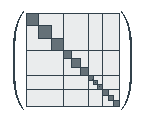
\includegraphics[height = 0.8\linewidth]{../repos/hbp-paper/doc/aistats_talk/logo/hbp_logo_splitting}
  \end{center}
  \vspace{-2ex}
  \captionof{figure}{\textbf{Illustration of sub-blocking.} Here, each diagonal
    block is split into three blocks of equal size.}\label{fig:hbp::subblocking}
}. \Cref{hbp::fig:experiment_fcnn} shows performance curves. In the initial
phase, the BDA can be split into a larger number of sub-blocks without suffering
from a loss in performance. The reduced curvature information is still
sufficient to escape the initial plateau. However, larger blocks have to be
considered in later stages to further reduce the loss efficiently.

The fact that this switch in modularity is necessary is an argument in favor of
the HBP's flexibility to efficiently realize such switches: for this experiment,
the splitting for each block was artificially chosen to illustrate this
flexibility. In principle, the splitting could be decided individually for each
parameter block, and even changed at run time.

\subsubsection{CNN, Matrix-free Exact Curvature Multiplication}

For convolutions, the large number of hidden features prohibits backpropagating
a curvature matrix batch average. Instead, we use exact curvature matrix-vector
products provided within HBP. The CNN possesses sigmoid activations and cannot
be trained by SGD (\Cref{hbp::subfig:experiment_cnn1}). For comparison with
another second-order method, we experiment with a public KFAC
implementation~\citep[see \Cref{hbp::sec:experimentalDetails} for
details]{martens2015optimizing,grosse2016kronecker}.

The matrix-free second-order methods progress fast in the initial stage of the
optimization. However, progress in later phases stagnates. This may be caused by
the limited sophistication of the update rule~\eqref{hbp::equ:linearSystemCG}: if a
small value for $\alpha$ is chosen, the optimizer will perform well in the
beginning (GGN, $\alpha_1$). As the gradients become smaller, and hence more
noisy, the step size limitation is too optimistic, which leads to a slow-down in
optimization progress. A more conservative step size limitation improves the
overall performance at the cost of fewer initial progress (GGN, $\alpha_2$). In
the training phase where damping is ``effective'', our illustrative methods, and
KFAC, exhibit better progress per iteration on the objective than the
first-order competitor Adam, underlining the usefulness of curvature even if
only computed block-wise.

For an impression on performance in terms of run time,
\Cref{hbp::subfig:experiment_cnn2} compares the wall-clock time of one
matrix-free method and the baselines. The HBP-based optimizer can compete with
existing methods and offers potential for further improvements, like
sub-blocking and parallelized CG. Despite the more adaptive nature of
second-order methods, their full power seems to still require adaptive damping,
to account for the quality of the local quadratic approximation and restrict the
update if necessary. The importance of these techniques to properly adapt the
Newton direction has been emphasized in previous works
\citep{martens2010deep,martens2015optimizing, botev2017practical} that aim to
develop fully fletched second-order optimizers. Such adaptation, however, is
beyond the scope of this text.

%%% Local Variables:
%%% mode: latex
%%% TeX-master: "../thesis"
%%% End:
